\documentclass[12pt,fleqn]{report}
\usepackage[utf8]{inputenc}
\usepackage{graphicx}
\graphicspath{{figures/}}
\usepackage[left=30mm, right=30mm, top=30mm, bottom=30mm, includefoot, headheight=16pt]{geometry}
\usepackage{fancyhdr}
\pagestyle{fancy}
\usepackage{natbib}
\usepackage{color}
\usepackage{siunitx}
\usepackage{physics}
\usepackage{dsfont}
\usepackage{csquotes}
\usepackage[colorlinks = true,
            linkcolor = blue,
            urlcolor  = blue,
            citecolor = blue,
            anchorcolor = blue]{hyperref}
\usepackage{mathtools}
\usepackage{wrapfig}
\usepackage{setspace}
\usepackage[font=footnotesize]{caption}
\usepackage[toc,page]{appendix}

\setcounter{chapter}{-1}

\newcommand{\changeurlcolor}[1]{\hypersetup{urlcolor=#1}}
\numberwithin{equation}{section}

\allowdisplaybreaks

\pagestyle{fancy}
\fancyhead{}
% \fancyhead[L]{\rightmark}
\fancyhead[L]{\leftmark}

\let\vec\boldsymbol

\begin{document}

\onehalfspacing

\begin{titlepage}
    \begin{center}
        
        \Huge
        \textbf{Oscillations in magnetic and kinetic energy in the solar atmosphere}
        
        \vspace{0.5cm}
        \LARGE
        A mathematical investigation of the role of resonant absorption and phase mixing in coronal heating and seismology
        
        \vspace{1cm}
        
        \textbf{A. P. K. Prokopyszyn}
        
        \vspace{1cm}
        
        A thesis submitted for the degree of PhD at the University of St Andrews
        
        \vspace{3cm}
        
        
\includegraphics[width=0.3\textwidth]{introduction/st-andrews-shield.png}
        
        \vspace{0.1cm}
        
        \today
        
    \end{center}
\end{titlepage}

% \begin{titlepage}
%   \begin{center}
%       \vspace*{1cm}

%       \textbf{Thesis Title}

%       \vspace{0.5cm}
%         Thesis Subtitle
            
%       \vspace{1.5cm}

%       \textbf{Author Name}

%       \vfill
            
%       A thesis presented for the degree of\\
%       Doctor of Philosophy
            
%       \vspace{0.8cm}
     
%       \includegraphics[width=0.4\textwidth]{university}
            
%       Department Name\\
%       University Name\\
%       Country\\
%       Date
            
%   \end{center}
% \end{titlepage}

\thispagestyle{plain}
\begin{center}
    % \Large
    % \textbf{Linear magneto-kinetic waves in the solar atmosphere}
    
    % \vspace{0.4cm}
    % \large
    % Investigating the role of resonant absorption and phase mixing in coronal heating and seismology
    
    % \vspace{0.4cm}
    % \textbf{Alexander Prokopyszyn}
    
    % \vspace{0.9cm}
    \textbf{Abstract}
\end{center}

\begin{spacing}{1.1}

\noindent 
% This thesis uses mathematical models to help us understand the properties of these waves.

\textbf{Background:} 
% The Sun is a massive and highly dynamic ball of ionised gas (plasma) with a magnetic field extending throughout the solar system. The plasma is frozen to the magnetic field and so magneto-kinetic waves, i.e. propagating oscillations in kinetic and magnetic energy are ubiquitous in the solar atmosphere. 
% This thesis uses the fundamental equations of magnetohydrodynamics (the MHD equations) to build our understanding of wave behaviour in the solar corona. The MHD equations bring together equations from hydrodynamics (the study of non-ionised fluids) with Maxwell's electromagnetic equations. This means that the dynamics of plasma shares a lot of properties with the dynamics of non-ionised fluids, however, some phenomena occurs exclusively in plasma and cannot occur in a regular non-ionised fluid. 
The sun is a massive and highly dynamic ball of plasma, and magneto-kinetic waves (oscillations in kinetic and magnetic energy) are commonplace throughout its atmosphere. Since the plasma conducts electricity, we model the fluid using magnetohydrodynamics (MHD) instead of hydrodynamics which is usually used for non-ionised fluids. We study two MHD wave phenomena called phase mixing and resonant absorption. These are both phenomena which occur exclusively in MHD fluids and cannot occur in hydrodynamic fluids. We study their implications for the coronal heating problem and coronal seismology. The solar surface is significantly denser than the atmosphere and we model it as solid wall. In other words, we impose line-tied boundary conditions at the solar surface where the velocity is set equal to zero.
% The coronal heating problem relates to the question; `why is the corona approximately $10^6\si{.K}$ while the photosphere which is closer to the centre of the Sun is only about $10^4\si{.K}$?' Coronal seismology is a technique where mathematical models are used to infer hard to measure quantities, e.g. the coronal magnetic field strength or density gradients from easier to measure quantities e.g. wave frequencies and damping time.

\textbf{Aims:}
% \textcolor{red}{The second chapter aims to study the simplest know MHD wave, namely Alfv\'en waves. The goal is to explain some of the key ideas which will be developed throughout this thesis.} After the introduction, the second chapter studies the simplest known MHD wave, namely, Alfv\'en waves. We study the resonances which can form in coronal loops and the effects introduced by allowing waves to leak out of the corona and by switching from a sinusoidal driver to a broadband driver.
1) Chapter \ref{chap:ideal_footpoint_driven_alfven_waves} aims to introduce some of the key properties of footpoint driven Alfv\'en waves (a type of MHD wave) which are relevant for the rest of this thesis.
2) Chapter \ref{chap:resistive_phase_mixed_alfven_waves} aims to calculate an upper bound for the heat that can be produced by linear phase-mixed Alfv\'en at observed frequencies and amplitudes to assess its viability as a coronal heating mechanism.
3) Chapter \ref{chap:resonant_absorption_in_an_oblique_field} aims to test if line-tied boundary conditions still apply in a resonant absorption experiment where the transverse length-scales can be very short.
% \textcolor{red}{The fourth chapter aims to test if the boundary layers formed in resonant absorption experiments where the background field is oblique to the transition region are physical or a result of imposing line-tied boundary conditions.} The fourth chapter studies resonant absorption for the case where the background magnetic field is tilted to be oblique to the transition region. Imposing line-tied boundary conditions at the transition region generates large-amplitude boundary layers. We test if these boundary layers are physical and not a fictitious result arising from the use of line-tied boundary conditions.

\textbf{Methods:} We take an analytic and theoretical approach when solving each of these problems. Then check the results numerically.

\textbf{Results:} 1) We show that the growth of energy in closed loops for a sinusoidal footpoint driver is highly dependent on the driver frequency. If a resonance is excited, then the energy grows quadratically with time, and for a broadband driver, the energy grows linearly on average. If the loop is partially-closed (i.e. only a fraction of the wave amplitude reflects at the boundary), the energy will converge towards a steady-state where the loop's energy remains constant with time. 
2) We calculate an upper bound for the heat that can be produced by phase-mixed Alfv\'en waves and find that it is on average too small to play a significant role in coronal heating. 
3) We show that imposing line-tied boundary conditions can cause the model generate unphysically large boundary layers when the transverse length-scales are very short. However, researchers may wish to continue to use them in their models for their simplicity and ability to significantly reduce computation time if they understand and are aware of their flaws.
% However, the energy of the boundary layers does not grow with time and so we argue its okay to use line-tied boundary conditions in future models provided it is understood that the boundary layers produced are mostly unphysical.

\end{spacing}

% \chapter*{Dedication}
% To mum and dad
 
% \chapter*{Declaration}
% I declare that..
 
% \chapter*{Acknowledgements}
% I want to thank...
 
\tableofcontents

\chapter{Introduction}
\label{chap:introduction}
% Magnetohydrodynamic (MHD) waves are commonplace in the solar atmosphere and have been observed over the last two decades as a consequence of new, improved imaging and spectroscopic instruments (see, e.g. \citealt{Tomczyk2007,McIntosh2011,McIntosh2012,DeMoortel2012}).
% The primary aim is to study the properties of these waves. This section aims to introduce some of the key results in the literature which are relevant to the rest of the thesis. In Section \ref{sec:solar_atmosphere} we give a brief introduction to the solar atmosphere. In Section \ref{sec:mhd equations} we introduce the MHD equations which form the basis of all the mathematical models used throughout this thesis.

% One of the cool things about solar physics is that despite the sun being 100s of thousands of kilometres away by using maths, physics and observational data we are able to develop a surprisingly good understanding of how it works.

The Sun is the brightest and most energetic object in the solar system. Despite it being $1.5\times10^8\si{.km}$ away, our understanding of how it works has dramatically improved over the last century. Solar physics has played a vital role in some of the most important discoveries of the last century. For example, before the 20th century, the fuel source for the Sun was a complete mystery. It was not until the early 20th century that Hydrogen's fusion into Helium was first proposed as the dominant process that powers the stars. More recently, the solar neutrino problem was solved due to developments in particle and quantum physics. The solar neutrino problem concerned a large discrepancy between solar neutrinos' flux as predicted from the Sun's luminosity and measured directly. The difference was first observed in the mid-1960s and finally resolved around 2002. Another fundamental discovery was the derivation of the MHD equations (see Section \ref{sec:mhd equations}) which combines the equation of fluid dynamics with electromagnetism. These equations enable the plasma, which makes up the Sun to be modelled and played a key role in allowing Eugene Parker to predict the solar wind's existence in 1957. The MHD equations are also currently being used to develop space weather prediction models to give early warnings of dangerous flares and coronal mass ejections, see for example, \citet{Feynman2000}.

Over recent decades, due to improvements in our observational instruments, we are now able to measure wave amplitudes and frequencies in the solar atmosphere directly. This thesis focuses on studying linear magneto-kinetic waves in the solar atmosphere. Improving our understanding of these waves could lead to coronal seismology developments. It may help solve one of the biggest problems in solar physics, namely, the coronal heating problem (see Section \ref{sec:coronal_heating_problem}). Coronal seismology is a technique where mathematical models are used to infer hard to measure quantities, e.g. the coronal magnetic field strength or density gradients from easier to measure quantities, e.g. wave frequencies and damping time. We take a theoretical, as opposed to an observational approach to build our simple models. We calculate analytic solutions which we verify numerically. Most of the code used for this thesis, including LaTeX files, is available on GitHub via the following URL:
\[\text{\href{https://github.com/aleksyprok/apkp_thesis}{https://github.com/aleksyprok/apkp\_thesis}}\]
In this chapter, we introduce some of the solar atmosphere's critical properties relevant to this thesis. After that, we will introduce the MHD equations which allow us to model plasma dynamics we will be studying. In Section \ref{sec:mhd_waves_dispersion_relation}, we model waves in a domain where the background quantities are uniform and introduce some of the key aspects and terminology used in solar MHD wave theory. Finally, in Section \ref{sec:mhd_waves_power_spectrum}, we discuss recent observations of waves in the solar atmosphere and show how the energy distributes as a function of wave frequency.

\section{Solar atmosphere}
\label{sec:solar_atmosphere}

The solar atmosphere refers to the outer layer of gas and plasma surrounding the Sun. It is defined as the part of the Sun from which photons can escape directly into space. We split the atmosphere into four regions: the photosphere, chromosphere, transition region and corona. The regions form approximate concentric spherical shells around the Sun. However, this picture breaks down at, for example, prominences/filaments, which are cool and dense loop structures which can extend high into the corona. With that in mind, when viewing the Sun at a global scale, it is useful to model it in terms of four distinct, but highly coupled layers.

\begin{figure}[!htp]
    \centering
    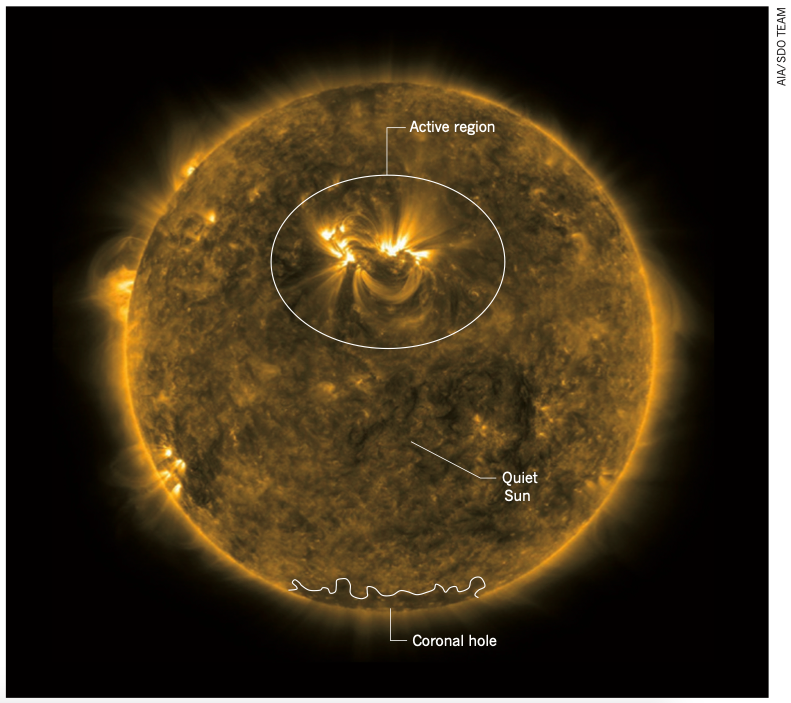
\includegraphics[width=\textwidth]{introduction/active_region_coronal_hole_quiet_sun.png}
    \caption{At a temperature of about 1 million kelvin, this image of coronal plasma was taken from the Atmospheric Imaging Assembly (AIA) instrument on the Solar Dynamics Observatory (SDO). We took the labels from \citet{Cargill2011}. It also offers an example of solar physicists labelling different solar atmosphere parts as either an active region, coronal hole or quiet sun.}
    \label{fig:active_region_quiet_sun_coronal_hole}
\end{figure}

\begin{figure}[!htp]
    \centering
    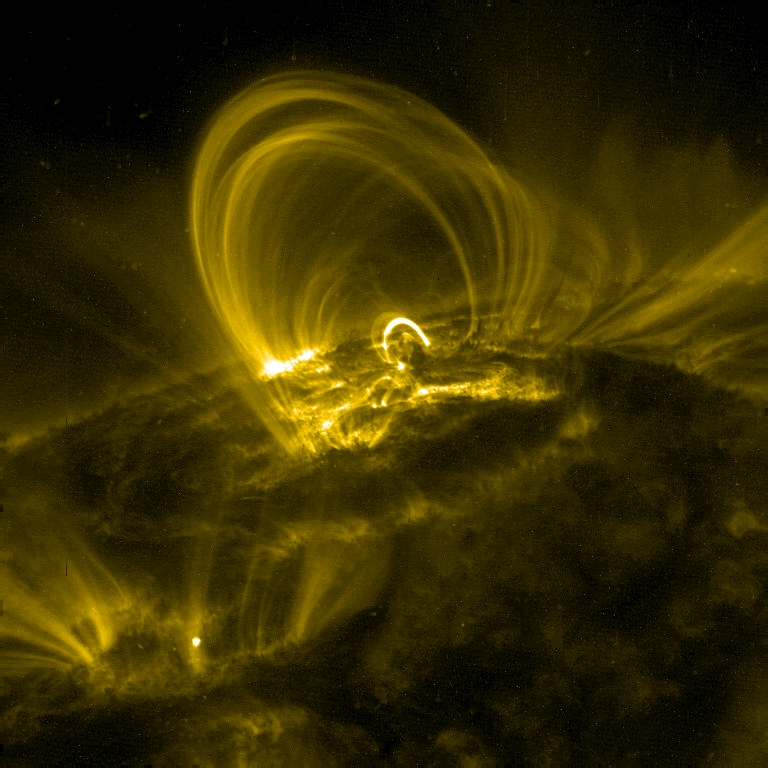
\includegraphics[width=\textwidth]{figures/introduction/coronal_loop_trace.jpg}
    \caption{This image of coronal loops was taken using the TRACE (Transition Region and Coronal Explorer) instrument (courtesy \citet{images_of_coronal_loops}). It shows coronal plasma at a temperature of about 1 million kelvin.}
    \label{fig:coronal_loops_trace}
\end{figure}


\begin{figure}[!htp]
    \centering
    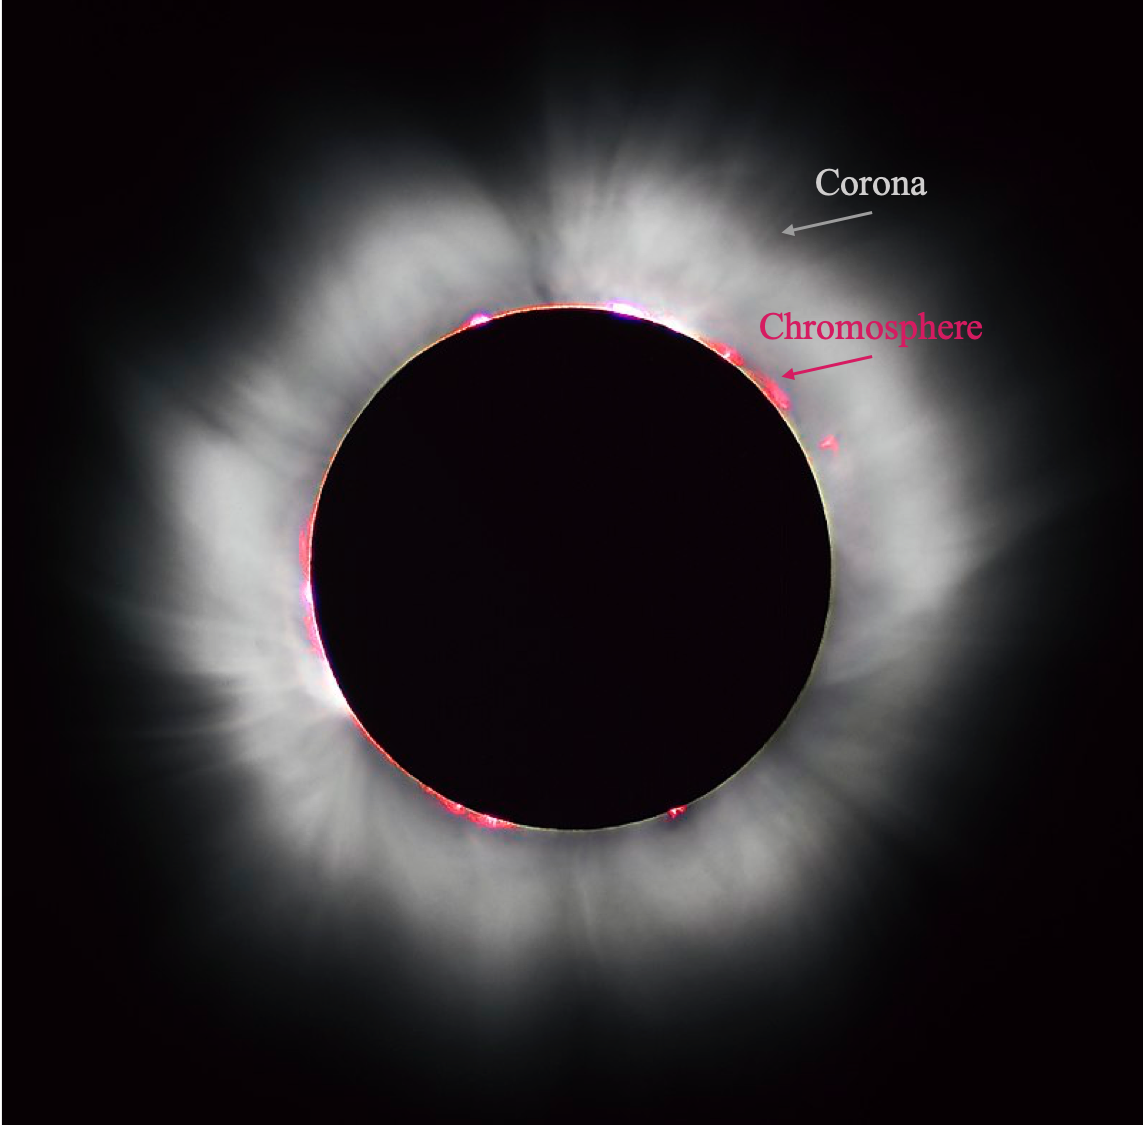
\includegraphics[width=\textwidth]{introduction/eclipse_1999.png}
    \caption{This photo taken in France during the 1999 total eclipse (courtesy Wikimedia, User: Luc Viatour). The chromosphere is emitting a pink/red light close to the disc. The faint white glow around the disk shows white light from the photosphere being Thompson scattered by the corona.}
    \label{fig:total_eclipse1999}
\end{figure}

\begin{figure}[!htp]
    \centering
    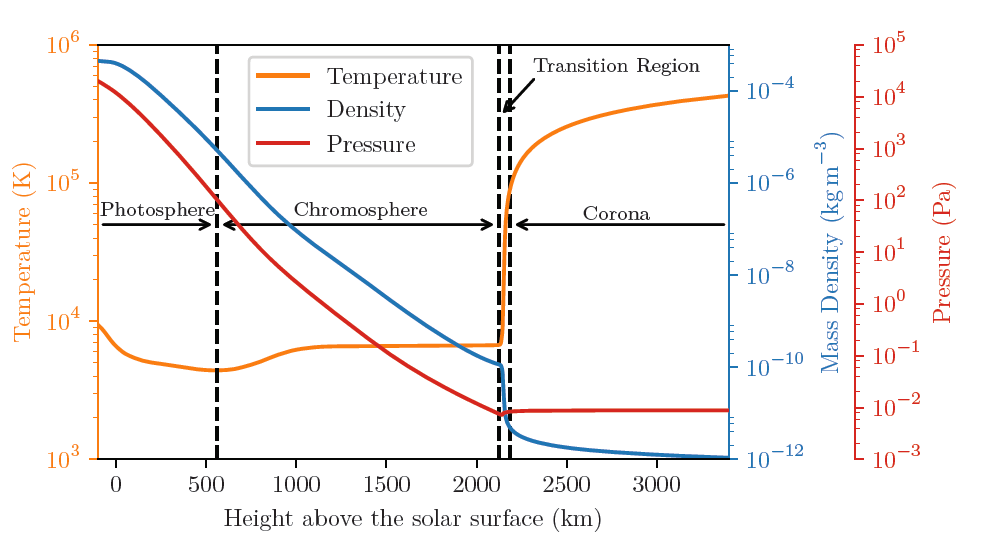
\includegraphics[width=\textwidth]{introduction/VAL.png}
    \caption{The VAL model \citep{Vernazza1981} of the solar atmosphere (courtesy \citet{Williams2018}).}
    \label{fig:VAL_atmosphere}
\end{figure}

\begin{table}[!htp]
    \centering
    \begin{tabular}{c c c c}
        \hline
         & Coronal hole & Quiet Sun & Active region \\
        \hline
        \underline{Corona}  \\
        Conduction & 60 & 200 & $10^3\text{-}10^4$ \\
        Radiation & 10 & 100 & 5000 \\
        Solar wind & 700 & $<50$ & $<100$ \\
        \hline
        Total & 800 & 300 & 10,000 \\
        \hline
        \underline{Chromosphere} \\
        Radiation & 4000 & 4000 & 20,000
        
    \end{tabular}
    \captionof{table}{Order-of-magnitude energy-loss fluxes in $\si{W.m^{-2}}$ \citep{Withbroe1977, Priest2014}.}
    \label{tab:energy_losses_corona_chromosphere}
\end{table}

We label different parts of the solar atmosphere as either an active region, coronal hole or quiet sun (see Figure \ref{fig:active_region_quiet_sun_coronal_hole}). An active region is an area with a strong magnetic field. It is common for sunspots to form in active regions. These are usually the locations where the largest flares and coronal mass ejections occur. Coronal holes are the polar regions of the Sun, which look dark in the X-ray emission. In coronal holes, the magnetic field is usually unipolar and opens towards the interplanetary space. Finally, the quiet Sun usually refers to Sun regions that do not lie in either active regions or coronal holes. Note that active regions and the quiet Sun often contain closed loops, like those shown in Figure \ref{fig:coronal_loops_trace}. We refer to these loops as closed because their magnetic field does not extend beyond the solar atmosphere. In contrast, the coronal holes' field lines are referred to as open because they extend far out into the solar system before eventually looping back or connecting with the interplanetary medium.

Figure \ref{fig:VAL_atmosphere} shows data from what is commonly referred to as the Vernazza Avrett and Loeser (VAL) \citep{Vernazza1981} model of the solar atmosphere. It is useful for approximating average values of physical quantities. However, the solar atmosphere is, in reality, a highly inhomogeneous, time-dependent plasma. Figure \ref{fig:VAL_atmosphere} shows that the lowest region is the photosphere. It is the region where most photons, at visible light frequencies, escape into outer space. The chromosphere lies above the photosphere and emits significantly less light than the photosphere. It is only visible with the naked eye during total solar eclipses (see red / pink light in Figure \ref{fig:total_eclipse1999}). The transition region lies between the chromosphere and the corona. Across the transition region, the temperature changes rapidly from approximately $10^5\si{.K}$ to $10^6\si{.K}$. Finally, the corona lies above the chromosphere and transition region. As with the chromosphere, it emits significantly less light than the photosphere and is only visible with the naked eye during total solar eclipses as a white glow (see Figure \ref{fig:total_eclipse1999}). Note that the corona Thompson scatters white light from the photosphere. The intrinsic colour of the corona is not white. However, the chromosphere's inherent colour is indeed the pink/red colour seen in Figure \ref{fig:total_eclipse1999}.

\section{Coronal heating problem}
\label{sec:coronal_heating_problem}

The chromospheric and coronal heating problem relates to the question; 'why are they so hot?' It remains one of the biggest unsolved problems in solar physics. Figure \ref{fig:VAL_atmosphere} shows that the temperature increases with distance from the photosphere in the corona and chromosphere. Looking at Figure \ref{fig:VAL_atmosphere}, two questions come to mind. Why does the temperature increase with distance away from the Sun's core? Intuitively, the temperature should decrease away from a heat source. Since the temperature is higher in the corona and chromosphere, this means that conduction is an energy loss mechanism. They are also optically thin, which means they lose more energy via radiation than they gain. So what is balancing the conductive and radiative losses in the chromosphere and corona?
The energy losses are balanced by converting kinetic and magnetic energy into heat via Ohmic and viscous dissipation \citep{Klimchuk2015}. However, we do not have a verified model giving a precise description of how the temperatures are maintained.

Regarding the first question, we now understand why the solar atmosphere's temperature increases with distance from the Sun's core. For example, \citet{Martens2010} successfully models a similar temperature profile  (although a detailed description of the heating source is still unknown). These models use the internal energy equation with a user-defined heating function superimposed. This heating function simulates the Ohmic and viscous dissipation of magnetic and kinetic energy. They find that even if the heating function is more significant at the footpoints, their models still produce the same basic structure as the solar atmosphere. This counter-intuitive temperature profile is partly explained by the fact that for coronal/chromospheric plasma, the radiative losses can decrease with rising temperature (see for example \citealt{Klimchuck2008}).
However, a detailed description of the primary mechanism(s) by which magnetic and kinetic energy dissipates in the corona has yet to be provided.

In the closed corona, the proposed heating mechanisms can be split into two categories: reconnection and wave heating mechanisms. In for example \citet{vanBallegooijen2011}, \citet{Howson2020} they model both mechanisms and compare them against each other. Reconnection mechanisms rely on the slow stressing of the magnetic field. We define slow motions as having a period longer than the Alfv\'en travel time of a coronal loop. In Section \ref{sec:case_where_omega=omega_n} we show that if the driving footpoint motions are longer than the Alfv\'en travel time of the loop then this causes the loop to stretch resulting in a large build-up in magnetic energy compared with a small growth in kinetic energy. We show that if the driving motions period is shorter than the Alfv\'en travel time of the loop then the growth in kinetic and magnetic energy is approximately equal. Therefore, for reconnection models, the primary dissipation mechanism is resistive since the amount of free magnetic energy is usually much greater than the amount of free kinetic energy. The amount of free magnetic and kinetic energy associated with the wave is assumed to be approximately equal. Therefore, for wave heating mechanisms the primary dissipation mechanism is usually viscous because the viscous Reynolds number (see Equation \ref{eq:visc_reynolds_number}) is much smaller than the magnetic Reynolds number (see Equation \ref{eq:mag_reynolds_number}).

This thesis will investigate the dissipation of phase mixed Alfv\'en waves and their role in coronal heating. The dissipation of Alfvén waves has been the basis of many coronal heating models (see review by \citealt{Arregui2015} and references therein). Phase mixing was first suggested as a coronal heating mechanism by \citet{Heyvaerts1983}. Phase mixing is the process where gradients perpendicular to the field build-up due to Alfvén waves propagating on field lines with a spatial gradient in Alfvén travel time. This process leads to neighbouring waves moving out of phase with each other; hence the name phase mixing. Other notable mechanisms are: resonant absorption \citep{Ionson1982}, reflection-driven Alfvén wave turbulence \citep{Hollweg1986a,vanBallegooijen2011,Shoda2019}, turbulence triggered via the tearing mode or Kelvin-Helmholtz instability \citep{Browning1984,Antolin2016,Antolin2018} and coupling with compressive modes \citep{Kudoh1999, Antolin2010}.

Table \ref{tab:energy_losses_corona_chromosphere} shows order-of-magnitude estimates for the power-losses (per unit area) in the corona and chromosphere. Note that the mean radiation from the photosphere is significantly greater at about $0.63\times 10^8\si{.W.m^{-2}}$. It is sometimes useful to consider the energy losses per unit volume rather than by per area. The chromosphere’s per unit volume radiative losses can be calculated from the total radiative losses divided by the volume. 
Taking the height difference between the top and bottom of the chromosphere as $1500\si{.km}$ gives the average radiative losses in an active region chromosphere per unit volume as $1.33\times10^{-2}\si{.W.m^{-3}}$. To help get an intuitive idea of how much heat this is, this means that a $1\si{.W}$ light-emitting diode emits about the same radiation as an Olympic sized swimming pool of chromosphere. It is worth noting that the chromosphere and corona are very sparse compared with the photosphere and so a relatively small amount of heat can lead to a large temperature change.
% Taking the height difference between the top and bottom of the chromosphere as $1500\si{.km}$ gives the average radiative losses in the Quiet sun chromosphere per unit volume as $\approx 3\times10^{-3}\si{.W.m^{-3}}$. To put this number in perspective, the average radiative losses from a human is about $100\si{.W}$\footnote{Radiative losses of a human was calculated by using the Stefan-Boltzmann law, where the area of a human was taken to be 2\si{.m^2}, the emissivity of human skin to be unity \citep{emissivity_of_materials}, the temperature of a human as 306\si{.K} and room temperature as 293\si{.K}.}. Therefore, taking the volume of a human as $0.1\si{.m^3}$ gives the radiative losses per volume as $10^3\si{.W.m^{-3}}$. This means that per volume humans emit of the order a million times as much radiation!
% This shows that although the chromosphere and corona have large temperatures they are very sparse and so per volume their radiation is relatively small. 
Note that Table \ref{tab:energy_losses_corona_chromosphere} shows the radiative losses are greater in the chromosphere than in the corona. This is interesting as chromospheric and coronal heating problem is usually referred to as simply the coronal heating problem despite the chromospheric radiative losses being greater.

\section{MHD equations}
\label{sec:mhd equations}

A large fraction of the solar atmosphere is ionised \citep{Shimizu2018} due to the high temperature. The high temperature allows the orbital electrons to break their bonds with their corresponding ions and form free electrons. Therefore, the gas can conduct electricity and is hence a plasma. To study the plasma, we use Magnetohydrodynamics (MHD). The MHD equations are formed by combining equations from electromagnetism with equations from fluid dynamics. Different forms of the MHD equations are used in different contexts. In sections \ref{sec:faradays_law}-\ref{sec:intro_total_energy_eqn} we discuss each of the MHD equations in SI base units.

% \begin{figure}
%     \centering
%     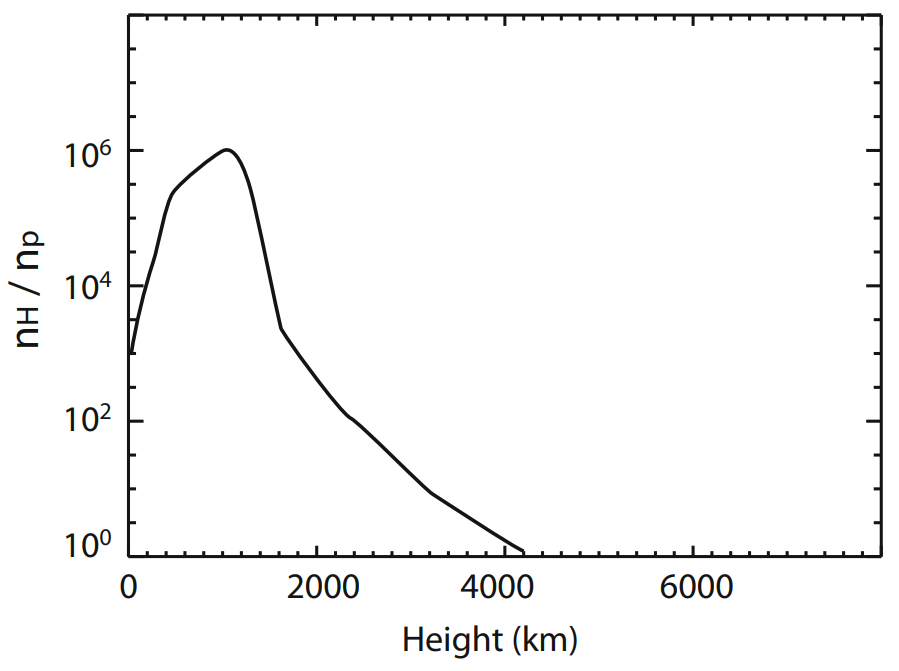
\includegraphics[width=0.5\textwidth]{figures/introduction/partial_ionisation.png}
%     \caption{This figure was taken from \citet{Shimizu2018}. It shows the partial ionisation fraction, $n_H/n_p$, as a function of height in the solar atmosphere, where $n_H$ and $n_p$ denotes the number density of the neutral hydrogen atoms and protons respectively.}
%     \label{fig:partial_ionisation}
% \end{figure}

\subsection{Assumptions}
\label{sec:intro_assumptions}

This thesis is primarily concerned with studying waves in the corona which is assumed to be fully ionised. The Sun's atmosphere is approximately 74\% Hydrogen 25\% Helium and 1\% other elements \citep{sun_vital_statistics}. At typical coronal temperatures, say $10^6\si{.K}$, an electron's thermal energy is approximately $86\si{.eV}$. This is greater than the ionisation energies of Hydrogen and Helium which have first ionisation energies of approximately $14\si{.eV}$ and $25\si{.eV}$ and Helium's second ionisation energy is approximately $54\si{.eV}$ \citep{Lide2003}. Also, the ionisation fraction as a function of height has been estimated in, for example, \citet{Shimizu2018} and suggests that the plasma in the corona is nearly completely ionised. Therefore, in this thesis, we will often model the plasma as fully ionised Hydrogen plasma.

We model the plasma as collisional and assume that collisional transport theory is valid. In \citet{Richardson2019}, they list six conditions for collisional transport theory to be valid. In the strong magnetic field limit, where $\omega_{ce}/\nu_e \gg 1$ (see Table \ref{tab:fundamental_plasma_paramter}) we require
\begin{gather}
    \label{eq:length_scale_condition_parallel}
    L_{||} \gg \lambda_{Te}, \lambda_{Ti}, \\
    \label{eq:length_scale_condition_perpendicular}
    L_\perp \gg \sqrt{\lambda_{Te} r_e}, \sqrt{\lambda_{Ti} r_e}
\end{gather}
where $L_{||}$, $L_\perp$ denote the macroscopic length scales parallel and perpendicular to the magnetic field respectively. In the absence of a magnetic field, we require
\begin{equation}
    \label{eq:length_scale_condition}
    L \gg \lambda_{Te}, \lambda_{Ti},
\end{equation}
where $L$ denotes the macroscopic length scales. For fully ionised Hydrogen plasma, typical values in the corona are,
\begin{gather}
    \begin{aligned}
    \frac{\omega_{ce}}{\nu_e} &= \frac{1}{3.64\times10^{-6}}\frac{eBT^{3/2}}{m_en_e\ln\Lambda} \\
    &\approx 2.42\times10^5\qty(\frac{20}{\ln\Lambda})\qty(\frac{B}{10^{-3}\si{.T}})\qty(\frac{T_e}{10^6\si{.K}})^{3/2}\qty(\frac{10^{15}\si{.m^{-3}}}{n_e}),
    \end{aligned} \\
    \begin{aligned}
    \lambda_{Te} &= \frac{1}{3.64\times10^{-6}}\frac{\sqrt{k_B/m_e}}{\ln\Lambda}\frac{T_e^2}{n_e} \\
    &\approx 0.53\times10^5\qty(\frac{20}{\ln\Lambda})\qty(\frac{T_e}{10^6\si{.K}})^2\qty(\frac{10^{15}\si{.m^{-3}}}{n_e})\si{.m}, 
    \end{aligned} \\
    \begin{aligned}
    \lambda_{Ti} &= \frac{1}{6.00\times10^{-6}}\frac{\sqrt{k_B/m_p}}{\ln\Lambda}\frac{T_i^2}{n_i} \\
    &\approx 0.76\times10^5\qty(\frac{20}{\ln\Lambda})\qty(\frac{T_i}{10^6\si{.K}})^2\qty(\frac{10^{15}\si{.m^{-3}}}{n_i})\si{.m}, 
    \end{aligned} \\
    \begin{aligned}
    r_e & \approx \frac{\sqrt{m_e k_B T_e}}{eB} \\
    &\approx 2.21 \times 10^{-2}\qty(\frac{T_e}{10^6\si{.K}})\qty(\frac{10^{-3}\si{.T}}{B})\si{.m}.
    \end{aligned}
\end{gather}
Therefore, provided the macroscopic length scales are greater than about $1\si{.Mm}$ Equations \eqref{eq:length_scale_condition_parallel}-\eqref{eq:length_scale_condition} should be approximately satisfied.

\begin{table}
    \centering
    {\renewcommand{\arraystretch}{2}% for the vertical padding
        \begin{tabular}{|c|c|c|c|c|}
            \hline
             Name & Symbol & Gaussian units & SI units \\
             \hline
              {\renewcommand{\arraystretch}{0.8}\begin{tabular}[x]{@{}c@{}}Electron\\gyrofrequency\end{tabular}} & $\omega_{ce}$ & $\dfrac{eB}{m_e c}$ & $\dfrac{eB}{m_e}$  \\
             {\renewcommand{\arraystretch}{0.8}\begin{tabular}[x]{@{}c@{}}Ion\\gyrofrequency\end{tabular}} & $\omega_{ci}$ & $\dfrac{ZeB}{m_i c}$ & $\dfrac{ZeB}{m_i}$ \\
             {\renewcommand{\arraystretch}{0.8}\begin{tabular}[x]{@{}c@{}}Electron\\collision rate\end{tabular}} & $\nu_e$ & $2.91\times10^{-6}\dfrac{n_e \ln\Lambda}{T_e^{3/2}}\si{.s^{-1}}$ & $3.64\times10^{-6}\dfrac{n_e \ln\Lambda}{T_e^{3/2}}\si{.s^{-1}}$ \\
             {\renewcommand{\arraystretch}{0.8}\begin{tabular}[x]{@{}c@{}}Ion\\collision rate\end{tabular}} & $\nu_i$ & $4.80\times10^{-8}\dfrac{Z^4n_i \ln\Lambda}{\sqrt{T_i^3m_i/m_p}}\si{.s^{-1}}$ & $6.00\times10^{-8}\dfrac{Z^4n_i \ln\Lambda}{\sqrt{T_i^3m_i/m_p}}\si{.s^{-1}}$ \\
             {\renewcommand{\arraystretch}{0.8}\begin{tabular}[x]{@{}c@{}}Electron\\thermal speed\end{tabular}} & $v_{Te}$ & $\sqrt{\dfrac{k_BT_e}{m_e}}$ & $\sqrt{\dfrac{k_BT_e}{m_e}}$ \\
             {\renewcommand{\arraystretch}{0.8}\begin{tabular}[x]{@{}c@{}}Ion\\thermal speed\end{tabular}} & $v_{Ti}$ & $\sqrt{\dfrac{k_BT_i}{m_i}}$ & $\sqrt{\dfrac{k_BT_i}{m_i}}$ \\
             {\renewcommand{\arraystretch}{0.8}\begin{tabular}[x]{@{}c@{}}Electron\\gyroradius\end{tabular}} & $r_e$ & $\dfrac{v_{Te}}{\omega_{ce}}$ & $\dfrac{v_{Te}}{\omega_{ce}}$ \\
             {\renewcommand{\arraystretch}{0.8}\begin{tabular}[x]{@{}c@{}}Ion\\gyroradius\end{tabular}} & $r_i$ & $\dfrac{v_{Ti}}{\omega_{ci}}$ & $\dfrac{v_{Ti}}{\omega_{ce}}$ \\
             {\renewcommand{\arraystretch}{0.8}\begin{tabular}[x]{@{}c@{}}Electron\\mean free path\end{tabular}} & $\lambda_{Te}$ & $\dfrac{v_{Te}}{\nu_e}$ & $\dfrac{v_{Te}}{\nu_e}$ \\
             {\renewcommand{\arraystretch}{0.8}\begin{tabular}[x]{@{}c@{}}Ion\\mean free path\end{tabular}} & $\lambda_{Ti}$ & $\dfrac{v_{Ti}}{\nu_i}$ & $\dfrac{v_{Ti}}{\nu_i}$ \\
             \hline
        \end{tabular}
    }
    \captionof{table}{This table lists some of the fundamental plasma parameters. The Gaussian formulas were taken from \citet{Richardson2019} which we then converted into SI base units. The collision rates are for completely ionised plasmas. $B$ denotes the magnetic field strength, $e$ denotes the elementary charge, $c$ denotes the speed of light, $m_e$, $m_p$ denote the mass of an electron and proton respectively, $Z$ gives the charge state, i.e. the number of protons in an ion, $n_e$, $n_i$ denote the electron and ion number densities respectively, $\ln \Lambda$ denotes the Coulomb logarithm, $T_e$, $T_i$ denotes the temperature of the electrons and ions respectively and $k_B$ denotes the Boltzmann constant.}
    \label{tab:fundamental_plasma_paramter}
\end{table}

\subsection{Faraday's law}
\label{sec:faradays_law}

Faraday's law is given by
\begin{equation}
    \label{eq:faradays_law}
    \curl\vec{E}=-\pdv{\vec{B}}{t}.
\end{equation}
$\vec{B}$ is the magnetic induction. In solar or astrophysical contexts, it is referred to as the magnetic field strength. In this thesis, $\vec{B}$ will hereafter be referred to as the magnetic field strength. $\vec{E}$ denotes the electric field. Finally, time is denoted with $t$.

\subsection{Amp\`ere's law}
\label{sec:amperes_law}

Amp\`ere's's law is given by
\begin{equation}
    \label{eq:amperes_law}
    \curl{\vec{B}}=\mu_0\vec{j}+\underbrace{\frac{1}{c^2}\pdv{\vec{E}}{t}}_{\approx\,0}
\end{equation}
We approximate the magnetic permeability, $\mu_0$, by its value in a vacuum, namely,
\[\mu_0=4\pi\times10^{-7}\si{.henry.m^{-1}}.\]
The current density is denoted with $\vec{j}$. We approximate the speed of light, $c$, with its value in a vacuum, namely,
\[c=\sqrt{\mu_0\epsilon_0}\approx3.00\times10^8\si{.m.s^{-1}},\]
where $\epsilon_0$ is the permittivity of free space in a vacuum. 

In this thesis, we neglect last term in Equation \eqref{eq:amperes_law}, called the displacement current. Replacing the time derivative with $1/t_0$, and $\vec{E}$ with $E_0$ means that
\[\abs{\frac{1}{c^2}\pdv{\vec{E}}{t}}\approx\frac{1}{c^2}\frac{E_0}{t_0},\]
where $E_0$ and $t_0$ denotes the typical size of their respective quantities. From Faraday's law, Equation \eqref{eq:faradays_law}, it follows that
\[\frac{E_0}{l_0}\approx \frac{B_0}{t_0},\]
where $B_0$ and $l_0$ denote the typical size of their respective quantities. Letting
\[v_0=\frac{l_0}{t_0},\quad \frac{B_0}{l_0}\rightarrow|\curl\vec{B}|,\]
it follows that
\[\abs{\frac{1}{c^2}\pdv{\vec{E}}{t}}\approx\frac{v_0^2}{c^2}\abs{\curl{\vec{B}}},\]
where $v_0$ here denotes a typical speed. Hence, we can neglect the displacement current, provided
\begin{equation}
    \label{eq:v0_less_c}
    v_0\ll c.
\end{equation}
This thesis is interested in waves in the corona. It is very rare for waves to have a velocity amplitude which exceeds the local Alfv\'en speed, $v_A$, given by
\begin{equation}
    v_A\approx\frac{\abs{\vec{B}}}{\sqrt{{\mu}_0\rho}},
\end{equation}
where $\rho$ denotes the plasma density. In the corona, the Alfv\'en speed is approximately $10^6\si{.m.s^{-1}}$ and so condition \eqref{eq:v0_less_c} is satisfied.

% \subsection{Gauss's law}

% Gauss's law is given by
% \begin{equation}
%     \label{eq:gausss_law}
%     \div{\vec{E}}=\underbrace{\frac{\rho^*}{\epsilon_0}}_{\approx\,0},
% \end{equation}
% where $\rho^*$ is the charge density.

\subsection{Solenoidal constraint}

The solenoidal constraint states that
\begin{equation}
    \div{\vec{B}}=0.
\end{equation}
Physically, this equation states that a magnetic field can have no sources or sinks, i.e. no monopoles.

\subsection{Ohm's law}

\citet{Priest2014} shows that for fully ionised plasma, Ohm's law is given by
\begin{equation}
    \label{eq:ohms_law}
    \vec{E}+\vec{v}\cross\vec{B}=\underbrace{\frac{\vec{j}}{\sigma}}_{\text{Direct / Pedersen term}}+\underbrace{\frac{1}{n_ee}\vec{j}\cross\vec{B}}_{\text{Hall term}},
\end{equation}
where the electron inertia and electron pressure gradient terms have been neglected. We denote the plasma velocity with $\vec{v}$. The Cowling conductivity, $\sigma$, is given by
\begin{equation}
    \sigma = \frac{n_ee^2}{m_e\nu_e}.
\end{equation}
Plugging in typical coronal values, the resistivity coefficents can be approximated by
\begin{gather}
    \frac{1}{\sigma}\approx1.37\times10^{-6}\qty(\frac{T}{10^6\si{.K}})^{-3/2}\si{.mho.m^{-1}},  \\
    \frac{\abs{\vec{B}}}{en_e}\approx6.24\,\qty(\frac{\abs{\vec{B}}}{10^{-3}\si{.T}})\qty(\frac{10^{15}\si{.m^{-3}}}{n_e}).
\end{gather}
The coulomb logarithm, $\ln\Lambda$, lies between 5 and 20 and has a weak temperature dependence. For coronal plasma, a suitable approximation is $\ln\Lambda\approx20$. It is tempting to neglect the direct current term in favour of the Hall term. However, the Hall term is dependent only on currents parallel to the field. Throughout this thesis, the currents perpendicular to the field dominate.

\subsection{Mass continuity}

The mass continuity equation is given by
\begin{equation}
    \label{eq:mass_continuity}
    \pdv{\rho}{t}+\div(\rho\vec{v})=0.
\end{equation}
The plasma's mass density is denoted by $\rho$. Physically this equation states that the rate of mass change in a volume is given by the total flux of mass moving in or out of the volume.

\subsection{Momentum equation}
The most general from of the momentum equation / equation of motion which we believe is relevant for this thesis is
\begin{equation}
    \label{eq:momentum}
    \rho\frac{D\vec{v}}{Dt}=\underbrace{\vec{j}\cross\vec{B}}_{\text{Lorentz force}}-\underbrace{\grad p}_{\text{Pressure force}}-\underbrace{\rho g_\odot \vec{\hat{r}}}_{\text{Gravitational force}}+\underbrace{\div\vec{\sigma}_{Brag}}_{\text{Viscous force}}.
\end{equation}
Here the $D/Dt$ operator denotes the material derivative. The plasma pressure is denoted with $p$.

The first term on the right-hand side of Equation \eqref{eq:momentum} is the Lorentz force. The $\rho^*\vec{E}$ term in the more general form of the Lorentz force has been neglected, where $\rho^*$ denotes the charge density. This is because we model the plasma as electrically neutral. \citet{Priest2014} shows that the plasma can be modelled as electrically neutral provided the length scales of the system, $l_0$, are greater than the Debye length, $\lambda_D$. The Debye length is approximated by
\begin{equation}
    \lambda_D\approx2.18\times10^{-3}\qty(\frac{T}{10^6\si{.K}})^{1/2}\qty(\frac{10^{15}\si{.m^{-3}}}{n})^{1/2}\si{.m}.
\end{equation}
The Lorentz force is commonly split into two components,
\begin{equation}
    \vec{j}\cross\vec{B}=\underbrace{\frac{1}{\mu_0}(\vec{B}\vdot\grad)\vec{B}}_{\text{Magnetic tension force}}\underbrace{-\grad\qty(\frac{B^2}{2\mu_0})}_{\text{Magnetic pressure force}},
\end{equation}
where 
\[\frac{B^2}{2\mu_0}=\frac{\vec{B}\vdot\vec{B}}{2\mu_0},\]
is commonly called the magnetic energy density.

The gravitational force acts radially inward towards the core of the sun, where $\vec{\hat{r}}$ is the unit vector in the radial direction. The gravitational acceleration in the solar atmosphere is approximated by
\begin{equation}
    \label{eq:gravitational_acceleration}
    g_\odot=\frac{M_\odot G}{R_\odot}\approx274\si{.m.s^{-2}},
\end{equation}
where $M_\odot$ denotes the mass of the Sun enclosed by solar surface, $R_\odot$ is the radius of the solar surface, and $G$ is the gravitational acceleration. Equation \eqref{eq:gravitational_acceleration} is valid in the solar atmosphere provided the height of the plasma above the solar surface, $h$, is less than the solar radius, i.e. $h\ll R_\odot$.

The viscous force is given by the divergence of the Braginskii viscous stress tensor, $\vec{\sigma}_{Brag}$ \citep{Braginskii1965}. Here we present the viscous stress tensor in the same form as in \citet{MacTaggart2017},
\begin{equation}
    \label{eq:braginskii_viscous_stress_tensor}
    \vec{\sigma}_{Brag}=\eta_0\vec{W}^{(0)}+\eta_1\vec{W}^{(1)}+\eta_2\vec{W}^{(2)}
    -(\eta_3\vec{W}^{(3)}+\eta_4\vec{W}^{(4)}),
\end{equation}
where
\begin{gather}
    \vec{W}^{(0)}=\tfrac{3}{2}(\vec{W}\vec{\hat{B}}\cdot\vec{\hat{B}})(\vec{\hat{B}}\otimes\vec{\hat{B}}-\tfrac{1}{3}\vec{I}),\\
    \vec{W}^{(1)}=(\vec{I}-\vec{\hat{B}}\otimes\vec{\hat{B}})\vec{W}(\vec{I}-\vec{\hat{B}}\otimes\vec{\hat{B}})
    +\tfrac{1}{2}(\vec{W}\vec{\hat{B}}\cdot\vec{\hat{B}})(\vec{I}-\vec{\hat{B}}\otimes\vec{\hat{B}}),\\
    \vec{W}^{(2)}=(\vec{I}-\vec{\hat{B}}\otimes\vec{\hat{B}})\vec{W}(\vec{\hat{B}}\otimes\vec{\hat{B}})+(\vec{\hat{B}}\otimes\vec{\hat{B}})\vec{W}(\vec{I}-\vec{\hat{B}}\otimes\vec{\hat{B}}),\\
    \vec{W}^{(3)}=\tfrac{1}{2}\vec{Z}\vec{W}(\vec{I}-\vec{\hat{B}}\otimes\vec{\hat{B}})-\tfrac{1}{2}(\vec{I}-\vec{\hat{B}}\otimes\vec{\hat{B}})\vec{W}\vec{Z}, \\
    \vec{W}^{(4)}=(\vec{Z}\vec{W}\vec{\hat{B}})\otimes\vec{\hat{B}}+\vec{\hat{B}}\otimes(\vec{Z}\vec{W}\vec{\hat{B}}),
\end{gather}
with 
\begin{equation}
    \vec{W}=\vec{\nabla}\vec{v}+(\vec{\nabla}\vec{v})^T-\tfrac{2}{3}(\vec{\nabla}\cdot\vec{v})\vec{I},
\end{equation}
where $\vec{Z}$ is the tensor with components $Z_{ij}=\epsilon_{ikj}b_k$, where $\epsilon_{ikj}$ are components of the Levi-Civita symbol. $\vec{\hat{B}}$ is given by
\begin{equation}
    \vec{\hat{B}}=\frac{\vec{B}}{|\vec{B}|}.
\end{equation}
\citet{Hogan1984} labels each of the tensors, $\eta_0\vec{W}^{(0)}$, $\eta_1\vec{W}^{(1)}$, $\eta_2\vec{W}^{(2)}$, $\eta_3\vec{W}^{(3)}$ and  $\eta_4\vec{W}^{(4)}$ with names based on their physical interpretations. The author labels $\eta_0\vec{W}^{(0)}$ as the viscosity tensor parallel to the magnetic field. $\eta_1\vec{W}^{(1)}$ and $\eta_2\vec{W}^{(2)}$ are labelled as the viscosity tensors perpendicular to the magnetic field. Finally, $\eta_3\vec{W}^{(3)}$ and $\eta_4\vec{W}^{(4)}$ are referred to as the drift contributions. The drift terms are also referred to as the dispersive terms because $\vec{W}^{3}:\grad \vec{v}=\vec{W}^{4}:\grad \vec{v}=0$ which means they do not directly dissipate energy. Note that $\vec{W}^{(0)}$ contains a $\div{\vec{v}}$ term, therefore, it is dependent on derivatives parallel to field field as well as derivatives associated with the compressibility of the velocity. The viscosity coefficients are approximated by
\begin{gather}
    \label{eq:braginskii_eta_0}
    \eta_0=2.21\times10^{-16}\frac{T^{5/2}}{\log \Lambda}\si{.kg.m^{-1}.s^{-1}}, \\
    \label{eq:braginskii_eta_1}
    \eta_1=\frac{3}{10}\eta_0(\omega_{ci}/\nu_i)^{-2}, \\
    \label{eq:braginskii_eta_2}
     \eta_2=4\eta_1,   \\
    \eta_3=\frac{1}{2}\eta_0(\omega_{ci}/\nu_i)^{-1}, \\
    \eta_4=2\eta_3,
\end{gather}
in the strong filed limit ($\omega_{ci}/\nu_i\gg1$). For typical coronal parameters, the product $\omega_{ci}/\nu_i$ for fully ionised hydrogen plasma is approximated by 
\begin{equation}
    \label{eq:proton_gyrofrequency_times_collision_time}
    \begin{aligned}
    \omega_{ci}/\nu_i &= \frac{1}{6.00\times10^{-8}}\frac{eBT_i^{3/2}}{m_in_i\ln\Lambda}\\
    &\approx 0.80\times10^5\qty(\frac{20}{\ln\Lambda})\qty(\frac{B}{10^{-3}\si{.T}})\qty(\frac{T_i}{10^6\si{.K}})^{3/2}\qty(\frac{10^{15}\si{.m^{-3}}}{n_i}).
    \end{aligned}
\end{equation}
Hence, in the corona the condition, $\omega_{ci}/\nu_i\gg1$, is usually satisfied (except near null points). For this reason, authors commonly neglect all of the viscosity tensors except $\vec{W}^{(0)}$ \citep{Hollweg1986b, MacTaggart2017}. However, in this thesis, we find that the gradients perpendicular to the field can be so strong that the $\vec{W}^{(1)}$ tensor cannot be neglected. The Reynolds number associated with $\vec{W}^{(0)}$ is given by
\begin{equation}
    \begin{aligned}
    R_e&=\frac{\rho\abs{\vec{v}\cdot\grad{\vec{v}}}}{\abs{\div{\eta_0\vec{W}^{(0)}}}} \\
    &\approx\frac{\rho_0 l_0V_0}{\eta_0},
    \end{aligned}
\end{equation}
where $\rho_0$ denotes the typical density in the system, $l_0$ denotes the typical length scales of the system and $V_0$ denotes the typical velocity amplitude of the system. According to \citet{McIntosh2011,McIntosh2012}, the velocity amplitude can be approximated as about $10\si{.km.s^{-1}}$. In the corona, we approximate the above Reynolds number as
\begin{equation}
    \label{eq:visc_reynolds_number}
    R_e\approx  0.90\times10^2\qty(\frac{\rho_0}{10^{-12}\si{kg.m^{-3}}})\qty(\frac{l_0}{10^8\si{.m}})\qty(\frac{V_0}{10^4\si{.m.s^{-1}}})\qty(\frac{10^6\si{.K}}{T})^{5/2}.
\end{equation}
Given that the Reynolds number is significantly greater than unity we will often neglect viscosity. Note that if we ignore all viscous and resistive terms, then the equations are ideal.

Consider the ratio of the Lorentz force with the gravitational force
\[\frac{|\vec{j}\cross\vec{B}|}{\rho g_\odot}\approx \frac{v_{A0}^2}{v_g^2},\]
where $v_{A0}$ denotes the typical size of the Alfv\'en speed, and $v_g$ is the gravitational free-fall speed given by
\begin{equation}
    v_g = \sqrt{g_\odot l_0},
\end{equation}
where $l_0$ gives the characteristic length-scale of the system. In this Thesis we will be studying waves in loops with a maximum length of $100\si{.Mm}$. A typical value for the Alfv\'en speed in the corona is about $1\si{.Mm.s^{-1}}$ \citep{McIntosh2011,McIntosh2012}. Therefore, we can approximate this ratio as
\begin{equation}
    \label{eq:ignore_gravity}
    \frac{v_A^2}{v_g^2}\approx 0.60\times 10^{-3}\qty(\frac{v_{A0}^2}{1\si{.Mm^2.s^{-2}}})\qty(\frac{100 \si{.Mm^2}}{l_0}).
\end{equation}
Since this ratio is significantly smaller than one we will usually neglect the gravitational force in favour of the Lorentz force.

% \begin{wrapfigure}{r}{0.5\textwidth}
%   \vspace{-10pt}
%   \begin{center}
%     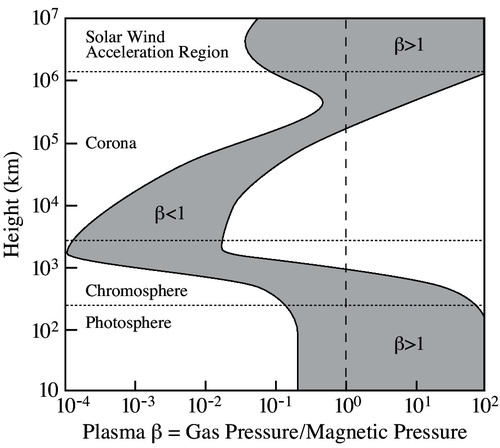
\includegraphics[width = 0.5\textwidth]{figures/introduction/plasma_beta.jpg}
%   \end{center}
%   \vspace{-10pt}
%     % \caption{Courtesy \citet{Gary2001}.}
%      \label{fig:plasma_beta}
% \end{wrapfigure}

Consider the ratio of the pressure force term and Lorentz force term in the momentum equation, Equation \eqref{eq:momentum}, given by
\[\frac{|\grad p|}{|\vec{j}\cross\vec{B}|}\approx \frac{p_0}{B_0^2/\mu}=2\beta,\]
where $p_0$ and $B_0$ denotes the typical size of their respective quantities. The plasma beta, $\beta$, is defined as the ratio of the plasma pressure over the magnetic pressure given by
\begin{equation}
    \label{eq:plasma_beta}
    \beta = \frac{p}{B^2/(2\mu)}.
\end{equation}
Figure \ref{fig:plasma_beta} shows an estimate of the plasma beta as a function of height in the solar atmosphere. It shows that in the solar corona $\beta \ll 1$. Since this Thesis is primarily concerned with modelling waves in the corona, we will often approximate $\beta=0$, which allows us to neglect the pressure force in favour of the Lorentz force.

\begin{figure}
    \centering
    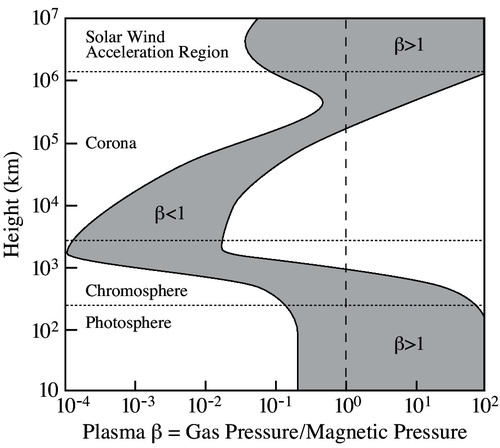
\includegraphics[width = 0.5\textwidth]{figures/introduction/plasma_beta.jpg}
    \caption{The shaded region shows an estimate of the plasma beta in the solar atmosphere as a function of height. This figure was adapted from \citet{Gary2001}.}
    \label{fig:plasma_beta}
\end{figure}

\subsection{Ideal gas law}

For fully ionised Hydrogen plasma the ideal gas law is approximated by
\begin{equation}
    \label{eq:ideal_gas_law}
    p=2\frac{k_B}{m_p}\rho T,
\end{equation}
where $k_B$ denotes the Boltzmann constant approximated by 
\[k_B\approx1.38 \times 10^{-23}\si{.m^2.kg.s^{-2}.K^{-1}}.\]

\subsection{Internal energy equation}
\label{sec:internal_energy_equation}

The most general form of the internal energy equation which we use in this thesis is
\begin{equation}
    \label{eq:internal_energy}
    \pdv{}{t}\qty(\frac{p}{\gamma - 1})+\underbrace{\div(\frac{\gamma p}{\gamma - 1}\vec{v}+\vec{q})}_{\text{Enthalpy flux + Conduction}}=\underbrace{\frac{j^2}{\sigma}+\vec{\sigma}_{Brag}:\grad \vec{v}-n^2Q(T)}_{\text{Ohmic + Viscous heating $-$ Radiation}}.
\end{equation}
The internal energy per unit volume is given by $p/(\gamma - 1)$, where $\gamma$ is the ratio of specific heats, also known as the adiabatic index.

The conduction term is given by the divergence of the heat flux vector, $\vec{q}$. The heat flux vector, $\vec{q}$, is given by
\begin{equation}
    \vec{q}=-\vec{\kappa}\grad T,
\end{equation}
where $\vec{\kappa}$ is the thermal conduction tensor. The divergence of the heat flux may be split into two parts,
\begin{equation}
    \div\vec{q}=\grad_{||}\vdot(\kappa_{||}\grad_{||}T)+\grad_{\perp}(\kappa_\perp\grad_\perp T),
\end{equation}
where $\grad_{||}$ is given by
\begin{equation}
    \grad_{||}=\vec{\hat{B}}(\vec{\hat{B}}\vdot\grad),
\end{equation}
and $\grad_\perp$ is given by
\begin{equation}
    \grad_\perp = \grad - \grad_{||}.
\end{equation}
The thermal conductivity parallel/perpendicular to the field is denoted with $\kappa_{||}$/$\kappa_\perp$ respectively. In coronal plasma, the conductivity is usually much stronger along the field than it is parallel. The parallel conductivity is approximated by
\begin{equation}
    \kappa_{||}=1.8\times10^{-10}\frac{T^{5/2}}{\ln\Lambda}\si{.W.m^{-1}.K^{-1}},
\end{equation}
and the ratio $\kappa_\perp/\kappa_{||}$, for typical coronal parameters, is approximated by
\begin{equation}
    \frac{\kappa_\perp}{\kappa_{||}}=2\times10^{-13}\qty(\frac{n}{10^{15}\si{.m^{-3}}})^2\qty(\frac{10^6\si{.K}}{T})^3\qty(\frac{10^{-3}\si{.T}}{B})^2
\end{equation}
\citep{Spitzer1965, Braginskii1965, Priest2014}. In the corona, the parallel conductivity dominates (except near null points), so we usually neglect the perpendicular conduction.

$Q(T)$ denotes the optically thin radiative loss function. See for example \citet{Rosner1978, Klimchuck2008, Dere2009, Priest2014} for details on the radiative loss function in the solar corona. 
% According to \citet{Klimchuck2008} the radiative loss function, $Q(T)$, is  approximated by (with units $\si{W.m^{3}}$)
% \begin{equation}
% \label{eq:radiative_loss_function}
% Q(T)=\begin{cases}
%     1.09\times10^{-44}T^2, & \text{for } T\le10^{4.97}, \\
%     8.87\times10^{-30}T^{-1}, & \text{for } 10^{4.97}<T\le10^{5.67}, \\
%     1.90\times10^{-35}, & \text{for } 10^{5.67}<T\le10^{6.18}, \\
%     3.53 \times 10^{-26}T^{-3/2}, & \text{for } 10^{6.18}<T\le10^{6.55}, \\
%     3.46 \times 10^{-38}T^{1/3}, & \text{for } 10^{6.55}<T\le10^{6.90}, \\
%     5.49 \times 10^{-29} T^{-1}, & \text{for } 10^{6.90}<T\le10^{7.93}, \\
%     1.96\times 10^{-40} T^{1/2}, & \text{for } 10^{7.93}<T.
% \end{cases}
% \end{equation}
% Note that \citet{Klimchuck2008} gives the radiative losses in units of $\si{erg.s^{-1}.cm^{3}}$ so a conversion factor of $10^{13}$ was used to convert the units into SI base units.
\citet{Klimchuk2015} (and references therein) shows that the temperature evolution of coronal loops is dependent on the time interval, $\Delta t$, between nanoflares/heating events. If the timescale between nanoflares is significantly shorter than the cooling timescale of a loop through conduction and radiation, i.e. $\Delta t \ll \tau_{cool}$, then the temperature evolution can be approximately isothermal (see the left-side of Figure \ref{fig:klimchuck_temperature}). However, if the heating concentrates near the loop footpoints then a loop may be in a state of thermal non-equilibrium, see e.g. \citet{Antiochos2000, Johnston2019}. If the time interval between nanoflares is significantly longer than the cooling timescale, i.e. $\Delta t \gg \tau_{cool}$, then a loop can change in temperature significantly (see the right-side of Figure \ref{fig:klimchuck_temperature}). For simplicity, in this thesis, we will model the plasma as isothermal.

\begin{figure}
    \centering
    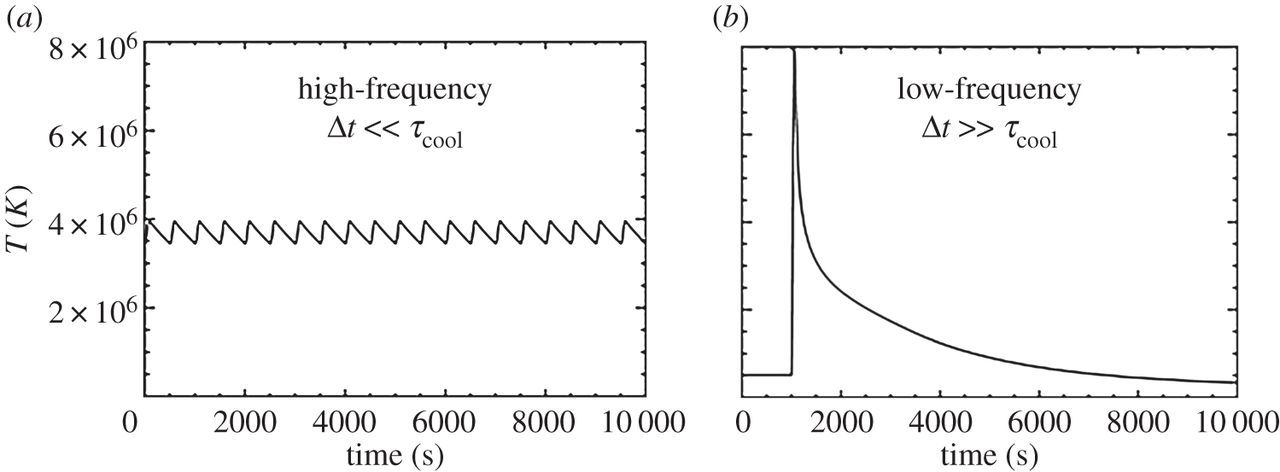
\includegraphics[width=\textwidth]{figures/introduction/klimchuck_temperature.jpg}
    \vspace{-20pt}
    \caption{This figure was taken from \citet{Klimchuk2015}. It shows the temperature evolution in a coronal loop heated by high frequency nanoflares (left) and low-frequency nanoflares (right).}
    \label{fig:klimchuck_temperature}
\end{figure}

% Throughout most of this thesis we model the thermodynamics as adiabatic. In other words, we approximate the internal energy equation as
% \begin{equation}
%     \pdv{}{t}\qty(\frac{p}{\gamma - 1})+\div(\frac{\gamma p}{\gamma - 1}\vec{v})=0.
% \end{equation}
% The Ohmic and viscous heating can be neglected, provided their respective Reynolds numbers satisfy $R_e\gg1$ and $R_m\gg1$ (see Equations \eqref{eq:visc_reynolds_number} and \eqref{eq:mag_reynolds_number}). This thesis is mainly concerned with the evolution of waves. We can neglect conduction and radiation provided the conductive and radiative timescales are much longer than that of a wave period. The timescale at which the pressure changes due to radiation, $\tau_r$, can be approximated by
% \begin{equation}
%     \frac{1}{\gamma - 1}\frac{p_0}{\tau_r}\approx n_0^2Q(T_0),
% \end{equation}
% where $p_0$ denotes the typical pressure in the system $n_0$ denotes the typical number density and $T_0$ denotes the typical temperature. In coronal conditions, with a temperature of $T=10^6\si{.K}$ and an adiabatic index of $\gamma=5/3$, $\tau_r$ can be approximated by
% \begin{equation}
%     \tau_r\approx 0.79\times10^{3}\qty(\frac{p_0}{10^{-2}\si{.Pa}})\qty(\frac{10^{15}}{n_0})^2\si{.s}.
% \end{equation}
% Estimating the conductive timescale is more difficult because it requires knowledge of the temperature length scales which changes by at least an order of magnitude from the corona to the transition region. We can make use of the results from \citet{Withbroe1977} (see Table \ref{tab:energy_loss_fluxes}) to see that the conductive losses are approximately double that of the radiative losses. Hence, in the corona, the timescale of conductive losses, $\tau_c$, is approximately given by
% \begin{equation}
%     \tau_c\approx3.95\times10^2\si{.s}.
% \end{equation}
% These results tell us that conduction and radiation can be neglected for waves with a frequency much greater $10^{-2}\si{.Hz}$.
% A typical coronal loop has a length of say $50\si{.Mm}$ and an Alfv\'en speed of $1\si{.Mm.s^{-1}}$, this gives a fundamental time period of $100\si{s}$. \textcolor{red}{Talk about the Morton power spectrum here, to show the frequencies in which we can ignore. Make your own data and graphs by using the formulas in Paolo's paper. To be honest we can't justify ignoring conduction and radiation. But linear waves do little to affect the density and pressure, so we could simulate it by making our background Alfv\'en speed a function of time.}
% \begin{equation}
%     \frac{1}{\gamma - 1}\frac{p_0}{\tau_c}\approx\frac{\kappa_{||}T_0}{l_0^2},
% \end{equation}
% where $p_0$ denotes the typical pressure in the system, $T_0$ denotes a typical temperature and $l_0$ denotes a typical length-scale for the temperature variations. Hence
% \begin{equation}
%     \tau_c\approx\qty(\frac{p_0}{10^{-2}\si{.Pa}})\qty(\frac{l_0}{10^6\si{.m}})^2\qty(\frac{10^6\si{.K}}{T_0})^{7/2}
% \end{equation}

\subsection{Induction equation}
\label{sec:induction_eqn}

Faraday's law, Equation \eqref{eq:faradays_law}, can be combined with Ohm's law, Equation \eqref{eq:ohms_law}, to give the induction equation,
\begin{equation}
    \label{eq:induction_equation}
    \pdv{\vec{B}}{t}=\underbrace{\curl(\vec{v}\cross\vec{B})}_{\text{Ideal term}}-\underbrace{\curl(\frac{\vec{j}}{\sigma}+\frac{1}{n_ee}\vec{j}\cross\vec{B})}_{\text{Non-ideal term}}.
\end{equation}
If $\vec{j_{||}\gg\vec{j}_\perp}$ then we can neglect the Hall term. Additionally, if we assume that the spatial derivatives of $\sigma$ can be neglected then by using Amp\`ere's law, Equation \eqref{eq:amperes_law} (the induction equation), be written as
\begin{equation}
    \pdv{\vec{B}}{t}=\underbrace{\curl(\vec{v}\cross\vec{B})}_{\text{Advective term}}+\underbrace{\eta\laplacian\vec{B}}_{\text{Diffusive term}},
\end{equation}
where $\eta$ is the magnetic diffusivity, given by
\begin{equation}
    \label{eq:eta_typical_values}
    \begin{aligned}
        \eta&=\frac{1}{\mu_0\sigma} \\
        &\approx 1.09\qty(\frac{T}{10^6\si{.K}})^{-3/2}\si{.m^2.s^{-1}},
    \end{aligned}
\end{equation}
for typical coronal temperatures. The magnetic Reynolds number is defined as
\begin{equation}
    R_m=\frac{l_0V_0}{\eta}\sim\frac{\text{Advective term}}{\text{Diffusive term}},
\end{equation}
where $l_0$ denotes the system's typical length scales and $V_0$ denotes the typical velocity in the system. In the corona, the magnetic Reynolds number can be approximated by
\begin{equation}
    \label{eq:mag_reynolds_number}
    R_m\approx0.95\times10^{10}\qty(\frac{l_0}{10^6\si{.m}})\qty(\frac{V_0}{10^4\si{.m.s^{-1}}})\qty(\frac{T_0}{10^6\si{.K}})^{3/2}.
\end{equation}
We usually neglect the diffusive term in the induction equation in favour of the advective term. However, sometimes the length scales can become sufficiently small that we cannot ignore the diffusion term. Note that our approximation for the corona's velocities uses results from \citet{McIntosh2011,McIntosh2012}.

For typical values, $R_m$, given by Equation \eqref{eq:mag_reynolds_number}, is approximately 8 orders of magnitude larger than $R_e$, given by Equation \eqref{eq:visc_reynolds_number}. This suggests viscous dissipation dominates over resistive. However, this order of magnitude analysis does not consider the fact that gradients perpendicular to the field may be orders of magnitude greater than gradients parallel to the magnetic field. Moreover, there could be significantly more free magnetic energy to dissipate compared with kinetic energy. Note that \citet{vanDoorsselaere2007} uses observations to suggest that resistive heating dominates over viscous.

\subsection{Total energy equation}
\label{sec:intro_total_energy_eqn}

Taking the dot product of Equation \eqref{eq:momentum} with $\vec{v}$ gives
\[\rho\pdv{}{t}\qty(\frac{v^2}{2}) + \rho\vec{v}\cdot\grad(\frac{1}{2}v^2)=\vec{v}\cdot\grad{p} + \vec{v}\cdot(\vec{j}\cross\vec{B}) - \vec{v}\cdot(\rho\grad{\Phi})+\vec{v}\cdot\div{\vec{\sigma}_{Brag}},\]
where $\rho\Phi=\rho g_{\odot}r$ gives the gravitational potential energy density. We can simplify this by using the following identity 
\[\div(\vec{\sigma}_{Brag}\vec{v})=\vec{v}\cdot\div{\vec{\sigma}_{Brag}^T} + \vec{\sigma}_{Brag}:\vec{v},\]
from Equation (1.11.16) of \citet{Kelly2020}, where $\vec{\sigma}_{Brag}:\vec{v}=\tr(\vec{\sigma}_{Brag}\grad{\vec{v}})$ denotes the double-dot product. Note that $\vec{\sigma}_{Brag}$ is symmetric, i.e. $\vec{\sigma}_{Brag}=\vec{\sigma}_{Brag}^T$.
Multiplying Equation \eqref{eq:mass_continuity} with $v^2/2$ gives
\[\frac{v^2}{2}\pdv{\rho}{t}+\frac{v^2}{2}\div(\rho\vec{v})=0.\]
The time-derivative of the gravitational potential energy density gives
\[\pdv{\rho\Phi}{t}=-\Phi\div{\rho\vec{v}}.\]
Combining the above equations gives the equation for the kinetic and gravitational energy,
\[
    \pdv{}{t}\qty(\frac{1}{2}\rho v^2 + \rho\Phi) + \div\qty(\frac{1}{2}\rho v^2\vec{v}+\rho\Phi\vec{v} - \vec{\sigma}_{Brag}\vec{v})=-\vec{v}\cdot\grad{p}+\vec{v}\cdot(\vec{j}\cross\vec{B})-\vec{\sigma}_{Brag}:\vec{v}.
\]

Taking the dot product of Equation \eqref{eq:faradays_law} with $\vec{B}/\mu$ gives
\[\begin{aligned}
\pdv{}{t}\qty(\frac{B^2}{2\mu})&=-\frac{\vec{B}}{\mu}\cdot\curl{\vec{E}} \\
&=-\div(\frac{\vec{E}\cross\vec{B}}{\mu})-\vec{E}\cdot\vec{j}.
\end{aligned}\]
Substituting Equation \eqref{eq:ohms_law} gives the equations for the magnetic energy density,
\[
    \pdv{}{t}\qty(\frac{B^2}{2\mu})+\div(\frac{\vec{E}\cross\vec{B}}{\mu})=-\vec{v}\vdot(\vec{j}\cross\vec{B})-\frac{j^2}{\sigma}.
\]

Therefore the rate of change of total energy is given by
\begin{equation}
    \pdv{}{t}\qty(\frac{1}{2}\rho v^2 + \frac{B^2}{2\mu}+\frac{p}{\gamma-1}+\rho\Phi)+\div{\vec{S}}=-n^2Q(T),
\end{equation}
where
\begin{equation}
    \vec{S} = \frac{1}{2}\rho v^2\vec{v} + \frac{\vec{E}\cross\vec{B}}{\mu} + \frac{\gamma p}{\gamma - 1}\vec{v} + \vec{q} + \rho\Phi\vec{v} - \vec{\sigma}_{Brag}\vec{v}.
\end{equation}

% \section{Our model of a coronal loop}

% This thesis is primarily concerned with the dynamics of waves in coronal loops, like the ones pictured in Figure \ref{fig:coronal_loops_trace}. Throughout this thesis, we study waves by considering perturbations on a background equilibrium. The goal of this section is to provide an overview of our simplest background equilibrium. Our background equilibrium is designed to be as simple as possible, for mathematical convenience, while being complex enough to simulate in a meaningful manner the dynamics of waves in coronal loops. In this section, we aim to clearly show the simplifications which have been made and discuss the likely consequences of these simplifications. We denote background variables with a subscript 0. Later on, in Section \ref{sec:mhd_waves_dispersion_relation}, we will label our perturbed quantities with a subscript 1. Where the time derivatives of the equilibrium quantities are zero.

% Throughout most of this thesis, including this introductory chapter, we model the loops as straight. \textcolor{red}{In chapter X, we look at waves in non-straight magnetic fields}. In other words our background magnetic field, $\vec{B}_0$ given by 
% \begin{equation}
%     \vec{B}_0=B_0\vec{\hat{z}},
% \end{equation}
%, where $B_0$ is a constant and $z$, gives the coordinate along the field. In general, the coronal field is curved, however, the concepts outlined here can still be applied. The effects of loop curvature on coronal kink oscillations are investigated in \citet{vanDoorsselaere2009}. 

% We model our equilibrium as static i.e. $\vec{v}_0=0$ and adiabatic i.e. the internal energy equation is approximated as,
% \begin{equation}
%     \pdv{}{t}\qty(\frac{p}{\gamma - 1})+\div(\frac{\gamma p}{\gamma - 1}\vec{v})=0.
% \end{equation}
% Since the velocity is static and the background field is potential the Ohmic and viscous heating are zero.


% From the mass continuity, Equation \eqref{eq:mass_continuity}, we can see that a static velocity implies that the equilibrium density, $\rho_0$, does not change with time. Moreover, from the induction equation, Equation \eqref{eq:induction_equation}, we can see that the background magnetic field, $\vec{B}_0$, does not change with time. The momentum equation, \eqref{eq:momentum}, shows that for the velocity to remain static, we require
% \begin{equation}
%     \vec{j}_0\cross\vec{B}_0-\grad p_0 - \rho_0 g_\odot\vec{\hat{r}}=0.
% \end{equation}
% Our background field is uniform, therefore, $\vec{j}_0=\vec{0}$. We model the pressure as being in hydrostatic balance, i.e. we assume that
% \begin{equation}
%     \grad p_0 = 
% \end{equation}

% We model the loops as being in thermal equilibrium, i.e. we assume the internal energy does not change with time. This is done for mathematical convenience. See, for example, \citet{Antiochos2000, Johnston2019} for more information on the thermal non-equilibrium in coronal loops. We model the equilibrium temperature and density as not changing with time, therefore, the pressure, $p_0$, does not change with time. Since conduction and radiation are both energy loss mechanisms in the corona, there must be some heating term balancing these losses to maintain thermal equilibrium. We label this coronal heating term $H_c$. Plugging in our equilibrium values into the internal energy equation, Equation \eqref{eq:internal_energy}, with the coronal heating term included, gives
% \begin{equation}
%     \pdv{}{z}\qty(\kappa_{||}\pdv{T_0}{z})+n^2Q(T)=H_c
% \end{equation}

% The coordinate along the loop is $z$. We model the gravity as though the loop were a semi-circle. The gravitational force, $\vec{F}_g$, is given by
% \begin{equation}
%     \vec{F}_g=\sin(\frac{\pi z}{L})g_{\odot}\rho\vec{\hat{z}}.
% \end{equation}
% We assume the loop is in hydrostatic balance.

% Below are listed some of the key assumptions that we make. A diagram of our loop is illustrated in Figure X.
% \begin{enumerate}
%     \item Throughout most of this thesis, including this introductory chapter, we model the loops as straight. \textcolor{red}{In chapter X, we look at waves in non-straight magnetic fields}. In general, the coronal field is curved, however, the concepts outlined here can still be applied. We model the gravity as though the loop were a semi-circle. The gravitational force, $\vec{F}_g$, is given by
%     \begin{equation}
%         \vec{F}_g=\sin(\frac{\pi z}{L})g_{\odot}\rho\vec{\hat{z}}
%     \end{equation}
%     \item We approximate the transition region as a discontinuity. This means that we model the temperature, density and pressure as being discontinuous at the transition region.  When studying waves, the transition region can be approximated as a discontinuity provided the wavelength of the wave is longer than the width of the transition region.
%     \item We model the temperature in the corona as isothermal. In reality, the temperature of a typical coronal loop increases with height. We model our equilibrium as being in hydrostatic balance and so by assuming isothermal temperature this means we are overestimating the scale height of the density.
% \end{enumerate}

\section{MHD waves: Dispersion relation}
\label{sec:mhd_waves_dispersion_relation}

Solving the MHD equations is notoriously difficult. Some of the basic properties of the Navier-Stokes equations, which is a subset of the MHD equations, are not known. There is a famous problem known as the Navier–Stokes existence and smoothness problem. The Clay Mathematics Institute in May 2000 made this problem one of its seven Millennium Prize problems in mathematics. It offered a \$1,000,000 prize to the first person to solve the problem. The challenge is to prove or give a counter-example of the following statement:
\begin{displayquote}
In three space dimensions and time, given an initial velocity field, there exists a vector velocity and a scalar pressure field, which are both smooth and globally defined, that solve the Navier–Stokes equations.
\end{displayquote}

Due to the difficulty in solving the MHD equations, solutions are usually calculated numerically. To obtain an analytic solution, we study a simplified plasma. Analytical solutions are useful as a starting point for understanding plasma dynamics. Moreover, parameters can be arbitrary constants which allows a large parameter space to be studied simultaneously. Typically, numerical simulations only calculate the solution for a single set of parameters, and then the simulation has to be restarted if different parameters wish to be studied.

Given that the corona has a large Reynolds number (see Equations \ref{eq:visc_reynolds_number} and \ref{eq:mag_reynolds_number}) we model the plasma as ideal. Additionally, the plasma beta in the corona is small (see Figure \ref{fig:plasma_beta}) so we assume the only force in the momentum equation is the Lorentz force. This gives the momentum equation as
\begin{equation}
    \label{eq:momentum_eqn_beta=0}
    \rho\frac{D \vec{v}}{D t}=\frac{1}{\mu}(\curl{\vec{B}})\cross\vec{B},
\end{equation}
the induction equation as
\begin{equation}
    \label{eq:induction_eqn_ideal}
    \pdv{\vec{B}}{t}=\curl(\vec{v}\cross\vec{B}),
\end{equation}
and mass continuity equation as,
\begin{equation}
    \tag{\ref{eq:mass_continuity}}
    \pdv{\rho}{t}+\div(\rho\vec{v})=0.
\end{equation}
Finally, we model the plasma as isothermal, see Section \ref{sec:internal_energy_equation},
\begin{equation}
    T = T_0(\vec{x}),
\end{equation}
note that the pressure can be calculated from the ideal gas law, Equation \eqref{eq:ideal_gas_law}.

We model small perturbations on a static background equilibrium in other words we assume
\begin{gather}
    \label{eq:linear_assumotion_v}
    \vec{v}(\vec{x},t) = \vec{u}(\vec{x},t),\ \text{where}\ u\ll v_A,\\
    \label{eq:linear_assumotion_b}
    \vec{B}(\vec{x},t) = \vec{B}_0(\vec{x}) + \vec{b}(\vec{x},t),\ \text{where}\ b\ll B_0, \\
    \label{eq:linear_assumotion_rho}
    \rho(\vec{x},t) = \rho_0(\vec{x}) + \rho_1(\vec{x},t),\ \text{where}\ \rho_1\ll \rho_0,
\end{gather}
where
\[u = \abs{\vec{v}},\ B_0=\abs{\vec{B}_0}\ ,b=\abs{\vec{b}}.\] Note that $\vec{B}_0$ and $\rho_0$ are referred to as the background quantities which are specified beforehand and $\vec{v}$, $\vec{b}$ and $\rho_1$ are the perturbed quantities which need to be calculated.
We assume $u\ll v_A$ because observations suggest $u / v_A$ to be approximately in the range [$10^{-2}$,\ $10^{-1}$] \citep{McIntosh2011,McIntosh2012}. We approximate $\pdv*{B_0}{t}=0$ since magnetic structures can last much longer than the typical frequency and Alfv\'en travel time of waves in a coronal loop. If we take the Alfv\'en speed in the corona as about $1\si{.Mm.s^{-1}}$ \citep{McIntosh2011} and assume that coronal loops have a characteristic length of about 100$\si{.Mm}$ \citep{O'Neill2005} then This gives an Alfv\'en travel time of about $100\si{.s}$. Magnetic structures can last much longer than this, for example, active region prominences can last a few hours or a day, while quiescent prominences can last between a few and 300 days \citep{Priest2014}. We assume $\pdv*{\rho_0}{t}=0$ and this explains why we model the plasma as isothermal since temperature changes as large at those shown on the right-side of Figure \ref{fig:klimchuck_temperature} will in general also corresponds to similarly large changes in the density (assuming the pressure is approximately constant in time).
% We will see in \textcolor{red}{Equation X} that provided
% \[f\gg \frac{\langle v_A \rangle}{L},\]
% then
% \[\frac{b}{\sqrt{\mu}}\sim \sqrt{\rho}u,\]
% where $f$ denotes the frequency of the wave, $\langle v_A \rangle$ denotes the average Alfv\'en speed along the length of a loop and $L$ denotes the length of the loop. Hence, if $u\ll v_A$ then this implies that $b\ll B_0$. \textcolor{red}{Note that typical values for L vA and f are THIS and we typically study waves with frequencies greater than.} Note that if 
% \[f\ll \frac{\langle v_A \rangle}{L},\]
% then it is possible for
% \[\frac{b}{\sqrt{\mu}}\gg \sqrt{\rho}u.\]
% We justify, in part, the assumption given by Equation \eqref{eq:linear_assumotion_rho} by modelling the plasma as isothermal. Therefore, provided the background pressure, $p_0$, remains constant, then by the ideal gas law, Equation \eqref{eq:ideal_gas_law}, the background density, $\rho_0$, must also remain constant is perhaps the hardest to justify. In Section \ref{sec:internal_energy_equation} we showed that conduction and radiation can lead to changes in the plasma pressure and density in a timescale, $\tau_c$, which is comparable to that of typical wave frequencies we will be studying. Moreover, research has shown that loops are typically in a state of thermal nonequilibrium and this can lead to the density growing or shrinking by a factor greater than 2 over a timescale $\tau_c$ \citep{Antiochos2000, Johnston2020}. However, modelling the background density, $\rho_0$ as static is a useful place to start to build our intuition. Future research will look at waves in a domain where the background density evolves with time.

The final assumption we make, in this section, is to assume the background quantities are uniform, primarily because this allows the equations to be solved analytically more easily. Without loss of generality, we can model the background magnetic field as being directed in the $z$-direction, i.e.
\begin{equation}
    \label{eq:background_field}
    \vec{B}_0=B_0\vec{\hat{z}}.
\end{equation}
With these assumptions in place we can simplify Equation \eqref{eq:momentum_eqn_beta=0} and \eqref{eq:induction_eqn_ideal} via a linearization procedure. This is where we neglect terms involving the product of small terms i.e. $\vec{u}$, $\vec{b}$ or $\rho_1$ and neglect the time-derivatives of the background terms $\vec{B}_0$, $\rho_0$. The momentum equation reduces to
\begin{equation}
    \label{eq:momentum_eqn_linear}
    \begin{aligned}
        \pdv{\vec{u}}{t}&=\frac{1}{\mu\rho_0}(\curl{\vec{b}})\cross\vec{B}_0 \\
        &=\frac{B_0}{\mu\rho_0}\qty[(\vec{B}_0\cdot\grad)\vec{b} - \grad\qty(\frac{\vec{b}\cdot\vec{B}_0}{2\mu})].
    \end{aligned}
\end{equation}
The induction equation simplifies to
\begin{equation}
    \begin{aligned}
    \pdv{\vec{b}}{t}&=\curl(\vec{u}\cross\vec{B}_0) \\
    &=(\vec{B}_0\cdot\grad)\vec{u} - \vec{B}_0\div{\vec{u}},
    \end{aligned}
\end{equation}
and the mass continuity equation is given by
\begin{equation}
    \pdv{\rho_1}{t}+\div(\rho_0\vec{v})=0.
\end{equation}
Note that $\vec{u}$ and $\vec{b}$ are independent of $\rho_1$ and so we only need to solve for $\vec{u}$ and $\vec{b}$.
Written out component-wise the above equations become
\begin{gather}
    \pdv{u_x}{t} = v_{A0}^2\qty[\pdv{\hat{b}_x}{z} - \pdv{\hat{b}_z}{x}],\\
    \label{eq:uy_eqn_linear}
    \pdv{u_y}{t} = v_{A0}^2\qty[\pdv{\hat{b}_y}{z} - \pdv{\hat{b}_z}{y}],\\
    \label{eq:bx_eqn_linear}
    \pdv{\hat{b}_x}{t} = \pdv{u_x}{z},\\
    \label{eq:by_eqn_linear}
    \pdv{\hat{b}_y}{t} = \pdv{u_y}{z},\\
    \pdv{\hat{b}_z}{t} = -\qty[\pdv{u_x}{x} + \pdv{u_y}{y}],
\end{gather}
where
\begin{gather}
    \label{eq:b_hat}
    \vec{\hat{b}}=\frac{\vec{b}}{B_0}=(\hat{b}_x,\hat{b}_y,\hat{b}_z),\\
    v_{A0} = \frac{B_0}{\sqrt{\mu\rho_0}}.
\end{gather}
Since the Lorentz force is perpendicular to the background field, $u_z$, is is decoupled from the and can be treated separately. We can eliminate $\hat{b}_x$ and $\hat{b}_y$ from the above equations to give
\begin{gather}
    \label{eq:ux_in_terms_of_bz}
   \qty(\pdv[2]{}{t}-v_{A0}^2\pdv[2]{}{z})u_x=-v_{A0}^2\pdv{\hat{b}_z}{x}{t}, \\
    \label{eq:uy_in_terms_of_bz}
   \qty(\pdv[2]{}{t}-v_{A0}^2\pdv[2]{}{z})u_y=-v_{A0}^2\pdv{\hat{b}_z}{y}{t}.
\end{gather}
Eliminating $\hat{b}_z$ gives
\begin{gather}
   \qty[\pdv[2]{}{t}-v_{A0}^2\qty(\pdv[2]{}{x}+\pdv[2]{}{z})]u_x=v_{A0}^2\pdv{u_y}{x}{y}, \\
    \label{eq:uy_in_terms_of_ux}
   \qty[\pdv[2]{}{t}-v_{A0}^2\qty(\pdv[2]{y}+\pdv[2]{}{z})]u_y=v_{A0}^2\pdv{u_x}{x}{y}.
\end{gather}
Eliminating $u_y$ gives
\[\qty[\pdv[2]{}{t}-v_{A0}^2\qty(\pdv[2]{y}+\pdv[2]{}{z})]\qty[\pdv[2]{}{t}-v_{A0}^2\qty(\pdv[2]{}{x}+\pdv[2]{}{z})]u_x=v_{A0}^4\frac{\partial^4 u_x}{\partial x^2 \partial y^2},\]
\[\begin{aligned}
\implies &\qty[\pdv[2]{}{t}-v_{A0}^2\pdv[2]{}{z}]\qty[\pdv[2]{}{t}-v_{A0}^2\qty(\pdv[2]{}{x}+\pdv[2]{}{z})]u_x=\\
&v_{A0}^2\pdv[2]{}{y}\qty{v_{A0}^2\pdv[2]{}{x}+\qty[\pdv[2]{}{t}-v_{A0}^2\qty(\pdv[2]{}{x}+\pdv[2]{}{z})]}u_x,
\end{aligned}\]
hence
\begin{equation}
    \implies \qty[\pdv[2]{}{t}-v_{A0}^2\pdv[2]{}{z}]\qty[\pdv[2]{}{t}-v_{A0}^2\qty(\pdv[2]{}{x}+\pdv[2]{}{y}+\pdv[2]{}{z})]u_x=0.
\end{equation}
Since all the coefficients are constant we can use a useful trick to calculate an analytic solution which satisfies the above equation. We assume $u_x$ is of the form
\[u_x = u_{x0}\exp[i(k_x x + k_y y + k_z z + \omega_n t)],\]
where $k_x$, $k_y$, $k_z$ and $\omega_n$ $\in \mathds{C}$.
and this reduces our PDE to the following algebraic equation
\begin{equation}
    [\omega_n^2 - v_{A0}^2k_z^2][\omega_n^2 - v_{A0}^2(k_x^2+k_y^2+k_z^2)] = 0.
\end{equation}
The above dispersion equation shows that four types of solution can exist. The solutions are given by
\[\omega_1 = v_{A0}k_z,\]
\[\omega_2 = -v_{A0}k_z,\]
\[\omega_3 = v_{A0}\sqrt{k_x^2 + k_y^2 + k_z^2},\]
\[\omega_4 = -v_{A0}\sqrt{k_x^2 + k_y^2 + k_z^2}.\]
Solutions where $\omega = \omega_1$ or $\omega_2$ are called Alfv\'en wave solutions and solutions where $\omega = \omega_3$ or $\omega_4$ are fast wave solutions. The next two subsections go into further detail about each wave, respectively.

For now, we calculate the solution for case where the perturbed quantities, $u_x$, $u_y$, $\hat{b}_x$, $\hat{b}_y$ and $\hat{b}_z$ have an $x$, $y$, $z$ and $t$ dependence of the form
\[f(x,y,z,t)=f_0\exp[i(k_xx + k_y y + k_z z + \omega_n t)],\]
where
\[\omega = \pm v_{A0}k_z.\]
Let $u_{x0}$ be fixed, from Equation \eqref{eq:uy_in_terms_of_ux} we know that
\begin{equation}
    \label{eq:uy0}
    u_{y0} = \frac{v_{A0}^2 k_x k_y}{\omega^2 - v_{A0}^2(k_y^2 + k_z^2)}u_{x0}.
\end{equation}
From Equations \eqref{eq:bx_eqn_linear} and \eqref{eq:by_eqn_linear} we know that
\begin{gather}
    \label{eq:bx0}
    \hat{b}_{x0} = \frac{k_z}{\omega}u_{x0}, \\
    \label{eq:by0}
    \hat{b}_{y0} = \frac{k_z}{\omega}u_{y0}.
\end{gather}
From Equation \eqref{eq:ux_in_terms_of_bz} we know that
\begin{equation}
    \label{eq:bz0}
    \hat{b}_z = -\frac{\omega^2 - v_{A0}^2k_z^2}{k_x \omega} u_{x0}.
\end{equation}


\subsection{Alfv\'en waves}

We define Alfv\'en waves \citep{Alfven1942} as waves with a velocity amplitude, $\vec{u}$, which satisfy the Alfv\'en wave equation, which is given by
\begin{equation}
    \label{eq:alfven_wave_equation}
    \mathcal{L}\vec{u} = \qty(\pdv[2]{}{t} - \frac{1}{\mu\rho}(\vec{B}_0\cdot\grad)^2)\vec{u}=0,
\end{equation}
where $\mathcal{L}$ denotes the Alfv\'en wave equation operator and $\vec{B}_0$ denotes the background magnetic field. This shows that Alfv\'en waves propagate parallel to the background magnetic field with speed given by the Alf\'en speed. Note that for our configuration above the Alfv\'en wave equation operator, $\mathcal{L}$, becomes
\begin{equation}
    \label{eq:alfven_wave_equation_operator}
    \mathcal{L} = \pdv[2]{}{t} - v_{A0}\pdv[2]{}{z}.
\end{equation}
Equations \eqref{eq:ux_in_terms_of_bz} and \eqref{eq:uy_in_terms_of_bz} show that if $\mathcal{L}u_x=\mathcal{L}u_y=0$ then $b_z=b_z(z)$. Therefore, applying the initial condition that $b_z$ is initially zero ensures $b_z=0$ $\forall t$. Note that $b_z$ gives the perturbation in magnetic pressure. For this reason, Alfv\'en waves can be thought of as kinetic-tension waves as they are an oscillation in kinetic and magnetic tension energy. Very much like waves on a guitar string but with magnetic tension replaced with tension in the string.

% A useful quantity is the Poynting flux, $\vec{S}$ given by
% \begin{equation}
%     \label{eq:poynting_flux}
%     \begin{aligned}
%     \vec{S}&=\frac{\vec{E}\times\vec{b}}{\mu} \\
%     & = \frac{1}{\mu}\qty[(\vec{B}_0\cdot\vec{b})\vec{u}-(\vec{u}\cdot\vec{b})\vec{B}_0].
%     \end{aligned}
% \end{equation}
% where $\vec{E}$ denotes the electric field and we approximate it by linearizing Ohm's law (Equation \eqref{eq:ohms_law}) and assuming ideal MHD to give
% \begin{equation}
%     \vec{E}=-\vec{u}\times\vec{B}_0.
% \end{equation}
% This gives the directional energy flux, to see this consider the following.
% Taking the dot product of Equation \eqref{eq:momentum_eqn_linear} with $\rho_0 \vec{u}$ gives
% \[\pdv{}{t}\left(\frac{1}{2}\rho_0 u^2\right)=\frac{1}{\mu}\vec{u}\cdot\qty[(\vec{B}_0\cdot\vec{\nabla})\vec{b}-\vec{\nabla}(\vec{B}_0\cdot\vec{b})].\]
% Taking the dot product of Equation \eqref{eq:induction_eqn_ideal} with $\vec{b}$ gives
% \[\pdv{}{t}\left(\frac{b^2}{2\mu}\right)=\frac{1}{\mu}\vec{b}\cdot\qty[(\vec{B}_0\cdot\vec{\nabla})\vec{u}-\vec{B}_0(\div\vec{u})].\]
% Note that
% \[\pdv{}{t}\qty(\frac{1}{2}\rho_0 u^2 + \frac{b^2}{2\mu})=-\frac{1}{\mu}\div\qty[(\vec{B}_0\cdot\vec{b})\vec{u} - (\vec{u}\cdot\vec{b})\vec{B}_0],\]
% Hence, the energy equation is given by
% \begin{equation}
%     \pdv{}{t}\qty(\frac{1}{2}\rho u^2+\frac{b^2}{2\mu}) + \div{\vec{S}}=0.
% \end{equation}
% This confirms that $\vec{S}$ does indeed give the energy flux for the magnetic and kinetic energy. For Alfv\'en waves, the magnetic pressure perturbation is zero, therefore, the Poytning flux is directed along the magnetic field (see Equation \eqref{eq:poynting_flux}). This means that Alfv\'en waves can only propagate parallel to the magnetic field.

Note that if $\omega=\pm k_z v_A$ then Equations \eqref{eq:uy0}-\eqref{eq:bz0} simplify to
\begin{gather}
    \label{eq:uy0_alfven}
    u_{y0} = -\frac{k_x}{k_y}u_{x0}, \\
    \hat{b}_{x0} = \pm \frac{u_{x0}}{v_{A0}}, \\
    \hat{b}_{y0} = \pm \frac{u_{y0}}{v_{A0}}, \\
    \hat{b}_{z0} = 0.
\end{gather}
This shows that the magnetic pressure perturbation is zero and so all the energy is contained within the magnetic tension.

\subsection{Fast waves}

We define fast waves in $\beta=0$ plasma as waves with velocity amplitude, $\vec{u}$, which satisfy the classical wave equation,
\begin{equation}
    \qty(\pdv[2]{}{t}+v_A^2\laplacian)\vec{u}=0.
\end{equation}
This shows that fast waves propagate isotropically with a speed given by the Alfv\'en speed.
Note that this is only valid for $\beta=0$ plasma, for $\beta\ll 1$ then the fast wave propagates perpendicular to the field at a speed of approximately $v_A + c_s$ and parallel to the field at a speed of $v_A$, where $c_s$ gives the background sound speed. For a derivation of the dispersion relation of fast waves (and its sibling slow waves) in a $\beta>0$ plasma, see for example \citet{Priest2014, Roberts2019}.
 

Note that if $\omega=\pm v_{A0}\sqrt{k_x^2 + k_y^2 + k_z^2}$, then Equations \eqref{eq:uy0}-\eqref{eq:bz0} simplify to
\begin{gather}
    \label{eq:uy0_fast}
    u_{y0}=\frac{k_y}{k_x}u_{x0}, \\
    \label{eq:bx0_fast}
    \hat{b}_{x0} = \frac{k_z}{\sqrt{k_x^2 + k_y^2 + k_z^2}}\frac{u_{x0}}{v_{A0}}, \\
    \label{eq:by0_fast}
    \hat{b}_{y0} = \frac{k_z}{\sqrt{k_x^2 + k_y^2 + k_z^2}}\frac{u_{y0}}{v_{A0}}, \\
    \label{eq:bz0_fast}
    \hat{b}_{z0} = -\frac{k_x^2+k_y^2}{k_x\sqrt{k_x^2 + k_y^2 + k_z^2}}\frac{u_{x0}}{v_{A0}},
\end{gather}
The above equation shows that, unlike Alfv\'en waves, the magnetic pressure perturbation, $b_z$, is in general non-zero. Fast waves are oscillations in kinetic and magnetic energy, where the restoring force can be magnetic tension and the magnetic pressure. More generally, in a $\beta>0$ plasma, the plasma pressure also acts as a restoring force and contributes towards the energy associated with the fast wave.

\subsection{Poynting flux}

The Poynting flux, $\vec{S}$ is given by
\begin{equation}
    \label{eq:poynting_flux_linear}
    \begin{aligned}
    \vec{S}&=\frac{\vec{E}\times\vec{b}}{\mu} \\
    & = \frac{1}{\mu}\qty[(\vec{B}_0\cdot\vec{b})\vec{u}-(\vec{u}\cdot\vec{b})\vec{B}_0].
    \end{aligned}
\end{equation}
where $\vec{E}$ denotes the electric field and we approximate it by linearizing Ohm's law (Equation \eqref{eq:ohms_law}) and assuming ideal MHD to give
\begin{equation}
    \label{eq:ideal_linear_ohms_law}
    \vec{E}=-\vec{u}\times\vec{B}_0.
\end{equation}
$\vec{S}$ gives the directional energy flux, to see this consider the following.
Taking the dot product of Equation \eqref{eq:momentum_eqn_linear} with $\rho_0 \vec{u}$ gives
\[\pdv{}{t}\left(\frac{1}{2}\rho_0 u^2\right)=\frac{1}{\mu}\vec{u}\cdot\qty[(\vec{B}_0\cdot\vec{\nabla})\vec{b}-\vec{\nabla}(\vec{B}_0\cdot\vec{b})].\]
Taking the dot product of Equation \eqref{eq:induction_eqn_ideal} with $\vec{b}$ gives
\[\pdv{}{t}\left(\frac{b^2}{2\mu}\right)=\frac{1}{\mu}\vec{b}\cdot\qty[(\vec{B}_0\cdot\vec{\nabla})\vec{u}-\vec{B}_0(\div\vec{u})].\]
Note that
\[\pdv{}{t}\qty(\frac{1}{2}\rho_0 u^2 + \frac{b^2}{2\mu})=-\frac{1}{\mu}\div\qty[(\vec{B}_0\cdot\vec{b})\vec{u} - (\vec{u}\cdot\vec{b})\vec{B}_0],\]
Hence, the energy equation is given by
\begin{equation}
    \label{eq:total_energy_eqn_linear}
    \pdv{}{t}\qty(\frac{1}{2}\rho u^2+\frac{b^2}{2\mu}) + \div{\vec{S}}=0.
\end{equation}
This confirms that $\vec{S}$ does indeed give the energy flux for the magnetic and kinetic energy. For Alfv\'en waves, the magnetic pressure perturbation is zero. Therefore, the Poynting flux points along the magnetic field (see Equation \eqref{eq:poynting_flux_linear}).


\section{MHD waves: power spectrum}
\label{sec:mhd_waves_power_spectrum}

MHD waves are ubiquitous and have been observed in for example \citet{Tomczyk2007,McIntosh2011,DeMoortel2012}. These observations are useful for constraining theoretical models and may help answer unsolved problems such as the coronal heating problem. Measurements of the waves' amplitude and wavelength could play an important role in deciding whether MHD waves play an essential or negligible role in coronal heating. Note that the Ohmic and viscous heat provided by MHD waves typically increases with larger wave amplitudes and shorter wavelengths.  A power spectrum can represent the wave amplitude and frequency. This section aims to give a brief overview of the power spectrum of velocity fluctuations in the corona and explain how we calculate it.

In for example \citet{Morton2016,Morton2019}, the power spectrum of velocity fluctuations in the solar corona is calculated. They produce a time sequence, $\{v_n\}$, of the Doppler velocities on the limb of the corona using data from the Coronal Multi-channel Polarimeter (CoMP). CoMP only has a finite cadence and they can only observe the fluctuations for a finite time. Therefore, the observed velocities, $\{v_n\}$, can only be measured at a finite discrete sequence of times $\{t_n\}$. If $N$ measurements are made, i.e.
\[\{v_n\}=v_0, v_1, ... v_{N-1},\]
then we can write 
\[\begin{aligned}
v_n &= \frac{1}{N}\sum_{k=0}^{N-1}V_k\exp(2i\pi  k n / N) \\
&= \frac{1}{N}\sum_{k=0}^{N-1}V_k\exp(2i\pi f_k t_n),
\end{aligned}\]
where
\[t_n = n\Delta t,\]
\[f_k = \frac{k}{N \Delta t},\]
and $\{V_k\}$ is the discrete Fourier transform of $\{v_n\}$, given by
\[\begin{aligned}
V_k&=\sum_{n=0}^{N-1}v_n\exp(-2i\pi k n / N) \\
&=\sum_{n=0}^{N-1}v_n\exp(-2i\pi f_k t_n).
\end{aligned}\]
Note that a measure of the average energy associated with the velocity fluctuations is given by
\begin{equation}
    \langle v^2 \rangle = \frac{1}{N}\sum_{n=0}^{N-1}v_n^2.
\end{equation}
By the Plancheral theorem
\begin{equation}
    \langle v^2 \rangle = \frac{1}{N^2}\sum_{k=0}^{N-1}|V_k|^2.
\end{equation}
Therefore, $|V_k|^2/N^2$ gives a useful measure of the average energy associated with each frequency, $f_k$, for the signal, $\{v_n\}$. Note that $|V_k|$ is Hermitian-symmetric because $\{v_n\}$ is strictly real, i.e.
\begin{equation}
    V_k = \bar{V}_{N-k},\quad \text{for}\ 1 \le k\le N-1,
\end{equation}
% where
% \begin{equation}
%     N_{mid} = \begin{cases}
%     N / 2 - 1, & \text{for}\ N\ \text{even}, \\
%     (N - 1) / 2, & \text{for}\ N\ \text{odd},
%     \end{cases}
% \end{equation}
where $\bar{V}_{N-k}$ denotes the complex conjugate and $\lfloor\,\rfloor$ denotes the floor function which rounds down to the nearest integer. Therefore, we define the power spectrum, $P_k[\{v_n\}]$, as
\begin{equation}
    \label{eq:discrete_power_spectrum_definition}
    P_k[\{v_n\}] = \frac{1}{N^2}\begin{cases}
    |V_0|^2, & \text{for}\ k=0,\\
    |V_k|^2, & \text{for}\ k=N/2\ \text{and}\ N\ \text{even},\\
    2|V_k|^2, & \text{otherwise},\\
    \end{cases}
\end{equation}
where $k=0,1...,\lfloor N / 2\rfloor$. This ensures that $P_k[\{v_n\}]$ satisfies
\begin{equation}
    \langle v^2 \rangle = \sum_{k=0}^{\lfloor N / 2 \rfloor}P_k[\{v_n\}].
\end{equation}

\begin{figure}
    \vspace{-20pt}
    \centering
    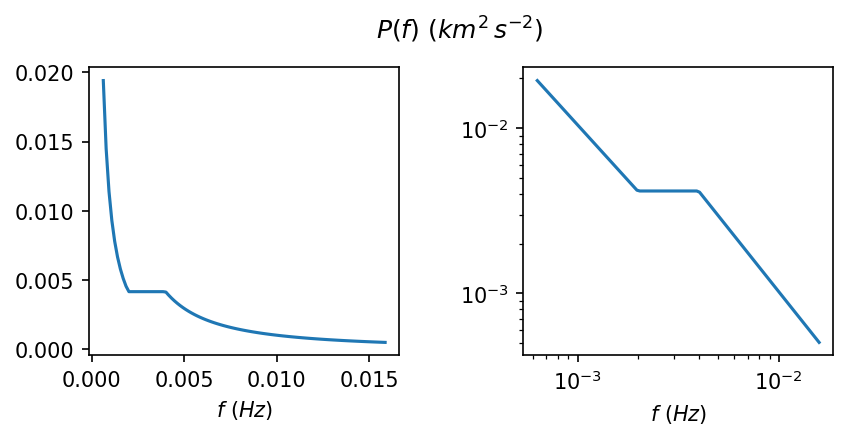
\includegraphics[width=\textwidth]{figures/introduction/power_spectrum_morton.png}
    \vspace{-35pt}
    \caption{This figure shows the approximate power spectrum for velocity fluctuations in the corona using data from \citet{Morton2016} and an approximation used in \citet{Pagano2019}. The left-hand side uses a linear axis while the right-hand side uses a log-log axis. The code used to make this figure is available on GitHub in the following directory:\newline
    \href{https://github.com/aleksyprok/apkp_thesis/blob/main/Python/Introduction/power_spectrum.py}{$\rightarrow$ Python/Introduction/power\_spectrum.py}}
    \vspace{-10pt}
    \label{fig:power_spectrum_morton}
\end{figure}

To plot the average power spectrum, $P(f)=P_k[\{v_n\}]$, we will use an approximation given in \citet{Pagano2019} which uses data from \citet{Morton2016}. They state that the power spectrum in $\si{km^2.s^{-2}}$ can be approximated as
\begin{equation}
    P(f) = \begin{cases}
    10^{-6}f^{-1.34},     & 10^{-3.2} \le f \le 10^{-2.7}, \\
    10^{-2.38},           & 10^{-2.7} \le f \le 10^{-2.4}, \\
    10^{-6.05}f^{-1.53}, & 10^{-2.4} \le f \le 10^{-1.8}, \\
    \end{cases}
\end{equation}
where the frequency is measured in $\si{Hz}$. 
Note that the dimensions of $P(f)$ are somewhat meaningless without knowledge of the number of points used, however, for now, we are only interested in the shape of the power spectrum. \cite{McIntosh2011,McIntosh2012}  measured the average amplitude of velocity fluctuations in the corona. They show that observed amplitudes are of the order 10$\si{.km.s^{-1}}$. $P(f)$ is plotted in Figure \ref{fig:power_spectrum_morton}. We can only plot the power spectrum for a finite range of frequencies because the equipment’s cadence is limited. Moreover, we can only observe features for about half a solar rotation before moving out of view. Here the frequency range is $10^{-3.2}\si{.Hz} \le f \le 10^{-1.8}\si{.Hz}$. \citet{Podesta2007} can observe higher frequency waves have in the solar wind.

\section{Outline of the thesis}

This thesis aims to model MHD waves' dynamics in the solar atmosphere by using simple models to calculate analytic solutions. In Chapter \ref{chap:ideal_footpoint_driven_alfven_waves} we study the simplest type of MHD wave, namely, Alfv\'en waves. These are waves with a velocity amplitude which satisfies the Alfv\'en wave equation, Equation \eqref{eq:alfven_wave_equation}. We calculate the solutions for the case where we impose a footpoint driver as a boundary condition. We aim to show how to set up resonance when the driver is sinusoidal and gives a white/red noise force. We also consider the case where waves can leak out of the corona.

In Chapter \ref{chap:resistive_phase_mixed_alfven_waves} we study linear Alfv\'en waves with resistivity and viscosity included in the model with the $y$-direction assumed invariant. We show that if neighbouring field lines have different natural frequencies, this can lead to the formation of steep gradients across the field via phase mixing. We aim to test if the dissipation of phase-mixed Alfv\'en waves plays a significant role in coronal heating. To do this, we introduce a quantity called the heating rate per unit of wave energy which we denote with $\gamma$. We estimate the required heating rate by assuming it must balance our estimates of the corona's conductive and radiative losses. We also use observational data of velocity fluctuations to estimate the average wave energy in the corona. Using these values, we calculate that $\gamma$ needs to equal about $10^{-1}\si{.s^{-1}}$ for a wave heating mechanism to play a major role in coronal heating. We calculate a theoretical upper bound for $\gamma$ and use this to test if the dissipation of phase-mixed Alfv\'en wave is a viable heating mechanism. Our model also includes partial reflection and allows for a power spectrum of harmonics to be excited.

Chapter \ref{chap:resonant_absorption_in_an_oblique_field} allows for $\pdv*{}{y}\ne0$. This enables a phenomenon called resonant absorption to occur. This is where a propagating fast wave with a given frequency gets absorbed by a magnetic field line, called the resonant field line, with the same natural Alfv\'en frequency. Energy concentrates at the resonant field line and the waves form a standing Alfv\'en wave. We model the magnetic field to be at an arbitrary angle, $\alpha$, to the transition region. In for example, \citet{Halberstadt1993,Halberstadt1995,Arregui2003}, they show that in general, steep boundary layers / evanescent fast waves form. However, their model only includes the corona, and they impose line-tied boundary conditions. This chapter includes the chromosphere and corona and tests if the boundary layers still form if we do not impose line-tied boundary conditions. This allows us to test if the boundary layers are physical or fictitious artefacts generated by using line-tied boundary conditions.

Finally, in Chapter \ref{chap:conclusions_and_future_work} a summary of results from each of the chapters is given, and we discuss ideas for further study.

\chapter{Ideal footpoint driven Alfv\'en waves}
\label{chap:ideal_footpoint_driven_alfven_waves}
\section{Introduction}

Before we can discuss the results from our more technical research in Chapters \ref{chap:resistive_phase_mixed_alfven_waves} and \ref{chap:resonant_absorption_in_an_oblique_field} we need to first understand the dynamics of waves in a more simple domain.
This chapter models footpoint driven linear Alfv\'en waves in a uniform domain to establish some of the key ideas we will use throughout this thesis.
We will see in Chapter \ref{chap:resistive_phase_mixed_alfven_waves} that if an invariant direction is assumed, in this case, $\pdv*{}{y}=0$, then the velocity perturbations in the invariant direction (in this case, $v_y$), must satisfy the Alfv\'en wave equation. Chapter \ref{chap:resonant_absorption_in_an_oblique_field} shows that propagating fast waves with a given frequency will mode convert at a field line with the same natural frequency to form standing Alfv\'en waves. This phenomenon is called resonant absorption. Moreover, a similar effect was demonstrated in more general three-dimensional domains (see for example, \citealt{Wright2016,Elsden2017,Elsden2018}). This suggests that Alfv\'en waves and approximate Alfv\'en waves are ubiquitous throughout the solar atmosphere.

The outline of this chapter is as follows. 
In Section \ref{sec:chap_2_model_and_equations} we introduce the model we use and discuss the assumptions we will make. In Sections \ref{sec:chap_2_closed_loop_general_soln}-\ref{sec:closed_loop_sinusoidal_solution} we calculate the solution for a closed loop with a footpoint driver. We show how a footpoint driver can excite resonances along the loop. We will calculate the solutions for the case where the driver is sinusoidal and excites resonant frequencies, nearly resonant frequencies and frequencies halfway in between different resonant frequencies.
After that, in Section \ref{sec:closed_loop_random_driver}, we will study the solution when we use a noisy driver. We think of a noisy driver as a superposition of an infinite number of sinusoidal drivers. We use a white and red noise force driver where the slope of its power spectrum defines the noise's colour, and this is explained further in Section \ref{sec:closed_loop_random_driver}. One of the goals in this section is to determine if the randomly driven loop's energy will grow to infinity or oscillate about a finite value. 
In Section \ref{sec:leaky_loop_reflection_coefficent}-\ref{sec:leaky_loop_steady_state_solution} we consider the case where waves can leak out of the loop. To estimate the transition region's reflection coefficient, we approximate the corona and chromosphere using a similar model to that used in \citet{Hollweg1984b}. In Section \ref{sec:leaky_loop_steady_state_solution}, we show that leakage prevents the energy from growing to infinity, even if a natural frequency is excited. We show that the system tends towards a state where the whole system oscillates at the driver frequency, called the steady-state solution. Finally, Section \ref{sec:phase_mixing} introduces phase mixing to show some of the key results which are used in Chapter \ref{chap:resistive_phase_mixed_alfven_waves}.

% To begin with, we will look at Alfv\'en waves on a single field line. After that, we will discuss the behaviour in an ideal medium. After that, we will analyse the effects of introducing resistivity and viscosity to the system, making the system non-ideal. We will look at how a mechanism called phase-mixing can enhance the rate at which wave-energy is dissipated. Finally, we will assess the viability of linear phase-mixed Alfv\'en waves in straight loops as a coronal heating mechanism.

\section{Model and equations}
\label{sec:chap_2_model_and_equations}

In this chapter, we will model perturbations on a background medium. We will make the same assumption as described by Equations \eqref{eq:linear_assumotion_v}-\eqref{eq:linear_assumotion_rho}, namely, that we will model linear perturbations on a static background medium. We assume the perturbations' velocity amplitude satisfies the Alfv\'en wave equation, see Equation \eqref{eq:alfven_wave_equation}. We model the domain as ideal, which means we neglect resistivity and viscosity. Like with Section \ref{sec:mhd_waves_dispersion_relation} we will model the background quantities as uniform. In reality, the coronal field is non-uniform, and the density is stratified due to gravity. The propagation of Alfv\'en waves through a divergent and stratified coronal structure is investigated in, for example, \citet{Smith2007}. The effects of loop curvature on coronal kink oscillations are investigated in, for example, \citet{vanDoorsselaere2009}. In the next chapter, we will study waves in a domain where the background density has a transverse density profile. Modelling the background quantities as uniform means the background field must be straight. Without loss of generality, we model the background field, $\vec{B}_0$, as
\begin{equation}
    \tag{\ref{eq:background_field}}
    \vec{B}_0 = B_0\vec{\hat{z}}.
\end{equation}

In Section \ref{sec:mhd_waves_dispersion_relation} we showed that with these assumptions and assuming $\beta=0$, two types of solutions exist, namely fast and Alfv\'en waves. In this chapter we choose only to investigate Alfv\'en waves, i.e. waves with a velocity amplitude $\vec{u}$ which satisfies
\begin{equation}
    \label{eq:alfven_wave_equation2}
    \mathcal{L}\vec{u}=\qty(\pdv[2]{}{t}+v_{A0}^2\pdv[2]{}{z})\vec{u}=0,
\end{equation}
where $\mathcal{L}$ is given by Equation \eqref{eq:alfven_wave_equation_operator}.
Let
\begin{gather}
    \label{eq:y_component_of_u}
     \vec{u}(z,t) = u(z,t)\vec{\hat{y}}, \\
     \label{eq:y_component_of_b}
     \vec{b}(z,t) = b(z,t)\vec{\hat{y}}.
\end{gather}

We choose our domain to be given by
\[z\in[-l_z,l_z],\]
where
\[L_z=2l_z,\]
gives the length of the loop. To begin with, we impose line-tied boundary conditions at the ends of the loop, i.e.
\begin{equation}
    \label{eq:bcs_chap_2}
    u(-l_z,t) = f_{driv}(t),\quad u(l_z,t)=0,
\end{equation}
however, in Section \ref{sec:leaky_loop_general_solution} we consider a partially confined loop. Additionally, we impose the following initial condition
\begin{equation}
    \label{eq:initial_condition}
    u(z,0) = 0,\ \left.\pdv{u}{t}\right|_{t=0} = 0,\ \text{for}\ z\ne-l_z
\end{equation}
Without loss of generality, we impose the driver at only the bottom boundary. We do not lose generality because the system is linear and is symmetric about $z=0$. Therefore, we can construct a general solution by superimposing solutions with the driver imposed at only one of the boundaries. We impose zero velocity at $z=l_z$; in other words, we impose line-tied boundary conditions. The chromosphere and photosphere are orders of magnitude denser than the corona (see Figure \ref{fig:VAL_atmosphere}) over a length scale of just a few Mm, this means that the amplitude of waves propagating from the corona to the chromosphere and photosphere typically reduces significantly. Line-tied ($\vec{u}=0$) boundary conditions are convenient to simulate this behaviour. We approximate the transmission and reflection coefficients in Section \ref{sec:leaky_loop_reflection_coefficent}.

\section{Closed loop: general solution}
\label{sec:chap_2_closed_loop_general_soln}

In this section, we will construct the general solution to Equation \eqref{eq:alfven_wave_equation2} with boundary and initial conditions described by Equation \eqref{eq:bcs_chap_2} and \eqref{eq:initial_condition}. We will construct this solution step-by step via a method of images approach. By d'Alambert's formula we can write solutions to the 1D wave equation, Equation \eqref{eq:alfven_wave_equation2}, as
\begin{equation}
    u(z,t) = F\qty(t - \frac{z}{v_{A0}}) + G\qty(t + \frac{z}{v_{A0}}).
\end{equation}
Consider for now the case where the top boundary is open, and we impose the condition that only waves propagating in the positive $z$ direction can exist. Hence, a valid solution is nearly given by
\[u(z,t) = f_{driv}\qty(t - \frac{z+l_z}{v_{A0}}).\]
however, this does not satisfy our initial condition. We need $u$ and $\pdv*{u}{t}$ to be initially equal to zero for $z>-l_z$. A solution which satisfies the initial condition is given by
\[u(z,t) = f_{driv}\qty(t - \frac{z+l_z}{v_{A0}})H\qty(t - \frac{z+l_z}{v_{A0}}),\]
where $H(x)$ is the Heaviside step function.

Note that the line-tied boundary condition, $u(l_z,t)$, causes any waves propagating in the positive $z$-direction to reflect at $z=l_z$. We can simulate this reflection by allowing the real wave to leave the domain and introducing a `ghost' wave that propagates in the negative $z$-direction. The superposition of the domain wave and `ghost' wave cancels to give zero. Therefore, a solution which reflects at $z=l_z$ is given by
\[u(z,t) = f_{driv}\qty(t - \frac{z+l_z}{v_{A0}})H\qty(t - \frac{z+l_z}{v_{A0}}) - f_{driv}\qty(t + \frac{z-3l_z}{v_{A0}})H\qty(t + \frac{z-3l_z}{v_{A0}}).\]
Unfortunately, this solution does not in general satisfy $u(-l_z,t)=f_{driv}(t)$. We need waves propagating in the negative $z$-direction to reflect at the $z=-l_z$ boundary. We need waves to reflect back and forth forever between $z=-l_z$ and $z=l_z$. This means we need an infinite number of `ghost' waves to simulate reflection an infinite number of times. A solution which satisfies this condition is given by
\begin{equation}
    \label{eq:closed_loop_general_solution_infinit}
    u(z,t) = \sum_{k=0}^\infty(-1)^kH(\theta_k)f_{driv}(\theta_k),
\end{equation}
where
\begin{equation}
    \label{eq:theta_k}
    \theta_k=t-(-1)^k\frac{z}{v_{A0}}-\frac{(2k+1)l}{v_{A0}}.
\end{equation}
This equation is a valid solution to our problem. However, we can simplify it further. Note that the $k$'th term in the series only enters the domain after $k$ reflections have occurred. Therefore, if $t$ is finite, only a limited number of terms in the series are needed. Note that each reflection occurs at times
\begin{equation}
    t = \frac{n L_z}{v_{A0}},
\end{equation}
where $n\in\mathds{N}$. Therefore, at time $t$ the number of reflections which have occurred, $m$, is given by
\begin{equation}
    \label{eq:m}
    m = \left\lfloor\frac{t v_{A0}}{L_z}\right\rfloor,
\end{equation}
where $\lfloor \rfloor$ denotes the floor function which rounds the input down to the nearest integer. Hence, we can simplify Equation \eqref{eq:closed_loop_general_solution_infinit} to give
\begin{equation}
    \label{eq:closed_loop_general_solution_finite}
    \begin{aligned}
    u(z,t) &= \sum_{k=0}^m(-1)^kH(\theta_k)f_{driv}(\theta_k) \\
    &= \sum_{k=0}^{m-1}(-1)^kf_{driv}(\theta_k) + (-1)^mH(\theta_m)f_{driv}(\theta_m).
    \end{aligned}
\end{equation}
To see that more clearly that Equation \eqref{eq:closed_loop_general_solution_finite} is indeed a valid solution satisfying our boundary conditions consider the following. We know that each term satisfies the wave equation as they are of the form given by D'Alambert's formula. We can check $u$ does indeed equal 0 at $z=l_z$ and $u=f_{driv}(t)$ at the $z=-l_z$ either numerically or analytically.

\section{Closed loop: sinusoidal solution}
\label{sec:closed_loop_sinusoidal_solution}

Equation \eqref{eq:closed_loop_general_solution_finite} gives the solution for a general driver, $f_{driv}$. In this section, we investigate the solution for the case where
\begin{equation}
    \label{eq:driver_sinusoidal}
    f_{driv}(t)=u_0\exp(i\omega t).
\end{equation}
Substituting Equation \eqref{eq:driver_sinusoidal} into Equation \eqref{eq:closed_loop_general_solution_finite} gives
\begin{equation}
    \label{eq:u_sinusoidal_driver}
    \begin{aligned}
    u(z,t) = u_0\sum_{k=0}^{m}(-1)^kH(\theta_k)\exp(i\omega\theta_k).
    \end{aligned}
\end{equation}
From Equation \eqref{eq:by_eqn_linear} we can infer that
\begin{equation}
    \label{eq:b_in_terms_of_u}
    i\omega b = B_0\pdv{u}{z}.
\end{equation}
Note that
\[\pdv{\theta_k}{z}=-\frac{(-1)^k}{v_{A0}},\]
therefore, substituting Equation \eqref{eq:u_sinusoidal_driver} into Equation \eqref{eq:b_in_terms_of_u} gives
\begin{equation}
    b = -\frac{B_0u_0}{v_{A0}}\sum_{k=0}^{m}H(\theta_k)\exp(i\omega\theta_k).
\end{equation}

The equations above describe the solution for all $z$ and $t$. Section \ref{sec:soln_at_z=0} uses the geometric series formula to simplify the above series. We see that the time evolution can vary significantly depending on the driver frequency, $\omega$.

\subsection{Solution at \texorpdfstring{$z=0$}{z=0}}
\subsectionmark{Solution at \texorpdfstring{$z=0$}{z=0}}
\label{sec:soln_at_z=0}

Note that the wave-front reaches $z=0$ at times
\begin{equation}
    t = \qty(n+\frac{1}{2})\frac{L_z}{v_{A0}},
\end{equation}
for $n\in\mathds{N}$. Therefore, the number of times the wave-front has reached $z=0$ is given by $m'+1$ where
\begin{equation}
    m'=\left\lfloor\frac{tv_{A0}}{L_z}-\frac{1}{2}\right\rfloor.
\end{equation}
Hence,
\begin{equation}
    \begin{aligned}
    u(0,t) &= u_0\sum_{k=0}^{m'}(-1)^k\exp(i\omega\theta_k) \\
    &= u_0\exp[i\omega(t - l_z/v_{A0})]\sum_{k=0}^{m'}(-1)^k\exp(-2ik\omega l_z/ v_{A0}).
    \end{aligned}
\end{equation}
Let
\begin{equation}
    r = \exp(-2i\omega l_z/ v_{A0}).
\end{equation}
Therefore, for $r\ne-1$, using the formula for the geometric series, the above series can be simplified as
\begin{equation}
    \label{eq:u0_non_res}
    \begin{aligned}
    u(0,t) &= u_0\exp[i\omega(t - l_z/v_{A0})]\sum_{k=0}^{m'}(-r)^k \\
    &= u_0\exp[i\omega(t - l_z/v_{A0})]\frac{1-(-r)^{m'+1}}{1+r}.
    \end{aligned}   
\end{equation}
If $r=-1$ then 
\begin{equation}
    \label{eq:u0_odd_harmonic}
    \begin{aligned}
    u(0,t) = u_0\exp[i\omega(t - l_z/v_{A0})](m'+1).
    \end{aligned}   
\end{equation}

Hence, for $r\ne1$
\begin{equation}
    \begin{aligned}
    b(0,t)&=-\frac{B_0u_0}{v_{A0}}\exp[i\omega(t - l_z/v_{A0})]\sum_{k=0}^{m'}\exp(-2ik\omega l_z/ v_{A0}) \\
    &=-\frac{B_0u_0}{v_{A0}}\exp[i\omega(t - l_z/v_{A0})]\frac{1-r^{m'+1}}{1-r}.
    \end{aligned},
\end{equation}
and for $r=1$,
\begin{equation}
    \label{eq:b0_even_harmonic}
    b(0,t)=-\frac{B_0u_0}{v_{A0}}\exp[i\omega(t - l_z/v_{A0})](1+m').
\end{equation}

For $r\ne-1$, the absolute value of $u(0,t)$ is given by
\begin{equation}
    \abs{u(0,t)}=u_0
    \begin{cases}
    \abs{\sin\{(m'+1)\omega l_z/v_{A0}\}/\cos(\omega l_z/v_{A0})}, &\text{for}\ m'+1\ \text{even}, \\
    \abs{\cos\{(m'+1)\omega l_z/v_{A0}\}/\cos(\omega l_z/v_{A0})}, &\text{for}\ m'+1\ \text{odd}, \\
    \end{cases}
\end{equation}
which is equivalent to
\begin{equation}
    \label{eq:abs_u0_non_res}
    \abs{u(0,t)}=u_0\abs{\frac{\sin\{(m'+1)(\omega l_z/v_{A0}+\pi/2)\}}{\cos(\omega l_z/v_{A0})}}.
\end{equation}
For $r=-1$
\begin{equation}
     \abs{u(0,t)}=u_0(m'+1).
\end{equation}

For $r\ne-1$, the absolute value of $b(0,t)$ is given by
\begin{equation}
    \label{eq:abs_b0_non_res}
    \abs{b(0,t)}=\frac{u_0 B_0}{v_{A0}}\abs{\frac{\sin\{(m'+1)\omega l_z/v_{A0}\}}{\sin(\omega l_z/v_{A0})}}.
\end{equation}
For $r=-1$
\begin{equation}
    \label{eq:abs_b0_res}
    |b(0,t)|=\frac{B_0 u_0}{v_{A0}}(m'+1).
\end{equation}

We call $\omega_n$ for $n\in \mathds{Z}$ the resonant frequencies which satisfy
\begin{gather}
    \frac{\omega_n l_z}{v_{A0}}=\frac{n\pi}{2}, \\
    \label{eq:chap_2_omega_n}
    \implies \omega_n = \frac{n\pi v_{A0}}{L_z}.
\end{gather}
Equations \eqref{eq:abs_u0_non_res}-\eqref{eq:abs_b0_res} show that for $\omega\ne\omega_n,$
the solutions oscillate about a finite value, but for $\omega=\omega_n,$
then either $u$ or $b$ at the loop apex grows linearly with time. In Sections \ref{sec:case_where_omega=omega_n}-\ref{sec:case_where_omega_ne_omega_n} we investigate the solutions for the cases where $\omega=\omega_n$, $\omega\approx\omega_n$ and $\omega\ne\omega_n$, where $\omega_\ne \omega_n$ is the case where the driver frequency is as far away from the resonant frequencies as possible.

\subsection{Resonant case}
\label{sec:case_where_omega=omega_n}

In this section, we investigate solutions for the case where $\omega=\omega_n$. If $n$ is odd, then we say the odd harmonic has been excited, if $n$ is even then we say an even harmonic has been excited. 

Note that
\begin{equation}
    \label{eq:u0_odd__even_harmonic}
    u(0,t) = u_0 \exp[i\omega_n(t - l_z/v_{A0})]\begin{cases}
   (m'+1), & n\ \text{odd}, \\
   [1-(-1)^{m'+1}]/2, & n\ \text{even}.
    \end{cases}
\end{equation}
\begin{equation}
    \label{eq:b0_odd__even_harmonic}
    b(0,t) = -\frac{B_0u_0}{v_{A0}} \exp[i\omega_n(t - l_z/v_{A0})]\begin{cases}
   [1-(-1)^{m'+1}]/2, & n\ \text{odd}, \\
   (m'+1), & n\ \text{even}.
    \end{cases}
\end{equation}
The Poytning flux at $z=0$, directed in the $z$-direction, $S_{z0}$, is given by
\begin{equation}
    S_{z0} = \vec{S}\cdot\vec{\hat{z}}|_{z=0}.
\end{equation}
Since, $\vec{u}=0$
Hence, using  Equation \eqref{eq:poynting_flux_linear}, $S_{z0}$ is given by
\begin{equation}
    S_{z0} = -\frac{B_0}{\mu}\Im[u(0,t)]\Im[b(0,t)],
\end{equation}
where $\Im[\,]$ returns the imaginary component of the input. Using the divergence theorem, and the fact that $\vec{u}=0$ at $z=l_z$, we know that $-S_{z0}$ gives the rate of change of energy in the top half the loop. Using Equations \eqref{eq:u0_odd__even_harmonic} and \eqref{eq:b0_odd__even_harmonic} we can show that $-S_{z0}$ is given by
\begin{equation}
    -S_{z0}=-\frac{B_0u_0^2}{2\mu v_{A0}}\sin^2[\omega_n(t - l_z/v_{A0})](m'+1)(1-(-1)^{m'+1}).
\end{equation}

\begin{figure}
    \centering
    \vspace{-20pt}
    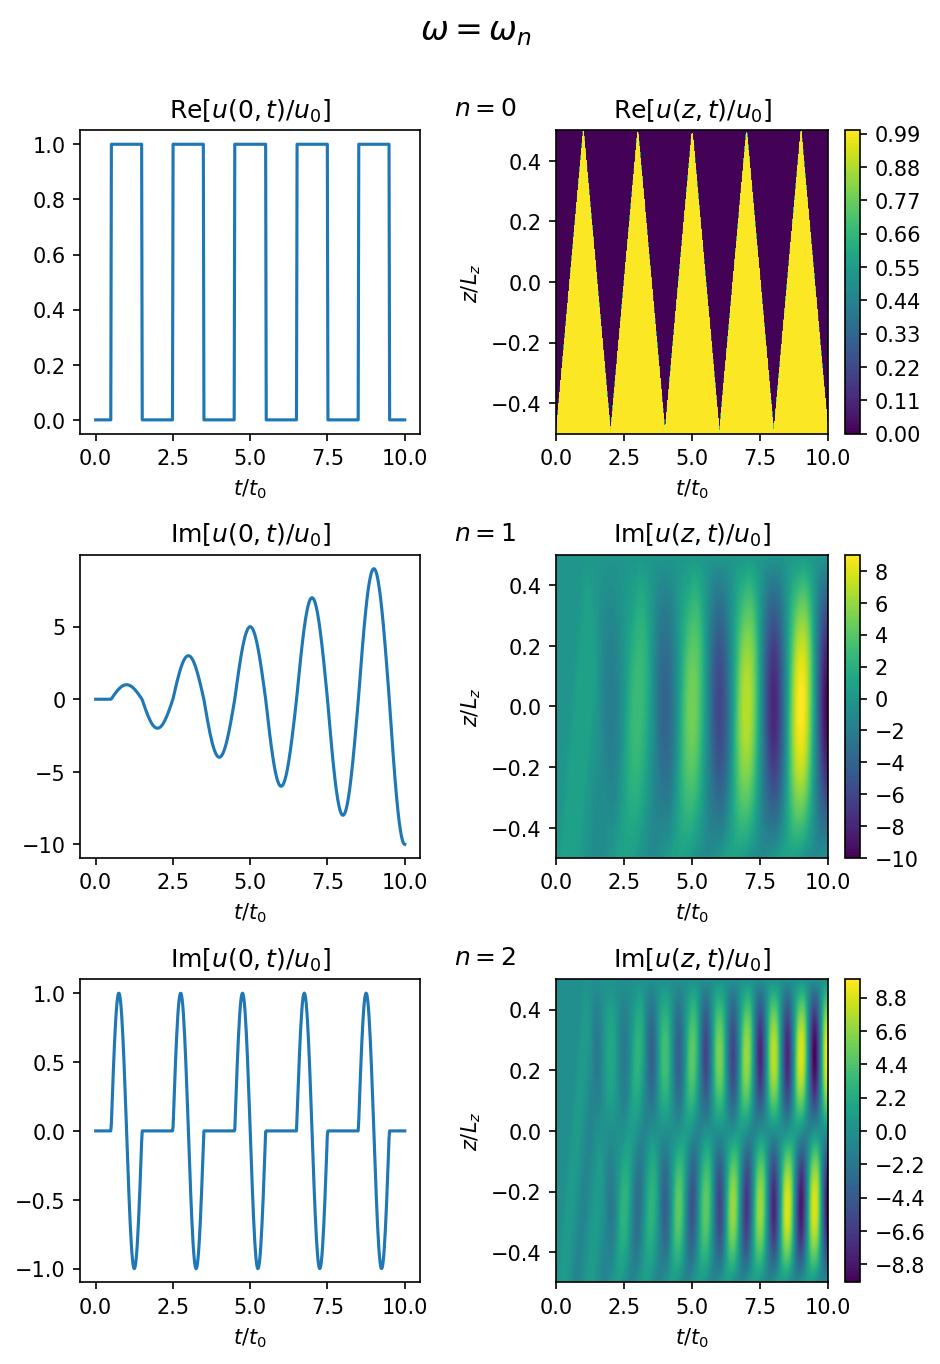
\includegraphics[width=\textwidth,height=0.85\textheight,keepaspectratio]{figures/chapter02/case_where_omega=omega_n_u.png}
    \vspace{-10pt}
    \caption{This figure shows contour plots of the velocity, $u$, and line plots at $z=0$. The driver frequency is given by $\omega=\omega_n$. Each row shows the solution for different values of $n$. The top row shows the real part and the other rows show the imaginary part. The normalising constant, $t_0$, is given by Equation \eqref{eq:t0}. The code used to make this figure is available on GitHub in the following directory:\newline
    \href{https://github.com/aleksyprok/apkp_thesis/blob/main/Python/Chapter2/case_where_omega\%3Domega_n.py}{$\rightarrow$ Python/Chapter2/case\_where\_omega=omega\_n.py}
    }
    \label{fig:case_where_omega=omega_n_u}
    \vspace{-30pt}
\end{figure}

\begin{figure}
    \centering
    \vspace{-20pt}
    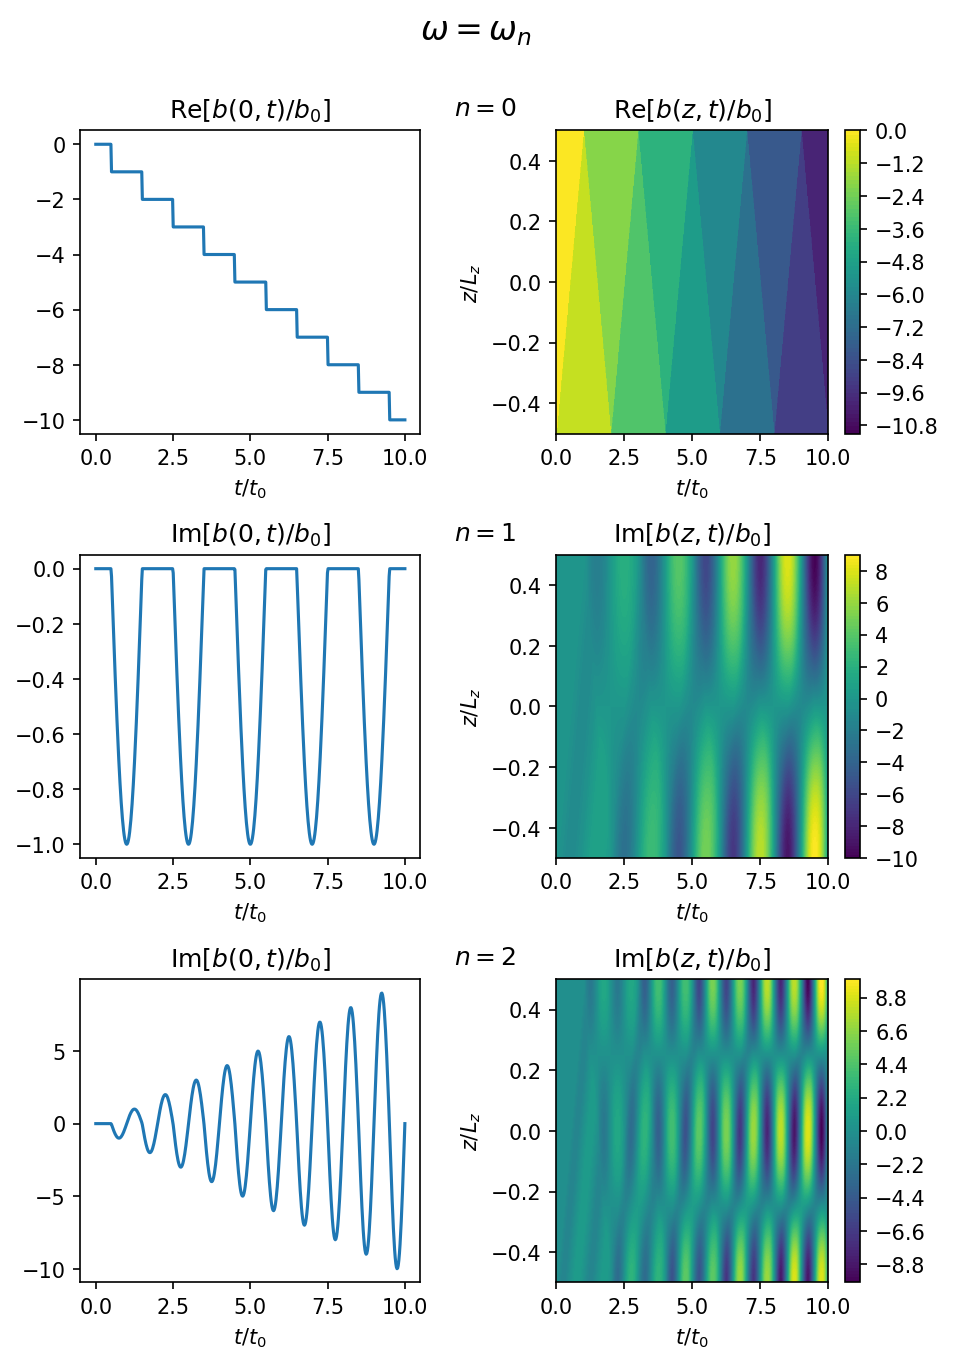
\includegraphics[width=\textwidth,height=0.9\textheight,keepaspectratio]{figures/chapter02/case_where_omega=omega_n_b.png}
    \vspace{-10pt}
    \caption{This figure is very similar to Figure \ref{fig:case_where_omega=omega_n_u} except it shows the magnetic field, $b$, instead of the velocity. The normalising constant, $b_0$, is given by Equation \eqref{eq:b0}. The code used to make this figure is available on GitHub in the following directory:\newline
     \href{https://github.com/aleksyprok/apkp_thesis/blob/main/Python/Chapter2/case_where_omega\%3Domega_n.py}{$\rightarrow$ Python/Chapter2/case\_where\_omega=omega\_n.py}}
    \vspace{-30pt}
    \label{fig:case_where_omega=omega_n_b}
\end{figure}

Figures \ref{fig:case_where_omega=omega_n_u} and \ref{fig:case_where_omega=omega_n_b} show plots of $u$ and $b$ for $\omega=0$, $\omega=\omega_1$ and $\omega_2$. The time is normalised by $t_0$ given by 
\begin{equation}
    \label{eq:t0}
    t_0=\frac{L_z}{v_{A0}}.
\end{equation}
The magnetic field is normalised by $b_0$, given by
\begin{equation}
    \label{eq:b0}
    b_0=\frac{B_0u_0}{v_{A0}.}
\end{equation}
Note that the real component is plotted for $\omega=0$ because the imaginary component gives the trivial solution. The imaginary part is plotted for $n\ge1$ because this ensures $u$ and $b$ are continuous. However, their derivatives are not continuous. In all three plots, the amplitude grows linearly with time, which means the energy grows quadratically. For $n\ge1$, driver generates standing Alfv\'en waves. The time and space averaged kinetic and magnetic energies are approximately equal. For $n=0$, the driver shears the magnetic field, and the amplitude grows linearly with time, whereas the kinetic energy oscillates about a finite value. It is convenient to categorise oscillatory motions into fast and slow motions: Slow motions are where the frequency, $f$, is smaller than $v_{A0}/L_z$, where $L_z$ gives the length of the loop. Fast motions are where the frequency is greater than $v_{A0}/L_z$. A key difference between fast and slow motions is that slow motions can generate a large build-up in magnetic energy with relatively little kinetic energy. For fast motions, the build-up in magnetic energy is approximately equal to the build-up in kinetic energy. The plots show if $u$ has an antinode at a given point in space, then $b$ has a node and vice versa.

\subsection{Approximately resonant case}
\subsubsectionmark{Approximately resonant}
\label{sec:case_where_omega_approx_omega_n}

In this section, we investigate the solutions for the case where $\omega = \omega_n + \epsilon \omega_1$, where $\epsilon\ll1$, i.e. we look at the solution where the driving frequency is nearly equal to one of the resonant frequencies.

\begin{figure}
    \centering
    \vspace{-20pt}
    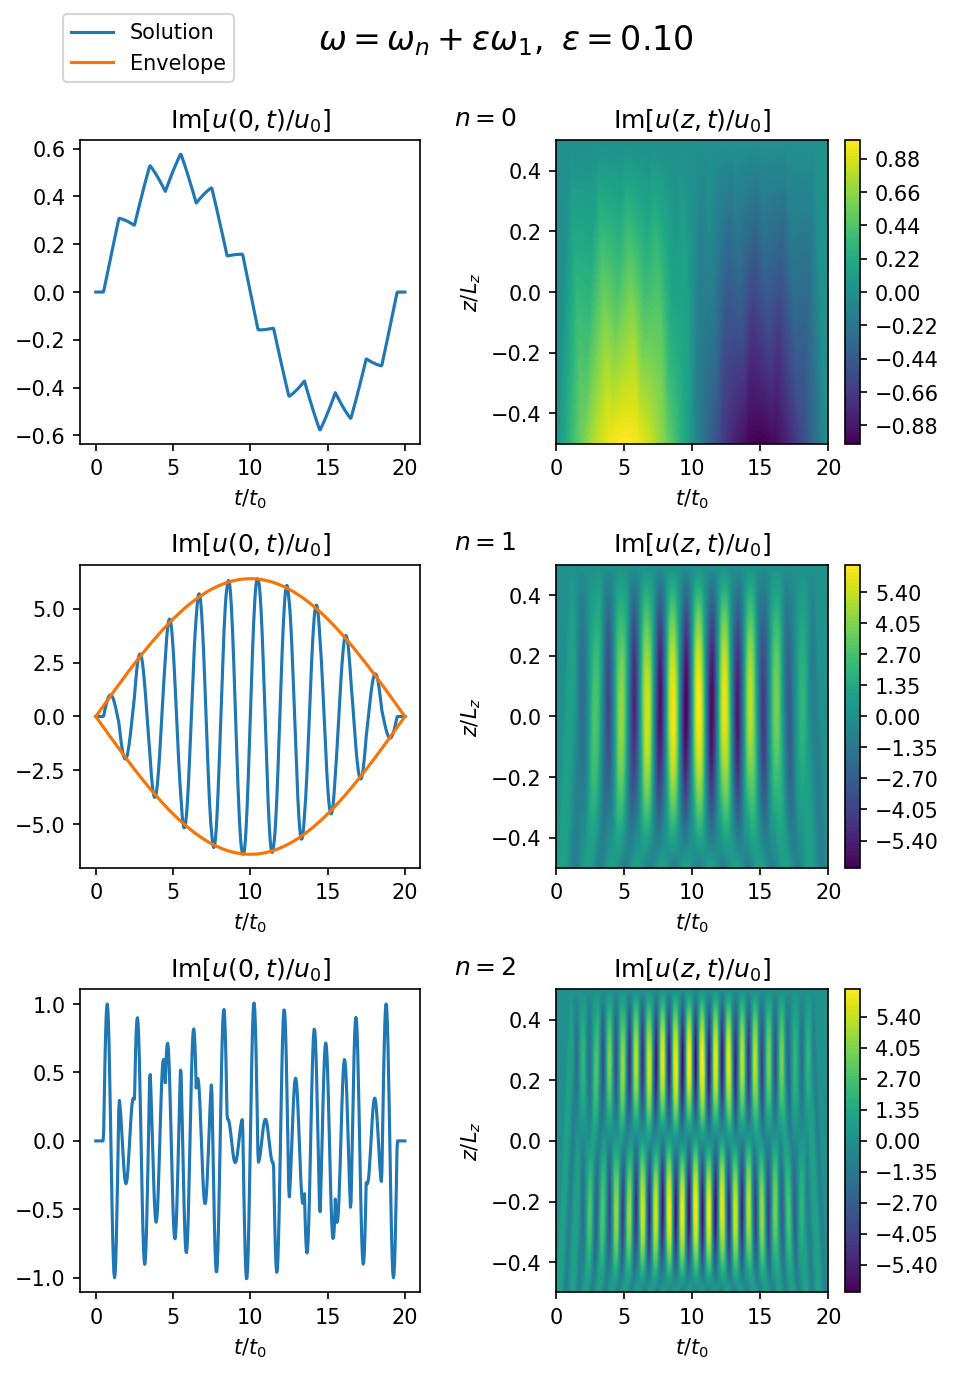
\includegraphics[width=\textwidth,height=0.85\textheight,keepaspectratio]{figures/chapter02/case_where_omega_approx_omega_n_u.png}
    \vspace{-10pt}
    \caption{This figure is similar to Figure \ref{fig:case_where_omega=omega_n_u} except now the frequency is given by $\omega=\omega_n+\epsilon \omega_1$ for $\epsilon=0.1$. Also, the imaginary component is taken for all values of $n$. Note that the velocity at $z=0$ is plotted in blue and the envelope, given by Equation \eqref{eq:u0_envelope}, is plotted in orange. The code used to make this figure is available on GitHub in the following directory:\newline
    \href{https://github.com/aleksyprok/apkp_thesis/blob/main/Python/Chapter2/case_where_omega_approx_omega_n.py}{$\rightarrow$ Python/Chapter2/case\_where\_omega\_approx\_omega\_n.py}}
    \label{fig:case_where_omega_approx_omega_n_u}
    \vspace{-30pt}
\end{figure}

\begin{figure}
    \centering
    \vspace{-20pt}
    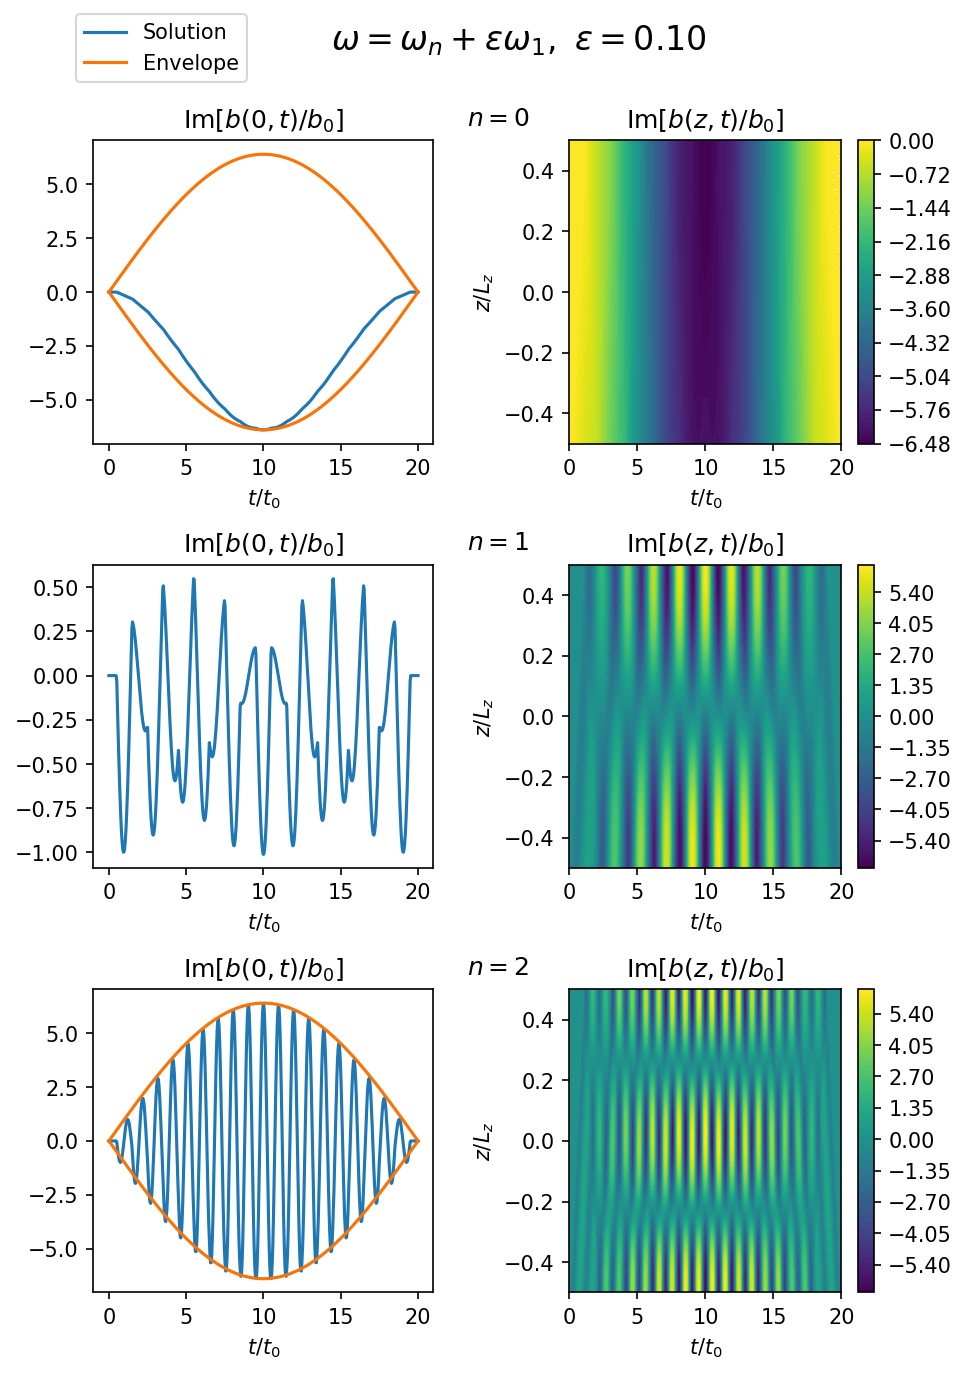
\includegraphics[width=\textwidth,height=0.9\textheight,keepaspectratio]{figures/chapter02/case_where_omega_approx_omega_n_b.png}
    \vspace{-10pt}
    \caption{This figure is similar to Figure \ref{fig:case_where_omega_approx_omega_n_u} except the magnetic field is plotted instead of the velocity. The equation for the envelope is given by Equation \eqref{eq:b0_envelope}. The code used to make this figure is available on GitHub in the following directory:\newline
    \href{https://github.com/aleksyprok/apkp_thesis/blob/main/Python/Chapter2/case_where_omega_approx_omega_n.py}{$\rightarrow$ Python/Chapter2/case\_where\_omega\_approx\_omega\_n.py}}
    \vspace{-30pt}
    \label{fig:case_where_omega_approx_omega_n_b}
\end{figure}

From Equation \eqref{eq:abs_u0_non_res} we know that the absolute value of the velocity at $z=0$ is given by
\[
    |u(0,t)|=u_0\abs{\sec(\frac{\omega l_z}{v_{A0}})\sin\qty{(m'+1)\qty(\frac{l_z}{v_{A0}}(\omega-\omega_n)+\frac{l_z \omega_n}{v_{A0}}+\frac{\pi}{2})}}.
\]
Since $m'+1\in\mathds{Z}$, then for $n$ odd we know that
\[\abs{\sin\qty{(m'+1)\qty(x + \frac{\omega_n l_z}{v_{A0}}+\frac{\pi}{2})}}=\abs{\sin\{(m'+1)x\}}.\]
Therefore, approximating $m'+1$ with 
\[m'+1\approx \frac{v_{A0} t}{L_z},\]
we can derive an equation for an envelope, $u_{e0}(t)$, that that the real and imaginary components of the velocity at $z=0$ approximately lies inside
\begin{equation}
    \label{eq:u0_envelope}
    u_{e0}(t) = \pm u_0\sec\qty(\frac{\omega l_z}{v_{A0}})\sin\qty{\frac{\omega - \omega_n}{2}t},
\end{equation}
for $n$ odd.
Using Equation \eqref{eq:abs_b0_non_res} we can derive a similar envelope, $b_{e0}(t)$ for the magnetic field at $z=0$, given by
\begin{equation}
    \label{eq:b0_envelope}
    b_{e0}(t)=\pm \frac{u_0B_0}{v_{A0}}\csc\qty(\frac{\omega l_z}{v_{A0}})\sin\qty{\frac{\omega - \omega_n}{2}t},
\end{equation}
for $n$ even.

Figures \ref{fig:case_where_omega_approx_omega_n_u} and \ref{fig:case_where_omega_approx_omega_n_b} plot the solutions for the case where $\omega=\omega_n+\epsilon \omega_1$. In all the plots the imaginary part is shown instead of the real part because it is continuous. The plots display an interference pattern called a beat. The beating angular frequency, $\omega_b$, is given by
\begin{equation}
    \omega_b = \frac{\omega - \omega_n}{2}.
\end{equation}
The beat is a concept from acoustics. It is an interference pattern between two sounds of slightly different frequencies, perceived as a periodic variation in magnitude with a rate which is the difference of the two frequencies.

\subsection{Nonresonant case}
\label{sec:case_where_omega_ne_omega_n}

In this section we consider the least resonant case, i.e. the case where
\[\omega = \frac{\omega_{n}+\omega_{n+1}}{2}.\]
This represents the least resonant case because the frequency is as far away from any of the resonant frequencies as possible. The solutions are plotted in Figure \ref{fig:case_where_omega_ne_omega_n_u} and \ref{fig:case_where_omega_ne_omega_n_b}. As expected, maximum energy of the solution is significantly smaller than the maximum energies reached in Figures \ref{fig:case_where_omega=omega_n_u}-\ref{fig:case_where_omega_approx_omega_n_b}. This is because the driver frequency is far away from the resonant and so constructive interference is quickly followed up by destructive interference which prevents the build-up of energy. For $n=3$ and $n=6$ the waves oscillate at a fixed amplitude, then after a time interval of length, $L_z / v_{A0}$, the waves oscillate at a different amplitude.

\begin{figure}
    \centering
    \vspace{-20pt}
    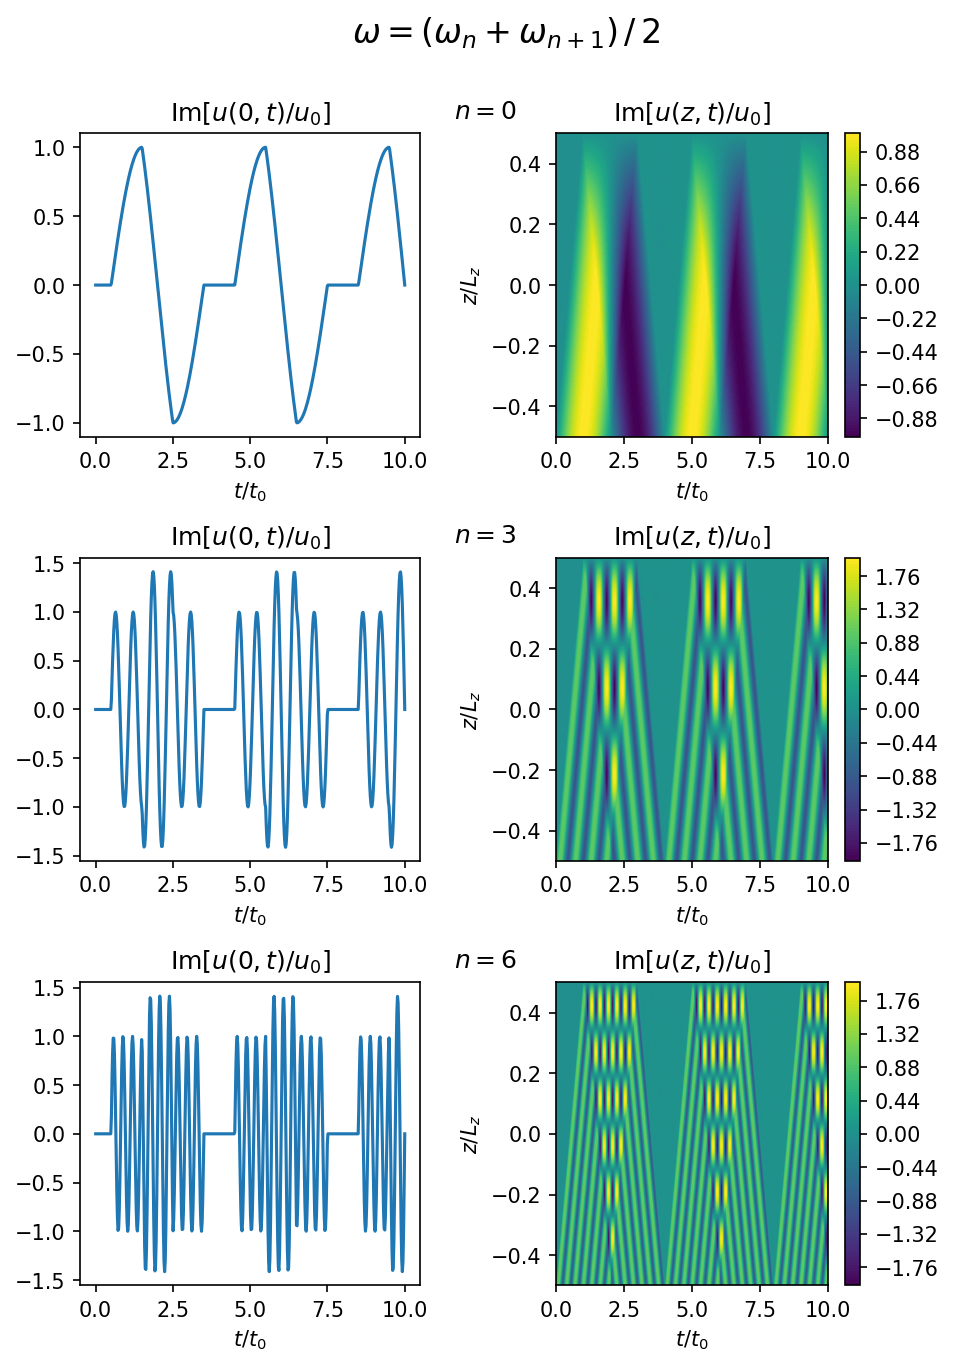
\includegraphics[width=\textwidth,height=0.9\textheight,keepaspectratio]{figures/chapter02/case_where_omega_ne_omega_n_u.png}
    \vspace{-10pt}
    \caption{This figure is similar to Figure \ref{fig:case_where_omega=omega_n_u} except now the frequency is given by $\omega=(\omega_n+\omega_{n+1})/2$. These are the least resonant frequencies because they are as far away from any of the resonant frequencies as possible. The code used to make this figure is available on GitHub in the following directory:\newline
    \href{https://github.com/aleksyprok/apkp_thesis/blob/main/Python/Chapter2/case_where_omega_ne_omega_n.py}{$\rightarrow$ Python/Chapter2/case\_where\_omega\_ne\_omega\_n.py}}
    \vspace{-30pt}
    \label{fig:case_where_omega_ne_omega_n_u}
\end{figure}

\begin{figure}
    \centering
    \vspace{-20pt}
    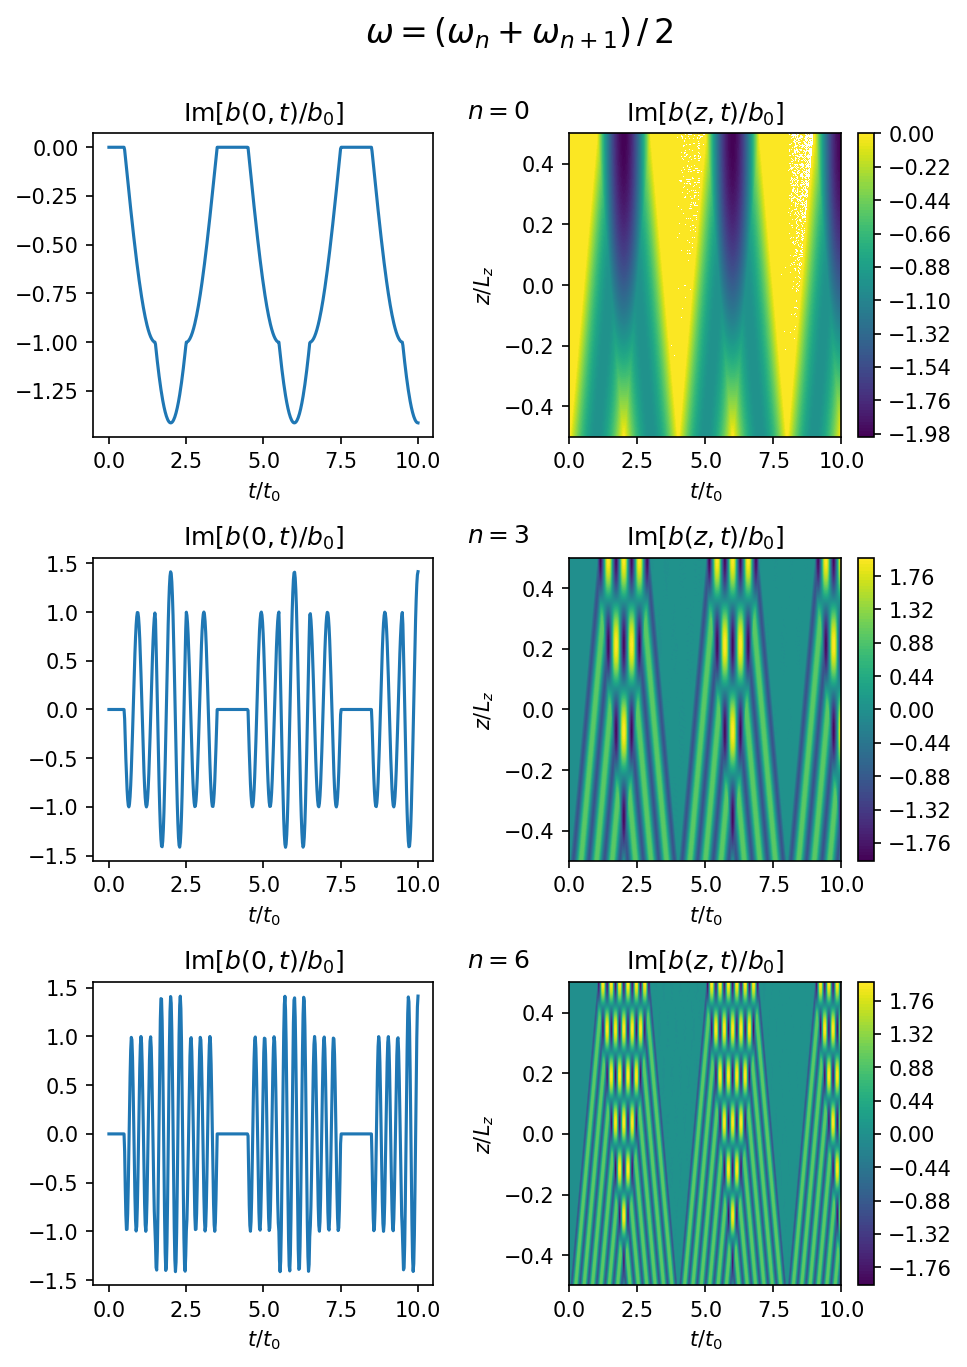
\includegraphics[width=\textwidth,height=0.9\textheight,keepaspectratio]{figures/chapter02/case_where_omega_ne_omega_n_b.png}
    \vspace{-10pt}
    \caption{This figure is similar to Figure \ref{fig:case_where_omega=omega_n_u} except the magnetic field is plotted instead of the velocity. The code used to make this figure is available on GitHub in the following directory:\newline
    \href{https://github.com/aleksyprok/apkp_thesis/blob/main/Python/Chapter2/case_where_omega_ne_omega_n.py}{$\rightarrow$ Python/Chapter2/case\_where\_omega\_ne\_omega\_n.py}}
    \vspace{-30pt}
    \label{fig:case_where_omega_ne_omega_n_b}
\end{figure}

\section{Closed loop: broadband driver}
\label{sec:closed_loop_random_driver}

This section takes a statistical approach to study the solutions for a broadband driver, i.e. a driver which excites a wide range of frequencies. The previous section calculated the solution for a single frequency driver. Figure \ref{fig:power_spectrum_morton} shows that velocity fluctuations in the corona oscillate at a wide range of frequencies. We think of the previous section as the case where the driver includes only one term in its Fourier series. In contrast, this section contains many terms, even an infinite number of terms. We can constrain the terms' amplitude using observed power spectra, e.g. Figure \ref{fig:power_spectrum_morton}. However, each term's phase cannot be constrained. Therefore, we need to consider all possible phases associated with each term in the Fourier series. Given the infinite number of possibilities, we take a statistical approach to study the solutions. We aim to study the average behaviour and answer the question: do the solutions grow to infinity or oscillate about a finite value? In the previous section, we calculated that for a sinusoidal driver, the solution's energy either oscillates about a finite value if $\omega\ne\omega_n$ or grows to infinity if $\omega=\omega_n$. To answer this question for the broadband driver, we first reduce Equation \eqref{eq:alfven_wave_equation2} to a system of ODEs, corresponding to the equation of a driven harmonic oscillator. After that, we calculate the general solution to the ODE, and then we study the case where the driver gives a red noise and white noise force.

\subsection{Driven harmonic oscillator}
\label{sec:chap_2_driven_harmonic_oscillator}

We define our $z$-range to be given by $0\le z\le L_z$ with the boundary conditions given by
\begin{equation}
    u(0,t) = f_{driv}(t),\quad u(L_z,t) = 0.
\end{equation}
Let
\begin{equation}
    u(z,t) = y(z,t) + \frac{L_z - z}{L_z}f_{driv}(t).
\end{equation}
Substituting this into Equation \eqref{eq:alfven_wave_equation2} gives
\begin{equation}
    \begin{aligned}
    \pdv[2]{y}{t}-v_{A0}^2\pdv[2]{y}{z}&=-\frac{L_z - z}{L_z}\dv[2]{f_{driv}}{t} \\
    \end{aligned}
\end{equation}
Hence, the boundary conditions for $y(z,t)$ are
\begin{equation}
    y(\pm l_z, t) = 0.
\end{equation}
We can equate the right-hand side with the following Fourier series
\begin{equation}
    -\frac{L_z - z}{L_z}f_{driv}''(t) = -2f_{driv}''(t)\sum_{n=1}^\infty \frac{\sin(k_{zn} z)}{n\pi},
\end{equation}
for $0<z\le L_z$, where
\begin{equation}
    k_{zn} = \frac{n\pi}{L_z}.
\end{equation}
Let
\begin{equation}
    y(z,t) = \sum_{n=1}^\infty y_n(t)\sin(k_{zn}z),
\end{equation}
therefore, each $y_n$ satisfies
\begin{equation}
    \label{eq:driven_harmonic_oscillator}
    \dv[2]{y_n}{t} + \omega_n^2y_n=f_n(t),
\end{equation}
where 
\begin{gather}
    \omega_n = \frac{n\pi}{L_z}v_{A0},
    f_n(t) = -2\frac{f_{driv}''(t)}{n\pi}.
\end{gather}
Note that Equation \eqref{eq:driven_harmonic_oscillator} is the equation for a driven harmonic oscillator.

\subsection{General solution}

In this section we calculate the general solution to Equation \eqref{eq:driven_harmonic_oscillator}. We first calculate a general solution using a Green's function. After that, we calculate the mean and variance of the solution for a driver with a Fourier series where each coefficient is a random number from a Gaussian probability distribution.

The Green's function, $G(t)$ for Equation \eqref{eq:driven_harmonic_oscillator} is
\begin{equation}
    G(t) = H(t)\frac{\sin(\omega_n t)}{\omega_n},
\end{equation}
where $H(t)$ is the Heaviside step function.
We impose the initial condition
\begin{equation}
    \label{eq:initial_conditions_greens_function}
    y_n(0)=\left.\dv{y_n}{t}\right|_{t=0}=0,
\end{equation}
therefore, the complementary component of the solution is zero. Hence, the general solution is given by
\begin{equation}
    \label{eq:general_soln_greens_function}
    y_n=\frac{1}{\omega_n}\int_0^t\sin[\omega_n(t-t')]f_n(t')dt'.
\end{equation}

Equation \eqref{eq:general_soln_greens_function} works for any smooth function. Now we will consider the solution where we know the Fourier series of the driver up to a statistical average. Let the following Fourier series describe $f_n(t)$,
\begin{equation}
    \label{eq:random_fourier_series}
    f_n(t)=a_0X_0 + \sum_{k=1}^\infty a_k X_k\cos(\omega_kt) + b_k Y_k \sin(\omega_k t),
\end{equation}
for $t\in[0,P]$, where
\begin{equation}
    \label{eq:omega_k}
    \omega_k = \frac{k \pi}{2P},
\end{equation}
$X_k$, $Y_k$ are independent random Gaussian variables with mean, 
\[\langle X_k \rangle = \langle Y_k \rangle = 0,\]
and variance
\[\langle X_k^2 \rangle = \langle Y_k^2 \rangle = 1.\]
Therefore, by Parseval's theorem,
\begin{equation}
    \frac{1}{2P}\int_0^{2P}f_n^2(t)dt = a_0^2X_0^2+\frac{1}{2}\sum_{k=1}^\infty a_k^2X_k^2 + b_k^2Y_k^2.
\end{equation}
Hence,
\begin{equation}
\begin{aligned}
   \left\langle\frac{1}{2P}\int_0^{2P}f_n^2(t)dt\right\rangle &= \langle a_0^2X_0^2 \rangle +\frac{1}{2}\sum_{k=1}^\infty \langle a_k^2X_k^2 \rangle + \langle b_k^2Y_k^2 \rangle \\
    &= a_0^2+\frac{1}{2}\sum_{k=1}^\infty a_k^2 + b_k^2.
\end{aligned}
\end{equation}
Therefore, the coefficients $a_k$, $b_k$ give the average power spectrum of $f_n(t)$. We can use data from observations, e.g. Figure \ref{fig:power_spectrum_morton} to determine the values of $a_k$, $b_k$.

Using Equation \eqref{eq:general_soln_greens_function}, the solution for $f_n(t)$ given by Equation \eqref{eq:random_fourier_series} is
\begin{equation}
    \label{eq:velocity_soln_random_fourier_driver}
    y_n(t) = \sum_{k=0}^\infty y_n^{(k)}(t),
\end{equation}
where
\begin{equation}
    y_n^{(k)}(t) = \frac{a_k X_k\omega_n\qty[\cos(\omega_n t) - \cos(\omega_k t)] + b_k Y_k\qty[\omega_k\sin(\omega_n t) - \omega_n\sin(\omega_k t)]}{\omega_n(\omega_k^2 - \omega_n^2)},
\end{equation}
for $\omega_k\ne \omega_n$ and
\begin{equation}
    y_n^{(k)}(t) = \frac{a_k X_k\omega_n t \sin(\omega_n t) + b_k Y_k\qty[\sin(\omega_n t) - \omega_n t \cos(\omega_n t)]}{2\omega_n^2},
\end{equation}
for $\omega_k = \omega_n$. Therefore, the mean $\langle y_n(t) \rangle = 0$ and the variance is given by
\begin{equation}
    \label{eq:variance_fourier}
    \langle y_n^2(t) \rangle = \sum_{k=0}^\infty \left\langle \qty[y_n^{(k)}(t)]^2 \right\rangle,
\end{equation}
where
\begin{equation}
    \label{eq:variance_omega_ne_omega_k}
    \left\langle \qty[y_n^{(k)}(t)]^2 \right\rangle = \frac{a_k^2 \omega_n^2\qty[\cos(\omega_n t) - \cos(\omega_k t)]^2 + b_k^2 \qty[\omega_k\sin(\omega_n t) - \omega_n\sin(\omega_k t)]^2}{\omega_n^2(\omega_k^2 - \omega_n^2)^2},
\end{equation}
for $\omega_k\ne\omega_n$ and
\begin{equation}
    \label{eq:variance_omege=omega_k}
    \left\langle \qty[y_n^{(k)}(t)]^2 \right\rangle = \frac{a_k^2 \omega_n^2 t^2 \sin^2(\omega_n t) + b_k^2 \qty[\sin(\omega_n t) - \omega_n t \cos(\omega_n t)]^2}{4\omega_n^4},
\end{equation}
if $\omega_k=\omega_n$. This shows that in general, the power spectrum will have a peak at the resonant frequencies.

Here we calculate the time-derivative of the variance because we will need it in Section \ref{sec:noisy_force}. The time-derivative of $y_n(t)$ is given by
\begin{equation}
    \dv{y_n}{t} = \sum_{k=0}^\infty\dv{y_n^{(k)}}{t},
\end{equation}
where
\begin{equation}
    \dv{y_n^{(k)}}{t} = \frac{a_k X_k\qty[\omega_k\sin(\omega_k t) - \omega_n\sin(\omega_n t) ] + b_k Y_k \omega_k\qty[\cos(\omega_n t) - \cos(\omega_k t)]}{\omega_k^2 - \omega_n^2},
\end{equation}
for $\omega_k\ne \omega_n$ and
\begin{equation}
    \label{eq:variance_d_velocity_dt}
    \dv{y_n^{(k)}}{t} = \frac{a_k X_k [\sin(\omega_n t) + \omega_n t \cos(\omega_n t)]+ b_k Y_k \omega_n t \sin(\omega_n t)}{2\omega_n},
\end{equation}
for $\omega_k = \omega_n$. Therefore, the mean $\langle \dv*{y_n}{t} \rangle = 0$ and the variance is given by
\begin{equation}
    \left\langle \qty[\dv{y_n}{t}]^2 \right\rangle = \sum_{k=0}^\infty \left\langle \qty[\dv{y_n^{(k)}}{t}]^2 \right\rangle,
\end{equation}
where
\begin{equation}
    \left\langle \qty[\dv{y_n^{(k)}}{t}]^2 \right\rangle = \frac{a_k^2\qty[\omega_k\sin(\omega_k t) - \omega_n\sin(\omega_n t)]^2 + b_k^2\omega_k^2 \qty[\cos(\omega_n t) - \cos(\omega_k t)]^2}{(\omega_k^2 - \omega_n^2)^2},
\end{equation}
for $\omega_k\ne\omega_n$ and
\begin{equation}
   \left\langle \qty[\dv{y_n^{(k)}}{t}]^2 \right\rangle = \frac{a_k^2 [\sin(\omega_n t) + \omega_n t \cos(\omega_n t)]^2+ b_k^2  \omega_n^2 t^2 \sin^2(\omega_n t)}{4\omega_n^2},
\end{equation}
if $\omega_k=\omega_n$.

\subsection{Noisy force}
\label{sec:noisy_force}

Let $\eta(t)$ be a noisy signal, given by
\begin{equation}
    \eta(t) = \int_{-\infty}^\infty \hat{\eta}(f)\exp(2\pi i t f) df,
\end{equation}
where its Fourier transform in the sense of distributions, $\hat{\eta}(f)$, is given by
\begin{equation}
    \begin{aligned}
    \hat{\eta}(f) &= \int_{-\infty}^\infty \eta(t)\exp(-2\pi i t f) dt, \\
    \end{aligned}
\end{equation}
where $f$ denotes the frequency. We define $\eta(t)$ to be a white noise signal of strength $D$. The value of $\eta(t)$ for any time $t$ is a random Gaussian variable that is statistically independent of its entire history before. Its power spectrum is given by
\begin{equation}
    \left\langle|\hat{\eta}(f)|^2\right\rangle = D,
\end{equation}
where $D$ is a constant.
Similarly, we define $W(t)$ to be red noise of strength $E$ if it is a random signal with a power spectrum given by
\begin{equation}
    \left\langle|\hat{W}(f)|^2\right\rangle = E f^{-2},
\end{equation}
where $E$ is a constant. Red noise is often called brown noise due to its association with Brownian motion. We think of it as the integral of white noise, and it is closely related to the Wiener process. The colour of the noise takes its name from its power spectrum. White noise excites all frequencies equally and is analogous to visible white light which contains all frequencies in the rainbow. Red noise has more energy in the lower frequencies, similar to visible red light and is at the lower end of the visible light frequency spectrum.

Let the displacement, $x_n$, be given by
\begin{equation}
    \dv{x_n}{t} = y_n.
\end{equation}
Let the acceleration, $g_n$, be given by
\begin{equation}
    \dv{g_n}{t} = f_n.
\end{equation}
Substituting the above two equations into Equation \eqref{eq:driven_harmonic_oscillator} and integrating gives
\begin{equation}
    \label{eq:driven_harmonic_oscillator_displacement}
    \dv[2]{x_n}{t} + \omega_n^2x_n=g_n(t) + C,
\end{equation}
where $C$ is an integration constant. We consider the case where the integration constant $C$ equals 0 as the solution associated with this term can be superimposed if needed. Equation \eqref{eq:driven_harmonic_oscillator_displacement} shows that $g_n(t)$ has the dimensions of a force (divided by mass). Therefore, if $g_n(t)=\eta(t)$ we say the system is driven by a white noise force and if $g_n(t)=W(t)$ then the system is driven by a red noise force. We are interested in red and white noise because they power produce spectra with slopes $f^0$ and $f^{-2}$. Fitting Figure \ref{fig:power_spectrum_morton} with a single power law shows the velocity fluctuations in the solar corona have a power spectrum which goes as $f^p$, where $-2<p<0$. If $g_n(t)=\eta(t)$, then we solve Equation \eqref{eq:driven_harmonic_oscillator_displacement}. If $g_n(t)=W(t)$, then $f_n(t)=\eta(t)$ and so we solve Equation \eqref{eq:driven_harmonic_oscillator}. In other words, we solve the equation where white noise is on the right hand side. In this section we will solve for the case where $g_n(t)=W(t)$, then we use a trick where we substitute $\dv*{y_n}{t}\rightarrow y_n$ to quickly calculate the solution for the case where $g_n = \eta(t)$. Note that this substitution causes the initial conditions, see Equation \eqref{eq:initial_conditions_greens_function}, to change to 
\begin{equation}
    x_n(0) = \dv{x_n}{t} = 0.
\end{equation}

By the Wiener–Khinchin theorem, $\eta(t)$ has an autocorrelation given by the Fourier transform of the power spectral density, i.e.
\begin{equation}
    \label{eq:autocorrelation}
    \begin{aligned}
    \langle\eta(t) \eta(t')\rangle &= \int_{\infty}^\infty \left\langle\abs{\hat{\eta}(\xi)}^2\right\rangle\exp[2\pi i \xi (t - t')] d\xi \\
    &=D\delta(t-t'),
    \end{aligned}
\end{equation}
where $\delta(t-t')$ is the Dirac delta function. 
If $f_n(t)$ is a white noise signal then Equation \eqref{eq:driven_harmonic_oscillator} gives a Langevin equation where an exact solution can be calculated with a simpler solution compared with Equation \eqref{eq:driven_harmonic_oscillator}. Substituting $f_n(t)=\eta(t)$ into Equation \eqref{eq:driven_harmonic_oscillator} gives the following Langevin equation
\begin{equation}
    \dv[2]{y_n}{t} + \omega_n^2 y_n = \eta(t).
\end{equation}
Note that $\eta(t)$ has a mean of
\begin{equation}
    \langle\eta(t)\rangle=0.
\end{equation}
Using Equation \eqref{eq:general_soln_greens_function}, the solution is given by
\begin{equation}
    y_n = \frac{1}{\omega_n}\int_0^t\sin[\omega_n(t-t')]\eta(t')dt',
\end{equation}
and
\begin{equation}
    \dv{y_n}{t} = \int_0^t\cos[\omega_n(t-t')]\eta(t')dt'.
\end{equation}
Hence, the mean of $y_n$ is given by
\begin{equation}
    \begin{aligned}
    \langle y_n \rangle &= \frac{1}{\omega_n}\int_0^t\sin[\omega_n(t-t')]\langle \eta(t') \rangle dt' \\
    &= 0.
    \end{aligned}
\end{equation}
The square of $y_n$ is given by
\begin{equation}
    y_n^2 = \frac{D^2}{\omega_n^2}\int_0^t\int_0^t\sin[\omega_n(t-t')]\sin[\omega_n(t-t'')]\eta(t')\eta(t'')dt'dt''.
\end{equation}
Hence, the variance of $y_n$ is given by
\begin{equation}
    \label{eq:variance_exact_red_force}
    \begin{aligned}
    \langle y_n^2 \rangle &= \frac{1}{\omega_n^2}\int_0^t\int_0^t\sin[\omega_n(t-t')]\sin[\omega_n(t-t'')]\langle \eta(t')\eta(t'')\rangle dt'dt'' \\
    &= \frac{D}{\omega_n^2}\int_0^t\int_0^t\sin[\omega_n(t-t')]\sin[\omega_n(t-t'')]\delta(t'-t'') dt'dt'' \\
    &= \frac{D}{\omega_n^2}\int_0^t\sin^2[\omega_n(t-t')] dt' \\
    &=\frac{D}{2\omega_n^3}[\omega_n t - \sin(\omega_n t) \cos(\omega_n t)].
    \end{aligned}
\end{equation}
Similarly, the mean of $\dv*{y_n}{t}$ is 
\begin{equation}
    \left\langle \dv{y_n}{t} \right\rangle=0.
\end{equation}
The variance is given by
\begin{equation}
    \left\langle \qty[\dv{y_n}{t}]^2 \right\rangle=\frac{D}{2\omega_n}[\omega_n t + \sin(\omega_n t) \cos(\omega_n t)].
\end{equation}
This shows that for both a red/white noise driver the energy on average goes to infinity. For a single frequency resonant driver the amplitude grows linearly with time whereas for a white/red noise driver, the standard deviation grows as $\sqrt{t}$. However, white noise drivers are unphysical because they have an infinite variance. The variance of $\eta(t)$ is given by its autocorrelation for $t=t'$. Equation \eqref{eq:autocorrelation} shows that variance is infinite, and this is because white noise excites all the frequencies from $0$ to $\infty$. Equation \eqref{eq:variance_omega_ne_omega_k} shows that the variance associated with the higher frequency drivers goes to $0$ as $f\rightarrow\infty$. For this reason, we predict the solutions above provide a good approximation for solutions where the driver only excites frequencies up to a finite value, provided the resonant frequency is excited. To test this prediction, the next paragraph calculates the solution for a more physical driver which excites a finite range of frequencies causing it to have a finite variance.

Our goal is to ensure $f_n(t)$ excites each frequency with the same strength as $\eta(t)$ but only for a finite number of frequencies.
Note that Equation \eqref{eq:random_fourier_series} can be written as
\begin{equation}
    f_n(t) = \sum_{k=-\infty}^\infty C_k\exp[2\pi i f_k t] \Delta f,
\end{equation}
where
\begin{gather}
     C_k = \begin{cases}
    4Pa_0 X_0, & k=0, \\
    2P(a_kX_k - i b_k Y_k), & k>0, \\
    C^*_{\abs{k}}, k<0,
    \end{cases} \\
    f_k = \frac{k}{4P}, \\
    \Delta f = \frac{1}{4P}.
\end{gather}
For $P\rightarrow\infty$
\[f_k \rightarrow f,\]
\[\Delta f \rightarrow df,\]
\[C_k \rightarrow C(f),\]
hence,
\begin{equation}
    f_n(t) \rightarrow \int_{-\infty}^\infty C(f) \exp[2\pi i f t] df.
\end{equation}
By the Wiener–Khinchin theorem,
\begin{equation}
    \begin{aligned}
    \implies \langle f_n^2(t)\rangle &= \sum_{k=-\infty}^\infty \left\langle\abs{C_k}^2\right\rangle\exp[2\pi i f t] \\
    &\rightarrow \int_{-\infty}^\infty \left\langle\abs{C(f)}^2\right\rangle \exp[2\pi i f t] d f. \\
    \end{aligned}
\end{equation}
Hence, we require
\begin{equation}
    \left\langle\abs{C_k}^2\right\rangle = \frac{D}{\Delta f}.
\end{equation}
Note that
\begin{equation}
    \langle \abs{C_k}^2 \rangle = \begin{cases}
    (4Pa_0)^2, & k=0, \\
    4P^2(a_k^2 + b_k^2), & k\ne0,
    \end{cases}
\end{equation}
therefore, letting $a_k=b_k$ gives
\begin{equation}
\label{eq:coeffs_ak_bk}
\implies
    \begin{pmatrix}
    a_0 \\
    a_k \\
    b_k
    \end{pmatrix}
    = \frac{1}{2}\sqrt{\frac{D}{P}}
    \begin{pmatrix}
    1 \\
    \sqrt{2} \\
    \sqrt{2}
    \end{pmatrix}.
\end{equation}
Equation \eqref{eq:variance_fourier}, with the coefficients above gives an  $f_n(t)$ which excites each frequency with the same strength as $\eta(t)$ but only for a finite number of frequencies.

\begin{figure}
    \centering
    \vspace{-20pt}
    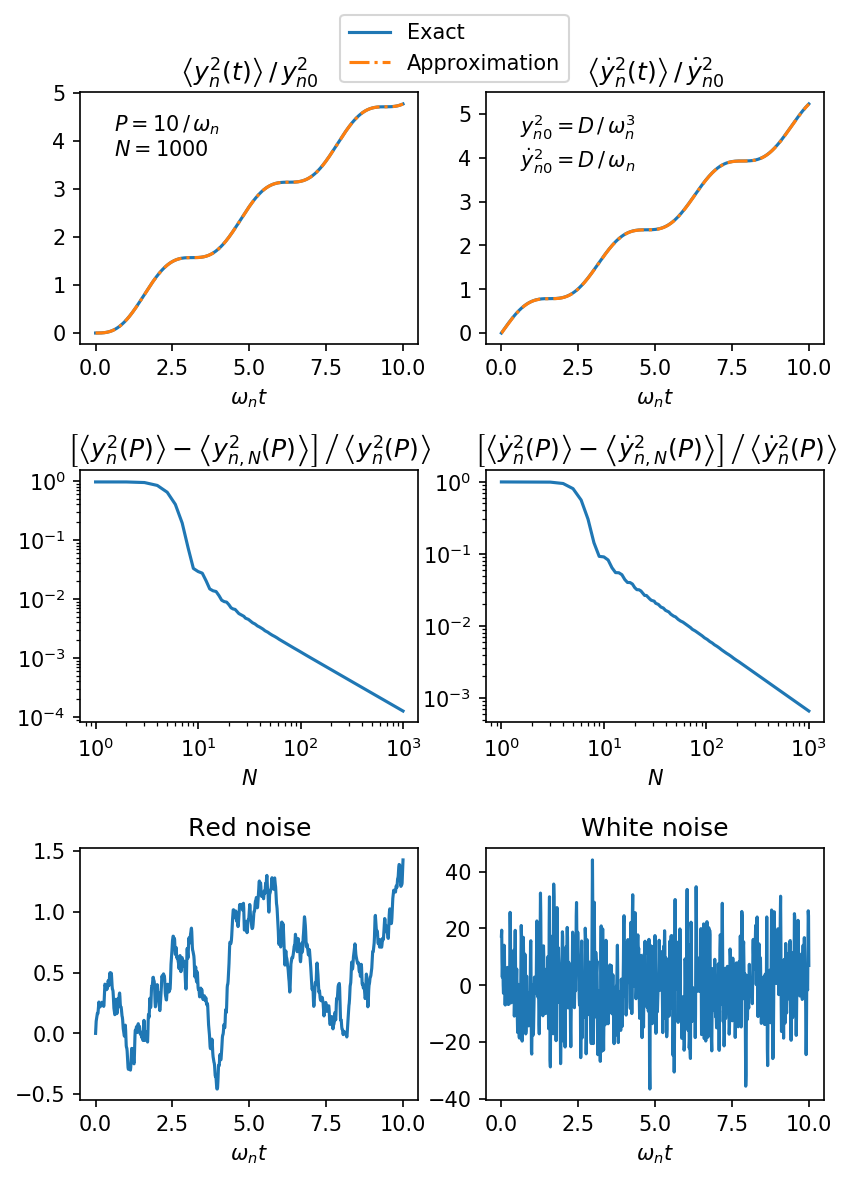
\includegraphics[width=\textwidth,height=0.8\textheight,keepaspectratio]{figures/chapter02/noisy_driver.png}
    \vspace{-10pt}
    \caption{This figure's top row shows the normalised variance of $y_n$ and $\dot{y}_n$, where we use Newton's dot notation to denote the time derivative. They plot the exact solution and the Fourier approximations. The equations for the normalising constants, $y_{n0}$ and $\dot{y}_{n0}$ is also shown. The middle row shows the error at $t=P$ between the exact solution and the Fourier approximation as a function of the number of terms in the approximation. Finally, the bottom row illustrates an example of red and white noise. The code used to make this figure is available on GitHub in the following directory:\newline
    \href{https://github.com/aleksyprok/apkp_thesis/blob/main/Python/Chapter2/random_driver.py}{$\rightarrow$ Python/Chapter2/random\_driver.py}}
    \vspace{-20pt}
    \label{fig:noisy_driver}
\end{figure}

Our goal now is to test our prediction that Equation \eqref{eq:variance_fourier} gives the same solution as Equation \eqref{eq:variance_exact_red_force} with the coefficients given by Equation \eqref{eq:coeffs_ak_bk}. We approximate the sum given by Equation \eqref{eq:variance_fourier} numerically and so the series is truncated at $k=N$. We denote that truncated approximation of Equation \eqref{eq:variance_fourier} with
\begin{equation}
    \label{eq:variance_fourier_truncated}
    \langle y_{n,N}(t) \rangle =\sum_{k=0}^N \langle y_n^{(k)} \rangle.
\end{equation}
We refer to the solution given by Equation \eqref{eq:variance_fourier_truncated} as the Fourier approximation and the solution given by Equation \eqref{eq:variance_exact_red_force} as the exact solution. The top row of Figure \ref{fig:noisy_driver} shows the variance of $y_n$ and its time derivative. It shows that for $P=10/\omega_n$ and $N=1000$ that the exact solution and Fourier approximation are in approximate agreement. The second row shows the error for the variance at $t=P$ between the exact solution and the Fourier approximation as a function of the number of terms in the truncated Fourier series. It shows that increasing the number of terms causes the error to decrease. Note that $P=10/\omega_n$, therefore, from Equation \eqref{eq:omega_k} we know that
\[\omega_k = \frac{k\pi}{20}\omega_n,\]
hence, $\omega_k>\omega_n$ for $k>6$.
The middle row of Figure \ref{fig:noisy_driver} shows that for $N\approx6$, the accuracy sharply improves for increasing $N$. This suggests that provided the resonant frequency is excited then the exact solution and Fourier approximation show approximate agreement. Therefore, the solution given by white noise which only excites frequencies over a finite range can approximate the solution given by $\eta(t)$ which excites all the frequencies from 0 to $\infty$. Finally, the bottom row of Figure \ref{fig:noisy_driver} shows an illustration of red and white noise. The white noise plot was produced using a truncated approximation of Equation \eqref{eq:random_fourier_series}, with $N=1000$. The red noise plots show the time integral of the white noise plot. The white noise plot shows an example of white noise where only a finite range of frequencies is excited. Note that it has a finite variance, whereas, $\eta(t)$, which excites all frequencies, has an infinite variance.

\section{Leaky loop: reflection coefficient}
\label{sec:leaky_loop_reflection_coefficent}

In previous sections, we modelled the boundary of the domain as a solid wall. This is a good leading order approximation for the boundary between the corona and the lower layers of the atmosphere. Figure \ref{fig:VAL_atmosphere} shows that the chromosphere and photosphere are orders of magnitude denser than the corona. We can approximate this as a solid wall, provided the wavelength of the waves is significantly longer than length-scale of the density variations. In this section, we aim to calculate an approximation for the Alfv\'en wave reflection coefficient at the corona/chromosphere interface. In other words, we aim to calculate on average how much energy is reflected and transmitted for waves at the boundary of the corona. In previous sections, we modelled perfect reflection, i.e. we assumed 100\% of the energy reflects at the boundary.  Therefore, we described the loops as closed. In this section, the reflection coefficient is less than unity so that some energy can escape. Therefore, we describe the loops as leaky.

To estimate the reflection coefficient, we use a method very similar to that described in \citet{Hollweg1984b}. We model the background Alfv\'en speed as 
\begin{equation}
    \label{eq:alfven_speed_exponential}
    v_A(z) = \begin{cases}
    v_{A0}\exp(z/(2h)), & z < 0, \\
    v_{A0}, & z\ge 0, \\
    \end{cases}
\end{equation}
where $h$ gives the pressure scale height which is defined as
\begin{equation}
    \label{eq:pressure_scale_height}
    h = \frac{k_B T}{m g_\odot},
\end{equation}
where $k_B$ is the Boltzmann constant, $T$ is the mean plasma temperature, $m$ is the mean mass of a molecule, and $g_\odot$ is the gravitational acceleration given by Equation \eqref{eq:gravitational_acceleration}. We choose the Alfv\'en speed (see Equation \ref{eq:alfven_speed_exponential}), to approximate the solar atmosphere's Alfv\'en speed profile, where $z<0$ corresponds to the photosphere and chromosphere and $z>0$ corresponds to the corona. We model the corona as uniform for convenience.

To estimate the the reflection coefficient, we calculate the general normal mode solution for $z<0$ and $z\ge0$ and apply the boundary condition that the the source of the waves lies in $z>0$. After that we calculate the coefficients which ensure continuity of $u$ and $\pdv*{u}{z}$ at $z=0$. First, we prove that $u$ and $\pdv*{u}{z}$ must be continuous at $z=0$. Write the Alfv\'en wave equation, Equation \eqref{eq:alfven_wave_equation2}, as
\[\pdv[2]{u}{z}=\frac{1}{v_A^2(z)}\pdv[2]{u}{t}.\]
Integrate from $z=-\epsilon$ to $z=\epsilon$,
\[\qty[\pdv{u}{z}]_{-\epsilon}^\epsilon=\int_{-\epsilon}^\epsilon\frac{1}{v_A^2(z)}\pdv[2]{u}{t}dz.\]
Let $\epsilon\rightarrow0$. Note that $u$ and $v_A$ are finite and so the right-hand-side must go to zero as $\epsilon\rightarrow 0$. Therefore,
\[\left.\pdv{u}{z}\right|_{\epsilon}=\left.\pdv{u}{z}\right|_{-\epsilon},\quad \epsilon\rightarrow0,\]
which implies $u$ and $\pdv*{u}{z}$ must be continuous.

We calculate normal mode solutions, i.e. we assume a time-dependence of the form $\exp(i\omega t)$. Hence, Equation \eqref{eq:alfven_wave_equation2} can be written as
\begin{equation}
    \label{eq:alfven_wave_normal_mode_eqn}
    \dv[2]{u}{z}+\frac{\omega^2}{v_A^2(z)}u=0,
\end{equation}
where to keep the notation tidy we assume the time-dependence implicitly.

Here we calculate the normal mode solution for $z<0$. Let 
\begin{equation}
    \xi(z)=\frac{2h\omega}{v_A(z)}.
\end{equation}
Note that
\[\dv{\xi}{z}=-\frac{\xi}{2h},\]
\[\dv[2]{\xi}{z}=\frac{\xi}{4h^2}.\]
Hence,
\[\dv{}{z}=\dv{\xi}{z}\dv{}{\xi}\]
\[\begin{aligned}
\dv[2]{}{z}&=\qty(\dv{\xi}{z})^2\dv[2]{}{\xi}+\dv{\xi}{z}\dv{}{\xi}\qty(\dv{\xi}{z})\dv{}{\xi} \\
&=\frac{\xi^2}{4h^2}\dv[2]{}{\xi}+\frac{\xi}{4h^2}\dv{}{\xi}.
\end{aligned}\]
Therefore, multiplying Equation \eqref{eq:alfven_wave_normal_mode_eqn} through by $4h^2$ gives
\begin{equation}
    \xi^2\dv[2]{u}{\xi}+\xi\dv{u}{\xi}+\xi^2u=0.
\end{equation}
This is the zeroth order Bessel's equation which has the general solution
\begin{equation}
    \label{eq:general_soln_z_lt_0}
    u(\xi)= C_1J_0(\xi) + C_2Y_0(\xi),\quad z<0,
\end{equation}
where $J_0(x)$ is the Bessel function of the first kind of order 0 and $Y_\alpha(x)$ is the Bessel function of the second kind of order 0. 

To apply boundary conditions to Equation \eqref{eq:general_soln_z_lt_0} we need to know which component of the solution corresponds to outward going waves (away from the corona) and inward going waves (towards the corona). To work this out, we need to calculate the Poynting flux. Using Equation \eqref{eq:by_eqn_linear} we know that $b(\xi)$ is given by
\begin{equation}
    \begin{aligned}
    b(\xi) &= \frac{B_0}{i\omega}\dv{u}{z} \\
    &= \frac{iB_0\xi}{2h\omega}\dv{}{\xi}\qty[C_1J_0(\xi) + C_2Y_0(\xi)],\quad z<0.
    \end{aligned}
\end{equation}
Using Equation \eqref{eq:poynting_flux_linear}, we know that the Poynting flux in the $z$-direction, $S_z=\vec{S}\cdot\vec{\hat{z}}$ is given by
\begin{equation}
    \label{eq:poynting_flux_chap_2}
    \begin{aligned}
    S_z&=-\frac{B_0}{\mu}\Re(u)\Re(b) \\
    &=-\frac{B_0}{\mu}\qty(\frac{u+\bar{u}}{2})\qty(\frac{b+\bar{b}}{2}),
    \end{aligned}
\end{equation}
where $\bar{u}$ denotes the complex conjugate of $u$.
Therefore, the component which does not time-average to zero is
\[
    \begin{aligned}
    \langle S_z\rangle &= -\frac{B_0}{4\mu}(u\bar{b} + \bar{u}b) \\
    &=-\frac{iB_0^2\xi}{8\mu h\omega}[(\bar{C}_1J_0+\bar{C}_2Y_0)(C_1J_0'+C_2Y_0')-(C_1J_0+C_2Y_0)(\bar{C}_1J_0'+\bar{C}_2Y_0')]\\
    &=-\frac{iB_0^2\xi}{8\mu h\omega}(\bar{C}_1C_2-C_1\bar{C}_2)(J_0Y_0'-J_0'Y_0).\\
    \end{aligned}
\]
Note that the Wronskian, $W(J_0,Y_0)(\xi)$, is given by
\begin{equation}
    \label{eq:wronskian_j0_y0}
    W(J_0,Y_0)(\xi) = J_0Y_0'-J_0'Y_0 = \frac{2}{\pi \xi}.
\end{equation}
Let
\begin{equation}
    \begin{aligned}
        C_1 &= c_1 + c_2, \\
        C_2 &= i(c_1 - c_2),
    \end{aligned}
\end{equation}
therefore,
\[\bar{C}_1C_2-C_1\bar{C}_2=2i(|c_1|^2-|c_2|^2)\]
Hence, the time-averaged Poynting flux is given by
\begin{equation}
    \label{eq:avg_poynting_flux_chap_2}
    \langle S_z\rangle=\frac{B_0^2}{8\pi\mu h\omega}\qty(|c_1|^2-|c_2|^2),
\end{equation}
where
\begin{equation}
    u(\xi) = c_1H_0^{(1)}(z) + c_2H_0^{(2)}(z),
\end{equation}
where $H_0^{(1)}$, $H_0^{(2)}$ are zeroth-order Hankel functions of the first and second kind. From the form of Equation \eqref{eq:avg_poynting_flux_chap_2}, we identify the $H_0^{{(1)}}$ and $H_0^{(2)}$ parts of the equations as the inward (towards the corona) and outward (away from the corona) propagating waves respectively. Therefore, applying boundary conditions, we set $c_1=0$ as we assume the source of the waves lies inside the corona.

Hence, the full solution for $u(z)$ is given by
\begin{equation}
    \label{eq:reflection_coefficent_u}
    u(z) = \begin{cases}
    c_2 H_0^{(2)}(\xi), & \text{for}\ z<0,\\
    c_3\exp(ik_z z) + c_4\exp(-ik_z z), & \text{for}\ z\ge0,
    \end{cases}
\end{equation}
where $k_z$ is given by
\begin{equation}
    k_z = \frac{\omega}{v_{A0}}.
\end{equation}
Using the identity
\begin{equation}
    \dv{J_0}{\xi}=-J_0(\xi),\ \dv{Y_0}{\xi}=-Y_0(\xi)\implies \dv{H_0^{(2)}}{\xi}=-H_1^{(2)}(\xi),
\end{equation}
we can show that
\begin{equation}
    \label{eq:reflection_coefficent_du_dz}
    \dv{u}{z}=\begin{cases}
    c_2(\omega / v_A)H_1^{(2)}(\xi), & \text{for}\ z<0, \\
    ic_3k_z\exp(ik_z z) - ic_4k_z\exp(-ik_z z), & \text{for}\ z\ge0. \\
    \end{cases}
\end{equation}
Note that $c_3$ gives the amplitude of the coronal incident wave which we arbitrarily choose to have an amplitude $u_0$. We require continuity of $u$ and $\dv*{u}{z}$, this gives 2 equations and we have 2 unknowns, therefore, we can calculate $c_2$ and $c_4$. Written as a matrix equation, the continuity equations become
\begin{equation}
    \begin{pmatrix}
    H_0^{(2)}(\xi_0) & -1 \\
    k_z H_1^{(2)}(\xi_0) & ik_z 
    \end{pmatrix}
    \begin{pmatrix}
    c_2 \\
    c_4
    \end{pmatrix}
    =u_0\begin{pmatrix}
    1 \\
    ik_z
    \end{pmatrix},
\end{equation}
where
\begin{equation}
    \xi_0=\frac{2h\omega}{v_{A0}}
\end{equation}
Solving the above matrix equation gives
\begin{equation}
    c_2 = \frac{2u_0}{H_0^{(2)}(\xi_0)-iH_1^{(2)}(\xi_0)},
\end{equation}
\begin{equation}
    c_4 = u_0\frac{H_0^{(2)}(\xi_0)+iH_1^{(2)}(\xi_0)}{H_0^{(2)}(\xi_0)-iH_1^{(2)}(\xi_0)}.
\end{equation}

\begin{figure}
    \centering
    \vspace{-20pt}
    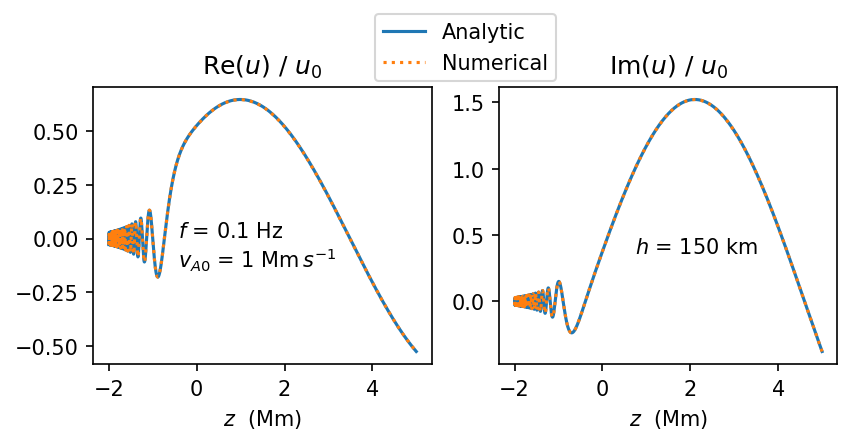
\includegraphics[width=\textwidth]{figures/chapter02/reflection_coefficent_u.png}
    \vspace{-20pt}
    \caption{This figure shows the real and imaginary parts of the normal mode velocity solution. The plots compare the solution calculated using Equation \eqref{eq:reflection_coefficent_u} with the solution calculated numerically. The parameters, $f$, $v_{A0}$, $h$, are listed as well. The code used to make this figure is available on GitHub in the following directory:\newline
    \href{https://github.com/aleksyprok/apkp_thesis/blob/main/Python/Chapter2/reflection_coefficent_u.py}{$\rightarrow$ Python/Chapter2/reflection\_coefficent\_u.py}}
    \vspace{-10pt}
    \label{fig:reflection_coefficent_u}
\end{figure}

In Figure \ref{fig:reflection_coefficent_u} we plot the real and imaginary components of $u$. It suggests that the solution given by Equation \eqref{eq:reflection_coefficent_u} is probably accurate as it agrees with the numerical solution. The numerical solution was calculated using a Runge-Kutta algorithm. More precisely, we used \texttt{solve\_ivp} from \citet{SciPy2020}. We initialised the code with the values of $u$ and $\dv*{u}{z}$ at $z=z_{min}$ using Equations \eqref{eq:reflection_coefficent_u} and \eqref{eq:reflection_coefficent_du_dz}. In the plots we let $h=150\si{.km}$, this value is used in for example \citet{Hollweg1984b}. Note that, if the mean mass of a molecule is given by $m_p/2$, $g_\odot$ is given by \eqref{eq:gravitational_acceleration} then from Equation \eqref{eq:pressure_scale_height} we know that
\[h \approx 151\si{.km}\qty(\frac{T}{10^4\si{.K}}).\]
We used a frequency of $f=0.1\si{.Hz}$, from Figure \ref{fig:power_spectrum_morton} we can see that this is on the high end of the observed frequencies.

\begin{figure}
    \centering
    \vspace{-20pt}
    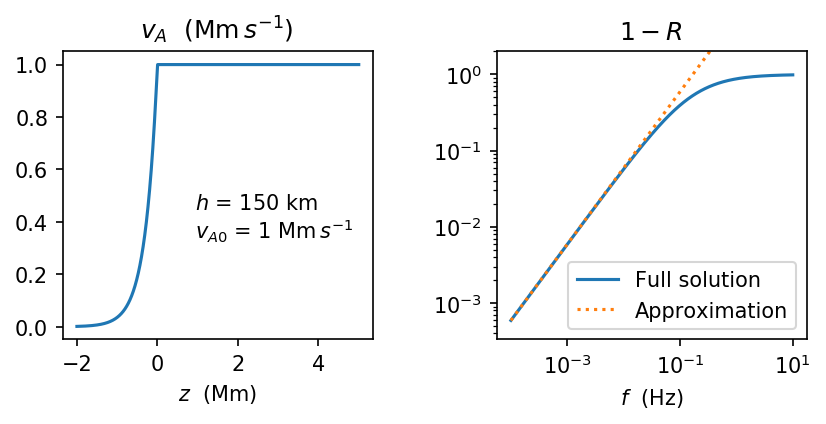
\includegraphics{figures/chapter02/reflection_coefficent.png}
    \vspace{-20pt}
    \caption{This figure shows 1 minus the reflection coefficient, $R$, (right) for the Alfv\'en speed shown on the left. We show the full solution in blue and the approximation, given by Equation \eqref{eq:reflection_coefficent_approximation}, is shown in dotted orange. The code used to make this figure is available on GitHub in the following directory:\newline
    \href{https://github.com/aleksyprok/apkp_thesis/blob/main/Python/Chapter2/reflection_coefficent_u.py}{$\rightarrow$ Python/Chapter2/reflection\_coefficent\_u.py}}
    \vspace{-10pt}
    \label{fig:reflection_coefficent}
\end{figure}

We are mainly interested in the reflection coefficient which we define as 
\begin{equation}
    R = \abs{\frac{c_4}{u_0}}.
\end{equation}
Note that
\begin{equation}
    \bar{H}_0^{(2)}(\xi_0) = H_0^{(1)}(\xi_0),
\end{equation}
and the Wronskian, $W\qty(H_0^{(1)},H_0^{(2)})(\xi)$, is given by
\begin{equation}
    W\qty(H_0^{(1)},H_0^{(2)})(\xi)=H_0^{(1)}H_0'^{(2)}-H_0'^{(1)}H_0^{(2)}=-\frac{4i}{\pi \xi}
\end{equation}
therefore,
\begin{equation}
    \begin{aligned}
        |c_4|^2 &= u_0^2\frac{\abs{H_0^{(2)}}^2 + \abs{H_1^{(2)}}^2 + i\qty(-H_0^{(2)}\bar{H}_1^{(2)}+ H_1^{(2)}\bar{H}_0^{(2)})}{\abs{H_0^{(2)}}^2 + \abs{H_1^{(2)}}^2 + i\qty(H_0^{(2)}\bar{H}_1^{(2)}- H_1^{(2)}\bar{H}_0^{(2)})} \\
        &= u_0^2\frac{\abs{H_0^{(2)}}^2 + \abs{H_1^{(2)}}^2 - 4/(\pi\xi_0)}{\abs{H_0^{(2)}}^2 + \abs{H_1^{(2)}}^2 + 4/(\pi\xi_0)}.
    \end{aligned}
\end{equation}
For typical values, $\xi_0$ is given by
\[\xi_0\approx0.57\times10^{-2}\qty(\frac{h}{150\si{.km}})\qty(\frac{\omega}{6\pi\times10^{-3}\si{.Hz}})\qty(\frac{1\si{.Mm.s^{-1}}}{v_{A0}}).\]
For $\xi_0\ll 1$, $R$ can be approximated as
\begin{equation}
    \label{eq:reflection_coefficent_approximation}
    R = 1 - \pi \xi_0 + O\qty(\xi_0^2).
\end{equation}
1 minus the reflection coefficient and its approximation are plotted in Figure \ref{fig:reflection_coefficent}. It shows that longer wavelength (or lower frequency) waves have larger reflection coefficients. If the wavelength of the wave is longer than the pressure scale height, $h$, then a large fraction of the wave energy will reflect at $z=0$. If the wavelength is shorter than $h$, the waves mostly leak out of the corona into the chromosphere and photosphere.

\section{Leaky loop: general solution}
\label{sec:leaky_loop_general_solution}

This section aims to calculate the general solution for a leaky loop, i.e. a loop where the boundaries' reflection coefficient is less than 1.

Since the loop is leaky, our system's boundary conditions can no longer be given by Equation \eqref{eq:bcs_chap_2}. To precisely define our boundary conditions we introduce a set of variables called Els\"asser variables $\mathcal{Z}^+$, $\mathcal{Z}^-$ which are defined as
\begin{equation}
    \label{eq:elsasser_z}
    \mathcal{Z}^\pm = u \pm v_{A0}\frac{b}{B_0}.
\end{equation}
From Equations \eqref{eq:uy_eqn_linear} and \eqref{eq:by_eqn_linear} we know that
\begin{equation}
    \begin{aligned}
    \pdv{u}{t} &= \frac{v_{A0}^2}{B_0}\pdv{b}{z}, \\
    \frac{v_{A0}}{B_0}\pdv{b}{t} &= v_{A0}\pdv{u}{z}.
    \end{aligned}
\end{equation}
Adding and subtracting the above equations gives
\begin{equation}
    \label{eq:elsasser_advection}
    \pdv{\mathcal{Z}^\pm}{t}\mp v_{A0}\pdv{\mathcal{Z}^\pm}{z}=0,
\end{equation}
respectively. Equation \eqref{eq:elsasser_advection} gives the 1D advection equation for negative propagating and positive propagating waves, respectively, where positive propagating waves travel in the positive $z$-direction. It shows that $\mathcal{Z}^+$ travels in the negative direction and $\mathcal{Z}^-$ travels in the positive direction. We define the boundary conditions as 
\begin{equation}
    \label{eq:bcs_elsasser}
    \begin{aligned}
    \mathcal{Z}^-(-l_z, t) &= 2f_{driv}(t) - R \mathcal{Z}^+(-l_z, t), \\
    \mathcal{Z}^+(l_z, t) &= -R \mathcal{Z}^-(l_z, t) \\
    \end{aligned}
\end{equation}
where $R$ is the reflection coefficient. Note that for $R=1$ we recover Equation \eqref{eq:bcs_chap_2} since $u = (\mathcal{Z}^+ + \mathcal{Z}^-) / 2$. The motivation for these boundary conditions is that each time a wave reaches $\pm l_z$ a fraction $R$ of the amplitude is reflected.

The full solution with the boundary conditions given by \eqref{eq:bcs_elsasser} and initial conditions given by \eqref{eq:initial_condition} is given by
\begin{equation}
    \label{eq:leaky_loop_general_solution}
    \begin{aligned}
    u(z,t) = \sum_{k=0}^m(-1)^kR^kH(\theta_k)f_{driv}(\theta_k),
    \end{aligned}
\end{equation}
where $\theta_k$ is given by Equation \eqref{eq:theta_k} and $m$ is given by Equation \eqref{eq:m} which for convenience we write again here
\begin{equation}
    \tag{\ref{eq:theta_k}}
    \theta_k=t-(-1)^k\frac{z}{v_{A0}}-\frac{(2k+1)l}{v_{A0}},
\end{equation}
\begin{equation}
    \tag{\ref{eq:m}}
    m = \left\lfloor\frac{t v_{A0}}{L_z}\right\rfloor.
\end{equation}
Note that this is almost the same as Equation \eqref{eq:closed_loop_general_solution_finite} except a factor $R^k$ has been introduced. From Equation \eqref{eq:by_eqn_linear} we know that $b$ is given by
\begin{equation}
    b(z,t) = -\frac{B_0}{v_{A0}}\sum_{k=0}^mR^kH(\theta_k)f_{driv}(\theta_k).
\end{equation}

\begin{figure}
    \centering
    \vspace{-20pt}
    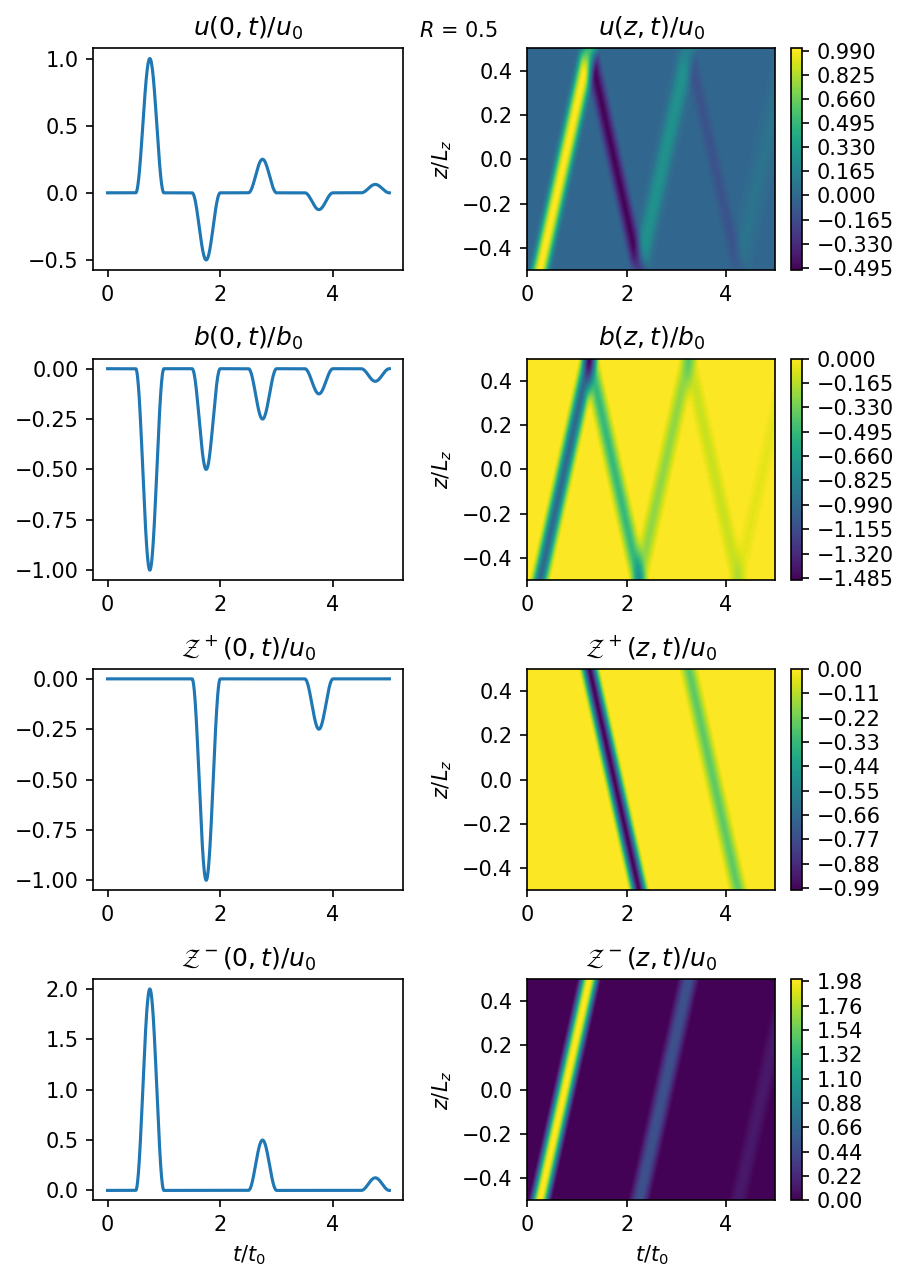
\includegraphics[width=\textwidth,height=0.9\textheight,keepaspectratio]{figures/chapter02/leaky_pulse.png}
    \vspace{-10pt}
    \caption{This figure plots $u$, $b$, $\mathcal{Z}^{+}$, $\mathcal{Z^{-}}$ for the case where $f_{driv}(t)$ is given by Equation \eqref{eq:f_driv_leaky_pulse} and this gives a pulse wave. Here the reflection coefficient is given by $R=0.5$. Note that $b_0$ is given by Equation \eqref{eq:b0}. The code used to make this figure is available on GitHub in the following directory:\newline
    \href{https://github.com/aleksyprok/apkp_thesis/blob/main/Python/Chapter2/leaky_pulse.py}{$\rightarrow$ Python/Chapter2/leaky\_pulse.py}}
    \vspace{-30pt}
    \label{fig:leaky_pulse}
\end{figure}

The solution is plotted in Figure \ref{fig:leaky_pulse} for the case where $f_{driv}$ produces a pulse. The driver is given by
\begin{equation}
    \label{eq:f_driv_leaky_pulse}
    f_{driv} = u_0\begin{cases}
    \sin^2(2\pi t / t_0), & t \le t_0 / 2,  \\
    0, & t > t_0 / 2,
    \end{cases}
\end{equation}
where $t_0$ is given by Equation \eqref{eq:t0}. The reflection coefficient is given by $R=0.5$. It shows that the wave's amplitude reduces by a factor $R$ each time it reflects at one of the boundaries. The figure confirms that $\mathcal{Z}^-$ does indeed correspond to positive propagating waves and $\mathcal{Z}^+$ corresponds to negative propagating waves.

\begin{figure}
    \centering
    \vspace{-20pt}
    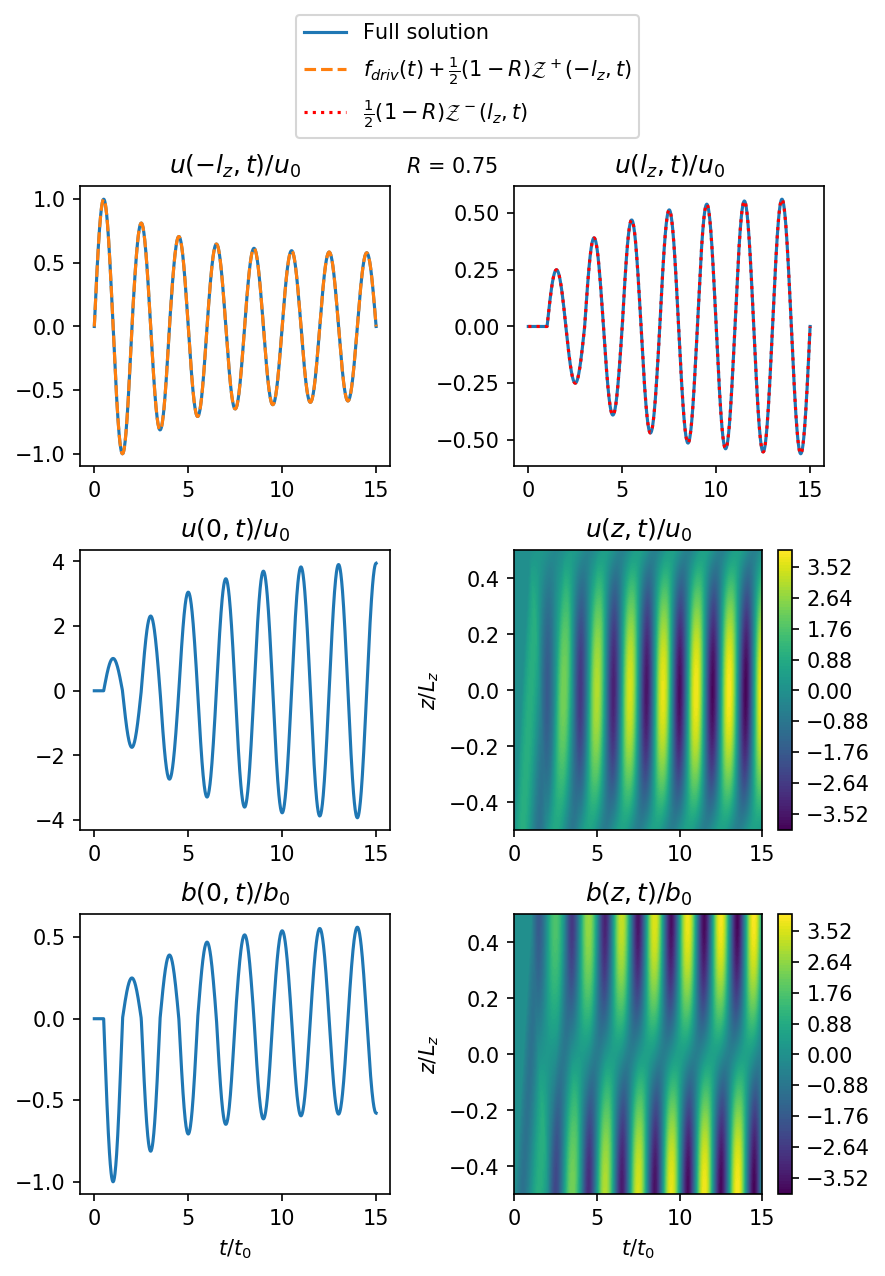
\includegraphics[width=\textwidth,height=0.85\textheight,keepaspectratio]{figures/chapter02/leaky_wave.png}
    \vspace{-10pt}
    \caption{This figure plots $u$, $b$, $\mathcal{Z}^{+}$, $\mathcal{Z^{-}}$ for the case where $f_{driv}(t)$ is given by Equation \eqref{eq:f_driv_leaky_wave} and this gives a continuous sinusoidal wave. Here the reflection coefficient is given by $R=0.75$. The top row show plots at $z=-l_z$ (left) and $z=l_z$ (right) and they show that the boundary conditions given by Equation \eqref{eq:bcs_elsasser} are satisfied. The code used to make this figure is available on GitHub in the following directory:\newline
    \href{https://github.com/aleksyprok/apkp_thesis/blob/main/Python/Chapter2/leaky_wave.py}{$\rightarrow$ Python/Chapter2/leaky\_wave.py}}
    \vspace{-30pt}
    \label{fig:leaky_wave}
\end{figure}

Figure \ref{fig:leaky_wave} plots the solution for the case where $f_{driv}$ produces a continuous sinusoidal wave. The driver is given by
\begin{equation}
    \label{eq:f_driv_leaky_wave}
    f_{driv} = u_0 \sin(\pi t / t_0).
\end{equation}
It confirms that the boundary conditions are satisfied since Equation \eqref{eq:bcs_elsasser} implies that
\begin{equation}
\begin{aligned}
    u(-l_z,t) &= f_{driv}(t)+\frac{1}{2}(1-R)\mathcal{Z}^+(-l_z,t) \\
    u(l_z,t) &= \frac{1}{2}(1-R)\mathcal{Z}^-(l_z,t). \\
\end{aligned}
\end{equation}
The plots also suggest that waves saturate at a maximum amplitude despite being driven at the resonant frequency for $R<1$. For $t\rightarrow \infty$ the amplitude of the waves saturates and the system oscillates at the driver frequency and we say it is at steady-state. The period in which the amplitude of the wave is changing is called the transient phase.

\section{Leaky loop: steady state solution}
\label{sec:leaky_loop_steady_state_solution}

At the end of the previous section, we suggested that for a continuous sinusoidal driver and $R<1$, the system will evolve towards a steady-state. At steady-state, the system oscillates at the driver frequency, and the amplitude saturates at a constant value. This section aims to prove that this is true for all frequencies and calculate the wave's amplitude at steady-state for a continuous sinusoidal driver.

Let $f_{driv}$ be given by
\begin{equation}
    \tag{\ref{eq:driver_sinusoidal}}
    f_{driv}(t)=u_0\exp(i\omega t).
\end{equation}
We seek the solution for $t \rightarrow\infty$, therefore, from Equation \eqref{eq:leaky_loop_general_solution}, we know that $u$ is given by
\[
    \begin{aligned}
    u(z,t) &= u_0\sum_{k=0}^\infty(-1)^kR^kH(\theta_k)\exp(i\omega\theta_k) \\
=&u_0\exp(i\omega[t-z/v_{A0}-l_z/v_{A0}])\frac{1}{2}\sum_{k=0}^{\infty}(1+(-1)^k)R^k\exp(-2i\omega l_z/v_{A0})^k-\\
&u_0\exp(i\omega[t+z/v_{A0}-l_z/v_{A0}])\frac{1}{2}\sum_{k=0}^{\infty}(1-(-1)^k)R^k\exp(-2i\omega l_z/v_{A0})^k. \\
    \end{aligned}
\]
Using the formula for an infinite geometric series the steady state solution is given by,
\begin{equation}
    \label{eq:leaky_steady_state_u}
    u(z,t) = u_0\exp(i\omega[t - l_z/v_{A0}])\frac{\exp(-i\omega z / v_{A0})-r\exp(i\omega z / v_{A0})}{1-r^2},
\end{equation}
provided $R<1$, where
\begin{equation}
    \label{eq:lower_case_r}
    r = R\exp(-2i\omega l_z / v_{A0}).
\end{equation}
Using Equation \eqref{eq:by_eqn_linear} the magnetic field is given by
\begin{equation}
    \label{eq:leaky_steady_state_b}
    b= -\frac{B_0u_0}{v_{A0}}\exp(i\omega[t - l_z/v_{A0}])\frac{\exp(-i\omega z / v_{A0})+r\exp(i\omega z / v_{A0})}{1-r^2}
\end{equation}

\begin{figure}
    \centering
    \vspace{-20pt}
    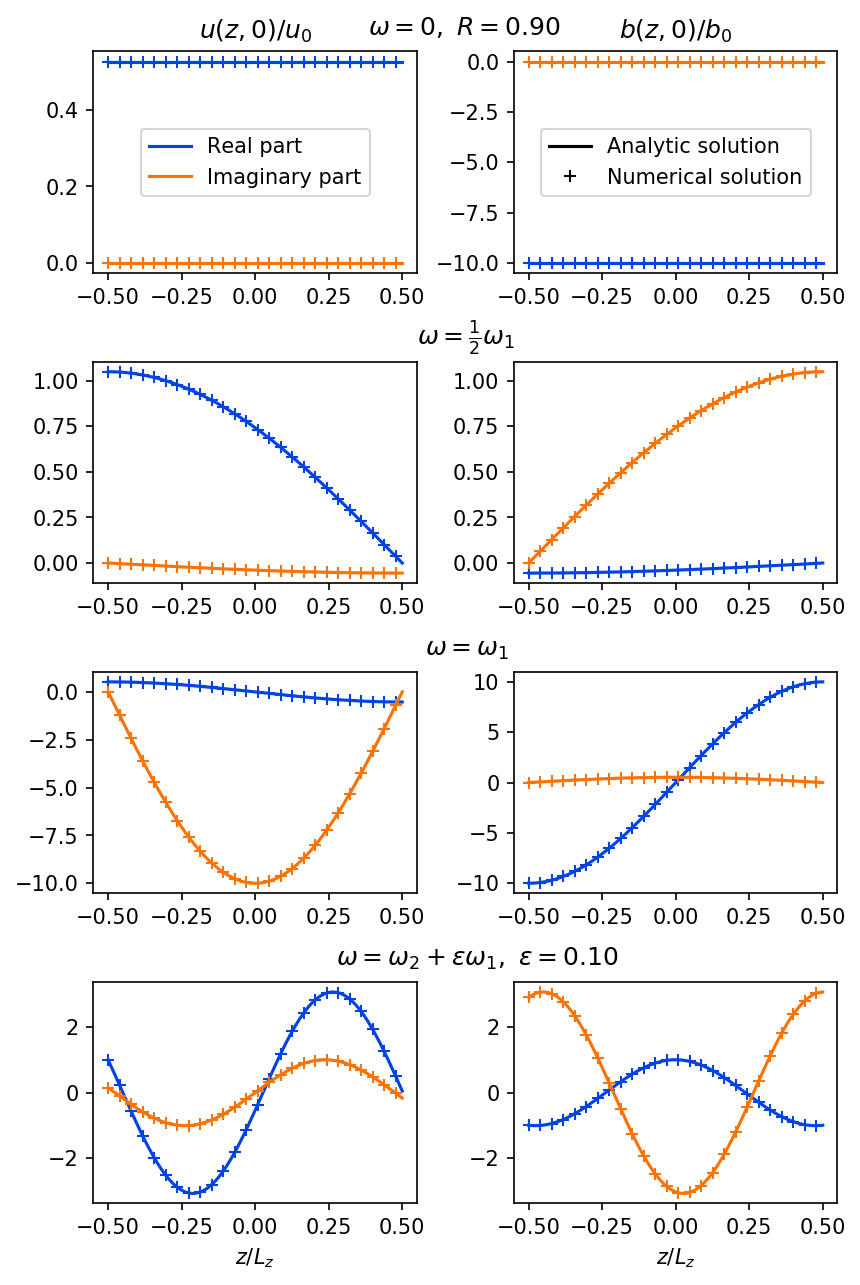
\includegraphics[width=\textwidth,height=0.85\textheight,keepaspectratio]{figures/chapter02/steady_state_soln_along_z.png}
    \vspace{-10pt}
    \caption{This figure shows plots of the steady state velocity (left) and magnetic field (right) along $z$. In each row a different frequency driver is used. The analytic solutions (solid line) were calculated using Equations \eqref{eq:leaky_steady_state_u} and \eqref{eq:leaky_steady_state_b}. The numerical solutions (+ symbols) were calculated by solving the boundary value problem described by Equation \eqref{eq:numerical_elssasser_eqn} using \texttt{solve\_bvp} in \citet{SciPy2020}. The code used to make this figure is available on GitHub in the following directory:\newline
    \href{https://github.com/aleksyprok/apkp_thesis/blob/main/Python/Chapter2/steady_state_soln.py}{$\rightarrow$ Python/Chapter2/steady\_state\_soln.py}}
    \vspace{-30pt}
    \label{fig:steady_state_soln_along_z}
\end{figure}

We can also calculate the steady-state solution via a numerical approach. This is useful to check that the analytic solution is correct. We seek the steady-state solution where the whole system oscillates at the driver frequency. Therefore, we can assume that the time dependence is given by $\exp(i\omega t)$. Assuming the time dependence implicitly, we can simplify the PDEs given by Equation \eqref{eq:elsasser_advection} into the following ODEs,
\begin{equation}
    \label{eq:numerical_elssasser_eqn}
    \dv{Z^{\pm}}{z}=\pm i\frac{\omega}{v_{A0}}Z^{\pm}.
\end{equation}
Note that this system of ODEs is coupled due to the boundary conditions given by Equation \eqref{eq:bcs_elsasser}. We can solve this boundary value problem numerically using \texttt{solve\_bvp} in \citet{SciPy2020}. In Figure \ref{fig:steady_state_soln_along_z} we plot the real and imaginary parts of the steady state velocity, $u$, and magnetic field, $b$ as a function of $z$ at $t=0$. For each plot $R=0.9$. The top-row plots the solution for $\omega=0$. The second row plots the solution for $\omega=\omega_1/2$, where $\omega_1$ is the fundamental resonant frequency, see Equation \eqref{eq:chap_2_omega_n}. The third row plots the solution for $\omega = \omega_1$. Finally, the last row plots the solution for $\omega=\omega_2 + 0.1\omega_1$. They show that the numerical and analytic solutions agree and this suggests that Equations \eqref{eq:leaky_steady_state_u} and \eqref{eq:leaky_steady_state_b} are accurate.

\begin{figure}
    \centering
    \vspace{-20pt}
    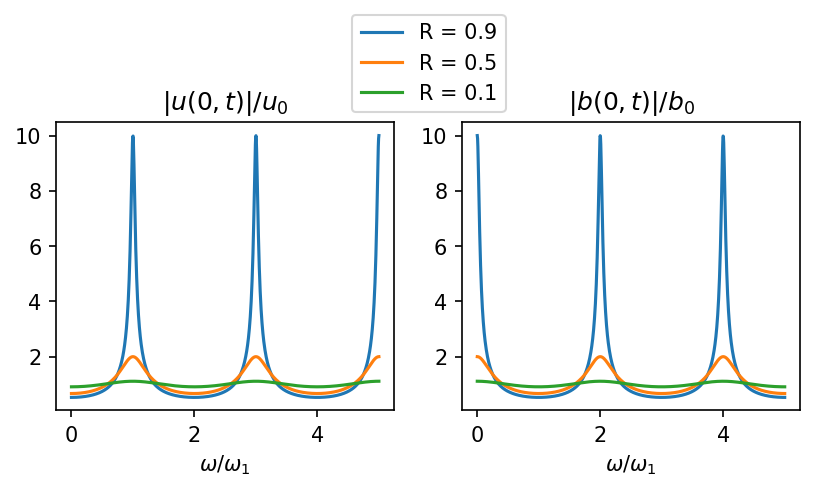
\includegraphics[width=\textwidth,height=0.9\textheight,keepaspectratio]{figures/chapter02/steady_state_soln_at_z=0.png}
    \vspace{-30pt}
    \caption{This figure shows plots of the absolute value of the velocity and magnetic field at $z=0$ as a function of the driver frequency, $\omega$, for $R=0.9$, 0.5 and 0.1. The absolute values were calculated using Equations \eqref{eq:abs_leaky_steady_state_u} and \eqref{eq:abs_leaky_steady_state_b}. Note that $b_0$ is given by Equation \eqref{eq:b0}. The code used to make this figure is available on GitHub in the following directory:\newline
    \href{https://github.com/aleksyprok/apkp_thesis/blob/main/Python/Chapter2/steady_state_soln_at_z\%3D0.py}{$\rightarrow$ Python/Chapter2/steady\_state\_soln\_at\_z=0.py}}
    \label{fig:steady_state_soln_at_z=0}
\end{figure}

At $z=0$, Equation \eqref{eq:leaky_steady_state_u} can be simplified to give
\begin{equation}
    \label{eq:leaky_steady_state_u_z=0}
    u(0,t) = u_0\exp(i\omega[t - l_z/v_{A0}])\frac{1}{1+r},
\end{equation}
and Equation \eqref{eq:leaky_steady_state_b} gives
\begin{equation}
    \label{eq:leaky_steady_state_b_z=0}
    b(0,t) = -\frac{B_0u_0}{v_{A0}}\exp(i\omega[t - l_z/v_{A0}])\frac{1}{1-r}.
\end{equation}
Therefore, the absolute value of $u(0,t)$ is given by
\begin{equation}
    \label{eq:abs_leaky_steady_state_u}
    \abs{u(0,t)} = \frac{u_0}{\sqrt{R^2+2R\cos(2\omega l_z / v_{A0})+1}},
\end{equation}
and the absolute value of $b(0,t)$ is given by
\begin{equation}
    \label{eq:abs_leaky_steady_state_b}
    \abs{b(0,t)} = \frac{B_0 u_0 / v_{A0}}{\sqrt{R^2-2R\cos(2\omega l_z / v_{A0})+1}}.
\end{equation}
In Figure \ref{fig:steady_state_soln_at_z=0} we use Equations \eqref{eq:abs_leaky_steady_state_u} and \eqref{eq:abs_leaky_steady_state_b} to plot the absolute value of the steady state  velocity, $u$ and magnetic field $b$ at $z=0$ as function of the driver frequency, $\omega$. The values are shown for $R=0.9$, 0.5 and 0.1. It shows that as $R\rightarrow 1$ then the absolute value goes to infinity at the resonant frequencies.

\section{Open loop: phase mixing}
\label{sec:phase_mixing}

This chapter has modelled the plasma as ideal, i.e. we have neglected resistivity and viscosity. We justify this because the Reynolds numbers for observed wavelengths is much greater than unity, see Equations \eqref{eq:visc_reynolds_number} and \eqref{eq:mag_reynolds_number}. This section introduces a mechanism, namely phase mixing, that can generate very short length-scales, resulting in very small Reynolds numbers. Phase mixing is the process where gradients perpendicular to the field build-up due to Alfv\'en waves propagating on field lines with a spatial gradient in Alfvén travel time. Where the Alfv\'en travel time is the time it takes for Alfv\'en waves to propagate along the loop over a given distance. To illustrate phase mixing, we calculate the time evolution of driven Alfv\'en waves propagating in an open domain where $v_A=v_A(x)$.

We introduce an $x$-dependence, i.e. let
\[u = u(x,z,t),\quad b = b(x,z,t),\quad v_{A0} = v_A(x).\]
Note that the magnetic field is still given by Equation \eqref{eq:background_field}.
We impose a driver at $z=0$ and impose open boundary conditions. Hence, $\mathcal{Z}^+=0$, i.e. the solution can only contain solutions propagating in the positive $z$-direction. Therefore, $u=\mathcal{Z}^-/2$, and substituting this into Equation \eqref{eq:elsasser_advection} gives
\begin{equation}
    \label{eq:advection_positive}
    \pdv{u}{t}+v_A(x)\pdv{u}{z}=0.
\end{equation}
We aim to solve Equation \eqref{eq:advection_positive} with the following initial condition
\begin{equation}
    u(x,z,0) = 0,
\end{equation}
and boundary condition
\begin{equation}
    u(x,0,t) = f_{driv}(x,t).
\end{equation}
This has the solution
\begin{equation}
    u(x,z,t) = H\qty(t - \frac{z}{v_A(x)})f_{driv}\qty(x,t - \frac{z}{v_A(x)}).
\end{equation}

Consider the case where
\begin{equation}
    f_{driv}(x, t) = u_0\sin(\omega t),
\end{equation}
and
\begin{equation}
    v_A(x) = v_{A0}\qty(1+\frac{x}{L_x}),
\end{equation}
where $x > -L_x$.
Hence,
\begin{equation}
    u(x,z,t) = u_0H\qty(t - \frac{z}{v_A(x)})\sin\qty[\omega\qty(t - \frac{z}{v_A(x)})].
\end{equation}

\begin{figure}
    \centering
    \vspace{-20pt}
    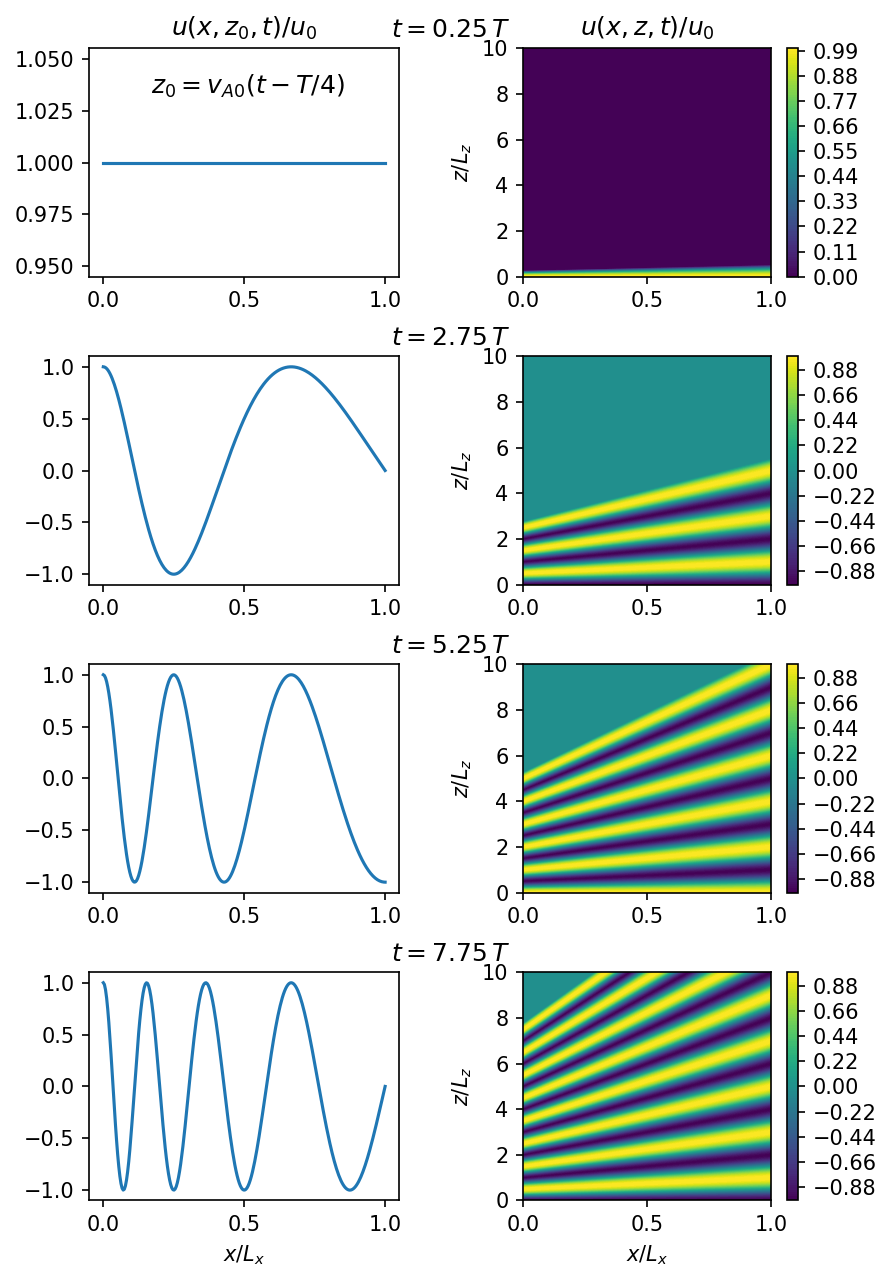
\includegraphics[width=\textwidth,height=0.85\textheight,keepaspectratio]{figures/chapter02/phase_mixing.png}
    \vspace{-10pt}
    \caption{This figure shows snapshots of the velocity, where each row corresponds to a different time. The left side plots the velocity as a function of $x$ at $z=z_0$, where $z_0$ is given by the expression in the top-left plot. The right side shows a contour plot of the velocity as a function of $x$ and $z$. The code used to make this figure is available on GitHub in the following directory:\newline
    \href{https://github.com/aleksyprok/apkp_thesis/blob/main/Python/Chapter2/phase_mixing.py}{$\rightarrow$ Python/Chapter2/phase\_mixing.py}}
    \vspace{-30pt}
    \label{fig:chap_2_phase_mixing}
\end{figure}

We plot this solution in Figure \ref{fig:chap_2_phase_mixing}. It shows the velocity at different snapshots. Note that in Figure \ref{fig:chap_2_phase_mixing}
\[T=\frac{2\pi}{\omega},\ L_z = \frac{2\pi}{\omega}v_{A0}.\]
The top row shows the solution at $t=T/4$, the second row is at $t = 11T/4$, the third row is at $t = 21 T/4$ and the bottom row is at $t = 31 T/4$. The left side shows plots along $x$ at $z=z_0$ where $z_0$ is given by
\[z_0 = v_{A0}\qty(t - \frac{T}{4}).\]
The right side shows contour plots of the velocity as a function of $x$ and $z$. They show that the length-scale in $x$ gets shorter as the wave propagates further along. Consider the plots on the left side, the top plot is equal to a constant value in $x$, we think of this as a curve with only one peak, the second plot has two peaks, the third plot has three peaks, and the bottom plot has four peaks. To quantify the rate at which the length-scales decrease, consider the following.
Assume, $t>z/v_A(x)$, hence,
\begin{equation}
    u(x,z,t) = u_0\sin\qty[\omega\qty(t - \frac{z}{v_A(x)})].
\end{equation}
Taking the $x$-derivative gives
\begin{equation}
    \label{eq:phase_mixing_du_dx}
    \pdv{u}{x} = u_0\omega \dv{v_A}{x}\frac{z}{v_A^2}\cos\qty[\omega\qty(t - \frac{z}{v_A(x)})].
\end{equation}
This shows that the gradients in $x$ grow linearly with $z$.

\section{Discussion and conclusions}

In this chapter, our goal was to introduce some key properties of ideal footpoint driven Alfv\'en waves relevant for the rest of this thesis. In Section \ref{sec:chap_2_closed_loop_general_soln} we showed how d'Alambert's formula and a method of images approach can be used to calculate the general solution in a closed loop. In Section \ref{sec:closed_loop_sinusoidal_solution} we showed that if the driver is of the form $\exp(i\omega t)$ then the general solution can be simplified using the geometric series formula. We showed that if the driving frequency is equal to one of the natural frequencies, i.e. $\omega = \omega_n$, (where $\omega_n$ is given by Equation \ref{eq:chap_2_omega_n}), then the energy of the solution will grow quadratically and ubounded in time. If $\omega\ne\omega_n$ then the solution will oscillate about a finite value. We showed in Figures \ref{fig:case_where_omega=omega_n_u} and \ref{fig:case_where_omega=omega_n_b} that if the driver frequency equals the the zeroth harmonic, $\omega=\omega_0=0$, then then only the magnetic energy grows to infinity and the kinetic energy oscillates about a finite value. Whereas, for the other harmonics, i.e. $\omega_n$ for $n\ge1$, both the kinetic and magnetic kinetic energy grows to infinity. If $\omega=\omega_0$ then the velocity of the driver never changes sign, which stretches the magnetic field, resulting in a large build-up of magnetic energy for a small amount of kinetic energy. If $\omega=\omega_n$ for $n\ge 1$ then a standing wave is set up and this has approximately equal magnetic and kinetic energy (averaged over one wave period).

The sinusoidal driver is useful because it is relatively easy to calculate the exact solution. In reality, the photosphere will excite a range of frequencies, and this can be modelled by superimposing sinusoidal solutions via a Fourier series approach. In Section \ref{sec:closed_loop_random_driver} we calculate the solution for a broadband driver, i.e. a driver which excites a broad range of frequencies. In Section \ref{sec:chap_2_driven_harmonic_oscillator} we assumed a Fourier series solution in $z$ to convert the Alfv\'en wave equation, a PDE, into a set of ODEs for a driven harmonic oscillator. We calculated the exact solution for a red noise force and white noise force driver (in Section \ref{sec:noisy_force}, we define red and white noise). We also estimated the solutions with a red and white noise force driver by approximating them with a finite Fourier series. Figure \ref{fig:noisy_driver} compares the exact and approximate solutions and show they converge as the number of harmonics increases. The error shows a steep reduction if the resonant harmonic is excited. Note that red and white noise force drivers are unphysical because they have an infinite variance. However, they are still useful concepts because it is simple to calculate an exact analytic solution using a red and white noise force driver (see Section \ref{sec:noisy_force}). Moreover, the approximate solutions in Figure \ref{fig:noisy_driver} have a finite variance and show similar results. Results from Section \ref{sec:closed_loop_random_driver} show that the variance and energy grow linearly when either a red noise or white noise force driver is used. Whereas in Section \ref{sec:closed_loop_sinusoidal_solution} we showed that if a sinusoidal driver is used with $\omega=\omega_n$, the energy grows quadratically with time.

In Sections \ref{sec:chap_2_closed_loop_general_soln}-\ref{sec:closed_loop_random_driver} we used line-tied boundary conditions. These boundary conditions are motivated by the fact that the chromosphere is significantly denser than the corona. However, despite the large change in density, a small fraction of the waves will leak from the corona into the chromosphere. In Section \ref{sec:leaky_loop_reflection_coefficent} we calculate an estimate for the reflection coefficient using a similar model to that used in \citet{Hollweg1984b}. Figure \ref{fig:reflection_coefficent_u} plots the reflection coefficent as a function of frequency. It shows that the higher the frequency (i.e. shorter wavelength), the more the waves leak out of the corona. In Section \ref{sec:leaky_loop_general_solution} we calculate the general solution for waves in a leaky loop. We show that the solution evolves towards a state where the whole system oscillates at the driver frequency, and this is called the steady-state solution. In Section \ref{sec:leaky_loop_steady_state_solution} for a sinusoidal driver and confirm it numerically in Figure \ref{fig:steady_state_soln_along_z}. Figure \ref{fig:steady_state_soln_at_z=0} shows that the steady-state solution's amplitude is largest at the resonant frequencies and tends to infinity as the reflection coefficient, $R$, goes to 1. Note that the timescale to reach steady-state also grows to infinity as $R\rightarrow 1$, and so we recover the closed-loop solution as $R\rightarrow 1$.

Finally, in Section \ref{sec:phase_mixing} we introduce a phenomenon called phase mixing. Figure \ref{fig:chap_2_phase_mixing} shows if neighbouring field lines have different Alfv\'en speeds, this can result in Alfv\'en waves moving out of phase with their neighbours as they evolve. This results in the growth of steep gradients perpendicular to the field, which may be important in coronal heating, we discuss this further in the next chapter.

% To prove that the velocity is continuous we first show that the tangential component of the electric field, $\vec{E}$, is continuous. We apply Stokes' theorem to Faraday's law, Equation \eqref{eq:faradays_law}, to give the integral form of Faraday's law,
% \[\oint_{\partial S}\vec{E}\cdot d\vec{l} = -\int_S \pdv{\vec{B}}{t}\cdot d\vec{S}.\]
% We choose $S$ as a small rectangle across the interface. This is is illustrated in Figure \ref{fig:curl_e}. The sides perpendicular to the interface have length $h$ above and below the interface. The sides parallel to the interface have length l. Let $h\rightarrow0$, now the area of integration looks like a line, which as zero area. In other words,
% \[\lim_{h\rightarrow 0}\vec{S}=0.\]
% Since $\pdv*{\vec{B}}{t}$ remains finite in this limit, the whole right hand side goes to zero. All that is left is
% \[\oint_{\partial S}\vec{E}\cdot d\vec{l}=0.\]
% Assuming our rectangle is small enough that $E$ is roughly constant, its magnitude can be pulled out of the integral. As the remaining sides to our original rectangle, the $d\vec{l}$ in each region run in opposite directions, so we define one of them as the tangent unit vector, $\vec{t}$, and the other as $-\vec{t}$.
% Let the region $z<0$ be labelled medium 1 and the region $z>0$ be denoted medium 2. Hence,
% \[\vec{E}_2\cdot\vec{t}l-(\vec{E}_1\cdot\vec{t})l=0,\]
% \[\implies (\vec{E}_2-\vec{E}_1)\cdot\vec{t}=0.\]
% Therefore, we have proven that the tangential component of the electric field must be continuous across $z=0$.

% \begin{figure}
%     \centering
%     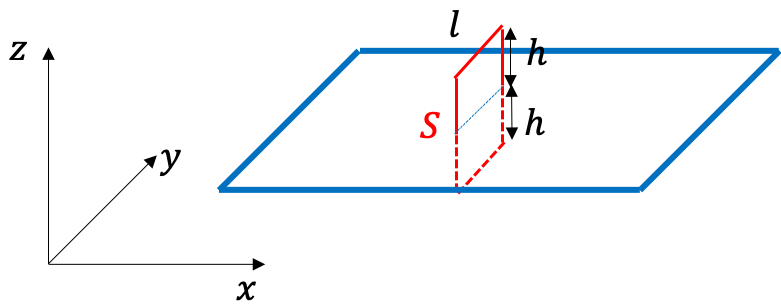
\includegraphics{figures/chapter02/curl_e.png}
%     \caption{This figure illustrates the rectangle, $S$, which is used to prove that the tangential component of the electric field is zero.}
%     \label{fig:curl_e}
% \end{figure}

\chapter{Resistive phase-mixed Alfv\'en waves}
\label{chap:resistive_phase_mixed_alfven_waves}
\section{Introduction}
\label{sec:chap_3_introduction}

At the end of the previous chapter, we introduced a concept called phase-mixing. We saw that very short-length-scales can build up when Alfv\'en waves propagate along field lines with different Alfv\'en travel times. Since each field line has different Alfv\'en travel times, this can lead to waves moving out of phase with their neighbours. This suggests that the ideal assumption we made in the previous chapter may no longer be valid. Moreover, it has been suggested in, for example, \citet{Heyvaerts1983} that phase-mixed Alfv\'en waves could play a significant role in coronal heating.

Phase mixing has been researched extensively since \citet{Heyvaerts1983} first proposed it as a coronal heating mechanism. For example, \citet{Browning1984}, expanded on the \citet{Heyvaerts1983} work related to the Kelvin-Helmholtz instability. They show that standing phase-mixed Alfv\'en waves are unstable to the Kelvin-Helmholtz instability and will undergo a turbulent cascade, leading to enhanced dissipation of energy. In for example, \citet{DeMoortel2002} and \citet{Smith2007} they study phase mixing in a stratified and divergent magnetic field. \citet{Similon1989} and \citet{Howson2019} study phase mixing in a complex magnetic field. \citet{Hood1997,Hood2002} investigate phase mixing in coronal holes and calculate a self-similar solution which enables them to analyse a more general class of solutions. They find that a single pulse decays algebraically rather than exponentially. In \citet{McLaughlin2011a,McLaughlin2013,Prokopyszyn2019a} they study phase mixing of nonlinear Alfv\'en waves near 2D x-type null points. Phase mixing has also been investigated in 3D \citep{Magyar2017} and 3D coronal loops \citep{Pagano2017,Pagano2018}.

In this chapter, we aim to answer whether the phase-mixing of Alfv\'en waves plays an important or negligible role in coronal heating? To help answer this question, we introduce a term called the heating rate per unit of wave energy in a loop, denoted with $\gamma$. We define $\gamma$ as the ratio of the integrated time-averaged heating rate along a loop over the wave energy of the loop, i.e.
\begin{equation}
    \gamma = \frac{\left\langle\int_C \vec{\sigma}_{Brag}:\grad{u} + j^2/\sigma dl\right\rangle}{\frac{1}{2}\left\langle\int_C \rho u^2 + b^2 dl\right\rangle},
\end{equation}
where $C$ is a contour of a given coronal loop and $\langle\rangle$ denotes the time average. Note that $\gamma$ is closely related to the damping coefficient used in the equation to describe damped harmonic oscillators. The equation for a damped harmonic oscillator, with amplitude $x(t)$, is given by
\begin{equation}
    \dv[2]{x}{t}+\gamma_0\dv{x}{t}+\omega_0^2 x = 0.
\end{equation}
Multiplying through by $\dv*{x}{t}$ gives
\begin{equation}
    \dv{}{t}\qty[\frac{1}{2}\qty(\dv{x}{t})^2+\frac{1}{2}\omega_0^2 x] = -\gamma_0 \qty(\dv{x}{t})^2.
\end{equation}
Note that the time average of the potential energy, $\langle \omega_0^2 x^2 / 2 \rangle$, is approximately equal to the time average of the kinetic energy, $\langle (\dv*{x}{t})^2/2\rangle$, therefore, the heating rate over the kinetic and potential energy is given by
\begin{equation}
    \gamma_0 \approx \frac{\gamma_0\langle (\pdv*{x}{t})^2\rangle}{\frac{1}{2}\langle(\pdv*{x}{t})^2+\omega_0^2x^2\rangle}.
\end{equation}
Therefore, $\gamma$ and $\gamma_0$ satisfy very similar definitions, which explains why $\gamma$ is closely related to the waves' damping rate. Note that \citet{Hollweg1984a,Hollweg1984b} uses a very similar idea to $\gamma$ except they use a quantity called the quality factor, from resonance theory, which is approximately given by $\omega / \gamma$, where $\omega$ is the angular frequency of a wave. We focus on using $\gamma$ because it is easier to apply to a system in which multiple frequencies are excited. \citet{Arregui2015} also discusses a similar idea. He argues (through an order magnitude analysis) that phase mixing could take too long to reach the required length scales for the heating rate to become important.

We can estimate the conductive and radiative losses \citep{Withbroe1977} and the wave energy \citep{McIntosh2011,McIntosh2012} in the corona. Using these values, we can approximate the value $\gamma$ needs to satisfy for the conductive and radiative energy losses to be balanced by the viscous and Ohmic dissipation of the observed waves. This gives the required value of $\gamma$ for coronal heating and we will compare it with the value of $\gamma$ predicted by phase-mixing theory. This is how we will test if phase mixing can play a significant role in coronal heating. In Section \ref{sec:chap_3_coronal_heating} we estimate an upper bound for the $\gamma$ predicted by phase-mixing theory by ensuring any simplifications made act to increase the value of $\gamma$. If our upper bound is too small, we can conclude that phase-mixing plays a negligible role in coronal heating. If the upper bound is equal to or larger than the required $\gamma$ then this means phase-mixing could play an important role. However, we would need a more realistic model to know for sure. In this section, we will calculate the required value of $\gamma$ in a closed loop. 

We can estimate the conductive and radiative losses in a closed coronal loop via a theoretical and observational approach. We will first calculate the theoretical energy losses and then check them with the observations given by \citet{Withbroe1977}. If we assume the radiative loss function can be approximated with
\begin{equation}
    Q(T) = \chi T^{-1/2},
\end{equation}
where $\chi=10^{-32}\si{.K^{1/2}.W.m^3}$, then \citet{Priest2014} shows that to maintain a loop with a uniform pressure, $p$, with a uniform heating rate, $H_c$, then $H_c$ must satisfy
\begin{equation}
    \label{eq:coronal_heating_rate_per_unit_volume}
    \begin{aligned}
    H_c &= \frac{7}{8}\frac{\chi}{k_B^2}\frac{p^2}{T_{max}^{5/2}} \\
    &\approx 4.59\times10^{-6}\qty(\frac{\chi}{10^{-32}\si{.K^{1/2}.W.m^3}})\qty(\frac{p}{10^{-2}\si{.Pa}})^2\qty(\frac{10^6\si{.K}}{T_{max}})^{5/2}\si{.W.m^{-3}}
    \end{aligned}
\end{equation}
Table \ref{tab:energy_losses_corona_chromosphere} shows the power losses due to conduction, radiation and solar wind per unit area in the corona. The table gives the power per unit area, whereas our theoretical calculation is per unit volume. Therefore, we need to integrate our theoretical calculation in the radial direction. We model the temperature as uniform in the radial direction and assume the pressure satisfies hydrostatic balance. In other words, we assume that
\begin{equation}
    p=p_0\exp(-r/h),
\end{equation}
where $h$ is the pressure scale height given by Equation \eqref{eq:pressure_scale_height}. Note that for typical values ($m=m_p/2$, $g_{\odot}=274\si{.m^2.s^{-1}}$) the pressure scale height is given by
\begin{equation}
    h = 1.51\times10^8\qty(\frac{T}{10^6\si{.K}})\si{.m}
\end{equation}
Most heating will occur within a height $2h$ of the solar surface, the radius of the Sun is about $0.70\times10^9\si{.m}$ \citep{sun_vital_statistics} which is greater than $h$. Therefore, the error associated with approximating the gravitational field strength as uniform will be small. 
We now need to integrate Equation \eqref{eq:coronal_heating_rate_per_unit_volume} in the radial direction from $r_0$ to $r_1$, where $r_0$ gives the radial coordinate of the base of the corona and $r_1$ gives the coordinate of the top of the corona. The height of the corona is not clearly defined, however, we know that $r_1-r_0\gg h$, therefore, we can approximate $r_1\rightarrow \infty$. Hence, the integral of Equation \eqref{eq:coronal_heating_rate_per_unit_volume} is given by
\begin{equation}
    \begin{aligned}
    \int_{r_0}^\infty H_c \, dr &= \frac{h}{2}\frac{7}{8}\frac{\chi}{k_B^2}\frac{p(r_0)^2}{T_{max}^{5/2}} \\
    &\approx 3.47\times10^{2}\qty(\frac{\chi}{10^{-32}\si{.K^{1/2}.W.m^3}})\qty(\frac{p(r_0)}{10^{-2}\si{.Pa}})^2\qty(\frac{10^6\si{.K}}{T_{max}})^{3/2}\si{.W.m^{-2}}.
    \end{aligned}
\end{equation}
Note that Table \ref{tab:energy_losses_corona_chromosphere}, shows that the energy losses are in the range $[3\times10^2,10^4]\si{.W.m^{-2}}$ and our calculation above lies in this range. Therefore, the theoretical and observational calculations are in agreement. 

In \citet{McIntosh2011,McIntosh2012}, they observe velocity wave amplitudes, $u_0$, in the quiet sun of around $20\si{.km.s^{-1}}$ and in active regions of around $5\si{.km.s^{-1}}$. We can use this data to estimate the corona's wave energy by assuming the time-averaged kinetic energy associated with the waves equals the time-averaged magnetic perturbation energy. This gives a wave energy, $E_{wave}$, of approximately
\begin{equation}
    \label{eq:chap_3_observed_wave_energy}
    \begin{aligned}
    E_{wave} &\approx \rho \langle u_0 \rangle^2 \\
    &\approx10^{-4}\qty(\frac{\rho}{10^{-12}\si{.kg.m^{-3}}}) \qty(\frac{\langle u_0 \rangle}{10^4 \si{.m.s^{-1}}})^2\si{.J.m^{-3}}.
    \end{aligned}
\end{equation}
Therefore, the value $\gamma$ needs to satisfy for the conductive and radiative energy losses to be balanced by the viscous and Ohmic dissipation of the observed waves is given by
\begin{equation}
\label{eq:required_gamma}
\begin{aligned}
    \gamma &= \frac{H_c}{E_{wave}} \\
    &= \frac{7}{2}\frac{\chi}{m_p^2}\frac{\rho}{T_{max}^{1/2}}\frac{1}{\langle u_0\rangle^2} \\
    &\approx1.25\times10^{-1}\qty(\frac{\rho}{10^{-12}\si{.kg.m^{-3}}})\qty(\frac{10^6\si{.K}}{T_{max}})^{1/2}\qty(\frac{10^{4}\si{.m.s^{-1}}}{\langle u_0 \rangle})^2\si{.s^{-1}}.
\end{aligned}
\end{equation}
Therefore, the $\gamma$ predicted by phase-mixing needs to be of the order $10^{-1}\si{.s^{-1}}$ for it provide an important role in coronal heating.

\section{Model and equations}

This chapter will model perturbations on a background medium. We assume the system is linear and we make the same assumptions as described by Equations \eqref{eq:linear_assumotion_v}-\eqref{eq:linear_assumotion_rho}. We will model the background quantities as uniform in $z$. The background magnetic field points in the $z$-direction, i.e.
\begin{equation}
    \tag{\ref{eq:background_field}}
    \vec{B}_0 = B_0\vec{\hat{z}}.
\end{equation}
We model the background Alfv\'en speed to be a function of $x$, i.e. $v_A=v_A(x)$.

We assume the $y$-direction is invariant, i.e. $\pdv*{}{y}=0$. This prevents mode coupling between $u_x$ and $u_y$. \citet{Parker1991} argues that this mode conversion is important and should not be neglected. However, in Chapter \ref{chap:resonant_absorption_in_an_oblique_field} we find that at resonant locations the mode conversion is one-way from fast to Alfv\'en waves. Therefore, the results presented in this chapter are relevant at these resonant locations (which are discussed in greater detail in Chapter \ref{chap:resonant_absorption_in_an_oblique_field}). Some coronal arcades have an approximate invariant direction, and some flux tubes can be azimuthally invariant. Assuming $\pdv*{}{y}=0$ prevents the development of MHD instabilities. In \citet{Heyvaerts1983}, they show that, for $\pdv*{}{y}\ne0$, standing phase-mixed Alfv\'en waves are unstable to the Kelvin-Helmholtz and tearing instabilities. Also, $\pdv*{}{y}=0$ prevents viscous heating due to gradients in the $y$-direction. If we assume $\vec{u}=u(x,y,z,t)\vec{\hat{y}}$ and $\vec{b}=b(x,y,z,t)\vec{\hat{y}}$ then the viscous heating associated with $\vec{W}^{(0)}$ becomes
\begin{equation}
    \eta_0 \vec{W}^{(0)}:\grad{\vec{u}} = \frac{\eta_0}{3}\qty(\pdv{u}{y})^2,
\end{equation}
where $\vec{W}^{(0)}$ is given by Equation \eqref{eq:braginskii_viscous_stress_tensor}.

We solve for the $y$-component of the velocity, given by
\begin{equation}
    \tag{\ref{eq:y_component_of_u}}
    \vec{u}(x,z,t) = u(x,z,t)\vec{\hat{y}},
\end{equation}
and the $y$-component of the perturbed magnetic field, given by
\begin{equation}
    \tag{\ref{eq:y_component_of_b}}
    \vec{b}(x,z,t) = b(x,z,t)\vec{\hat{y}}.
\end{equation}

The $y$-component of the linearised momentum equation, see Equation \eqref{eq:momentum}, with gravity neglected, see Equation \eqref{eq:ignore_gravity}, is given by
\begin{equation}
    \label{eq:chap_3_momentum_eqn1}
    \begin{aligned}
    \pdv{u}{t} &= \frac{v_A^2(x)}{B_0}\pdv{b}{z} + \frac{1}{\rho}\vec{\hat{y}}\cdot\div{\vec{\sigma}_{Brag}} \\
    &\approx\frac{v_A^2(x)}{B_0}\pdv{b}{z} +\frac{\eta_1}{\rho} \pdv[2]{u}{x} + \frac{\eta_2}{\rho} \pdv[2]{u}{z}.
    \end{aligned}
\end{equation}
where $\vec{\sigma}_{Brag}$ is given by Equation \eqref{eq:braginskii_viscous_stress_tensor}, the plasma pressure and magnetic pressure terms are set to zero because the $y$-direction is invariant. Note that when calculating $\div\vec{\sigma}_{Brag}$, we ignored the derivatives associated with the coefficients, $\eta_0,\eta_1, ...$ etc. as we expect our waves to phase mix and so we expect $\abs{\pdv*{u}{x}/u}\gg\abs{\pdv*{\eta_0}{x}/\eta_0}$. The equations above shows that after linearising the Braginskii viscous tensor, the contribution from the parallel component, $\eta_0\vec{W}^{(0)}$, and the drift terms, $\eta_3\vec{W}^{(3)}$, $\eta_4\vec{W}^{(4)}$ is zero. This result and a discussion on the linearised Braginskii viscous stress tensor are given in, for example, \citet{Ruderman2000,Mocanu2008}. Equations \eqref{eq:braginskii_eta_0} to \eqref{eq:braginskii_eta_2} show that $\eta_0$ is usually much greater than $\eta_1$ and $\eta_2$. Equation \eqref{eq:proton_gyrofrequency_times_collision_time} shows that we estimate $\eta_0$ to be a factor $10^{10}$ greater. By linearising the viscous stress tensor we could be neglecting the dominant term. However, this chapter aims to just study just linear waves, in Section \ref{sec:chap_3_coronal_heating} we investigate parameter space in which this linearization is justified. We intend to study phase mixing, which is a concept we introduced in Section \ref{sec:phase_mixing}, so we make another assumption which is to assume $\pdv*{}{x}\gg\pdv*{}{z}$. Therefore, we simplify Equation \eqref{eq:chap_3_momentum_eqn1} further to give
\begin{equation}
    \label{eq:chap_3_momentum_eqn2}
    \pdv{u}{t}=\frac{v_A^2(x)}{B_0}\pdv{b}{z} +\nu\pdv[2]{u}{x},
\end{equation}
where we set $\nu = \eta_1/\rho$ to keep the notation tidy.

The $y$-component of the linearised induction equation, see Equation \eqref{eq:induction_equation}, is given by
\begin{equation}
    \pdv{b}{t} = B_0\pdv{u}{z}+\eta\nabla^2 b - \underbrace{\vec{\hat{y}}\cdot\curl(\frac{1}{n_e e}\vec{j}\cross\vec{B})}_{\text{Hall term}}.
\end{equation}
Like in the previous paragraph, we simplify this equation further by assuming that $\pdv*{}{x}\gg\pdv*{}{z}$ to give 
\begin{equation}
    \label{eq:chap_3_induction}
    \pdv{b}{t} = B_0\pdv{u}{z}+\eta\pdv[2]{b}{x}.
\end{equation}
Note that we have neglected the Hall term because it is dependent on derivatives which are parallel to the background magnetic field. In, for example, \citet{Threlfall2017} they investigate the effects of the Hall term on phase mixing. They find that the hall terms' introduction causes wave dispersion which reduces the heating rate per unit of wave energy, $\gamma$. We aim to show that linear phase mixed Alfv\'en waves at observed wavelengths have an insufficient $\gamma$ to heat the corona. Therefore, if $\gamma$ is insufficient without the Hall term, we know it must be insufficient with the Hall term.

Substituting Equation \eqref{eq:chap_3_induction} into the time derivative of Equation \eqref{eq:chap_3_momentum_eqn2} gives
\[\pdv[2]{u}{t}=v_A^2(x)\pdv[2]{u}{z}+v_A^2(x)\pdv[2]{}{x}\qty(\frac{\eta}{B_0}\pdv{b}{z})+\nu\pdv{}{t}\pdv[2]{u}{x}.\]
Note that
\[\begin{aligned}
\pdv[2]{}{x}\qty(\frac{\eta}{B_0}\pdv{b}{z}) &= \pdv[2]{}{x}\qty[\frac{\eta}{v_A^2(x)}\qty(\pdv{u}{t} - \nu \pdv[2]{u}{x})] \\
&\approx \frac{\eta}{v_A^2(x)}\pdv{}{t}\pdv[2]{u}{x},
\end{aligned}\]
where we assume that $\eta$ and $\nu$ are small factors such that their products are negligible. Moreover, we assume that $\abs{\pdv*{u}{x}/u}\gg\abs{\pdv*{v_A}{x}/v_A}$ and so we get the approximation above. Using the above two equations we get
\begin{equation}
    \label{eq:wave_diffusion_equation}
    \pdv[2]{u}{t}-v_A^2(x)\pdv[2]{u}{z}= (\eta+\nu)\pdv{}{t}\pdv[2]{u}{x}.
\end{equation}

Equation \eqref{eq:chap_3_momentum_eqn2} can be written as
\[\pdv{u}{t}=v_A(x)\pdv{\hat{b}}{z}+\nu\pdv[2]{u}{x},\]
where
\begin{equation}
    \hat{b}(x,z,t) = \frac{v_A(x)}{B_0}b(x,z,t).
\end{equation}
Also if we assume $\abs{\pdv*{b}{x}/b}\gg\abs{\pdv*{v_A}{x}/v_A}$ then we can approximate Equation \eqref{eq:chap_3_induction}, multiplied by $v_A(x)/B_0$ as 
\[\pdv{\hat{b}}{t}=v_A(x)\pdv{u}{z}+\eta\pdv[2]{\hat{b}}{x}.\]
Combining the above equations gives
\begin{equation}
    \label{eq:advection_diffusion_elsasser}
    \pdv{\mathcal{Z}^\pm}{t} \mp  v_A(x)\pdv{\mathcal{Z}^\pm}{z} = \nu_+ \pdv[2]{Z^\pm}{x} + \nu_-\pdv[2]{Z^\mp}{x},
\end{equation}
with $Z^{\pm}$ is given by 
\begin{equation}
    \tag{\ref{eq:elsasser_z}}
    \mathcal{Z}^\pm(x,z,t) = u(x,z,t) \pm \frac{v_A(x)}{B_0}b(x,z,t),
\end{equation}
and $\nu_{\pm}$ is given by
\begin{equation}
    \nu_\pm = \frac{1}{2}(\eta\pm\nu),
\end{equation}
where we assumed that $\abs{\pdv*{b}{x}/b}\gg\abs{\pdv*{v_A}{x}/v_A}$.

In this chapter, we will solve the above equations for various boundary conditions. In Section \ref{sec:chap_3_open_loop} we solve the above equations for the case where the boundaries are open, in Section \ref{sec:chap_3_closed_loop} we consider a closed-loop and in Section \ref{sec:chap_3_leaky_loop} we study a leaky loop. In all sections, we will have a driver at the bottom boundary ($z=0$) given by
\begin{equation}
    \label{eq:driver_chap_3}
    \begin{aligned}
    u(x,0,t) &= f_{driv}(x,t) \\
    &= f_0\exp(i\omega t).
    \end{aligned}
\end{equation}
We will impose Neumann boundary conditions in $x$, i.e.
\begin{equation}
    \label{eq:neumann_bcs_chap_3}
    \left.\pdv{u}{x}\right|_{x=x_{min}}=\left.\pdv{u}{x}\right|_{x=x_{max}}=0.
\end{equation}
Our initial conditions are
\begin{equation}
    u(x,z,0) = b(x,z,0) = 0.
\end{equation}
For our numerical solutions, the background Alfv\'en speed is given by
\begin{equation}
    \label{eq:background_vA_chap_3}
    v_A(x) = v_{A0}\qty[1 + \frac{x}{a_0}],
\end{equation}
however, for our analytic solutions we will assume the more general form, namely, $v_A=v_A(x)$.

We seek the steady-state solution, where the solution oscillates at the driver frequency. Therefore, we assume a time-dependence of the form $\exp(i\omega t)$ implicitly. Therefore,
Equation \eqref{eq:wave_diffusion_equation} can be written as
\begin{equation}
    \label{eq:method_of_lines_eqn_u}
    \boxed{-i\omega(\eta+\nu)\pdv[2]{u}{x} = \omega^2u + v_A^2\pdv[2]{u}{z},}
\end{equation}
and Equation \eqref{eq:advection_diffusion_elsasser} gives
\begin{equation}
    \label{eq:chap_3_method_of_lines_eqn}
     \boxed{\pdv{\mathcal{Z}^\pm}{z} = \frac{1}{v_A(x)}\qty{\pm i\omega Z^{\pm} + \nu_+ \pdv[2]{Z^\pm}{x} + \nu_-\pdv[2]{Z^\mp}{x}}.}
\end{equation}

\section{Open loop}
\label{sec:chap_3_open_loop}

This section aims to calculate solution to Equation \eqref{eq:chap_3_method_of_lines_eqn} analytically and numerically, for an open loop. We assume the loop contains only waves propagating in the positive $z$-direction so $\mathcal{Z}^+=0$.

\subsection{Analytic solution}

To solve Equation \eqref{eq:chap_3_method_of_lines_eqn} analytically we will use the method of multiple scales, where $\eta+\nu$ gives the small parameter. Since $\mathcal{Z}^+=0$ $\implies$ $u = \mathcal{Z}^{-}/2$. Substituting this into Equation \eqref{eq:chap_3_method_of_lines_eqn} gives
\begin{equation}
    \pdv{u}{z}+ik_z(x)u=\frac{\eta+\nu}{2v_A(x)}\pdv[2]{u}{x},
\end{equation}
where
\begin{equation}
    k_z(x) = \frac{\omega}{v_A(x)}.
\end{equation}
We assume $u(x,z)$ takes the form of the following asymptotic series
\begin{equation}
    u(x,z_0,z_1) = u_0(x,z,\epsilon z) + \epsilon u_1(x,z,\epsilon z) + \epsilon^2 u_2(x,z,\epsilon z) + ...\,.
\end{equation}
where $u$ has a shorter length-scale dependence, $z_0$, given by
\begin{equation}
    z_0 = z
\end{equation}
and a longer length-scale dependence, $z_1$, given by
\begin{equation}
    z_1 = \epsilon z.
\end{equation}
The zeroth order equation is given by
\begin{equation}
    \pdv{u_0}{z}+ik_z(x)u_0=0.
\end{equation}
Solving with the boundary condition,
\begin{equation}
    u(x,0)=f_0,
\end{equation}
gives
\begin{equation}
    \label{eq:u_0_short_timescale}
    u_0(x,z,z_1) = f_0\exp[-ik_z(x)z]A(z_1).
\end{equation}
Note that
\begin{equation}
    \pdv{u}{z} = \pdv{u}{z_0} + \epsilon \pdv{u}{z_1}.
\end{equation}
Hence, the first order equation is given by
\begin{equation}
    \pdv{u_1}{z}+ik_z(x)u_1 = -\pdv{u_0}{z_1}+\frac{\eta+\nu}{2\epsilon v_A}\pdv[2]{u_0}{x}.
\end{equation}
In order to eliminate secular terms we equate the right-hand side of the above equation to be zero which gives
\begin{equation}
    \pdv{u_0}{z_1}-\frac{(\eta+\nu)}{2\epsilon v_A}\pdv[2]{u_0}{x}=0.
\end{equation}
Evaluating the $x$-derivative gives
\begin{equation}
    \pdv{u_0}{z_1}+\qty(\dv{k_z}{x})^2\frac{(\eta+\nu)}{2\epsilon^3 v_A}z_1^2u_0=0.
\end{equation}
In order to make both terms the same order, we choose $\epsilon = (\eta+\nu)^{1/3}$. This has the general solution,
\begin{equation}
    \label{eq:u_0_long_timescale}
    u_0(x,z,z_1) = C(z)\exp[-\frac{(\dv*{k_z}{x})^2}{6v_A}z_1^3].
\end{equation}
Therefore, combining Equation \eqref{eq:u_0_short_timescale} with \eqref{eq:u_0_long_timescale} gives to leading order
\begin{equation}
    \label{eq:leading_order_phase_mixed_soln}
    \begin{aligned}
    u(x,z) &= f_0\exp[-k_z(x)z]\exp[-\qty(\dv{k_z}{x})^2\frac{\eta+\nu}{6v_A}z^3] \\
    &= f_0\exp[-k_z(x)z]\exp[-\qty(\dv{v_A}{x})^2\frac{\eta+\nu}{6v_A^5}\omega^2 z^3] \\
    &= f_0\exp[-k_z(x)z]\exp[-\frac{\eta+\nu}{6\omega a^2}k_z^3 z^3], \\
    \end{aligned}
\end{equation}
where 
\begin{equation}
    \label{eq:length_scale_alfven_travel_time}
    a(x) = \frac{v_A(x)}{\dv*{v_A}{x}},
\end{equation}
which gives a measure of the length-scale of the Alfv\'en travel time.
Since we approximated $Z^{+}=0$, we know that $b(x,z,t) = -B_0 u(x,z,t) / v_A(x)$, therefore, to leading order
\begin{equation}
    \label{eq:leading_order_phase_mixed_soln_b}
    \begin{aligned}
    b(x,z) &= B_0\frac{f_0}{v_A(x)}\exp[i(\omega t-k_z(x)z)]\exp[-\frac{\eta+\nu}{6\omega a^2}k_z^3 z^3].
    \end{aligned}
\end{equation}
Note that the length-scale of the envelope, $L_{ph}$, is given by
\begin{equation}
    \label{eq:phase_mixed_z_length_scale}
    L_{ph}(x) = \qty[\frac{6\omega a^2}{\eta+\nu}]^{1/3}\frac{1}{k_z}.
\end{equation}
In Section \ref{sec:phase_mixing}, Equation \eqref{eq:phase_mixing_du_dx}, we showed that the effective wavenumber in $x$, $k_x^*$, is given by
\begin{equation}
    \label{eq:kx_star}
    \begin{aligned}
    k_x^*(x) &= \omega \dv{v_A}{x}\frac{z}{v_A^2} \\
    &=k_z z / a.
    \end{aligned}
\end{equation}
Therefore, at $z=L_{ph}$, $k_x^*$ is given by
\begin{equation}
    \label{eq:phase_mixed_x_length_scale}
    k_x^*= \qty[\frac{6\omega }{(\eta+\nu)a}]^{1/3}.
\end{equation}

In Section \ref{sec:intro_assumptions} we showed that in the strong field limit, for collisional transport theory to be valid, Equation \eqref{eq:length_scale_condition_perpendicular} needs to be satisfied. Therefore, we require
\begin{equation}
    \frac{2\pi}{k_x^*} \gg \sqrt{\lambda_{Ti} r_e}.
\end{equation}
For typical values, the phase-mixed length scale in $x$ is given by
\begin{equation}
    \frac{2\pi}{k_x^*}=1.1\qty(\frac{\pi\times10^{-2}\si{.Hz}}{\omega})\qty(\frac{\eta+\nu}{1\si{.m^2.s^{-1}}})^{1/3}\qty(\frac{a}{1\si{.Mm}})^{1/3}\si{.Mm}.
\end{equation}
This shows Equation \eqref{eq:length_scale_condition_perpendicular} is usually satisfied.

\subsection{Numerical solution}

Our goal now is to to check the accuracy of Equation \eqref{eq:leading_order_phase_mixed_soln} by solving Equation \eqref{eq:chap_3_method_of_lines_eqn} using the method of lines. We discretize in $x$, i.e. we replace the $x$-derivatives in Equation \eqref{eq:chap_3_method_of_lines_eqn} with finite difference approximations. This gives a set of ODEs in the $z$ which we solve as an initial value problem using \texttt{solve\_ivp} in \citet{SciPy2020}. We assume the domain contains only waves propagating in the positive $z$-direction and set $Z^{+}=0$. We choose the $x$-domain to be given by $x\in[-l_x,l_x]$, 
where
\[l_x = \frac{10}{k_x^*}.\]
The Alfv\'en speed is given by Equation \eqref{eq:background_vA_chap_3} and the driver is given by  Equation \eqref{eq:driver_chap_3}.

\begin{figure}
    \centering
    \vspace{-20pt}
    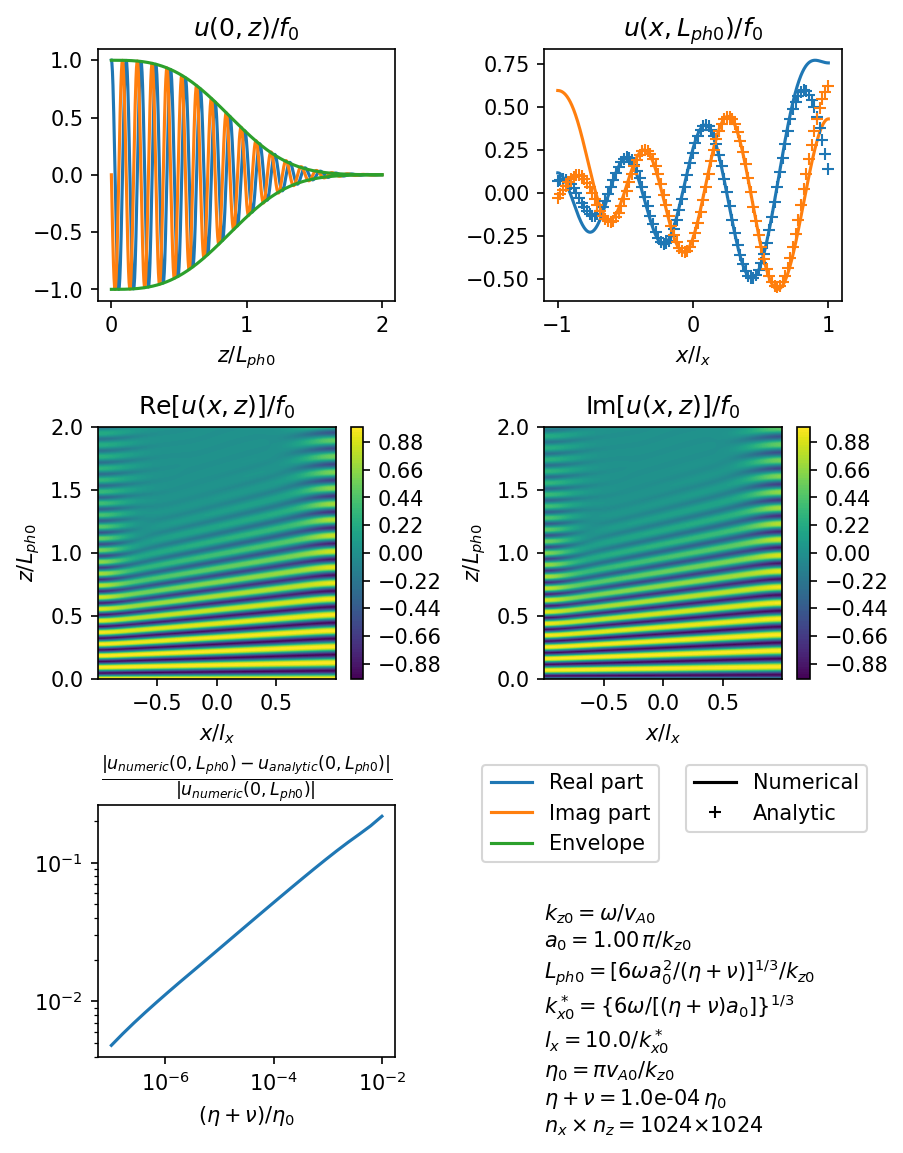
\includegraphics[width=\textwidth,height=0.9\textheight,keepaspectratio]{figures/chapter03/phase_mixing_open_loop.png}
    \vspace{-10pt}
    \caption{This figure shows plots of the velocity perturbation of phase-mixed Alfv\'en waves in an open loop. The top-left shows a plot along $z$ at $x=0$, where the green curve shows the envelope which we calculated using Equation \eqref{eq:velocity_envelope}. The top-right plot shows the analytic and numerical solutions along $x$ at $z=L_{ph0}$. The middle-row shows contour plots of the real and imaginary parts. The bottom-left plots the relative error between the analytic and numerical solutions at $x=0$, $z=L_{ph0}$ as a function of $\eta+\nu$. In the bottom-right, we show some of the parameters we used. The code used to make this figure is available on GitHub in the following directory:\newline
    \href{https://github.com/aleksyprok/apkp_thesis/blob/main/Python/Chapter3/open_loop.py}{$\rightarrow$ Python/Chapter3/open\_loop.py}}
    \vspace{-20pt}
    \label{fig:phase_mxing_open_loop}
\end{figure}

Our goal now is to check that that the numerical solution agrees with the analytic solution. We test this via a graphical approach. In Figure \ref{fig:phase_mxing_open_loop} we plot the velocity perturbation $u$. The top-left shows the velocity along $z$ at $x=0$. The blue and orange curves show the real and imaginary parts, respectively. The green curve shows the envelope, $u_{env}$ which is given by
\begin{equation}
    \label{eq:velocity_envelope}
    u_{env\pm}(x,z) = \pm f_0\exp[-(z/L_{ph})^3],
\end{equation}
which comes from Equation \eqref{eq:leading_order_phase_mixed_soln}. It shows that at $x=0$, to a good approximation, the wave decays with our predicted slope, given by Equation \eqref{eq:leading_order_phase_mixed_soln}. The top-right plot shows the velocity along $x$ at $z=L_{ph0}$, where we show the equation for $L_{ph0}$ in the bottom-right of the figure. The solid line gives the numerical solution and the $+$ symbols give the analytic solution, given by Equation \eqref{eq:leading_order_phase_mixed_soln}. It shows that close to $x=0$, the analytic and numerical solutions show good agreement. However, close to the boundaries, the agreement is poor, and this is because we impose Neumann boundary conditions, see Equation \eqref{eq:neumann_bcs_chap_3}. Our analytic solution works well for open boundary conditions in $x$. However, these are difficult to implement numerically. The middle-row shows contour plots of the real and imaginary parts of the velocity as a function of $x$ and $z$. Finally, the bottom-left shows the relative error between the numerical and analytic solutions at $x=0$ and $z=L_{ph0}$ as a function of $\eta+\nu$. It shows that as we decrease $\eta+\nu$ the error reduces, despite $L_{ph0}$ increasing. In the bottom-right, we show some of the parameters we use, including the grid resolution $n_x\times n_z$.

\section{Closed loop}
\label{sec:chap_3_closed_loop}

In this section we aim to solve Equation \eqref{eq:method_of_lines_eqn_u} for a closed loop, where we impose $u=0$ at the top boundary, i.e.,
\begin{equation}
    u(x,L_z)=0,
\end{equation}
where the domain is given by $z\in[0,L_z]=[0,2l_z]$.

\subsection{Analytic solution}

Using a method of images approach, like that used in Section \ref{sec:closed_loop_sinusoidal_solution}, as well as Equation \eqref{eq:leading_order_phase_mixed_soln}, we calculate the steady-state solution to be
\begin{equation}
    \label{eq:chap_3_closed_loop_phase_mix_soln_u}
    \begin{aligned}
    u(x,z) &= f_0\sum_{k=0}^\infty (-1)^k\exp\qty[-ik_z(x)z_k]\exp[-(z_k / L_{ph})^3] \\
    &= f_0A_\infty(x,z)
    \end{aligned}
\end{equation}
where
\begin{equation}
    z_k = (-1)^k (z-l_z) + (2k+1)l_z,
\end{equation}
and
\begin{equation}
    A_\infty(x,z) = \sum_{k=0}^\infty (-1)^k \exp(-ik_z z_k)\exp[-(z_k / L_{ph})^3].
\end{equation}
Similarly, we calculate the magnetic field to be given by
\begin{equation}
    \label{eq:chap_3_closed_loop_phase_mix_soln_b}
    \begin{aligned}
    b(x,z) &= -B_0\frac{f_0}{v_A}\sum_{k=0}^\infty \exp\qty[-k_z(x)z_k]\exp[-(z_k / L_{ph})^3] \\
    &= -B_0\frac{f_0}{v_A}B_\infty(x,z)
    \end{aligned}
\end{equation}
where
\begin{equation}
    B_\infty(x,z) = \sum_{k=0}^\infty \exp(-ik_z z_k)\exp[-(z_k / L_{ph})^3].
\end{equation}
We are not aware of any method to simplify the summations given by $A_\infty$ and $B_\infty$ further, however, we can approximate them numerically by truncating the series after $N_a$ terms and then calculating the resulting summation numerically, provided $N_a\gg 1$.

\subsection{Numerical solution}

Our goal now is to verify Equations \eqref{eq:chap_3_closed_loop_phase_mix_soln_u} numerically. 
We will convert Equation \eqref{eq:method_of_lines_eqn_u} into a set of ODEs, using the same approach used in Section \ref{sec:chap_2_driven_harmonic_oscillator}. Let
\begin{equation}
    u(x,z) = y(x,z) + f_0\frac{L_z - z}{L_z},
\end{equation}
hence, the boundary conditions for $y$ are
\begin{equation}
    y(x,0)=y(x,L_z)=0.
\end{equation}
We can write Equation \eqref{eq:method_of_lines_eqn_u} as
\[
-i\omega(\eta+\nu)\pdv[2]{y}{x}=\omega^2 y + v_A^2 \pdv[2]{y}{z} + \omega^2f_0\frac{L_z - z}{L_z}.
\]
Note that the we can write the end term as the following Fourier series
\[\omega^2f_0\frac{L_z - z}{L_z} = 2\omega^2f_0\sum_{n=1}^\infty\frac{\sin(k_{zn}z)}{n\pi},\]
where
\begin{equation}
    k_{zn} = \frac{n\pi}{L_z}.
\end{equation}
Let
\begin{equation}
    \label{eq:chap_3_closed_loop_yn}
    y(x,z) = \sum_{n=1}^\infty y_n(x)\sin(k_{zn} z).
\end{equation}
Therefore, each $y_n$ satisfies
\begin{equation}
    \dv[2]{y_n}{x}=i\frac{\omega^2 - v_A^2(x)k_{zn}^2}{\omega(\eta+\nu)}y_n + \frac{2i\omega f_0}{n\pi(\eta+\nu)}.
\end{equation}
We solve this set of ODEs using \texttt{solve\_bvp} in \citet{SciPy2020}. We use the same Alfv\'en speed profile as the last section, namely Equation \eqref{eq:background_vA_chap_3}. We choose the driver frequency, $\omega$, to be given by
 \begin{equation}
     \omega = \frac{\pi v_{A0}}{L_z},
 \end{equation}
 this ensures the driving frequency is equal to the fundamental frequency of the loop at $x=0$.
 Note that we approximate Equation \eqref{eq:chap_3_closed_loop_yn} by truncating the series after $N_h$ terms. We find that the error is small because the solution associated with the fundamental harmonic dominates due to the resonance being excited.
 
\begin{figure}
    \centering
    \vspace{-20pt}
    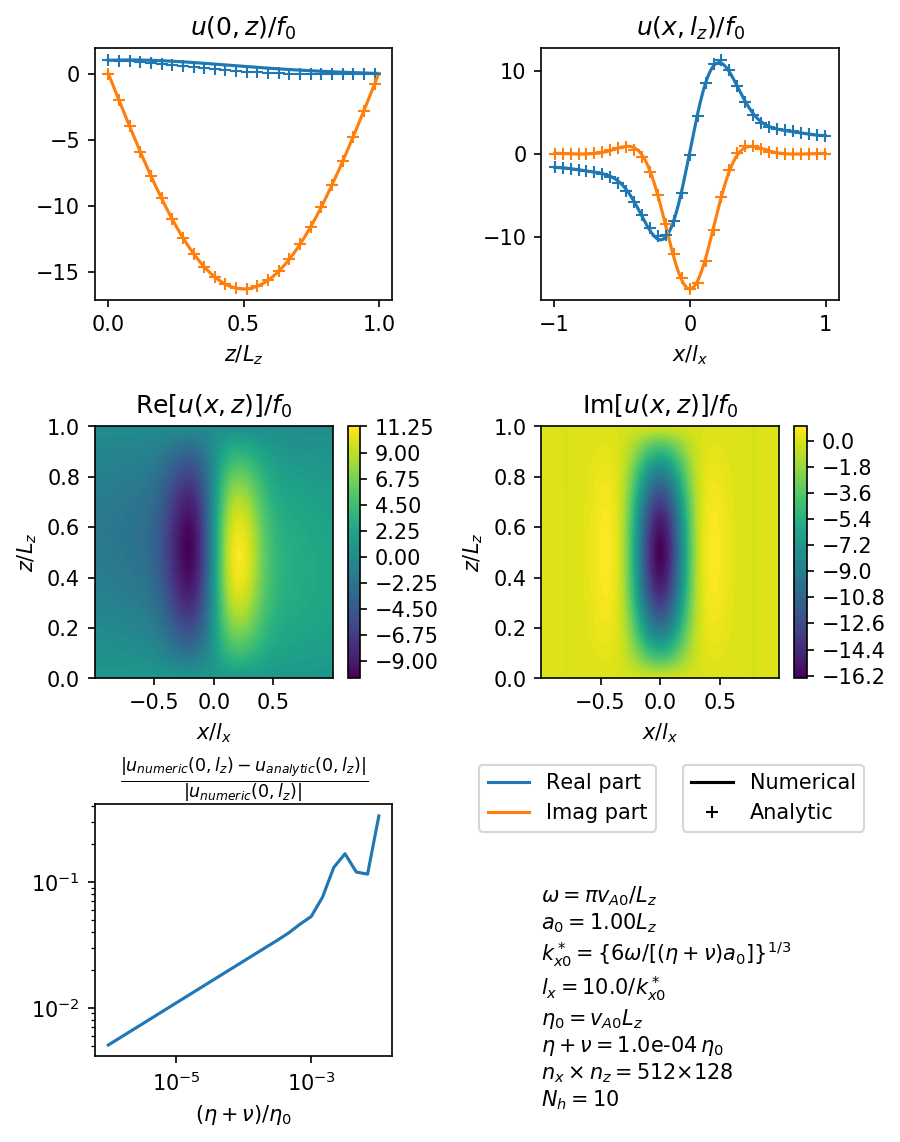
\includegraphics[width=\textwidth,height=0.85\textheight,keepaspectratio]{figures/chapter03/phase_mixing_closed_loop.png}
    \vspace{-10pt}
    \caption{This figure shows plots of the velocity perturbation of phase-mixed Alfv\'en waves in a closed loop. The top-left shows a plot along $z$ at $x=0$. The top-right plot shows the analytic and numerical solutions along $x$ at $z=l_z$. The middle-row shows contour plots of the real and imaginary parts. The bottom-left plots the relative error between the analytic and numerical solutions at $x=0$, $z=l_z$ as a function of $\eta+\nu$. The code used to make this figure is available on GitHub in the following directory:\newline
    \href{https://github.com/aleksyprok/apkp_thesis/blob/main/Python/Chapter3/closed_loop.py}{$\rightarrow$ Python/Chapter3/closed\_loop.py}}
    \label{fig:phase_mixing_closed_loop}
    \vspace{-30pt}
\end{figure}
 
We can now verify Equations \eqref{eq:chap_3_closed_loop_phase_mix_soln_u} via a graphical approach. In Figure \ref{fig:phase_mixing_closed_loop} we plot the velocity perturbation, $u$. The top-left shows the velocity along $z$ at $x=0$. The blue and orange curves show the real and imaginary parts, respectively, see legend in bottom-right of the figure. It shows that the fundamental harmonic dominates the solution because we drive at the field line's fundamental frequency at $x=0$. The top-right plot shows the velocity along $x$ at $z=l_z$, i.e. the middle of the loop. The solid line gives the numerical solution and the $+$ symbols give the analytic solution, given by Equation \eqref{eq:leading_order_phase_mixed_soln}. The imaginary part shows a vertical velocity shear, giving rise to the Kelvin-Helmholtz instability \citep{Heyvaerts1983}. The middle-row shows contour plots of the real and imaginary parts of the velocity as a function of $x$ and $z$. Finally, the bottom-left shows the relative error between the numerical and analytic solutions at $x=0$ and $z=L_{ph0}$ as a function of $\eta+\nu$. It shows that as we decrease $\eta+\nu$, the error reduces.
 
\subsection{Heating rate}
\label{sec:chap_3_closed_loop_heating_rate}
 
In this section, we study the heating rate per unit of wave energy, $\gamma$. Using Equation \eqref{eq:poynting_flux_chap_2} we know that the time-averaged Poynting flux in the $z$-direction, $\langle S_z \rangle$, is given by
\begin{equation}
    \begin{aligned}
    \langle S_z \rangle &= -\frac{B_0}{4\mu}(u\bar{b} + \bar{u}b) \\
    &= \frac{B_0^2f_0^2}{2\mu v_A}\Re(A_\infty\bar{B}_\infty)
    \end{aligned}
\end{equation}
At steady-state, the rate of change of energy in the loop is equal to the loop's heating rate. Therefore, the heating rate is given by the Poynting flux at $z=0$ as the Poynting flux at $z=L_z$ is zero. The time-averaged steady-state wave energy density, $\langle e_\infty \rangle$, is given by
\begin{equation}
    \begin{aligned}
    \langle e_\infty \rangle &= \frac{\rho |u|^2}{4} + \frac{|b|^2}{4\mu} \\
    &= \frac{B_0^2f_0^2}{4\mu v_A^2}(|A_\infty|^2 + |B_\infty|^2).
    \end{aligned}
\end{equation}
Therefore, the heating rate per unit of wave energy, $\gamma$, is given by
\begin{equation}
    \label{eq:gamma_exact_closed_loop}
    \begin{aligned}
    \gamma(x) &= \frac{\langle S_z \rangle|_{z=0}}{\int_{0}^{L_z}\langle e_\infty \rangle dz} \\
    &=2v_A\frac{\Re(A_\infty \bar{B}_\infty)|_{z=0}}{\int_{0}^{L_z}|A_\infty|^2 + |B_\infty|^2dz}.
    \end{aligned}
\end{equation}

Equation \eqref{eq:gamma_exact_closed_loop}, is quite obscure, it is difficult to see how $\gamma$ changes with parameters such as $\omega$ or $\eta+\nu$. Our goal now is to calculate an approximation to Equation \eqref{eq:gamma_exact_closed_loop} which has a more convenient form. Let
\begin{equation}
    B_\infty^*(x,z) = \sum_{k=0}^\infty \exp[-(ik_z+L_{ph}^{-1})z_k]
\end{equation}
where $B_\infty^*$ is nearly the same as $B_\infty$ except the cubic exponential has been replaced with a linear exponential. We postulate that $B_\infty^*\approx B_\infty$ at $x$ provided $k_z(x)L_z=n\pi$ ($n\in\mathds{Z}$). In other words, provided the field line at $x$ is a resonant field line. Note that the form of $B_\infty^*$ is more convenient because we can evaluate the summation using the geometric series formula. We can write $B_\infty^*$ as
\[\begin{aligned}
B_\infty^*(x,z) &= \exp[-(ik_z + L_{ph}^{-1})z]\frac{1}{2}\sum_{k=0}^\infty(1 + (-1)^k) \exp[-(ik_z + L_{ph}^{-1})L_z]^k \\
&+\exp[-(ik_z + L_{ph}^{-1})(L_z-z)]\frac{1}{2}\sum_{k=0}^\infty(1 - (-1)^k) \exp[-(ik_z + L_{ph}^{-1})L_z]^k \\
&=\frac{\exp[-(ik_z + L_{ph}^{-1})z] + r\exp[-(ik_z + L_{ph}^{-1})(L_z - z)]}{1-r^2} \\
&=\frac{\exp[-(ik_z + L_{ph}^{-1})z] + r^2\exp[(ik_z + L_{ph}^{-1})z]}{1-r^2}, \\
\end{aligned}\]
where
\begin{equation}
    r = \exp[-(ik_z+L_{ph}^{-1})L_z].
\end{equation}
If we assume $L_z/L_{ph} \ll 1$ then we can approximate 
\[r = \exp[-ik_zL_z] (1 - L_z / L_{ph} + O[(L_z/L_{ph})^2]).\]
If $k_zL_z = n\pi$ then
\[r^2 = 1 - 2L_z / L_{ph} +  O[(L_z/L_{ph})^2].\]
Hence, if $k_zL_z=n\pi$ then we can approximate $B_\infty^*$ as
\[B_\infty^*(x,0)=\frac{L_{ph}}{L_z} + O[L_z/L_{ph}]).\]
We assume that the energy, $\langle e_\infty \rangle$ is approximately uniformly distributed along $z$, therefore,
\[\begin{aligned}
\int_{0}^{L_z}(|A_\infty|^2 + |B_\infty|^2) dz &\approx |B_\infty^*(x,0)|^2 L_z \\
&= \frac{L_{ph}^2}{L_z} +  O[L_z/L_{ph}]).
\end{aligned}\]
To satisfy the boundary condition, Equation \eqref{eq:driver_chap_3} we know that
\[A_\infty(x,0) = 1.\]
Therefore, the heating rate per unit of wave energy, $\gamma$, is approximated by
\begin{equation}
    \label{eq:gamma_approx_closed_loop}
    \gamma(x) \approx \frac{2 v_A}{L_{ph}}=\omega\qty[\frac{4(\eta+\nu)}{3\omega a^2}]^{1/3},
\end{equation}
provided $k_z(x)L_z = n\pi$.

\begin{figure}
    \vspace{-20pt}
    \centering
    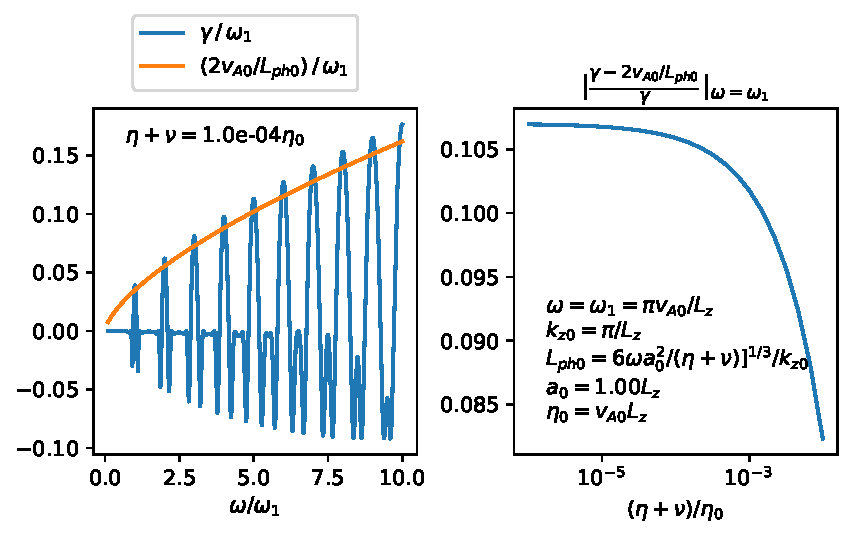
\includegraphics[width=\textwidth,height=0.85\textheight,keepaspectratio]{figures/chapter03/closed_loop_gamma.pdf}
    \vspace{-30pt}
    \caption{This figure shows plots of the heating rate per unit of wave energy, $\gamma$. The left-hand side shows $\gamma$ as a function of frequency. The blue and orange curves were calculated using Equations \eqref{eq:gamma_exact_closed_loop} and \eqref{eq:gamma_approx_closed_loop} respectively. The right-hand side shows the relative error between these two equations as a function of $(\eta+\nu)$. The code used to make this figure is available on GitHub in the following directory:\newline
    \href{https://github.com/aleksyprok/apkp_thesis/blob/main/Python/Chapter3/closed_loop_gamma.py}{$\rightarrow$ Python/Chapter3/closed\_loop\_gamma.py}}
    \label{fig:closed_loop_gamma}
    \vspace{-10pt}
\end{figure}

Our goal now is to verify that Equation \eqref{eq:gamma_approx_closed_loop} provides an approximation for Equation \eqref{eq:gamma_exact_closed_loop} on resonant field lines. Also, we aim to calculate $\gamma$ for the non-resonant field lines. To do this, we take a graphical approach. In Figure \ref{fig:closed_loop_gamma} we present $\gamma$. The blue and orange curves on the left-hand side show $\gamma$ as a function of $\omega$ and were calculated using Equations \eqref{eq:gamma_exact_closed_loop} and \eqref{eq:gamma_approx_closed_loop} respectively. The blue curve shows that $\gamma$ is largest at the resonant frequencies and is significantly smaller away from the resonance and can even be negative. The solution can be negative, and this is because we approximate $\gamma$ here using the Poynting flux instead of the heating rate. Therefore the energy injected into a field line at $z=0$ can be transferred to neighbouring field lines due to diffusion. At first, it may seem surprising that $\gamma$ is so small at non-resonant frequencies because the wave energy, which appears on the denominator of Equation \eqref{eq:gamma_exact_closed_loop}, decreases as the frequency moves away from the resonant frequencies. However, the numerator decreases to a greater degree as the frequency shifts away from the resonant frequencies. Typically, waves need to propagate within the loop for a long time before the length-scales in $x$ become short enough for significant heating to occur. At non-resonant frequencies, waves cannot phase-mix to short enough length-scales before they are eliminated due to destructive interference. Note that the timescale for waves to be eliminated is characterised by the beating time, which we studied in Section \ref{sec:case_where_omega_approx_omega_n}. Comparing the blue and orange curves, we see that Equation \eqref{eq:gamma_approx_closed_loop} provides an approximation for Equation \eqref{eq:gamma_exact_closed_loop} at the resonant frequencies. The right-hand side presents the relative error between the two equations at $\omega=\omega_1$ and as a function of $\eta+\nu$. We see that the relative error remains within about 10\%.

\subsection{Multiple harmonics}
\label{sec:chap_3_closed_loop_multiple_harmonics}

We showed in Section \ref{sec:mhd_waves_power_spectrum} that velocity fluctuations oscillate at a broad range of frequencies. In this section, we aim to calculate the heating rate per unit of wave energy, $\gamma$, for the case where the driver excites a broad range of frequencies. In Section \ref{sec:closed_loop_random_driver}, we showed that the power spectrum in a closed loop with a broadband driver will on average have peaks at the resonant frequencies. \citet{Wright1995} have also observed this. Therefore, for simplicity, our driver will only excite the resonant frequencies.

Let the bottom boundary condition be given by
\begin{equation}
    \label{eq:driver_multiple_harmonics}
    \begin{aligned}
    u(x,0,t) &= f_{driv}(t)\\
    &=f_0 \sum_{n=-N}^N C_n \exp(i\omega_n t),
    \end{aligned}
\end{equation}
where
\begin{gather}
    C_n = \begin{dcases}
    0, & n=0, \\
    \frac{\sqrt{L_z} n^{-\alpha / 2}\exp(i\varphi_n)}{\sqrt{\int_0^{L_z} |A_{\infty,n}|^2 + |B_{\infty,n}|^2 dz}}, & n > 0, \\
   \bar{C}_{|n|}, & n < 0,
    \end{dcases} \\
    A_{\infty,n} = \sum_{k=0}^\infty(-1)^k\exp(-ik_{z,n}z_k)\exp[-(z_k / L_{ph,n})], \\
    B_{\infty,n} = \sum_{k=0}^\infty \exp(-ik_{z,n}z_k)\exp[-(z_k / L_{ph,n})], \\
    \omega_n = n\frac{\pi v_{A0}}{L_z}, \\
    k_{z,n} = \frac{\omega_n}{v_{A0}}, \\
    L_{ph,n} = \qty[\frac{6\omega_n a^2}{\eta+\nu}]^{1/3}\frac{1}{k_{z,n}}.
\end{gather}
Note that $\alpha$ controls the slope of the power spectrum, $\varphi_n\in\mathds{R}$ gives an arbitrary phase, $\bar{C}_{|n|}$ denotes the complex conjugate and ensures the driver is real and $N$ controls the number of harmonics which are excited. From Equations \eqref{eq:chap_3_closed_loop_phase_mix_soln_u} and \eqref{eq:chap_3_closed_loop_phase_mix_soln_b} we know that the steady-state solutions are given by
\begin{gather}
    u(x,z,t) = f_0\sum_{n=-N}^NA_{\infty,n}C_n\exp(i\omega_n t), \\
    b(x,z,t) = -B_0\frac{f_0}{v_A}\sum_{n=-N}^NB_{\infty,n}C_n\exp(i\omega_n t).
\end{gather}

By Parsvel's theorem, the time-averaged energy is given by
\begin{equation}
    \begin{aligned}
    \langle e_\infty \rangle &=\frac{1}{P}\int_0^{P}\frac{\rho |u|^2}{4} + \frac{|b|^2}{4\mu}dt
\\&=\frac{B_0^2f_0^2}{4\mu v_A^2}\sum_{n=-N}^N |A_{\infty,n} C_n|^2 + |B_{\infty,n} C_n|^2,
    \end{aligned}
\end{equation}
where
\begin{equation}
    P = \frac{2L_z}{v_{A0}}.
\end{equation}
Therefore, the energy of the whole loop, $\langle E_\infty \rangle$, is given by
\begin{equation}
    \begin{aligned}
    \langle E_\infty \rangle &= \frac{B_0^2f_0^2}{4\mu v_A^2}\sum_{n=-N}^N|C_n|^2\int_0^{L_z}|A_{\infty,n}|^2+|B_{\infty,n}|^2 dz \\
    &= \frac{B_0^2f_0^2}{2\mu v_A^2}L_z\sum_{n=1}^Nn^{-\alpha}.
    \end{aligned}
\end{equation}
The above equations shows that our driver, Equation \eqref{eq:driver_multiple_harmonics}, ensures that the energy of the loop has a power spectrum with slope $\omega_n^{-\alpha}$.

Using Parseval's theorem, the average Poynting flux is given by
\begin{equation}
    \begin{aligned}
    \langle S_z \rangle &= \frac{B_0^2f_0^2}{2\mu v_A}\sum_{n=-N}^N|C_n|^2\Re(A_{\infty,n}\bar{B}_{\infty,n}) \\
    &= \frac{B_0^2f_0^2}{\mu v_A}L_z\sum_{n=1}^Nn^{-\alpha}\frac{\Re(A_{\infty,n}\bar{B}_{\infty,n})}{\int_0^{L_z}|A_{\infty,n}|^2+|B_{\infty,n}|^2dz}.
    \end{aligned}
\end{equation}
Therefore, the heating rate per unit of wave energy, $\gamma$, is given by
\begin{equation}
    \label{eq:gamma_multiple_harmonics_exact}
    \begin{aligned}
    \gamma &= \frac{\langle S_z\rangle|_{z=0}}{\langle E_{\infty} \rangle} \\
    &=\frac{\sum_{n=1}^Nn^{-\alpha}\gamma_n}{\sum_{n=1}^Nn^{-\alpha}},
    \end{aligned}
\end{equation}
where
\begin{equation}
    \gamma_n = 2v_A\frac{\Re(A_{\infty,n}\bar{B}_{\infty,n})|_{z=0}}{\int_0^{L_z}|A_{\infty,n}|^2+|B_{\infty,n}|^2dz}.
\end{equation}
Hence, $\gamma$ takes the form of a weighted average of the set $\{\gamma_n\}$ with weights $n^{-\alpha}$.

Our goal now is to approximate Equation \eqref{eq:gamma_multiple_harmonics_exact} in a more convenient form. We approximate $\gamma_n$ by using Equation \eqref{eq:gamma_approx_closed_loop} to give
\begin{equation}
    \begin{aligned}
    \gamma_n &\approx \omega_n\qty[\frac{4(\eta+\nu)}{3\omega_na^2}]^{1/3} \\
    &= \omega_1\qty[\frac{4(\eta+\nu)}{3\omega_1a^2}]^{1/3}n^{2/3}.
    \end{aligned}
\end{equation}
Hence, Equation \eqref{eq:gamma_multiple_harmonics_exact} can be approximated as
\begin{equation}
    \label{eq:gamma_multiple_harmonics_approx}
    \begin{aligned}
    \gamma &\approx \gamma_1\frac{\sum_{n=1}^Nn^{2/3-\alpha}}{\sum_{n=1}^Nn^{-\alpha}} \\
    &= \gamma_1\frac{H_N^{(\alpha-2/3)}}{H_N^{(\alpha)}},
    \end{aligned}
\end{equation}
where $H_N^{(p)}$ denotes the generalised harmonic number of order $p$ of $n$.
Note that
\begin{equation}
\label{eq:generalised_harmonic_number_approx}
H_N^{(p)}=
    \begin{dcases}
    \ln(N) + \gamma_{EM} + O(1/N), & p=1 \\
    N^{-p}\qty[\frac{N}{1-p}+\frac{1}{2}+O(1/N)] + \zeta(p), & p\ne 1 \\
    \end{dcases}
\end{equation}
where $\zeta(p)$ denotes the Riemann zeta function (see right-side of Figure \ref{fig:multiple_harmonics}) and $\gamma_{EM}$ is the Euler-Mascheroni constant. Hence, 
if $\alpha=0$, then to leading order
\begin{equation}
    \label{eq:gamma_alpha=0}
    \gamma \approx \gamma_1\frac{3N^{2/3}}{5} + O(N^{-1/3}),
\end{equation}
if $\alpha = 1$, then to leading order
\begin{equation}
    \label{eq:gamma_approx_alpha=1}
    \gamma \approx \gamma_1\frac{3N^{2/3}/2+\zeta(1/3) + O(N^{-1/3})}{\ln(N)+\gamma_{EM}+O(1/N)},
\end{equation}
if $\alpha=5/3$, then to leading order
\begin{equation}
    \label{eq:gamma_alpha=5/3}
    \gamma \approx \gamma_1\frac{\ln(N) + \gamma_{EM} + O(1/N)}{\zeta(5/3)+O(N^{-2/3})}.
\end{equation}

Our goal now is to check that $\gamma$, given by Equation \eqref{eq:gamma_multiple_harmonics_exact}, can be approximated with Equation \eqref{eq:gamma_multiple_harmonics_approx} with $H_N^{(p)}$ approximated by Equation \eqref{eq:generalised_harmonic_number_approx}. We test this using a graphical approach. On the left-side of Figure \ref{fig:multiple_harmonics} we plot the heating rate per unit of wave energy, $\gamma$, as a function of the number of excited harmonics, $N$, for different power spectra slopes, $\alpha$. The exact solution (solid line) was calculated using Equation \eqref{eq:gamma_multiple_harmonics_approx}. The approximate solution (`+' symbols), was calculated using \eqref{eq:gamma_multiple_harmonics_exact} with with $H_N^{(p)}$ approximated by Equation \eqref{eq:generalised_harmonic_number_approx}. Note that to account for the error associated with approximating $\gamma$ with Equation \eqref{eq:gamma_approx_closed_loop} we multiply our approximation by a factor 1.1. This factor comes from the fact that we noted an error of about 10\% in Figure \ref{fig:closed_loop_gamma}.
We plot for the case where $\alpha=0$ (blue), $1$ (orange), and $5/3$ (green), these can be approximated with Equations \eqref{eq:gamma_alpha=0}-\eqref{eq:gamma_alpha=5/3} respectively. The plots suggest that our approximation is indeed accurate for $N\gg1$. Note that if the power spectra are steep, $\alpha=5/3$ say, then $\gamma$ is weakly dependent on the number of harmonics. If the power spectra are flatter, $\alpha=0$, then $\gamma$ is highly dependent on the number of excited harmonics.

\begin{figure}
    \centering
    \vspace{-20pt}
    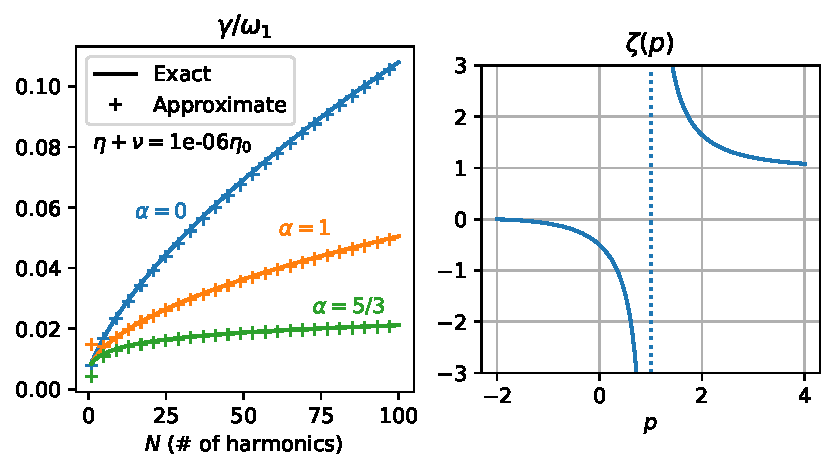
\includegraphics[width=\textwidth,height=0.85\textheight,keepaspectratio]{figures/chapter03/multiple_harmonics.pdf}
    \vspace{-30pt}
    \caption{This figure shows line plots of the heating rate per unit of wave energy as a function of the number of excited harmonics, $N$, on the left. 
    % The exact solution was calculated using Equation \eqref{eq:gamma_multiple_harmonics_approx}  and the approximate solution was calculated using \eqref{eq:gamma_multiple_harmonics_exact} with with $H_N^{(p)}$ approximated by Equation \eqref{eq:generalised_harmonic_number_approx}. 
    The right-side shows the Riemann zeta function along the real axis where the discontinuity at $p=1$ is denoted with a dotted line. The code used to make this figure is available on GitHub in the following directory:\newline
    \href{https://github.com/aleksyprok/apkp_thesis/blob/main/Python/Chapter3/multiple_harmonics.py}{$\rightarrow$ Python/Chapter3/multiple\_harmonics.py}}
    \vspace{-20pt}
    \label{fig:multiple_harmonics}
\end{figure}

Figure \ref{fig:multiple_harmonics} uses a range of $\alpha$ values including $5/3$ as this is one the values predicted from MHD turbulence theory \citep{Bruno2013}. \citet{Morton2016} provides observations of the power spectra of velocity fluctuations in the quiet sun, the active regions, and the coronal holes (see Figure \ref{fig:power_spectrum_morton}). These latter authors find that the slope varies from $\alpha = 1$ to $\alpha = 1.53$ for higher frequencies, although they are only able to measure up to frequencies of around $10^{-2}\si{.Hz}$. \citet{Podesta2007} measure the power spectra in the solar wind and can measure up to $10^{-1}\si{.Hz}$ and find the slope to be between $\alpha = 1.5$ $\alpha = 5/3$.

\section{Leaky loop}
\label{sec:chap_3_leaky_loop}

In Section \ref{sec:leaky_loop_reflection_coefficent}, we showed that waves can leak out of the corona. In this section, we aim to study phase-mixed Alfv\'en waves in a leaky loop and calculate the effects of leakage on the value of $\gamma$. We use similar boundary conditions to those used in Section \ref{sec:leaky_loop_general_solution}, namely, 
\begin{equation}
    \tag{\ref{eq:bcs_elsasser}}
    \begin{aligned}
    \mathcal{Z}^{-}(x,0,t) &= 2f_{driv}(x,t) - R\mathcal{Z}^+(x,0,t) \\
    \mathcal{Z}^{+}(x,L_z,t) &= -R\mathcal{Z}^-(x,L_z,t),
    \end{aligned}
\end{equation}
where $R$ gives the reflection coefficient, which we approximate in Section \ref{sec:leaky_loop_reflection_coefficent}. These boundary conditions ensure that each time a wave reaches a boundary a fraction $R$ of the wave is reflected and a fraction $1-R$ leaks out of the loop.

Our first goal is to calculate the timescale at which waves decay due to leakage. We will compare this with the resisitive timescale to estimate the parameter space in which leakage plays a significant role in the decay of waves compared with resistive effects. Consider an ideal loop. The time taken for a wave to travel from $z=0$ to $z=L_z$ (and vice versa) is the Alfv\'en travel time, $\tau_A$, given by
\begin{equation}
    \label{eq:chap_3_alfven_travel_time}
    \tau_A = \frac{L_z}{v_A}.
\end{equation}
Therefore each time $\tau_A$ time units have elapsed the wave amplitude decreases by $R$. Thus, the wave amplitude, $u_0$, goes as
\begin{equation}
    \begin{aligned}
    u_0 &\propto R^{\lfloor t / t_{A} \rfloor} \\
    &= \exp\qty(\left\lfloor\frac{t}{t_A}\right\rfloor\ln R) \\
    &\approx \exp\qty(-\frac{|\ln R|}{t_A}t).
    \end{aligned}
\end{equation}
Hence, the leakage timescale, $\tau_{leakage}$, is given by,
\begin{equation}
    \tau_{leakage} = \frac{L_z}{v_A |\ln R|}.
\end{equation}
Each time a wave propagates a distance, $L_{ph}$, the wave decays by a factor $\exp(1)$ due to resistive effects. Therefore, the resistive timescale is given by 
\begin{equation}
\begin{aligned}
    \tau_{resistive} &= \frac{L_{ph}}{v_A} \\
    &= \qty[\frac{6\omega^2a^2}{\eta+\nu}]^{1/3}\frac{1}{\omega}.
\end{aligned}
\end{equation}
If $\tau_{resistive}\ll\tau_{leakage}$ then we expect leakage to play a negligible role and the solution to be well approximated by our calculation in Section \ref{sec:chap_3_closed_loop}. If $\tau_{resistive}\ll\tau_{leakage}$ then we expect resistivity and viscosity to play negligible role in determining the shape of the solution, however, any heating which occurs will still be Ohmic and viscous. To get an idea of the parameter space in which leakage plays an important we plot $\tau_{resistive}$ and $\tau_{leakage}$ on the left-hand side of Figure \ref{fig:chap_3_leaky_loop} as a function of $f$ in $\si{Hz}$. The plot shows that the leakage timescale is smaller than the resistive timescale for this parameter space. We show our choice of parameters in the figure, e.g. we assume a background Alfv\'en speed of $10^6\si{.m.s^{-1}}$, where we chose the parameters to represent typical values in coronal loops.

\begin{figure}
    \vspace{-20pt}
    \centering
    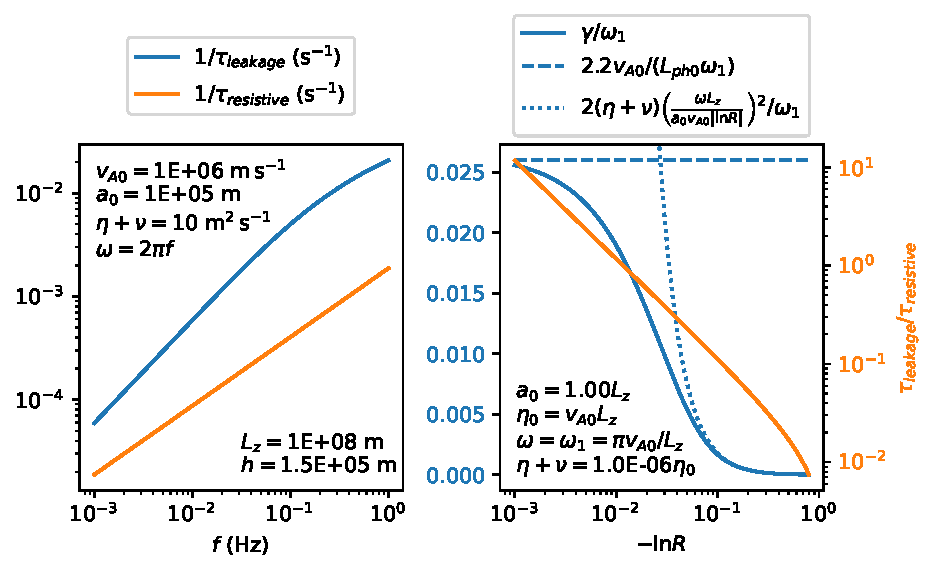
\includegraphics[width=\textwidth,height=0.85\textheight,keepaspectratio]{figures/chapter03/leaky_loop.pdf}
    \vspace{-35pt}
    \caption{This figure shows plots of the leakage timescale, $\tau_{leakage}$, and resistive timescale, $\tau_{resistive}$ on the left as a function of the wave frequency. The right-side shows $\gamma$ in blue and the ratio, $\tau_{leakage}/\tau_{resistive}$, in orange, as a function of the reflection coefficient, R. The code used to make this figure is available on GitHub in the following directory:\newline
    \href{https://github.com/aleksyprok/apkp_thesis/blob/main/Python/Chapter3/leaky_loop.py}{$\rightarrow$ Python/Chapter3/leaky\_loop.py}}
    \label{fig:chap_3_leaky_loop}
    \vspace{-15pt}
\end{figure}

Extending Equations \eqref{eq:chap_3_closed_loop_phase_mix_soln_u} and \eqref{eq:chap_3_closed_loop_phase_mix_soln_b} to include leakage gives
\begin{gather}
\label{eq:chap_3_full_soln_leaky_resistive_u}
\begin{aligned}
    u(x,z) &= f_0\sum_{k=0}^\infty(-1)^kR^k\exp[-ik_z(x)z_k]\exp[-(z_k/L_{ph})^3] \\
    &= f_0A_\infty'(x,z),
\end{aligned}
\\
\begin{aligned}
    b(x,z) &= -B_0\frac{f_0}{v_A}\sum_{k=0}^\infty R^k\exp[-ik_z(x)z_k]\exp[-(z_k/L_{ph})^3] \\
    &= -B_0\frac{f_0}{v_A}B_\infty'(x,z),
\end{aligned}
\end{gather}
where
\begin{gather}
    A_\infty'(x,z) = \sum_{k=0}^\infty(-1)^kR^k\exp[-ik_z(x)z_k]\exp[-(z_k/L_{ph})^3], \\
    B_\infty'(x,z) = \sum_{k=0}^\infty R^k\exp[-ik_z(x)z_k]\exp[-(z_k/L_{ph})^3].
\end{gather}
Introducing leakage means that the Poynting flux at $z=L_z$ is no longer necessarily equal to zero, therefore, the heating rate per unit of wave energy is given by
\begin{equation}
    \label{eq:gamma_exact_leaky_loop}
    \gamma(x) = -2v_A\frac{[\Re(A_\infty'\bar{B}_\infty')]_{z=0}^{z=L_z}}{\int_0^{L_z}|A_\infty'|^2+|B_\infty'|^2dz)}.
\end{equation}

The above equation for $\gamma$ is quite cumbersome because it is difficult to see its dependency on parameters such as $\omega$ or $R$. Our goal now is to calculate an approximate solution for the case where $\tau_{leakage}\ll \tau_{resistive}$. Note that Equation \eqref{eq:gamma_approx_closed_loop} gives an approximate solution for $\tau_{leakage}\gg \tau_{resistive}$. The heating rate per unit of wave energy, $\gamma$, is approximated by
\begin{equation}
    \begin{aligned}
    \gamma &\approx \frac{\frac{1}{2}(\eta+\nu)\int_0^{L_z}\rho (\pdv*{u}{x})^2 + (\pdv*{b}{x})^2/\mu dz}{\frac{1}{2}\int_0^{L_z}\rho u^2 + b^2/\mu dz} \\
    &\approx (\eta+\nu)(k_x^*)^2,
    \end{aligned}
\end{equation}
where $k_x^*$ gives a measure of the wavenumber in the $x$-direction. Substituting $z=v_A t$, we estimate $k_x^*$ in the strong leakage limit as
\begin{equation}
\begin{aligned}
    k_x^* &\approx \frac{\omega}{a}\tau_{leakage} \\
    &=\frac{\omega L_z}{a v_A |\ln R|}.
\end{aligned}
\end{equation}
Therefore,in the strong leakage limit,
\[
    \gamma \propto (\eta + \nu)\qty(\frac{\omega L_z}{a v_A |\ln R|})^2.
\]
Note that the dotted curve in Figure \ref{fig:chap_3_leaky_loop} uses
\begin{equation}
    \label{eq:gamma_approx_leaky_loop}
    \gamma = 2(\eta + \nu)\qty(\frac{\omega L_z}{a v_A |\ln R|})^2.
\end{equation}

We now need to plot $\gamma$, given by Equation \eqref{eq:gamma_exact_leaky_loop}, as a function of $R$, to see how leakage affects $\gamma$ and to check the accuracy of Equation \eqref{eq:gamma_approx_leaky_loop}. The solid blue curve on the right-hand side of Figure \ref{fig:chap_3_leaky_loop} shows $\gamma$ as a function of the reflection coefficient $-\ln R$. The plot shows that increasing the leakage (decreasing $R$) causes $\gamma$ to decrease. This is because the leakage reduces the development of short length-scales as waves leak out of the loop before they can phase-mix to the same length-scales that closed-loop waves can reach. The Figure shows that in the limit $\tau_{leakage} / \tau_{resistive} \ll 1$, then $\gamma$ can be approximated with Equation \eqref{eq:gamma_approx_leaky_loop}, where the ratio $\tau_{leakage} / \tau_{resistive}$, is plotted in orange and the approximation is plotted with a dotted blue line. In the limit $\tau_{leakage} / \tau_{resistive} \gg 1$ then $\gamma$ can be well approximated by assuming the loop is closed.

\section{Coronal heating discussion}
\label{sec:chap_3_coronal_heating}

In Section \ref{sec:chap_3_introduction} we showed that we require $\gamma\approx10^{-1}\si{.s^{-1}}$, see Equation \eqref{eq:required_gamma}, for phase mixing to play an important role in coronal heating. Our goal now is to use results from Sections \ref{sec:chap_3_closed_loop}-\ref{sec:chap_3_leaky_loop} to estimate an upper bound for a typical value of $\gamma$ in the closed corona using phase-mixing theory. We will first present our estimate. After that, we will discuss some of our simplifications and calculate if they increase or decrease our estimate of $\gamma$.

In Section \ref{sec:chap_3_closed_loop_heating_rate} we showed that if a single harmonic is excited, then $\gamma$ can be well approximated with Equation \eqref{eq:gamma_approx_closed_loop}. Velocity fluctuations in the corona typically oscillate at a superposition of multiple frequencies, with a power spectrum approximated by Figure \ref{fig:power_spectrum_morton}. In Section \ref{sec:chap_3_closed_loop_multiple_harmonics}, we showed if multiple harmonics are excited and have a power spectrum proportional to $f^{-\alpha}$, where $f$ denotes the frequency of the waves, then $\gamma$ is approximated with Equation \eqref{eq:gamma_multiple_harmonics_approx}. Substituting for typical values, with $\alpha=1$, $N=100$, Equation \eqref{eq:gamma_approx_alpha=1} gives
\begin{equation}
    \label{eq:upper_bound_for_gammma}
    \gamma \approx 1.43\times10^{-4} \qty(\frac{\omega_1}{\pi\times10^{-2}\si{.Hz}})^{1/3}\qty(\frac{\eta+\nu}{10\si{.m^2.s^{-1}}})^{1/3}\qty(\frac{1\si{.Mm}}{a})^{2/3}\si{.s^{-1}}.
\end{equation}
Therefore, our upper bound for $\gamma$ is significantly less than the required value of $\gamma$, by approximately three orders of magnitude. This implies that the $\vec{W}^{(1)}$ component of the viscosity tensor, $\vec{\sigma}_{Brag}$, plays a negligible role in coronal heating. This suggests that the direct dissipation of waves due to the steep gradients generated by phase-mixing play an insignificant role in coronal heating. However, phase mixing could still play an important but less direct role in coronal heating. For example, phase mixed Alfv\'en waves are susceptible to the Kelvin-Helmholtz and tearing mode instabilities, leading to a turbulent cascade to smaller scales. This would mean that the dissipation occurs primarily due to gradients parallel to the field or the velocity which are dissipated via the $\vec{W}^{(0)}$ component of the viscosity tensor. Note that $\vec{W}^{(0)}$ is not dependent on the gradients generated through phase-mixing since the $x$-direction is neither parallel to the field or the velocity. In \citet{Hillier2019} they show that the Kelvin-Helmholtz instability can lead to coronal cooling as a result of the fluid mixing together which causes the temperate to become more uniform resulting in the total amount of radiation increases. To derive the above equations, we had to make several simplifications. The rest of this section justifies these simplifications and explains why we chose the values for the above parameters.

Increasing $\alpha$ acts to reduce $\gamma$. For our calculation we took $\alpha=1$, which underestimates the single power-law fit to Figure \ref{fig:power_spectrum_morton}. This helps ensure that our calculation for $\gamma$ is an upper bound. We chose $N=100$ because $100\omega = \pi\si{.Hz}$ which is a higher than the maximum observed wave frequencies. We will also show later, in Equation \eqref{eq:w01}, for high frequencies, phase mixing plays a negligible role in the dissipation of waves compared with the dissipation due to gradients parallel to the background field. The characteristic length of a coronal loop is about $100\si{.Mm}$ \citep{O'Neill2005} with an average Alfv\'en speed of about $1\si{.Mm.s^{-1}}$ \citep{McIntosh2011}. This gives a fundamental angular frequency of $\omega_1=\pi\times10^{-2}\si{.Hz}$. Combining Equations \eqref{eq:braginskii_eta_1} and \eqref{eq:proton_gyrofrequency_times_collision_time} gives
\begin{equation}
    \label{eq:nu_typical_values}
    \nu=\frac{\eta_1}{\rho} = 0.62\,\qty(\frac{10^{-3}\si{.Tesla}}{B_0})^2\qty(\frac{10^6\si{.K}}{T})^{1/2}\qty(\frac{\rho}{10^{-12}\si{.kg.m^{-3}}})\si{.m^2.s^{-1}},
\end{equation}
where the Coulomb logarithm, $\log\Lambda$, has been set equal to $20$. Therefore, Equations \eqref{eq:eta_typical_values} and \eqref{eq:nu_typical_values} show that $\eta+\nu<10\si{.m^2.s^{-1}}$ for the given set of parameters. The parameter with the greatest level of uncertainty associated with it is the length-scale of the Alfv\'en travel times, $a$, given by Equation \eqref{eq:length_scale_alfven_travel_time}. We discuss a suitable value for $a$ in the next paragraph. 

Three factors determine the Alfv\'en travel time of a loop, the length of the loop, the plasma density, and the magnetic field strength. In \citet{Oliver1993}, they calculate the Alfv\'en travel time in a potential coronal arcade with a uniform density profile. The flux function, $A$, is given by
\begin{equation}
    \label{eq:potential_aracde_flux_function}
    A(x,z) = B_0\Lambda_B\cos(\frac{x}{\Lambda_B})\exp(-\frac{z}{\Lambda_B}),
\end{equation}
where $B_0$ gives the field strength at $z=0$, $\Lambda_B$ gives the scale height of the field strength and is also related to the arcade's lateral extent. Note that lines of constant $A$ provide the field lines and the associated magnetic field is given by $\vec{B}=\grad{A}\cross\vec{\hat{y}}$. We plot the field on the left side of Figure \ref{fig:potential_arcade}. In \citet{Oliver1993} they show that the fundamental frequency of this arcade is given by
\begin{equation}
    \omega_1 = \pi\frac{v_{A0}}{2x_0}\cos(\frac{x_0}{\Lambda_B}),
\end{equation}
where $v_{A0}$ gives the Alfv\'en speed at $z=0$ and $x_0$ gives the $x$-coordinate of the field line at $z=0$. Therefore, the length-scale of Alfv\'en travel time variations across the field lines can be approximated with
\begin{equation}
    \begin{aligned}
    a(x_0) &= \abs{\frac{\omega_1}{\dv*{\omega_1}{x_0}}} \\
    &= \frac{x_0\Lambda_B\cos(x_0/\Lambda_B)}{\Lambda_B\cos(x_0/\Lambda_B)+x_0\sin(x_0/\Lambda_B)}.
    \end{aligned}
\end{equation}
Note that $a(x_0)$ is plotted on the right-side of Figure \ref{fig:potential_arcade}. The plot shows that $a = 0$ for $x_0=0$ and $x_0=\pi\Lambda_B/2$.  The magnetic field lines are highly divergent near $x_0=\pi\Lambda_B/2$. It has been shown in for example \citet{Smith2007} that a diverging field can enhance the phase mixing. However, we are interested in an average value for $a$. The average value, $\langle a \rangle$ is given by
\begin{equation}
\begin{aligned}
    \langle a(x_0) \rangle &= \frac{2}{\pi\Lambda_B}\int_0^{\pi\Lambda_B/2}a(x_0)dx_0 \\
    &= \frac{2}{\pi}\ln(\frac{\pi}{2})\Lambda_B \\
    &\approx 2.87\qty(\frac{\Lambda_B}{10\si{.Mm}}) \si{.Mm}.
\end{aligned}
\end{equation}
For $x_0\rightarrow0$, $\omega_1\rightarrow\infty$. Therefore, a resonance near $x_0=0$ must have a very high frequency. Figure \ref{fig:reflection_coefficent} showed that very high frequencies can leak into the chromosphere more easily. This suggests imposing solid boundary conditions may not be appropriate here.
The Alfv\'en travel time is also affected by the density of the plasma. \citet{Klimchuk2015} shows that coronal loops have a characteristic diameter of approximately $1.5\si{.Mm}$. If we assume a density contrast, $\rho_i/\rho_o=2$, \citep{Hood2013,Pascoe2013} where $\rho_i$ gives the density inside a loop and $\rho_o$ gives the density outside a loop then this gives a length-scale $a\approx750\si{.km}$.

\begin{figure}
    \centering
    \vspace{-20pt}
    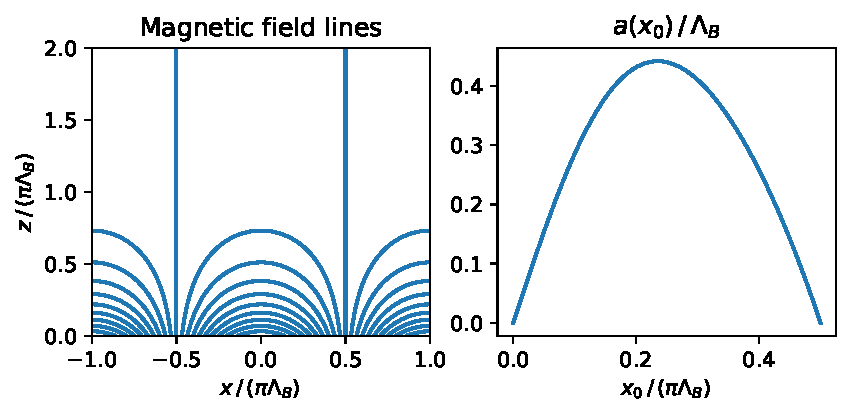
\includegraphics[width=\textwidth,height=0.8\textheight,keepaspectratio]{figures/chapter03/potential_arcade.pdf}
    \vspace{-30pt}
    \caption{This figure's left side shows a plot of the magnetic field lines where the flux function is given by Equation \eqref{eq:potential_aracde_flux_function}. The right side shows plots of $a$ for the field lines as a function of the footpoint coordinate, $x_0$. The code used to make this figure is available on GitHub in the following directory:\newline
    \href{https://github.com/aleksyprok/apkp_thesis/blob/main/Python/Chapter3/potential_arcade.py}{$\rightarrow$ Python/Chapter3/potential\_arcade.py}}
    \vspace{-10pt}
    \label{fig:potential_arcade}
\end{figure}

We modelled the system as linear. This meant the $\vec{W}^{(0)}$ component of the viscosity was neglected. If we assume $\vec{u}=u(x,z,t)\vec{\hat{y}}$ and $\vec{B}=B_0\vec{\hat{z}} + b(x,z,t)\vec{\hat{y}}$ and don't linearise, then
\begin{equation}
    \eta_0\vec{W}^{(0)}:\grad{\vec{u}} = 3\eta_0\epsilon^2\qty(\pdv{u}{z})^2 + O(\epsilon^3),
\end{equation}
where $\epsilon=u/v_A$.
Therefore, the ratio, $w_{0,1}$, between the heating generated by $\vec{W}^{(0)}$ and $\vec{W}^{(1)}$ can be estimated. For simplicity we choose $\eta=0$, hence,
\begin{equation}
\label{eq:w01}
\begin{aligned}
    w_{0,1} &= \frac{\eta_0\vec{W}^{(0)}:\grad{\vec{u}}}{\eta_1\vec{W}^{(1)}:\grad{\vec{u}}} \\
    &\approx 3\epsilon^2\frac{\eta_0}{\eta_1}\qty(\frac{k_z}{k_x^*})^2 \\
    &\approx 4.0471\times10^{-6}\frac{e^{2/3}\mu}{(\ln\Lambda)^{4/3}}\epsilon^2\frac{T^{8/9}\omega^{4/3}}{\rho^{1/3}B_0^{4/3}}a^{2/3} \\
    &\approx 0.59\times10^{-2}\qty(\frac{\epsilon}{10^{-1}})^2\qty(\frac{T}{10^{6}\si{.K}})^{8/9}\qty(\frac{\omega}{\pi\times10^{-2}\si{.Hz}})^{4/3}\\
    &\times\qty(\frac{10^{-12}\si{.kg.m^{-3}}}{\rho})^{1/3}\qty(\frac{10^{-3}\si{.T}}{B_0})^{4/3}\qty(\frac{a}{10^5\si{.m}})^{2/3},
\end{aligned}
\end{equation}
where $k_x^*$ is given by Equation \eqref{eq:phase_mixed_x_length_scale}.

Another consequence of linearising the system is that it causes the Alfv\'en waves to become decoupled from the fast and slow waves. To see this, consider the $y$-component of the ideal momentum equation, Equation \eqref{eq:momentum}, with gravity neglected, $\pdv*{}{y}=0$ and multiplied by $v_y=u$,
\begin{equation}
    \rho\pdv{}{t}\qty(\frac{1}{2}v_y^2)+\rho\vec{v}\vdot\grad\qty(\frac{1}{2}v_y^2)=(\vec{B}\vdot\grad)B_y,
\end{equation}
where $B_y=b$.
Consider the the mass continuity equation, Equation \eqref{eq:mass_continuity}, multiplied by $v_y^2/2$ to give 
\begin{equation}
    \frac{1}{2}v_y^2\pdv{\rho}{t}+\frac{1}{2}v_y^2\div(\rho\vec{v})=0.
\end{equation}
Combining the above equations gives the equation for the evolution of the Alfv\'en wave kinetic energy,
\begin{equation}
    \label{eq:nonlinear_alfven_wave_kinetic_energy}
    \pdv{}{t}\qty(\frac{1}{2}\rho v_y^2) + \div(\frac{1}{2}\rho v_y^2\vec{v})=\frac{1}{\mu}v_y(\vec{B}\vdot\grad)B_y.
\end{equation}
Taking the dot product of Faraday's Law, Equation \eqref{eq:faradays_law}, with $\vec{B}_y/\mu=B_y/\mu\vec{\hat{y}}$, gives
\begin{equation}
    \begin{aligned}
    \pdv{}{t}\qty(\frac{B_y^2}{2\mu})&=-\frac{\vec{B}_y}{\mu}\vdot\curl{\vec{E}} \\
    &=-\div(\frac{\vec{E}\cross\vec{B}_y}{\mu})-\vec{E}\vdot\qty(\frac{\curl{\vec{B}_y}}{\mu}).
    \end{aligned}
\end{equation}
Substituting the ideal Ohms law, Equation \eqref{eq:ohms_law}, gives the equation for the evolution of the Alfv\'en wave magnetic energy
\begin{equation}
    \label{eq:nonlinear_alfven_wave_magnetic_energy}
    \begin{aligned}
     \pdv{}{t}\qty(\frac{B_y^2}{2\mu}) + \div(\frac{\vec{E}\cross\vec{B}_y}{\mu}) &= -\frac{1}{\mu}\vec{v}\vdot[(\curl{\vec{B}_y})\cross\vec{B}] \\
     &=-\frac{1}{\mu}v_y(\vec{B}\vdot\grad)B_y + \vec{v}\vdot\grad\qty(\frac{B_y^2}{2\mu}) \\
    \end{aligned}
\end{equation}
Superimposing Equations \eqref{eq:nonlinear_alfven_wave_kinetic_energy} and \eqref{eq:nonlinear_alfven_wave_magnetic_energy} gives the equation for the energy evolution of the Alfv\'en waves
\begin{equation}
    \pdv{}{t}\qty(\frac{1}{2}\rho v_y^2 + \frac{B_y^2}{2\mu}) + \div(\frac{1}{2}\rho v_y^2 \vec{v} + \frac{\vec{E}\cross\vec{B}_y}{\mu})=\vec{v}\vdot\grad(\frac{B_y^2}{2\mu}).
\end{equation}
The above equation shows that the energy associated with perturbations in the $y$-direction (the Alfv\'en wave) is coupled to the perturbations in the $x$ and $z$ direction through the ponderomotive force, $-\grad[B_y^2/(2\mu)]$. The ponderomotive force is defined as the magnetic pressure force associated with the Alfv\'en wave \citep{Verwichte1999}. In \citet{Verwichte1999} they show that each time nonlinear Alfv\'en pulses pass through each other, they generate a slow magnetoacoustic wave (in $\beta\ll1$ plasma). They also show that for nonlinear Alfv\'en pulses, the Alfv\'en speed is dependent on the wave amplitude. They show that the evolution of an Alfv\'en pulse is described by the Cohen-Kulsrud equation \citep{Cohen1974}, which is similar to Burger's equation. They show that shocks form and calculate the time at which the gradient of the solution becomes singular. \citet{Thurgood2013a,Thurgood2013b} shows that if there are gradients perpendicular to the field and the invariant direction then fast waves are produced by the ponderomotive force. \citet{Terradas2006} show that for a line-tied standing Alfv\'en wave, the ponderomotive force pushes plasma towards the antinodes and away from the nodes. They show that in a $\beta=0$, isothermal, plasma, the amplitude of the density structures grows quadratically with time and this growth is limited by the pressure force if $\beta\ne0$. In \citet{Prokopyszyn2019a}, we investigated standing nonlinear Alfv\'en waves in an x-type null point. We found that introducing nonlinearities had a relatively small effect ($<$10\%) effect on $\gamma$. However, we used an unphysically large value for the diffusion constants to keep the system well resolved numerically.

Modelling the plasma as linear and modelling $\pdv*{}{y}=0$ prevents the development of turbulence through the Kelvin-Helmholtz instability, tearing mode instability and by the nonlinear interaction of counter-propagating Alfv\'en waves \citep{Hollweg1986a,vanBallegooijen2011,Shoda2019}. Turbulence leads to the transfer of energy into higher wavenumbers/frequencies, which causes $\gamma$ to increase. However, we showed in Equation \eqref{eq:w01} that for frequencies greater than about $\omega=\pi\si{.Hz}$ the $\vec{W}^{(0)}$ component of the viscosity tensor starts to dominate. Therefore, our claim that the $\vec{W}^{(1)}$ component plays a negligible role in coronal heating, in general, holds for a turbulent plasma.

Finally, we modelled the plasma as isothermal, and we discuss this in Section \ref{sec:internal_energy_equation}. In \citet{Cargill2016}, they investigate the plasma's thermodynamic response to the heating generated by phase-mixing. They find that the thermodynamics act to reduce the gradient in Alfv\'en speed which reduces $\gamma$. Also, including the thermodynamics will cause the natural frequencies of the system to change with time. \citet{Arregui2015} argues that resonances could not last long enough for substantial heating from phase-mixing to occur. This suggests that including the thermodynamics in the model acts to reduce $\gamma$, which helps ensure Equation \eqref{eq:upper_bound_for_gammma} is an upper bound for $\gamma$.

\section{Conclusions}

The results and discussions in this chapter suggest that the dissipation of the gradients produced by phase mixing plays a negligible role in coronal heating. However, it is possible that phase mixing could trigger the Kelvin-Helmholtz and tearing mode instabilities which cause a turbulent cascade. Then dissipation can occur primarily due to the $\vec{W}^{(0)}$ component of the viscosity tensor which dissipates gradients parallel to the magnetic and velocity fields. In Section \ref{sec:chap_3_introduction} we showed that we require $\gamma\approx10^{-1}\si{.s^{-1}}$ and Equation \eqref{eq:upper_bound_for_gammma} shows that our upper bound for $\gamma$ is too small by approximately 3 orders of magnitude. This upper bound was modelled to be an average upper bound across the whole corona. Phase mixing models can give a larger value of $\gamma$ near, for example, null points or at highly divergent magnetic fields due to the greater presence of viscosity and the Alfv\'en speed-length scale, $a$, being larger.

In Section \ref{sec:chap_3_open_loop} we calculated the solution for a phase-mixed resistive Alfv\'en wave in an open-loop using the method of multiple scales. We then verified this numerically via a graphical approach, see Figure \ref{fig:phase_mxing_open_loop}. We showed that the wave decays with a cubic Gaussian, $\exp[-(z/L_{ph})^3]$, in $z$ with a length scale $L_{ph}$ given by Equation \eqref{eq:phase_mixed_z_length_scale}. This shows that as the wave propagates a larger fraction of the wave decays faster due to the wave phase mixing and the length-scales across the field getting shorter. We estimate at $z=L_{ph}$ the length scales in $x$ are given by Equation \eqref{eq:phase_mixed_x_length_scale}, and we find this is still sufficiently long for collisional transport theory to be valid in the corona. \citet{Heyvaerts1983} shows that propagating Alfv\'en are stable to the Kelvin-Helmholtz instability because the magnetic field and velocity perturbations are in phase with each other. For standing Alfv\'en waves, the velocity and magnetic field perturbations are out of phase with each other in space and time. So the magnetic field cannot stabilise the velocity shear from the Kelvin-Helmholtz instability.

In Section \ref{sec:chap_3_closed_loop} we extended our analytic solution from Section \ref{sec:chap_3_open_loop} to calculate an analytic solution for a closed-loop using a method of images approach. We then verified this numerically and plotted the results in Figure \ref{fig:phase_mixing_closed_loop}. After that, we calculated the solution for the case where multiple harmonics are excited. We showed that an upper bound for the heating rate per unit of wave energy, $\gamma$, can be well approximated with Equation \eqref{eq:gamma_approx_alpha=1} where this assumes a power spectrum with slope $\alpha=1$. We use this formula in Section \ref{sec:chap_3_coronal_heating} to conclude that dissipation of the gradients produced by phase mixing plays a negligible role in coronal heating.

In Section \ref{sec:chap_3_leaky_loop}, we calculate the solution for the case where waves can leak out of the corona. We find that this acts to reduce $\gamma$, and this is because waves leak out of the corona before they can phase-mix to short length scales where significant heating happens. This means that our upper bound for $\gamma$ can ignore the effects of leakage.

Finally, in Section \ref{sec:chap_3_coronal_heating} we brought results from the previous sections to conclude that the dissipation of the gradients produced by phase mixed Alfv\'en plays a negligible role in coronal heating. We then discussed the validity of this conclusion and whether we have missed any essential physics in our model, which might change our judgment. This included: whether our value for the characteristic Alfv\'en speed length-scale, $a$, was valid. Whether unobserved high-frequency waves could be significant. The importance of nonlinearities. The implications of assuming $\pdv*{}{y}=0$. 
Finally, how including the thermodynamic response of the system may affect the results.

% We showed that there is a high level of uncertainty with regards to choosing a characteristic value for the Alfv\'en speed length scale of $a$. By considering an arcade field and observations of the transverse density profile in coronal loops we argued that the value of $a$ we used in Equation \eqref{eq:upper_bound_for_gammma} to be approximately characteristic for the corona to within an order of magnitude. Unobserved very high-frequency waves could play an important role in coronal heating, however, we show that for high-frequency waves the viscous heating due to gradients parallel to the magnetic field and velocity starts to dominate over the heating due to the gradients formed by phase mixing. We neglected nonlinear effects and argued that including nonlinear effects will most likely diminish the importance of phase mixing as the parallel viscosity tensor, $\vec{W}^{0}$, will become more important. We considered the possibility of turbul
 
\chapter{Resonant absorption in an oblique field}
\label{chap:resonant_absorption_in_an_oblique_field}
\section{Introduction}

In the previous chapter, we modelled the $y$-direction as invariant. This chapter builds on the last, by allowing for an $\exp(ik_y y)$  $y$-dependence. We will see that this enables mode conversion and a phenomenon called resonant absorption to occur.
Resonant absorption is a process where magnetoacoustic waves mode convert to Alfv\'en / Alfv\'enic waves resulting in a concentration of energy. In Section \ref{sec:normal_field_resonant_absorption_with_line_tied_bcs} we give a simple example of resonant absorption. It is analogous to a process which occurs in Barton's pendulum experiment (see Figure \ref{fig:bartons_pendulums}). In Barton's experiment, a heavy pendulum acts as a driver for a series of lighter pendula/oscillators. We choose one of these lighter oscillators, called the resonant pendulum, to have the same natural frequency as the driving frequency. Since all the oscillators connect to the same string, the heavy pendulum drives them all at the same frequency. After a while, the system reaches an approximate steady-state where the whole system oscillates at the driver frequency. At steady-state, the resonant pendulum oscillates at a significantly larger amplitude than the other oscillators. The string which connects the oscillators is analogous to magnetoacoustic waves, and the oscillators are analogous to standing Alfv\'en waves. In both cases, energy accumulates in a narrow region due to resonance.

\begin{figure}
    \centering
    \vspace{-20pt}
    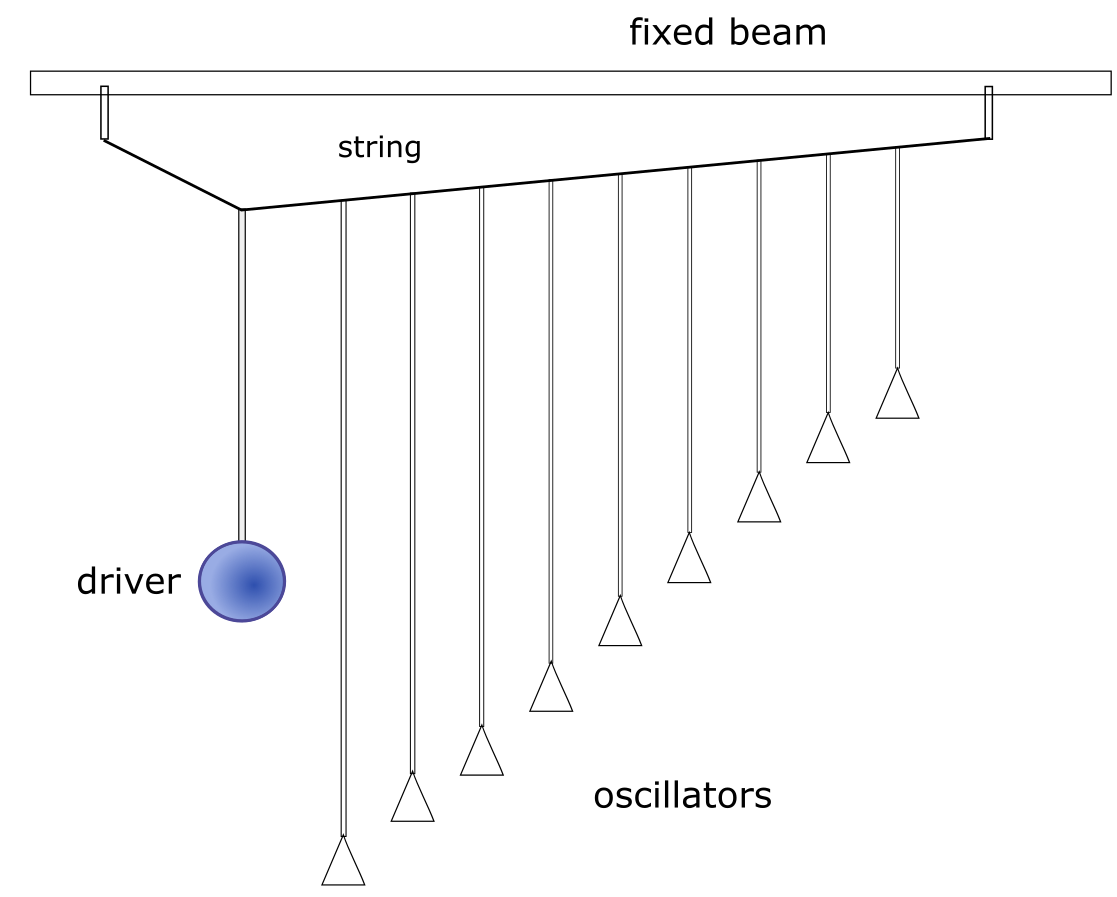
\includegraphics[width = 0.6\textwidth]{figures/chapter04/bartons_pendulums.png}
    \vspace{-15pt}
    \caption{A diagram of the Barton's pendulums experiment (courtesy Wikipedia).}
    \vspace{-10pt}
    \label{fig:bartons_pendulums}
\end{figure}

Resonant absorption is essential in the field of coronal seismology. Coronal seismology is a technique which enables solar physicists to infer coronal quantities (e.g. plasma density or magnetic field strength) by studying observed MHD waves. The technique usually involves recording data that can be measured relatively easily, e.g. wave period, wavelength, amplitude, damping time and then using MHD wave theory to infer harder to measure quantities like the magnetic field strength or density gradient. Resonant absorption can play a key role in damping observed coronal loop oscillations \citep{Nakariakov1999, Terradas2006}. \citet{Ruderman2002} shows that a kink wave in a cylindrical wave can mode convert to a torsional Alfv\'en wave. This results in the amplitude of the kink wave following a decay profile closely resembling that of observed decay profiles. Also, resonant absorption leads to the development of short length scales through phase mixing, leading to heating. \citet{Poedts1989,Ofman1995} suggest that resonant absorption could explain coronal heating. However, \citet{Prokopyszyn2019b} argue that the heating rate is too slow for observed wave amplitudes and frequencies.

This chapter focuses on studying resonant absorption when the background magnetic field is oblique to the boundary. In \citet{Halberstadt1993,Halberstadt1995} they modelled resonant absorption in the corona and showed that tilting the background magnetic field and imposing line-tied boundary conditions causes the formation of evanescent fast wave boundary layers. These boundary layers have also been studied numerically in \citet{Arregui2003}. Since the evanescent fast waves form at the boundary, we believe it is worth checking the validity of the boundary conditions. To test the validity, we check if a model where the chromosphere is included instead of imposing line-tied boundary conditions can still produce the same evanescent fast waves. We believe we are the first authors to study the boundary layers in a model where the chromosphere and corona are included. The corona and chromosphere are modelled using a piecewise constant background density profile with a discontinuous jump from the corona to the chromosphere.

Previous chapters injected waves using a footpoint driver, whereas, this chapter drives from the side for mathematical convenience. Instead of studying how waves enter the corona, we study their dynamics after entering the corona. How waves are generated in the corona remains an open question. The exponential density and the steep jump in density at the transition region make it difficult for Alfv\'en waves generated at the photosphere to enter the corona \citep{Cranmer2005}. \citet{Hollweg1984b} suggests resonances in coronal loops and spicules provide enough energy flux to the corona. \citet{Cally2011,Hansen2012} suggest that mode conversion from fast waves to Alfv\'en waves at the transition region enables sufficient energy flux to enter the corona. It is also possible that the corona itself generates Alfv\'en waves via magnetic reconnection \citep{Cranmer2018}.

In this chapter, we start by giving a general overview of the model and the equations we will use in Sections \ref{sec:chap_4_model_and_eqns} and \ref{sec:chap_4_energy_equations}. However, we make small changes to the model throughout the chapter. Section \ref{sec:normal_field_resonant_absorption_with_line_tied_bcs} introduces some of the key and most relevant properties of resonant absorption in a simple domain where the background magnetic field is perpendicular to the $z=z_{min}$ and $z=z_{max}$ boundaries. In Section \ref{sec:oblique_field_uniform_density_profile_with_line_tied_bcs} we model the background magnetic field as oblique to the boundaries and we calculate normal mode solutions in a domain where the Alfv\'en speed is uniform. We impose an incident Alfv\'en wave and calculate the unique solution which ensures the velocity is zero at $z=0$. Since the Alfv\'en speed is uniform, resonant absorption cannot occur. However, we choose very short length scales in $x$ to simulate the conditions near a singularity in a resonant absorption experiment. Section \ref{sec:oblique_field_piecewise_constant_density_profile} builds on Section \ref{sec:oblique_field_uniform_density_profile_with_line_tied_bcs} by using a piecewise constant in $z$ background Alf\'en speed. The regions $z>0$ and $z<0$ corresponds to the corona and chromosphere respectively. We impose an incident Alfv\'en wave and calculate the unique solution which ensures continuity of the velocity and its derivative at $z=0$. By comparing results from Sections \ref{sec:oblique_field_uniform_density_profile_with_line_tied_bcs} and \ref{sec:oblique_field_piecewise_constant_density_profile} we can test if the boundary layers produced by line-tied boundary conditions are physical. In Section \ref{sec:oblique_field_resonant_absorption} we use a background Alfv\'en speed which is a function of $x$ and piecewise constant in $z$. Our goal here is to test if steep boundary layers form in a resonant absorption experiment. Finally, in Section \ref{sec:chap_4_conclusions} a summary of our results and conclusions are given.

% we consider the case where the magnetic field to be oblique to the boundary. Section \ref{sec:oblique_field_piecewise_constant_density_profile} builds on Section  we consider the case where the Alfv\'en speed is uniform in $x$ as our goal is to understand why the boundary layers form at the transition region in as simple a domain as possible. Section \ref{sec:oblique_field_resonant_absorption} builds on Section \ref{sec:oblique_field_piecewise_constant_density_profile} by modelling the case where the Alfv\'en speed is a function of $x$ as this is necessary for resonant absorption to occur. Finally in Section \ref{sec:oblique_field_uniform_density_profile_with_line_tied_bcs} we consider the case where line-tied boundary conditions are used to test if the magnitude of the boundary layers which are formed when line-tied boundary conditions are used is physical and approximately agrees with the solution when the chromosphere is included in the model.

\section{Model and equations}
\label{sec:chap_4_model_and_eqns}

In this section we describe the most general model we use. However, throughout this chapter aspects of the model will change. For example, in Section \ref{sec:oblique_field_uniform_density_profile_with_line_tied_bcs} and \ref{sec:oblique_field_piecewise_constant_density_profile} the background Alfv\'en speed is independent of $x$.

We model perturbations on a static background equilibrium and make the same assumptions as those described by Equation \eqref{eq:linear_assumotion_v}-\eqref{eq:linear_assumotion_rho}. The system is assumed to be ideal, i.e. we neglect viscosity and resistivity. We model the plasma as cold, i.e. $\beta=0$, which means the magnetic pressure force is negligible. We assume the Lorentz force dominates and neglect the gravitational force. The background magnetic field is at an angle $\alpha$ to the $z$-axis in the $y$-$z$ plane, i.e.
\begin{equation}
    \label{eq:chap_4_background_field}
    \begin{aligned}
    \vec{B}_0 &= B_0(\sin\alpha\,\vec{\hat{y}}+\cos\alpha\,\vec{\hat{z}}) \\
    &= B_0\vec{\hat{B}}_0,
    \end{aligned}
\end{equation}
The unit vectors, $\vec{\hat{B}}_0$ and $\vec{\hat{\perp}}$, are defined as
\begin{gather}
    \vec{\hat{B}}_0 = \sin\alpha\,\vec{\hat{y}}+\cos\alpha\,\vec{\hat{z}}, \\
    \vec{\hat{\perp}} = \cos\alpha\,\vec{\hat{y}}-\sin\alpha\,\vec{\hat{z}},
\end{gather}
where both unit vectors are in the $y$-$z$ plane, $\vec{\hat{B}}_0$ is parallel to the background magnetic field and $\vec{\hat{\perp}}$ is perpendicular to the background magnetic field. 
The background Alfv\'en speed is given by $v_A(x,z) = \hat{v}_A(x)v_{A}(0,z)$, where
\begin{equation}
    \label{eq:chap_4_vA(0,z)}
    v_A(0,z)= \begin{cases}
    v_{A-}, & z < 0, \\
    v_{A+}, & z \ge 0,
    \end{cases}
\end{equation}
and $\hat{v}_A(x)$ is an arbitrary function of $x$ satisfying $\hat{v}_A(0)=1$. The region $z<0$ models the chromosphere and the region $z>0$ models the corona, therefore, $v_{A+}>v_{A-}$ due to the higher density in the chromosphere.

The variables we solve for are the velocity, $\vec{u}$, given by
\begin{equation}
    \vec{u}(x,y,z) = u_x\vec{\hat{x}} + u_\perp \vec{\hat{\perp}}
\end{equation}
and the magnetic field perturbations, $\vec{b}$, given by
\begin{equation}
    \vec{b}(x,y,z) = b_x\vec{\hat{x}} + b_\perp \vec{\hat{\perp}} + b_{||}\vec{\hat{B}}_0,
\end{equation}
where
\begin{equation}
\begin{aligned}
    \vec{\hat{b}}(x,y,z) &= \hat{b}_x\vec{\hat{x}} + \hat{b}_\perp \vec{\hat{\perp}} + \hat{b}_{||}\vec{\hat{B}}_0 \\
    &= \frac{\vec{b}}{B_0}.
\end{aligned}
\end{equation}

The linearised momentum equation simplifies to
\begin{equation}
    \label{eq:chap_4_linearised_momentum_eqn}
    \begin{aligned}
        \pdv{\vec{u}}{t}=\frac{1}{\mu\rho(x,z)}\qty[(\vec{B}_0\cdot\grad)\vec{b} - \grad\qty(\vec{b}\cdot\vec{B}_0)],
    \end{aligned}
\end{equation}
and the induction equation simplifies to
\begin{equation}
    \label{eq:chap_4_linearised_induction_eqn}
    \begin{aligned}
    \pdv{\vec{b}}{t}=(\vec{B}_0\cdot\grad)\vec{u} - \vec{B}_0\div{\vec{u}}.
    \end{aligned}
\end{equation}
Written out component-wise the above equations become
\begin{gather}
    \label{eq:chap_4_ux_eqn1}
    \pdv{u_x}{t}=v_A^2(x,z)\left[\nabla_{||}\hat{b}_x - \pdv{\hat{b}_{||}}{x}\right],\\
    \label{eq:chap_4_u_perp_eqn1}
    \pdv{u_\perp}{t}=v_A^2(x,z)\left[\nabla_{||}\hat{b}_\perp-\nabla_\perp \hat{b}_{||}\right],\\
    \label{eq:chap_4_bx_eqn1}
    \pdv{\hat{b}_x}{t}=\nabla_{||}u_x,\\
    \label{eq:chap_4_b_perp_eqn1}
    \pdv{\hat{b}_\perp}{t}=\nabla_{||}u_{\perp},\\
    \label{eq:chap_4_b_par_eqn1}
    \pdv{\hat{b}_{||}}{t}=-\left[\pdv{u_x}{x}+\nabla_\perp u_{\perp}\right],
\end{gather}
where
\begin{gather}
    \label{eq:nabla_perp}
    \begin{aligned}
    \nabla_\perp &= \vec{\hat{\perp}}\vdot\grad \\
    &= \cos\alpha\pdv{}{y}-\sin\alpha\pdv{}{z},
    \end{aligned} \\
    \label{eq:nabla_par}
    \begin{aligned}
    \nabla_{||} &= \vec{\hat{B}}_0\vdot\grad \\
    &= \sin\alpha\pdv{}{y}+\cos\alpha\pdv{}{z},
    \end{aligned}
\end{gather}
are the derivatives perpendicular and parallel to the
equilibrium magnetic field respectively.

\section{Energy equations}
\label{sec:chap_4_energy_equations}

Resonant absorption occurs due to fast waves mode converting into Alfv\'en waves at a resonant field line. This can be better understood by considering how the oscillations in the $x$ and $\vec{\hat{B}}_0$ direction couple to the fluctuations in the $\perp$-direction. Note that the $x$ and $||$ perturbation energy density is given by
\[\frac{1}{2}\rho u_x^2 + \frac{b_x^2}{2\mu} + \frac{b_{||}^2}{2\mu},\]
and the $\perp$-energy density is given by
\[\frac{1}{2}\rho u_\perp^2 + \frac{b_\perp^2}{2\mu} .\]

Taking the dot product of Equation \eqref{eq:chap_4_linearised_momentum_eqn} with $\vec{u}_x=u_x\vec{\hat{x}}$ gives
\[\pdv{}{t}\left(\frac{1}{2}\rho u_x^2\right)=\frac{1}{\mu}[(\vec{B}_0\cdot\vec{\nabla})b_x]u_x-\frac{B_0}{\mu}\pdv{b_{||}}{x}u_x.\]
Taking the dot product of Equation \eqref{eq:chap_4_linearised_momentum_eqn} with $\vec{b}_x=b_x\vec{\hat{x}}$ gives
\[\pdv{}{t}\left(\frac{b_x^2}{2\mu}\right)=\frac{1}{\mu}[(\vec{B}_0\cdot\vec{\nabla})u_x]b_x.\]
Note that,
\[\vec{\nabla}\cdot\left(\frac{\vec{E}\times\vec{b}_x}{\mu}\right)=-\frac{1}{\mu}\vec{B}_0\cdot\vec{\nabla}(u_xb_x),\]
hence,
\begin{equation}
    \label{eq:chap_4_x_energy}
    \pdv{}{t}\left(\frac{1}{2}\rho u_x^2+\frac{b_x^2}{2\mu}\right)+\vec{\nabla}\cdot\left(\frac{\vec{E}\times\vec{b}_x}{\mu}\right)=-\frac{B_0}{\mu}u_x\pdv{b_{||}}{x}.
\end{equation}
Similarly, we can show that
\begin{gather}
    \label{eq:chap_4_perp_energy}
    \pdv{}{t}\left(\frac{1}{2}\rho u_\perp^2+\frac{b_\perp^2}{2\mu}\right)+\vec{\nabla}\cdot\left(\frac{\vec{E}\times\vec{b}_\perp}{\mu}\right)=-\frac{B_0}{\mu}u_\perp\nabla_\perp b_{||}, \\
    \label{eq:chap_4_par_energy}
    \pdv{}{t}\left(\frac{b_{||}^2}{2\mu}\right)+\vec{\nabla}\cdot\left(\frac{\vec{E}\times\vec{b}_{||}}{\mu}\right)=\frac{B_0}{\mu}(\vec{u}\cdot\vec{\nabla})b_{||}.
\end{gather}
Adding Equation \eqref{eq:chap_4_x_energy} to \eqref{eq:chap_4_par_energy} gives
\begin{equation}
    \label{eq:chap_4_fast_energy}
    \pdv{}{t}\left(\frac{1}{2}\rho u_x^2+\frac{b_x^2+b_{||}^2}{2\mu}\right)+\vec{\nabla}\cdot\left[\frac{\vec{E}\times(\vec{b}_x+\vec{b}_{||})}{\mu}\right]=\frac{B_0}{\mu}u_\perp\nabla_\perp b_{||}.
\end{equation}
% In this chapter, we can think of Equations \eqref{eq:chap_4_fast_energy} and as describing the evolution of the fast wave energy and Alfv\'en wave energies respectively because we will show in for example.
Equations \eqref{eq:chap_4_perp_energy} and \eqref{eq:chap_4_fast_energy} show that gradients in the magnetic pressure, $B_0b_{||}/\mu$, are responsible for the mode conversion from oscillations in the $x$, $||$ directions to oscillations in the $\perp$ direction. If $\nabla_\perp = 0$ then no mode conversion can occur between the fast and Alfv\'en waves and they are independent of one another.

\section{Normal field: Resonant absorption with line-tied BCs}
\label{sec:normal_field_resonant_absorption_with_line_tied_bcs}

This section aims to introduce resonant absorption by calculating the solution for the simple case where $\alpha=0$. Therefore, the background magnetic field points in the $z$-direction. We aim to show how the waves can form very short length-scales if the system has a relatively small gradient in Alfv\'en travel time across the background magnetic field lines.

\subsection{Equations}

For simplicity, we will model the chromosphere as infinitely denser than the corona, i.e. $v_{A-}\rightarrow 0$. We will model the $z$-range as $0\le z\le L_z$ and impose line-tied boundary conditions at $z=0$ and $z=L_z$, i.e. 
\begin{equation}
    u_x|_{z=0}=u_x|_{z=L_z}=u_y|_{z=0}=u_y|_{z=L_z}=0.
\end{equation}
Therefore, $v_A=v_A(x)$. The $x$ domain is given by $x\ge x_{min}$ and we impose a driver at $x=x_{min}$, of the form
\begin{gather}
    \label{eq:chap_4_x_min_bcs_alpha=0}
    u_x(x_{min},y,z,t) = f_{driv}(y,z,t), \\
    \left.\pdv{u_x}{x}\right|_{x=x_{min}} = g_{driv}(y,z,t).
\end{gather}

Since $\alpha=0$, this means that $u_y = u_\perp$, $b_y = b_{\perp}$ and $b_z = b_{||}$. Also, $\nabla_\perp=\pdv*{}{y}$ and $\nabla_{||}=\pdv*{}{z}$. Therefore, Equations \eqref{eq:chap_4_ux_eqn1}-\eqref{eq:chap_4_b_par_eqn1} can be written as
\begin{gather}
    \label{eq:chap_4_ux_eqn_alpha=0}
    \pdv{u_x}{t} = v_A^2(x)\qty[\pdv{\hat{b}_x}{z} - \pdv{\hat{b}_z}{x}],\\
    \pdv{u_y}{t} = v_A^2(x)\qty[\pdv{\hat{b}_y}{z} - \pdv{\hat{b}_z}{y}],\\
    \pdv{\hat{b}_x}{t} = \pdv{u_x}{z},\\
    \pdv{\hat{b}_y}{t} = \pdv{u_y}{z},\\
    \label{eq:chap_4_bz_eqn_alpha=0}
    \pdv{\hat{b}_z}{t} = -\qty[\pdv{u_x}{x} + \pdv{u_y}{y}].
\end{gather}

\subsection{Analytic solution}
\label{sec:chap_4_normal_mode_analytic_solution}

The problem is linear and the functions we need to solve for depend on just $x$. Therefore, by assuming a Fourier solution in $y$, $z$ and $t$ we can convert the PDEs, \eqref{eq:chap_4_ux_eqn_alpha=0}-\eqref{eq:chap_4_bz_eqn_alpha=0} into a set of ODEs.
We assume the solutions are of the form
\begin{gather}
    \label{eq:chap_4_ux_expansion}
    u_x(x,y,z,t) = \sum_{n=1}^\infty u_{xn}(x)\sin(k_{zn}z)\exp[i(k_y y + \omega t)], \\
    u_y(x,y,z,t) = \sum_{n=1}^\infty u_{yn}(x)\sin(k_{zn}z)\exp[i(k_y y + \omega t)], \\
    \hat{b}_x(x,y,z,t) = \sum_{n=1}^\infty \hat{b}_{xn}(x)\sin(k_{zn}z)\exp[i(k_y y + \omega t)], \\
    \hat{b}_y(x,y,z,t) = \sum_{n=1}^\infty \hat{b}_{yn}(x)\sin(k_{zn}z)\exp[i(k_y y + \omega t)], \\
    \label{eq:chap_4_bz_expansion}
    \hat{b}_z(x,y,z,t) = \sum_{n=1}^\infty \hat{b}_{zn}(x)\sin(k_{zn}z)\exp[i(k_y y + \omega t)],
\end{gather}
where $k_y$, $\omega$ are constants,
\begin{equation}
    k_{zn} = \frac{n\pi}{L_z},
\end{equation}
this ensures the line-tied boundary conditions in $z$ are automatically satisfied. Substituting the above series into Equations \eqref{eq:chap_4_ux_eqn_alpha=0}-\eqref{eq:chap_4_bz_eqn_alpha=0}, and multiplying by $\sin(k_{zm}z)$ and integrating from $0$ to $L_z$ gives.
\begin{gather}
    i\omega u_{xm} = v_A^2(x)\qty[ik_{zm} \hat{b}_{xm} - \dv{\hat{b}_{zm}}{x}],\\
    i\omega u_{ym} = v_A^2(x)\qty[ik_{zm} \hat{b}_{xm} - ik_y \hat{b}_{zm}],\\
    i\omega \hat{b}_{xm} = ik_{zm}u_{xm},\\
    i\omega \hat{b}_{ym} = ik_{zm}u_{ym},\\
    \label{eq:chap_4_bz_eqn2_alpha=0}
    i\omega \hat{b}_{zm} = -\qty[\dv{u_{xm}}{x}+ ik_yu_{ym}].
\end{gather}
Let
\begin{equation}
    \mathcal{L}_n(x) = \frac{\omega^2}{v_A^2(x)} - k_{zn}^2.
\end{equation}
Eliminating $\hat{b}_{xn}$ and $\hat{b}_{yn}$ gives
\begin{gather}
   \mathcal{L}_n(x)u_{xn}(x)=i\omega \dv{\hat{b}_{zn}}{x}, \\
   \label{eq:chap_4_uy_eqn_bz}
   \mathcal{L}_n(x)u_{yn}(x)=ik_y i\omega \hat{b}_{zn}.
\end{gather}
Eliminating $\hat{b}_{zn}$ gives
\begin{gather}
    \label{eq:chap_4_ux_eqn2_alpha=0}
    \dv[2]{u_{xn}}{x}+\mathcal{L}_n(x)u_{xn}(x)=-ik_y\dv{u_{yn}}{x},\\
    \label{eq:chap_4_uy_eqn2_alpha=0}
    \qty[\mathcal{L}_n(x)-k_y^2]u_{yn}(x)=-ik_y\dv{u_{xn}}{x}.
\end{gather}
Eliminating $u_{yn}$ from Equation \eqref{eq:chap_4_ux_eqn2_alpha=0}, using Equation \eqref{eq:chap_4_uy_eqn2_alpha=0}, gives
\[
    \begin{aligned}
    \dv[2]{u_{xn}}{x}+\mathcal{L}_n(x)u_{xn}(x)&=-ik_y\dv{}{x}\qty[\frac{-ik_y}{\mathcal{L}_n(x)-k_y^2}\dv{u_{xn}}{x}] \\
    &=\frac{-k_y^2}{\mathcal{L}_n(x)-k_y^2}\qty[\dv[2]{u_{xn}}{x}-\frac{\mathcal{L}_x(x)}{\mathcal{L}_n(x)-k_y^2}\dv{u_{xn}}{x}],
    \end{aligned}
\]
where
\begin{gather}
\begin{aligned}
    \mathcal{L}_x(x) &= \dv{\mathcal{L}_n}{x} \\
    &= -2\frac{\omega^2}{v_A^3(x)}\dv{v_A}{x} \\
    &= -\frac{2\omega^2}{v_A^2(x)a(x)},
\end{aligned} \\
    \tag{\ref{eq:length_scale_alfven_travel_time}}
    a(x) = \frac{v_A(x)}{\dv*{v_A}{x}}.
\end{gather}
Rearranging gives
\begin{equation}
    \label{eq:uxn_ode1}
    \mathcal{L}_n(x)\dv[2]{u_{xn}}{x}-\frac{k_y^2\mathcal{L}_x(x)}{\mathcal{L}_n(x)-k_y^2}\dv{u_{xn}}{x}+\mathcal{L}_n(x)[\mathcal{L}_n(x)-k_y^2]u_{xn}(x)=0.
\end{equation}

We can eliminate $u_x$ to get an equation for $u_\perp$ via the following procedure. Take the $x$-derivative of Equation \eqref{eq:chap_4_ux_eqn2_alpha=0} to give
\[
    u_{xn}(x) = -\frac{1}{\mathcal{L}_n'(x)}\qty{\qty[\dv[2]{}{x}+\mathcal{L}_n]\dv{u_{xn}}{x}+ik_y\dv[2]{u_{yn}}{x}}.
\]
Substitute this into Equation \eqref{eq:chap_4_ux_eqn2_alpha=0} to give
\[
    \dv[2]{u_{xn}}{x}-\frac{\mathcal{L}_n}{\mathcal{L}_x}\qty{\qty[\dv[2]{}{x}+\mathcal{L}_n]\dv{u_{xn}}{x}+ik_y\dv[2]{u_{yn}}{x}}=-ik_y\dv{u_{yn}}{x},
\]
where we have assumed $\mathcal{L}_x(x)\ne0$. See for example \citet{Thompson1993} for a calculation of the solution in the case where $\mathcal{L}_n(x)=\mathcal{L}_x(x)=0$.
Multiply through by $-ik_y$ and eliminate $u_{xn}$ using Equation \eqref{eq:chap_4_uy_eqn2_alpha=0} to give
\[
\begin{aligned}
    &\dv{}{x}[(\mathcal{L}_n-k_y^2)u_{yn}]-\\
    &\frac{\mathcal{L}_n}{\mathcal{L}_x(x)}\qty{\qty[\dv[2]{}{x}+\mathcal{L}_n]\qty[\mathcal{L}_n-k_y^2]u_{yn}+k_y^2\dv[2]{u_{yn}}{x}}=-k_y^2\dv{u_{yn}}{x}.
\end{aligned}
\]
This can be simplified to give
\begin{equation}
\label{eq:chap_4_uy_ode}
    \mathcal{L}_n^2\dv[2]{u_{yn}}{x}+\mathcal{L}_x\mathcal{L}_n\dv{u_{yn}}{x}+(\mathcal{L}_n^3+\mathcal{L}_{xx}\mathcal{L}_n-k_y^2\mathcal{L}_n-\mathcal{L}_x^2) u_{yn}=0,
\end{equation}
where
\begin{equation}
    % \mathcal{M}_n = \mathcal{L}_n^3+\mathcal{L}_{xx}\mathcal{L}_n-k_y^2\mathcal{L}_n-\mathcal{L}_x^2, \\
    \mathcal{L}_{xx} = \dv{\mathcal{L}_x}{x}.
\end{equation}

Our goal now is to solve Equations \eqref{eq:uxn_ode1} and \eqref{eq:chap_4_uy_ode} using the method of Frobenius. Assume that $\mathcal{L}_n$ is an analytic function. Therefore, points where $\mathcal{L}_n(x)\ne0$ are ordinary/regular points of Equation \eqref{eq:chap_4_uy_ode} and points where $\mathcal{L}_n(x)=0$ are regular-singular points of the ODE. Let $x_{res,n}$ be defined as a point satisfying $\mathcal{L}_n(x_{res,n})=0$. If multiple points satisfy $\mathcal{L}_n(x)=0$, then pick $x_{res,n}$ equal to one of these points arbitrarily. Since we expect solutions $u_{yn}$ to be singular at $x=x_{res,n}$, we will focus on studying solutions near this point.

\subsubsection{Radius of convergence}

Multiplying Equation \eqref{eq:uxn_ode1} through by $(x-x_{res,n})^2/\mathcal{L}_n(x)$ gives
\begin{equation}
    \label{eq:uxn_ode2}
    (x-x_{res,n})^2\dv[2]{u_{xn}}{x} + (x-x_{res,n})p_n(x)\dv{u_{xn}}{x} + q_n(x)u_{xn}(x)=0,
\end{equation}
where
\begin{gather}
    p_n(x) = -\frac{k_y^2\mathcal{L}_x(x)(x-x_{res,n})}{\mathcal{L}_n(x)(\mathcal{L}_n(x)-k_y^2)}, \\
    q_n(x) = (\mathcal{L}_n(x)-k_y^2)(x-x_{res,n})^2.
\end{gather}
The power series solution for $u_{xn}$ about $x=x_{res,n}$ will have a radius of convergence at least as large as the radius of convergence for the power series of $p_n(x)$ and $q_n(x)$ about $x=x_{res,n}$. Since $\mathcal{L}_n(x)$ is analytic we expect the radius of convergence for $q_n$ to be infinite. The radius of convergence of $p_n(x)$ (denoted with $R_n$) is equal to the distance in the complex plane between $x_{res,n}$ and the nearest zero of $\mathcal{L}_n(x)(\mathcal{L}_n(x)-k_y^2)$ (excluding the point $x=x_{res,n}$). Hence, the radius of convergence for $u_{xn}$ about $x=x_{res,n}$ is at least as large as $R_n$.

\subsubsection{Indicial polynomial}

To calculate the solution via the method of Frobenius we first need to calculate the indicial polynomial. Substituting
\[u_{xn}(x)=(x-x_{res,n})^\sigma\sum_{k=0}^\infty a_k(x-x_{res,n})^k,\]
into Equation \eqref{eq:uxn_ode2} gives
\[\sum_{k=0}^\infty [(k + \sigma - 1)(k+\sigma) + (k+\sigma)p_n(x) + q_n(x)]a_k(x-x_{res,n})^k=0.\]
We need to find values of $\sigma$ where non-trivial solutions can exist.
Taylor expanding $p(x)$ and $q(x)$ about $x=x_{res,n}$, we calculate the coefficient of the leading order power in $(x-x_{res,n})$ to be given by
\begin{equation}
    I(\sigma) = (\sigma-1)\sigma + p_n(x_{res,n})\sigma + q_n(x_{res,n}),
\end{equation}
where $I(\sigma)$ is the indicial polynomial. Since $I(\sigma)=0$, $p_n(x_{res,n})=1$ and $q_n(x_{res,n})=0$ we know that $\sigma^2=0$. Since we have repeated roots the general solution  is given by a linear combination of
\begin{equation}
    u_{xn1}(x) = \sum_{k=0}^\infty a_k(x-x_{res,n})^k,
\end{equation}
and
\begin{equation}
    u_{xn2}(x) = u_{xn1}(x)\ln(x-x_{res,n}) + \sum_{k=1}^\infty b_k(x-x_{res,n})^k.
\end{equation}

\subsubsection{Recurrence relations}

We will now calculate the recurrence relation for the $a_k$ terms. Substituting $u_{xn1}(x)$ into Equation \eqref{eq:uxn_ode2} and Taylor expanding $p_n(x)$ and $q_n(x)$ about $x=x_{res,n}$ gives
\[\sum_{k=0}^\infty\qty[I(k)a_k+\sum_{j=0}^{k-1}\frac{jp_n^{(k-j)}(x_{res,n})+q_n^{(k-j)}(x_{res,n})}{(k-j)!}a_j] \qty(x-x_{res,n})^k=0.\]
Equating the coefficient of $(x-x_{res,n})^k$ equal to zero gives the following recurrence relation,
\begin{equation}
    a_k = -\frac{1}{I(k)}\sum_{j=0}^{k-1}\frac{jp_n^{(k-j)}(x_{res,n})+q_n^{(k-j)}(x_{res,n})}{(k-j)!}a_j,
\end{equation}
for $k\ge1$, where we arbitrarily set $a_0=1$. Setting $a_0=1$ does not lose generality as $u_{xn}$ is equal to a linear combination of $u_{xn1}$ and $u_{xn2}$. Since $q_n'(x_{res,n})=0$ we know that $a_1=0$.

We will now calculate an expression for the $b_k$ terms. Note that
\[\dv{u_{xn2}}{x} = \dv{u_{xn1}}{x}\ln(x-x_{res,n}) + \frac{u_{xn1}}{x-x_{res,n}} + \sum_{k=1}^\infty kb_k(x-x_{res,n})^{k-1},\]
\[\begin{aligned}
\dv[2]{u_{xn2}}{x} &= \dv[2]{u_{xn1}}{x}\ln(x-x_{res,n}) + \frac{2}{x-x_{res,n}}\dv{u_{xn1}}{x} - \frac{u_{xn1}}{(x-x_{res,n})^2} \\
&+ \sum_{k=1}^\infty k(k-1)b_k(x-x_{res,n})^{k-2}.
\end{aligned}\]
Hence, substituting $u_{xn2}(x)$ into Equation \eqref{eq:uxn_ode2} gives
\[\begin{aligned}
&2(x-x_{res,n})\dv{u_{xn1}}{x}+[p_n(x) - 1]u_{xn1}(x) + \\
&\qquad\sum_{k=1}^\infty[k(k - 1) + kp_n(x) + q_n(x)]b_k(x-x_{res,n})^k = 0.
\end{aligned}\]
Substituting for $u_{xn1}(x)$ gives
\[\begin{aligned}
&\sum_{k=0}^\infty[2k + p_n(x) - 1]a_k(x-x_{res,n})^k + \\
&\qquad\sum_{k=1}^\infty [k(k - 1) + kp_n(x) + q_n(x)]b_k(x-x_{res,n})^k = 0.
\end{aligned}\]
Taylor expanding $p_n(x)$, $q_n(x)$ about $x=x_{res,n}$ gives
\[\begin{aligned}
&\sum_{k=0}^\infty\qty[(2k + p_n(0) - 1)a_k + \sum_{j=0}^{k-1}\frac{p_n^{(k-j)}(x_{res,n})}{(k-j)!}a_j] \qty(x-x_{res,n})^k + \\
&\qquad\sum_{k=1}^\infty \qty[I(k)b_k + \sum_{j=1}^{k-1}\frac{jp_n^{(k-j)}(x_{res,n})+q_n^{(k-j)}(x_{res,n})}{(k-j)!}b_j] \qty(x-x_{res,n})^k = 0.
\end{aligned}\]
Equating the coefficient of $(x-x_{res,n})^k$ equal to zero gives
% \begin{equation}
%     \begin{aligned}
%     a_0 &= \frac{p_n'(x_{res,n})-q_n'(x_{res,n})}{I(0)}a_{-1} \\
%         &= \frac{4\mathcal{L}_{xx}(x_{res,n}) - k_y^2}{\mathcal{L}_x(x_{res,n})}a_{-1}
%     \end{aligned}
% \end{equation}
% where,
% Equating the coefficient of $(x-x_{res,n})^1$ equal to zero gives
% \[2Ca_1+\sum_{j=-1}^0\frac{jp_n^{(1-j)}(x_{res,n})+q_n^{(1-j)}(x_{res,n})}{(1-j)!}b_j=0,\]
% hence, $C$ is given by
% \begin{equation}
%     C=-\frac{1}{2a_1}\sum_{j=-1}^0\frac{jp_n^{(1-j)}(x_{res,n})+q_n^{(1-j)}(x_{res,n})}{(1-j)!}b_j=0,
% \end{equation}
% for $a_1\ne0$. If $a_1=0$ then $C$ can be arbitrary. Equating the coefficient of $(x-x_{res,n})^k$ for $k\ge1$ gives the following recurrence relation
\begin{equation}
\begin{aligned}
    -I(k)b_k &= (2k + p_n(0) - 1)a_k + \sum_{j=0}^{k-1}\frac{p_n^{(k-j)}(x_{res,n})}{(k-j)!}a_j \\
    &+ \sum_{j=1}^{k-1}\frac{jp_n^{(k-j)}(x_{res,n})+q_n^{(k-j)}(x_{res,n})}{(k-j)!}b_j,
\end{aligned}
\end{equation}
for $k\ge1$. Since $a_1=0$ and $a_0=1$ we know that $b_1$ is given by
\begin{equation}
    b_1 = -p_n'(x_{res,n}).
\end{equation}

\subsubsection{Singular solutions}

Our goal now is to calculate the leading order singular solutions for $u_{xn}$, $u_{y n}$ and $b_{zn}$. Note that if $\omega\in\mathds{C}$ then $x_{res,n}\in\mathds{C}$. Let $x_{res,n}=x_{r,n} + i x_{i,n}$, where $x_{r,n},x_{i,n}\in \mathds{R}$. We will assume that $\abs{x_{i,n}}\ll R_n$. Let $u_{xn}$ be given by
\begin{equation}
\label{eq:uxn_leading_order_solution}
\begin{aligned}
    u_{xn}(x) &= -iu_0 x_{i,n} k_y\qty[u_{xn2}(x) - u_{xn1}(x)\ln(x_{i,n})] \\
    &= -iu_0 x_{i,n} k_y \qty[\ln(X_n)+ x_{i,n}b_1X_n + O(X_n^2\ln X_n,X_n^2)],
\end{aligned}
\end{equation}
where
\begin{equation}
    X_n = \frac{x-x_{res,n}}{x_{i,n}}.
\end{equation}

From Equation \eqref{eq:chap_4_uy_eqn2_alpha=0} we know that
\begin{equation}
\label{eq:uyn_leading_order_solution}
\begin{aligned}
    u_{yn}(x) &= \frac{-ik_y}{\mathcal{L}_n(x)-k_y^2}\dv{u_{xn}}{x} \\
    &=u_0\qty{\frac{1}{X_n} + x_{i,n}b_1 + \frac{\mathcal{L}_x}{k_y^2}x_{i,n} + O\qty(X_n\ln X_n, X_n)}.
\end{aligned}
\end{equation}

Substituting Equation \eqref{eq:uyn_leading_order_solution} into Equation \eqref{eq:chap_4_uy_eqn_bz} gives
\begin{equation}
\label{eq:bzn_leading_order_solution}
\begin{aligned}
    \hat{b}_{zn}(x) &= \frac{-\mathcal{L}_n(x)}{\omega k_y}u_{yn}(x) \\
    &= \frac{u_0}{v_{A}(x_{res,n})}\qty[-\frac{v_{A}(x_{res,n})\mathcal{L}_x}{\omega k_y}x_{i,n} + O\qty(X_n^2\ln X_n, X_n)] \\
    &= \frac{u_0}{v_{A}(x_{r,n})}\qty[\frac{2\omega x_{i,n}}{v_{A}(x_{r,n})a_0k_y} + O\qty(X_n^2\ln X_n, X_n)].
\end{aligned}
\end{equation}

\subsubsection{Poynting flux}

One of the most useful quantities in coronal seismology is the wave (e.g. kink wave) damping time \citep{Ruderman2002, Giagkiozis2016}. This is related to the Poynting flux, which gives the energy flux (see Equation \ref{eq:total_energy_eqn_linear}).

Using Equation \eqref{eq:poynting_flux_linear}, the Poynting flux in the $x$-direction is given by
\begin{equation}
\begin{aligned}
    S_x &= \frac{1}{\mu}\Big\{\big[\Re(\vec{b})\vdot\vec{B}_0\big]\Re(\vec{u}) - \big[\Re(\vec{u})\vdot\Re(\vec{b})\big]\vec{B}_0\Big\}\vdot\vec{\hat{x}} \\
    &= \frac{B_0^2}{\mu}\Re(u_x)\Re(\hat{b}_z) \\
    &= \frac{B_0^2}{\mu}\qty(\frac{u_x + u_x^*}{2})\qty(\frac{\hat{b}_z+\hat{b}_z^*}{2}),
\end{aligned}
\end{equation}
where $u_x^*$ denotes the complex conjugate of $u_x$. Therefore, the component which does not time-average to zero is given by
\begin{equation}
    \label{eq:chap_4_avg_poy_flux}
    \langle S_x \rangle = \frac{B_0^2}{4\mu}\qty(u_x\hat{b}_z^* + u_x^*\hat{b}_z).
\end{equation}
Integrating in $z$ from $0$ to $L_z$ gives
\begin{equation}
    \begin{aligned}
    \int_0^{L_z}\langle S_x \rangle dz &= \frac{L_z}{2}\sum_{n=1}^\infty\frac{B_0^2}{4\mu}\qty(u_{xn}\hat{b}_{zn}^* + u_{xn}^*\hat{b}_{zn}) \\
    &= \frac{L_z}{2}\sum_{n=1}^\infty \langle S_{xn} \rangle,
    \end{aligned}
\end{equation}
where 
\begin{equation}
    \label{eq:chap_4_avg_poy_flux_nth_contribution}
    \langle S_{xn} \rangle = \frac{B_0^2}{4\mu}\qty(u_{xn}\hat{b}_{zn}^* + u_{xn}^*\hat{b}_{zn}).
\end{equation}
Using Equations \eqref{eq:uxn_leading_order_solution} and \eqref{eq:bzn_leading_order_solution}, we know,
\begin{equation}
    \begin{aligned}
    u_{xn}\hat{b}_{zn}^* &= \big[-ik_y u_0x_{i,n}\ln X_n\big]\qty[2\frac{u_0x_{i,n}\omega}{k_yv_{A}^2(x_{r,n})a(x_{r,n})}]\sin^2(k_{zn}z) + ... \\
    &= u_0\qty[-2i\frac{u_0x_{i,n}^2\omega}{v_{A}^2(x_{r,n})a(x_{r,n})}\ln(X_n) + O\qty(X_n\ln X_n, X_n)],
    \end{aligned}
\end{equation}
and
\begin{equation}
    u_{xn}^*\hat{b}_{zn} = u_0\qty[2i\frac{u_0x_{i,n}^2\omega}{v_{A}^2(x_{r,n})a(x_{r,n})}\ln(X_n^*) + O\qty(X_n\ln X_n, X_n)],
\end{equation}
where we assume that $x\in\mathds{R}$.
Therefore,
\begin{equation}
\begin{aligned}
    \label{eq:chap_4_avg_poy_flux_leading_order_alpha=0}
    \langle S_{xn} \rangle &= i\frac{B_0^2}{2\mu}\frac{u_0^2x_{i,n}^2\omega}{v_{A}^2(x_{r,n})a_{0}}\big[\ln(x-x_{res,n}^*)-\ln(x-x_{res,n})\big] + ...  \\
    &= -\frac{B_0^2}{2\mu}\frac{u_0^2x_{i,n}^2\omega}{v_{A}^2(x_{r,n})a(x_{r,n})}\big[\tan^{-1}(x_{i,n},x-x_{r,n})-\\
    &\qquad\qquad\qquad\qquad\ \ \tan^{-1}(-x_{i,n},x-x_{r,n})\big] + O(X_n\ln X_n, X_n).
\end{aligned}
\end{equation}
Note that
\[\lim_{x\rightarrow\infty}\big\{\tan^{-1}(x_{i,n},x-x_{r,n})-\tan^{-1}(-x_{i,n},x-x_{r,n})\big\}=0,\]
\[\lim_{x\rightarrow-\infty}\big\{\tan^{-1}(x_{i,n},x-x_{r,n})-\tan^{-1}(-x_{i,n},x-x_{r,n})\big\}=2\pi\,\text{sign}(x_{i,n}).\]
Hence, the jump in Poynting flux, $\Delta S_{xn}$ across $x_{res,n}$ for $\omega_i\ll\omega_r$ is given by
\begin{equation}
    \label{eq:chap_4_jump_in_poynting_flux}
    \begin{aligned}
    % \langle \Delta S_{xn}\rangle &\approx \big\langle S_{xn} \big\rangle_{x\rightarrow\infty} - \big\langle S_{xn} \big\rangle_{x\rightarrow-\infty} \\
    % &\approx \pi\frac{B_0^2}{\mu}\frac{u_{yn0}^2x_{i,n}^2\omega_r}{v_A^2(x)a(x)}\,\text{sign}(x_i).
    \langle \Delta S_{xn}\rangle = \pi\frac{B_0^2}{\mu}\frac{u_0^2x_{i,n}^2\omega_r}{v_{A}^2(x_{r,n})a(x_{r,n})}\,\text{sign}(x_{i,n}),
    \end{aligned}
\end{equation}
where $\text{sign}(x_{i,m}) = x_{i,n} / \abs{x_{i,n}}$.
% We can expect the singular solution for $u_x$ and $u_\perp$ to dominate near $x=x_{res}$ since they go to infinity as $x\rightarrow x_{res,n}$, the same is not true for $b_{||}$. Therefore, Equation \eqref{eq:chap_4_jump_in_poynting_flux} will be inaccurate for a general set of boundary condition as the regular solution for $b_{||}$ may be important depending on the boundary conditions.

% Let $x_{res,n}=x_{r,n}+ix_{i,n}$, where $x_{r,n}$, $x_{i,n}\in\mathds{R}$. Our goal now is to calculate approximate expressions for $x_{r,n}$ and $x_{i,n}$. Taylor expanding $v_A^2(x)$ at $x=x_{r,n}$, gives
% \begin{equation}
%     v_A^2(x) = v_A^2(x_{r,n}) + 2(x-x_{r,n})\frac{v_A^2(x_{r,n})}{a(x_{r,n})} + ...\,.
% \end{equation}
% Since, $\omega_i/\omega_r\ll1$ we expect $x_{res,n}$ to be close to $x_{r,n}$, such that $v_A^2(x_{res,n})$ is approximated by the first order Taylor expansion of $v_A^2(x)$ at $x=x_{r,n}$, i.e.
% \begin{equation}
%     v_A^2(x_{res,n}) \approx v_A^2(x_{r,n}) + 2ix_{i,n}\frac{v_A^2(x_{r,n})}{a(x_{r,n})}.
% \end{equation}
% Note that
% \begin{equation}
%     \frac{\omega^2}{\omega_r^2} = \frac{\omega_r^2+2i\omega_r\omega_i} {\omega_r^2} + O(\omega_i^2/\omega_r^2).
% \end{equation}
% Since, $\mathcal{L}(x_{res,n})=0$, we know that
% \[\frac{\omega^2}{\omega_r^2k_{zn}^2}=\frac{v_A^2(x_{res,n})}{\omega_r^2}, \]
% hence,
% \[\frac{\omega_r^2+2i\omega_r\omega_i}{k_{zn}^2}\approx v_A^2(x_{r,n})+2ix_{i,n}\frac{v_A^2(x_{r,n})}{a(x_{r,n})}.\]
% Taking the real part of the above equation gives
% \begin{equation}
%     v_A^2(x_{r,n}) = \frac{\omega_r^2}{k_{zn}^2},
% \end{equation}
% the imaginary part gives
% \begin{equation}
%     \label{eq:chap_4_xi_alpha=0}
%     x_{i,n} = a(x_{r,n})\frac{\omega_i}{\omega_r}.
% \end{equation}

\subsection{Numerical solution}
\label{sec:normal_mode_numerical_soln_alpha=0}

Our goal now is to verify our analytic solution numerically. We can solve Equation \eqref{eq:uxn_ode2} by integrating in $x$ using \texttt{solve\_ivp} in \citet{SciPy2020}.

We choose the Alfv\'en speed to be given by
\begin{equation}
    v_A(x)=v_{A0}\qty(1+\frac{x}{a_0}),
\end{equation}
where we assume $x>-a_0$.
The resonant locations, $x_{res,n}$ are given by
\[\mathcal{L}_n(x_{res,n})=0 \implies = v_A(x_{res,n}) = \frac{\omega}{k_{zn}},\]
therefore,
\begin{equation}
\begin{aligned}
    x_{res,n} &= a_0\qty[\frac{\omega}{v_{A0}k_{zn}} - 1].
\end{aligned}
\end{equation}
This implies that
\begin{gather}
    x_{r,n} = a_0\qty[\frac{\omega_r}{v_{A0}k_{zn}} - 1], \\
    x_{i,n} = \frac{a_0\omega_i}{v_{A0}k_{zn}}.
\end{gather}
We choose
\begin{equation}
    \begin{aligned}
    \omega_r = v_{A0}k_{z1}
    \end{aligned}
\end{equation}
and this ensures that $x_{r,1}=0$.
We set the boundary conditions in $x$ as
\begin{gather}
    u_x|_{x=x_{min}} = -ik_yu_0x_{i,1}\ln\qty(X_1)\sin(k_{z1}z)\exp[i(k_y y + \omega t)], \\
    \left.\pdv{u_x}{x}\right|_{x=x_{min}}=-\frac{ik_yu_0}{X_1}\sin(k_{z1}z)\exp[i(k_y y + \omega t)].
\end{gather}
These boundary conditions ensure that $u_{xn}=u_{yn}=\hat{b}_{zn}=0$, $\forall n\ne 1$.

\begin{figure}
    \centering
    \vspace{-30pt}
    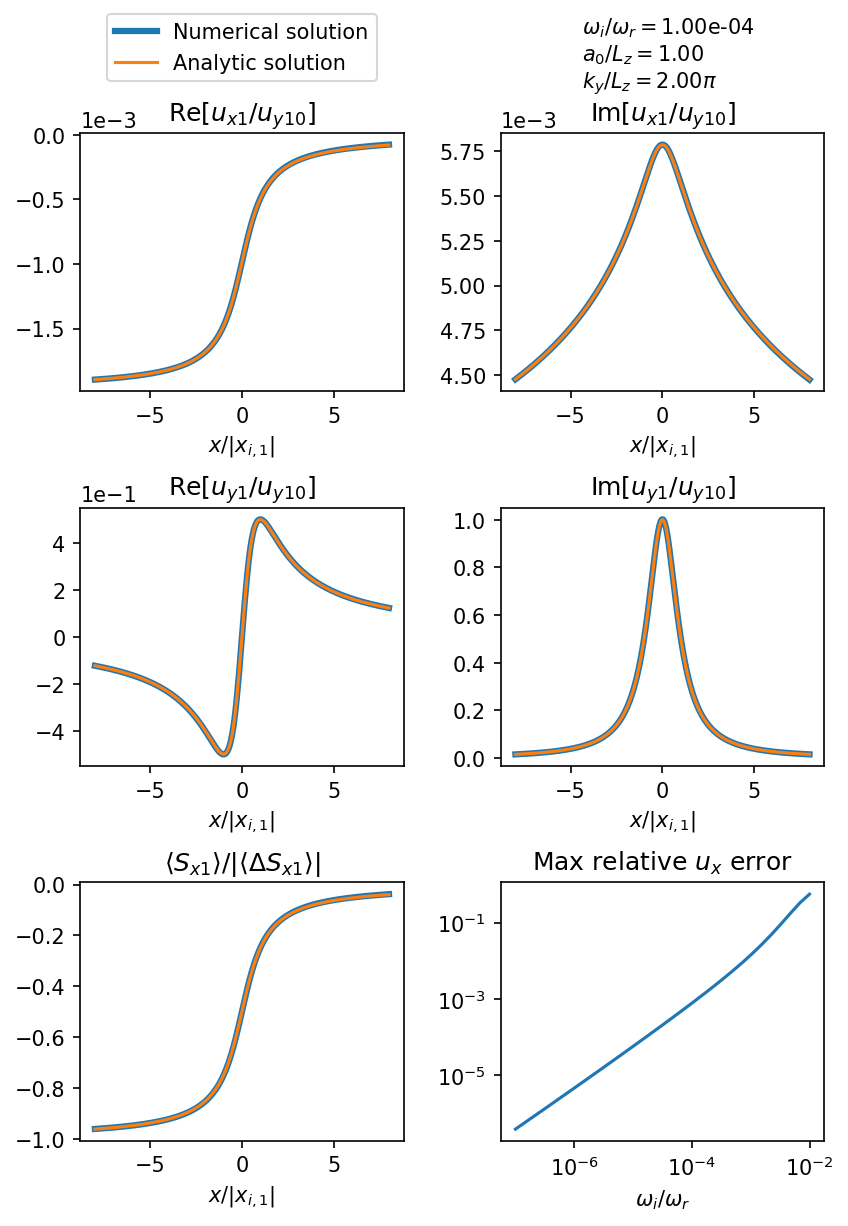
\includegraphics[width=\textwidth,height=0.85\textheight,keepaspectratio]{figures/chapter04/normal_mode_along_x_alpha=0.png}
    \vspace{-10pt}
    \caption{This figure shows the real and imaginary parts of $u_{x1}(x)$, $u_{y1}(x)$, as well as the Poynting flux, $\langle S_{x1}\rangle$ as a function of $x$. The bottom-right shows the maximum relative error between the numerical and analytic solutions for $u_x$ against $\omega_i$ (see Equation \ref{eq:chap_4_max_relative_ux_error}). We calculated the blue curves numerically and calculated the orange curves analytically. Note that the Poynting flux is normalised by the absolute value of the jump, $\abs{\langle\Delta S_{x1}\rangle}$, from Equation \eqref{eq:chap_4_jump_in_poynting_flux}. The code used to make this figure is available on GitHub in the following directory \textcolor{red}{Need to change $u_{y10}$ to $u_0$ and $\ln(x-x_{res,1})$ to $\ln(X_1)$.}:\newline
    \texttt{$\rightarrow$ Python/Chapter4/normal\_mode\_along\_x\_alpha=0.py}}
    \vspace{-20pt}
    \label{fig:normal_mode_along_x_alpha=0}
\end{figure}

To check the accuracy and give a visualisation of Equations \eqref{eq:uxn_leading_order_solution}, \eqref{eq:uyn_leading_order_solution} and \eqref{eq:chap_4_avg_poy_flux_leading_order_alpha=0}, we plot these solutions and compare them with solutions calculated numerically. In the top row of Figure \ref{fig:normal_mode_along_x_alpha=0} we show the real and imaginary parts of $u_{x1}(x)$. The analytic solution was calculated using Equation \eqref{eq:uxn_leading_order_solution}. The blue curve shows the numerical solution and the orange curve shows the analytic solution using Equation \eqref{eq:uxn_leading_order_solution}. The middle row shows the real and imaginary parts of $u_{y1}(x)$. The numerical solution was calculated by rearranging Equation \eqref{eq:chap_4_uy_eqn2_alpha=0}, to give
\begin{equation}
    u_{yn}(x)=\frac{-ik_y}{\mathcal{L}_n(x)-k_y^2}\dv{u_{xn}}{x}.
\end{equation}
The analytic solution was calculated using Equation \eqref{eq:uyn_leading_order_solution}.
The bottom left plot shows the average Poynting flux directed in the $x$-direction. This was calculated using Equation \eqref{eq:chap_4_avg_poy_flux_nth_contribution} for $n=1$. To calculate $\hat{b}_{z1}(x)$ numerically we used Equation \eqref{eq:chap_4_bz_eqn2_alpha=0} to give
\begin{equation}
    \hat{b}_{zn}(x)=\frac{1}{i\omega}\qty[\pdv{u_{xn}}{x}+ik_y u_{y n}].
\end{equation}
The analytic solution was calculated using Equation \eqref{eq:chap_4_avg_poy_flux_leading_order_alpha=0}. 
% The Poynting flux is normalised by a term labelled $\langle S_{x10}\rangle$, which is given by
% \begin{equation}
%     \label{eq:Sx10}
%     \langle S_{x10}\rangle = \pi\frac{B_0^2}{\mu}\frac{u_{y10}^2x_{i,1}^2\omega}{v_A^2(x)a(x)}\,\text{sign}(x_i),
% \end{equation}
% which comes from the coefficient of Equation \eqref{eq:chap_4_jump_in_poynting_flux}.
These plots show that the analytic and numerical solutions are in approximate agreement. However, this is for $\omega_i/\omega_r = 10^{-4}$. In the bottom right, we show the maximum relative error between the analytic and numerical solutions for $u_x$ as a function of $\omega_i$. The maximum relative error is given by
\begin{equation}
    \label{eq:chap_4_max_relative_ux_error}
    \text{Max relative $u_x$ error} = \max_{|x|\le 8|x_{i,1}|} \abs{\frac{u_{x,1}^{(num)} - u_{x,1}^{(ana)}}{u_{x,1}^{(num)}}},
\end{equation}
where $u_{x,1}^{(num)}$ denotes $u_{x,1}$ calculate numerically and $u_{x,1}^{(ana)}$ denotes $u_{x,1}$ calculated analytically using Equation \eqref{eq:uxn_leading_order_solution}. The bottom-right plot shows that as $\omega_i/\omega_r$ increases, there error between the analytic and numerical solutions increases.

\section{Oblique field: Uniform density profile}
\label{sec:oblique_field_uniform_density_profile_with_line_tied_bcs}

This section aims to show how boundary layers can form if the background magnetic field is oblique to the $z=z_{min}$ and $z=z_{max}$ boundaries. For simplicity, we will model the background Alfv\'en speed as uniform, i.e. $v_A(x,z)=v_{A0}$ as this allows us to derive a simple algebraic dispersion relation. We will calculate the normal mode solution in a domain where we impose an incident Alfv\'en wave from $z>0$ and line-tied boundary conditions at $z=0$. Results from this section will be compared with results from Section \ref{sec:oblique_field_piecewise_constant_density_profile} to test the validity of imposing line-tied boundary conditions.

\subsection{Dispersion relation}

Since the background Alfv\'en speed is uniform we can derive a dispersion relation using a method very similar to that used in Section \ref{sec:mhd_waves_dispersion_relation}. The derivation here is almost identical except $\pdv*{}{y}\rightarrow\nabla_\perp$ and $\pdv*{}{z}\rightarrow\nabla_{||}$.
Eliminating $\hat{b}_x$ and $\hat{b}_{||}$ from Equations \eqref{eq:chap_4_ux_eqn1} and \eqref{eq:chap_4_u_perp_eqn1} gives
\begin{gather}
    \qty[\pdv[2]{}{t}-v_{A0}^2\nabla_{||}^2]u_x=-v_{A0}^2\pdv{\hat{b}_{||}}{x}{t}, \\
    \qty[\pdv[2]{}{t}-v_{A0}^2\nabla_{||}^2]u_\perp=-v_{A0}^2\nabla_\perp\pdv{\hat{b}_{||}}{t}.
\end{gather}
Eliminating $\hat{b}_{||}$ gives
\begin{gather}
    \label{eq:chap_4_ux_u_perp_eqn_uniform_in_x}
    \qty[\pdv[2]{}{t}-v_{A0}^2\qty(\pdv[2]{}{x}+\nabla_{||}^2)]u_x=v_A^2(z)\nabla_\perp\pdv{u_\perp}{x}, \\
    \qty[\pdv[2]{}{t}-v_{A0}^2\qty(\nabla_\perp^2+\nabla_{||}^2)]u_\perp=v_A^2(z)\nabla_\perp\pdv{u_x}{x}.
\end{gather}
For $z\ne0$,
\[\qty[\pdv[2]{}{t}-v_{A0}^2\qty(\nabla_\perp^2 + \nabla_{||}^2)]\qty[\pdv[2]{}{t}-v_{A0}^2\qty(\pdv[2]{}{x}+\nabla_{||}^2)]u_\perp=v_A^4\nabla_\perp^2 \pdv[2]{u_\perp}{x},\]
\[\implies \qty[\pdv[2]{}{t}-v_{A0}^2\nabla_{||}^2]\qty[\pdv[2]{}{t}-v_{A0}^2\qty(\pdv[2]{}{x}+\nabla_{||}^2)]u_\perp-v_{A0}^2\nabla_\perp^2\qty[\pdv[2]{}{t}-v_{A0}^2\nabla_{||}^2]u_\perp=0,\]
\begin{equation}
    \label{eq:u_perp_eqn_uniform}
    \implies \qty[\pdv[2]{}{t}-v_{A0}^2\nabla_{||}^2]\qty[\pdv[2]{}{t}-v_{A0}^2\qty(\pdv[2]{}{x}+\nabla_\perp^2+\nabla_{||}^2)]u_\perp=0.
\end{equation}
To derive the dispersion relation, assume $u_\perp$ is of the form
\[u_\perp = u_{\perp n}\exp[i(k_x x + k_y y + k_{zn} z + \omega t)]\]
Substituting this into Equation \eqref{eq:u_perp_eqn_uniform} gives the following dispersion relations
\begin{equation}
    [\omega^2+v_{A0}^2\nabla_{||n}^2][\omega^2-v_{A0}^2(k_x^2+k_y^2+k_{zn}^2)]=0,
\end{equation}
where
\begin{equation}
    \nabla_{||n} = i(k_y\sin\alpha+k_{zn}\cos\alpha).
\end{equation}
Hence, the possible values of $k_{zn}$ are
\begin{equation}
\label{eq:chap_4_oblique_field_uniform_dispersion_relation}
\begin{pmatrix}
k_{z1} \\
k_{z2} \\
k_{z3} \\
k_{z4} \\
\end{pmatrix}
=
\begin{pmatrix}
 \omega / (v_{A0} \cos\alpha) - k_y\tan\alpha \\
-\omega / (v_{A0} \cos\alpha) - k_y\tan\alpha \\
 i\sqrt{k_x^2+k_y^2 - \omega^2/v_{A0}^2} \\
-i\sqrt{k_x^2+k_y^2 - \omega^2/v_{A0}^2}
\end{pmatrix}.
\end{equation}
Where $k_{z1}$, $k_{z2}$ correspond to Alfv\'en wave solutions and $k_{z3}$, $k_{z4}$ correspond to fast wave solutions. Note that the fast wave solutions are evanescent for $k_x^2+k_y^2>\omega^2/v_{A0}^2$.

\subsection{Normal mode solution}

In this section, we will calculate the solution in an infinite domain where we impose an incident Alfv\'en wave from the right ($z>0$) with $\vec{u}=0$ at $z=0$. We assume the solutions are of the form 
\begin{equation}
    \label{eq:chap_4_uniform_density_full_soln}
    \begin{pmatrix}
    u_x \\
    u_\perp \\
    b_x \\
    b_\perp \\
    b_{||}
    \end{pmatrix}
    =\sum_{n=1}^4 \begin{pmatrix}
    u_{xn}\\
    u_{\perp n} \\
    b_{xn} \\
    b_{\perp n} \\
    b_{|| n}
    \end{pmatrix}
    \exp[i(k_x x + k_y y + k_{zn} z + \omega t)],
\end{equation}
where each $k_{zn}$ is given by Equation \eqref{eq:chap_4_oblique_field_uniform_dispersion_relation}.

We impose an incident Alfv\'en wave from the right by setting $u_{\perp1}=u_0$, where $u_0$ gives the incident wave amplitude. We impose the amplitude of the incident fast waves to be zero, therefore, $u_{\perp4}=0$.  From Equation \eqref{eq:chap_4_ux_u_perp_eqn_uniform_in_x} we know that
\begin{equation}
    \begin{aligned}
    u_{x n} &= \frac{-ik_x\nabla_{\perp n}}{\mathcal{L}_{n}-k_x^2}u_{\perp n} \\
    &= \hat{u}_{x n}u_{\perp n},
\end{aligned}
\end{equation}
where
\begin{gather}
    \hat{u}_{x n} = \frac{-ik_x\nabla_{\perp n}}{\mathcal{L}_{n}-k_x^2}, \\
    \mathcal{L}_{n}=\nabla_{||n}^2+\omega^2/v_{A0}^2, \\
    \nabla_{\perp n} = i(k_y\cos\alpha - k_{zn}\sin\alpha), \\
    \nabla_{||n} = i(k_y\sin\alpha+k_{zn}\cos\alpha).
\end{gather}
We require $u_x(x,y,0,t)=u_\perp(x,y,0,t)=0$, hence,
\begin{equation}
\begin{pmatrix}
1 & 1 \\
\hat{u}_{x2} & \hat{u}_{x3}
\end{pmatrix}
\begin{pmatrix}
u_{\perp 2} \\
u_{\perp 3} \\
\end{pmatrix}
=
-u_0
\begin{pmatrix}
1 \\
\hat{u}_{x1}
\end{pmatrix}.
\end{equation}
Hence,
\begin{equation}
    \begin{pmatrix}
    u_{\perp 1} \\
    u_{\perp 2} \\
    u_{\perp 2}
    \end{pmatrix}
    = u_0
    \begin{pmatrix}
    1 \\
    -(\hat{u}_{x1}-\hat{u}_{x3})/(\hat{u}_{x2}-\hat{u}_{x3}) \\
    (\hat{u}_{x1}-\hat{u}_{x2})/(\hat{u}_{x2}-\hat{u}_{x3})
    \end{pmatrix}
\end{equation}
From Equations \eqref{eq:chap_4_bx_eqn1}, \eqref{eq:chap_4_b_perp_eqn1} and \eqref{eq:chap_4_b_par_eqn1}, we know that
\begin{gather}
    \hat{b}_{xn0} = \frac{\nabla_{||n}}{i\omega}u_{xn0}, \\
    \hat{b}_{\perp n0} = \frac{\nabla_{||n}}{i\omega}u_{\perp n0}, \\
    \label{eq:chap_4_uniform_density_b_par0}
    \hat{b}_{|| n0} = -\frac{1}{i\omega}\qty[ik_x u_{xn0}+\nabla_{\perp n} u_{\perp n0}].
\end{gather}

To help visualise the solutions and to check $u_x=u_\perp=0$ at $z=0$ we plot the solutions in Figure \ref{fig:uniform_density_profile}. We choose a large value of $k_x$, namely, $k_x = 50\omega/v_{A0}$, to simulate the conditions near a singularity in a resonant absorption experiment. This means that the fast wave terms are evanescent. The plots show that for $\hat{b}_x$ and $\hat{b}_{||}$ the evanescent fast waves dominate near $z=0$. For $u_x$ and $b_{\perp}$ the evanescent fast waves and Alfv\'en waves are of a similar order near $z=0$. For $u_\perp$, the Alfv\'en waves dominate.

\begin{figure}
    \centering
    \vspace{-20pt}
    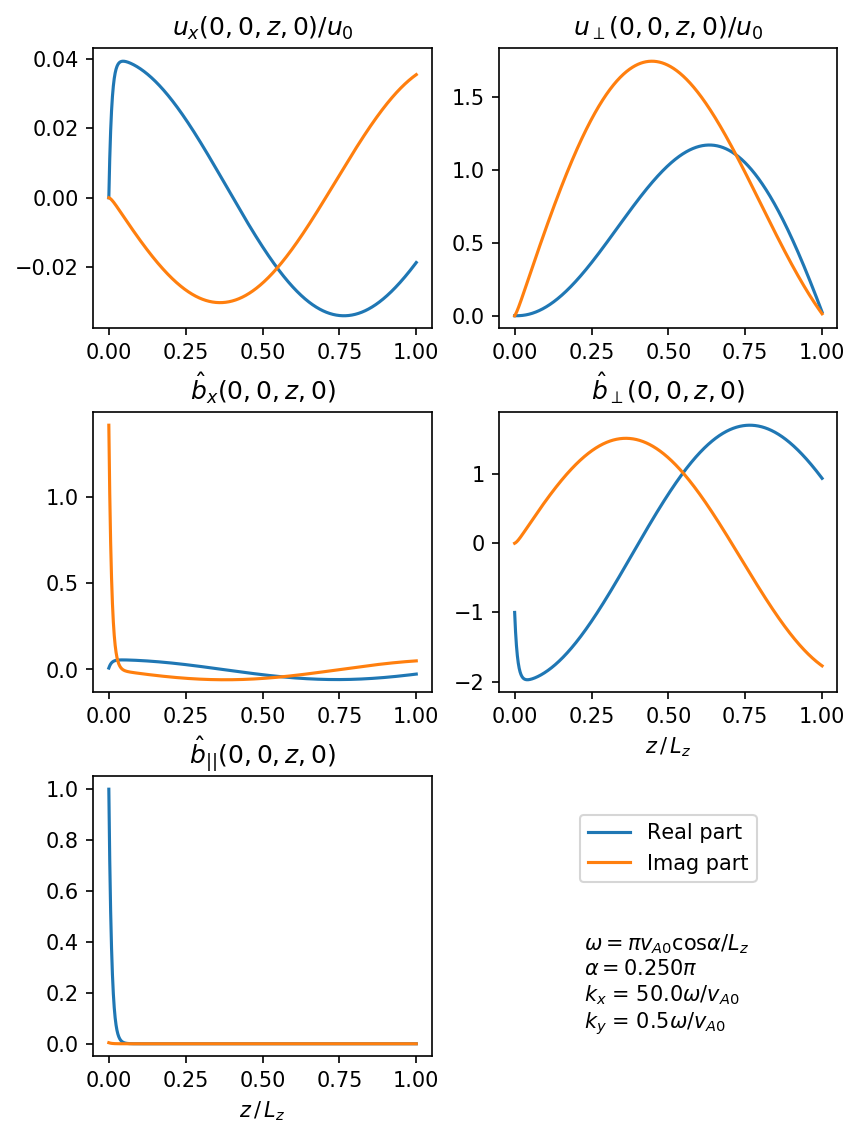
\includegraphics[width=\textwidth,height=0.9\textheight,keepaspectratio]{figures/chapter04/uniform_density_profile.png}
    \vspace{-10pt}
    \caption{This figure shows plots of the real and imaginary parts of $u_x$, $u_\perp$, $b_x$, $b_\perp$ and $b_{||}$ as a function of $z$. We calculated the solutions using Equations \eqref{eq:chap_4_uniform_density_full_soln}-\eqref{eq:chap_4_uniform_density_b_par0}. The code used to make this figure is available on GitHub in the following directory:\newline
    \texttt{$\rightarrow$ Python/Chapter4/uniform\_density\_profile.py}}
    \label{fig:uniform_density_profile}
    \vspace{-20pt}
\end{figure}

In Section \ref{sec:normal_field_resonant_absorption_with_line_tied_bcs}, we showed that resonant absorption produces very short length-scales in $x$. Approaching resonant singularities, the length-scales in $x$ shrink to zero. Therefore, we are interested in the limit $k_x\rightarrow \infty$. Note that for $k_x\rightarrow\infty$ the fast wave solutions are evanescent. To help us understand the effects of line-tied boundary conditions, we will now calculate asymptotic expansions for $u_{xn}$, $u_{\perp n}$, $b_{x n}$, $b_{\perp n}$ and $b_{||n}$. We use the following maple file
\begin{verbatim}
    Maple/Chapter4/uniform_in_x_vA0.mw
\end{verbatim}
on GitHub to calculate the asymptotic expansions. The leading order asymptotic expansion for the $u_x$ coefficients is given by
\begin{gather}
    \label{eq:chap_4_oblique_ux1}
    u_{x1}= -u_0\frac{k_yv_{A0}-\omega\sin\alpha}{v_{A0}\cos\alpha}\frac{1}{k_x} + O\qty(\frac{1}{k_x^2}), \\
    u_{x2}= u_0\frac{k_yv_{A0}+\omega\sin\alpha}{v_{A0}\cos\alpha}\frac{1}{k_x} + O\qty(\frac{1}{k_x^2}), \\
    \label{eq:chap_4_oblique_ux3}
    u_{x3}= -2u_0\tan\alpha\frac{\omega}{v_{A0}}\frac{1}{k_x} + O\qty(\frac{1}{k_x^2}).
\end{gather}
The leading order asymptotic expansion for the $u_\perp$ coefficients is given by
\begin{gather}
    u_{\perp1} = u_0, \\
    u_{\perp2} = -u_0 + O\qty(\frac{1}{k_x}), \\
    u_{\perp3} = 2iu_0\frac{\omega\sin^2\alpha}{v_{A0}\cos\alpha}\frac{1}{k_x} + O\qty(\frac{1}{k_x^2}).
\end{gather}
The leading order asymptotic expansion for the $\hat{b}_x$ coefficients is given by
\begin{gather}
    b_{x1} = -u_0\frac{k_yv_{A0}-\omega\sin\alpha}{v_{A0}^2\cos\alpha}\frac{1}{k_x} + O\qty(\frac{1}{k_x^2}), \\
    b_{x2} = -u_0\frac{k_yv_{A0}+\omega\sin\alpha}{v_{A0}^2\cos\alpha}\frac{1}{k_x} + O\qty(\frac{1}{k_x^2}), \\
    b_{x3} = -2i\frac{u_0}{v_{A0}}\sin\alpha + O\qty(\frac{1}{k_x}).
\end{gather}
The leading order asymptotic expansion for the $\hat{b}_\perp$ coefficients is given by
\begin{gather}
    b_{\perp1} = \frac{u_0}{v_{A0}}, \\
    b_{\perp2} = \frac{u_0}{v_{A0}} + O\qty(\frac{1}{k_x}), \\
    b_{\perp3} = -2\frac{u_0}{v_{A0}}\sin^2\alpha + O\qty(\frac{1}{k_x}).
\end{gather}
Finally, The leading order asymptotic expansion for the $\hat{b}_{||}$ coefficients is given by
\begin{gather}
    b_{||1} = 0, \\
    b_{||2} = 0, \\
    \label{eq:chap_4_oblique_b_par3}
    b_{||3} = \frac{u_0}{v_{A0}}\sin(2\alpha) + O\qty(\frac{1}{k_x}).
\end{gather}
For the Alfv\'en wave terms the associated magnetic pressure, $b_{||}$, equals zero and this was shown in Section \ref{sec:mhd_waves_dispersion_relation}. The above equations show that to leading order the $u_x$ solution does include an evanescent fast wave term and this gives rise to the boundary layers seen in \citet{Halberstadt1993,Halberstadt1995,Arregui2003}. However, the leading order $u_\perp$ solution does not contain any fast wave terms. Note that for $b_x$ the boundary layer term dominates near $z=0$.

We now aim to give a brief explanation for why the boundary layers form. Imposing $\vec{u}=0$ at $z=0$ forces the normal component of the magnetic field, $b_z=0$. For proof, consider the $z$-component of the induction equation,
\[\pdv{b_z}{t}=\vec{\hat{z}}\cdot\curl(\vec{u}\cross\vec{B}_0).\]
Note that the curl in the $z$-direction only depends on derivatives in $x$ and $y$. Since  $\vec{u}=0=$ constant at $z=0$, the $x$ and $y$ derivatives are zero. Therefore, if $b_z$ is initially zero it will remain zero for all time, $\implies b_z=0$. Therefore, at $z=0$,
\[b_z = \cos\alpha\, b_{||} - \sin\alpha\, b_\perp=0,\]
rearranging gives
\[b_{||} = \tan\alpha\, b_\perp.\]
Here, $b_\perp$ gives the magnetic field component of the Alfv\'en wave and $b_{||}$ gives the magnetic pressure component of the fast wave. Hence, for $\alpha\ne0$ if there is a large amplitude Alfv\'en wave then there must also be a large amplitude fast wave (for $\alpha \ne 0$). If $v_A^2(k_x^2+k_y^2)>\omega^2$ then this forces the associated $k_z$ to be imaginary which means the fast wave must be evanescent. This explains why the boundary layers form.

Note that for $k_x\rightarrow\infty$, $k_{z3}\rightarrow ik_x$. Therefore, energy associated with the evanescent fast waves is proportional to $\exp(-2k_x z)$. Note that
\begin{equation}
    \int_0^\infty \exp(-2 k_x z) dz = \frac{1}{2k_x}.
\end{equation}
This shows that the energy of evanescent fast waves $\rightarrow 0$ as $k_x\rightarrow \infty$ for $u_0$ fixed. This suggests that the evanescent fast waves will have a limited affect on the rate of resonant absorption since the energy associated with them does not grow as the length-scales in $x$ get shorter and so they cannot be absorbing energy. Moreover, the boundary layers cannot directly transport energy away as they are evanescent.

\section{Oblique field: Piecewise constant density profile}
\label{sec:oblique_field_piecewise_constant_density_profile}

This section aims to check if the boundary layers produced in Section \ref{sec:oblique_field_uniform_density_profile_with_line_tied_bcs} are physical or fictitious artefacts arising from the use of line-tied boundary conditions. Instead of imposing line-tied boundary conditions we use a piecewise constant density profile in $z$, i.e. the Alfv\'en speed is given by
\begin{equation}
    v_A(z) = \begin{cases}
    v_{A-}, & z < 0 \\
    v_{A+}, & z \ge 0.
    \end{cases}
\end{equation}
Note that the region $z>0$ models the corona and $z<0$ models the chromosphere, therefore, $v_{A+} > v_{A-}$ as the density in the chromosphere is higher. We impose an incident Alfv\'en wave from the region $z>0$ and then calculate the unique solution which ensures continuity of $u_x$, $u_\perp$, $\pdv*{u_x}{z}$, $\pdv*{u_\perp}{z}$ at $z=0$.

We assume the solutions are of the form
\begin{equation}
    \begin{pmatrix}
    u_x \\
    u_\perp \\
    \hat{b}_x \\
    \hat{b}_\perp \\
    \hat{b}_{||}
    \end{pmatrix}
    =
    \sum_{n=1}^{4} \begin{pmatrix}
    u_{xn0-} \\
    u_{\perp n-} \\
    \hat{b}_{xn-} \\
    \hat{b}_{\perp n-} \\
    \hat{b}_{||n-}
    \end{pmatrix}
    \exp[i(k_x x + k_y y + k_{zn-}z + \omega t)],\ \text{for}\ z\le 0,
\end{equation}
and 
\begin{equation}
    \begin{pmatrix}
    u_x \\
    u_\perp \\
    \hat{b}_x \\
    \hat{b}_\perp \\
    \hat{b}_{||}
    \end{pmatrix}
    =
    \sum_{n=1}^{4} \begin{pmatrix}
    u_{xn+} \\
    u_{\perp n+} \\
    \hat{b}_{xn+} \\
    \hat{b}_{\perp n+} \\
    \hat{b}_{||n+}
    \end{pmatrix}
    \exp[i(k_x x + k_y y + k_{zn+}z + \omega t)],\ \text{for}\ z> 0,
\end{equation}
where
\begin{equation}
\begin{pmatrix}
k_{z1\pm} \\
k_{z2\pm} \\
k_{z3\pm} \\
k_{z4\pm} \\
\end{pmatrix}
=
\begin{pmatrix}
 \omega/(v_{A\pm}\cos\alpha) - k_y\tan\alpha \\
-\omega/(v_{A\pm}\cos\alpha) - k_y\tan\alpha \\
 i\sqrt{k_x^2+k_y^2 - \omega^2/v_{A\pm}^2} \\
-i\sqrt{k_x^2+k_y^2 - \omega^2/v_{A\pm}^2}
\end{pmatrix}.
\end{equation}

We impose an incident Alfv\'en wave from $z>0$ by setting $u_{\perp1+}=u_0$, where $u_0$ gives the incident wave amplitude. We impose the amplitude of the incident fast waves to be zero, therefore, $u_{\perp 4+}=0$. There are no incident waves from the left, therefore, $u_{\perp2-}=u_{\perp3-}=0$. From Equation \eqref{eq:chap_4_ux_u_perp_eqn_uniform_in_x} we know that
\begin{equation}
    \begin{aligned}
    u_{x n\pm} &= \frac{-ik_x\nabla_{\perp n\pm}}{\mathcal{L}_{n\pm}-k_x^2}u_{\perp n\pm} \\
    &= \hat{u}_{x n\pm}u_{\perp n0\pm},
\end{aligned}
\end{equation}
where
\begin{gather}
    \hat{u}_{x n\pm} = \frac{-ik_x\nabla_{\perp n\pm}}{\mathcal{L}_{n\pm}-k_x^2}, \\
    \mathcal{L}_{n\pm}=\nabla_{||n\pm}^2+\omega^2/v_{A\pm}^2, \\
    \nabla_{\perp n\pm} = i(k_y\cos\alpha - k_{zn\pm}\sin\alpha),
\end{gather}
We require continuity of $u_x$, $\pdv*{u_x}{z}$, $u_\perp$ and $\pdv*{u_\perp}{z}$ at $z=0$. This gives the following equations
\[\sum_{n\in\{1,4\}}u_{xn0-}=\sum_{n=1}^3u_{xn0+}\implies \sum_{n\in\{1,4\}}\hat{u}_{xn0-}u_{\perp n0-}=\sum_{n=1}^3\hat{u}_{xn0+}u_{\perp n0+},\]
\[\sum_{n\in\{1,4\}}k_{zn-}u_{xn0-}=\sum_{n=1}^3k_{zn+}u_{xn0+}\implies \sum_{n\in\{1,4\}}k_{zn-}\hat{u}_{xn0-}u_{\perp n0-}=\sum_{n=1}^3k_{zn+}\hat{u}_{xn0+}u_{\perp n0+},\]
\[\sum_{n\in\{1,4\}}u_{\perp n0-}=\sum_{n=1}^3u_{\perp n0+},\]
\[\sum_{n\in\{1,4\}}k_{zn-}u_{\perp n0-}=\sum_{n=1}^3k_{zn+}u_{\perp n0+}.\]
Written in matrix form, these become
\[
    \begin{pmatrix}
    \hat{u}_{x10-} & \hat{u}_{x40-} & -\hat{u}_{x20+} & -\hat{u}_{x30+} \\
    k_{z1-}\hat{u}_{x10-} & k_{z4-}\hat{u}_{x40-} & -k_{z2+}\hat{u}_{x20+} & -k_{z3+}\hat{u}_{x30+} \\
    1 & 1 & -1 &-1 \\
    k_{z1-} & k_{z4-} & -k_{z2+} & -k_{z3+}
    \end{pmatrix}
    \begin{pmatrix}
    u_{\perp 10-} \\
    u_{\perp 40-} \\
    u_{\perp 20+} \\
    u_{\perp 30+}
    \end{pmatrix}
    =u_0
    \begin{pmatrix}
    \hat{u}_{x10+} \\
    k_{z1+}\hat{u}_{x10+} \\
    1 \\
    k_{z1+}
    \end{pmatrix}.
\]
We can solve this using symbolic and numerical computing environments e.g. Maple, see Github file:
\begin{verbatim}
  Maple/Chapter4/uniform_in_x.mw
\end{verbatim} 
From Equations \eqref{eq:chap_4_bx_eqn1}, \eqref{eq:chap_4_b_perp_eqn1} and \eqref{eq:chap_4_b_par_eqn1}, we know that
\begin{gather}
    \hat{b}_{xn0\pm} = \frac{\nabla_{||n\pm}}{i\omega}u_{xn0\pm}, \\
    \hat{b}_{\perp n0\pm} = \frac{\nabla_{||n\pm}}{i\omega}u_{\perp n0\pm}, \\
    \hat{b}_{|| n0\pm} = -\frac{1}{i\omega}\qty[ik_x u_{xn0\pm}+\nabla_{\perp n\pm} u_{\perp n0\pm}].
\end{gather}
To help check that solutions to the matrix above do indeed ensure continuity of $u_x$, $\pdv*{u_x}{z}$, $u_\perp$, $\pdv*{u_\perp}{z}$ we plot the velocities and their derivatives as a function of $z$ in Figure \ref{fig:piecewise_constant_density_profile}. Also, to help visualise the solutions we plot the Alfv\'en wave component and fast wave component for $u_x$ separately. Since $k_x^2+k_y^2>\omega^2/v_{A\pm}$, the fast wave component is evanescent.

\begin{figure}
    \centering
    \vspace{-20pt}
    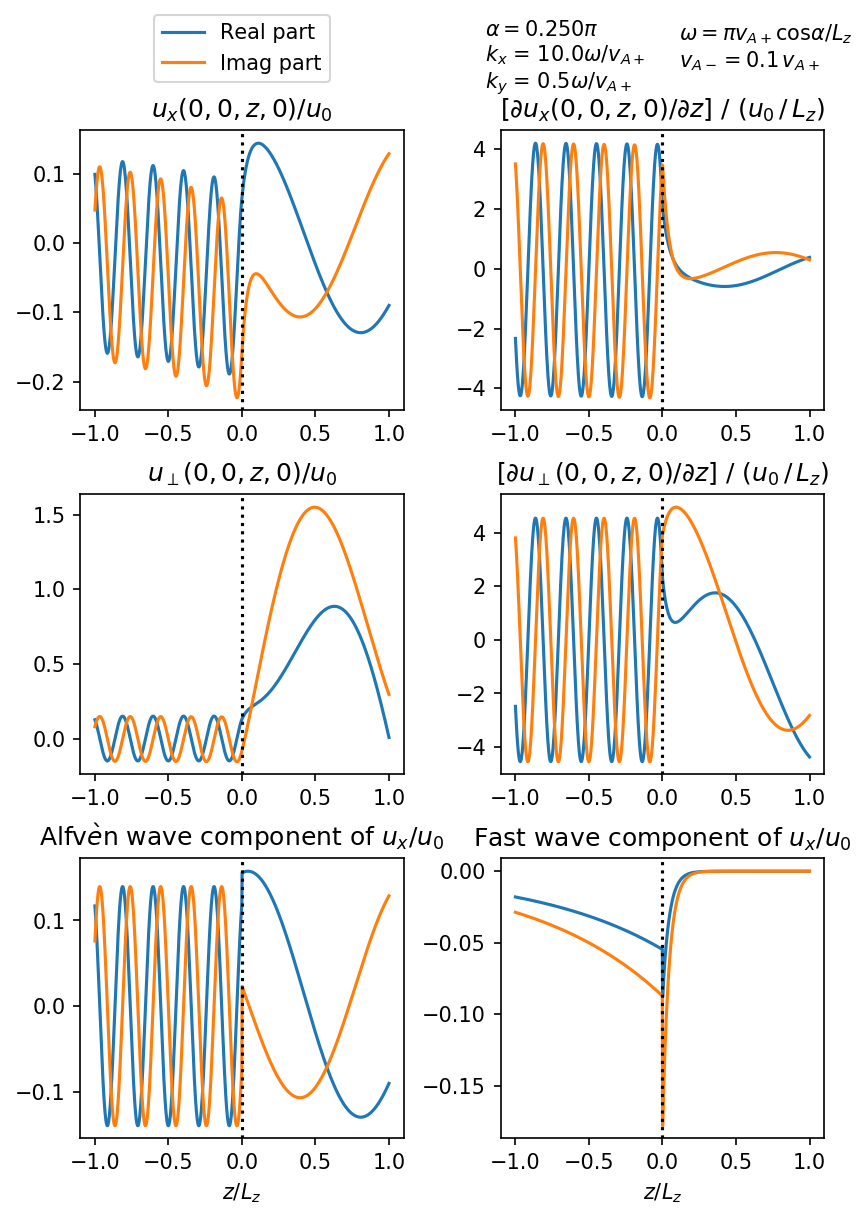
\includegraphics[width=\textwidth,height=0.85\textheight,keepaspectratio]{figures/chapter04/piecewise_constant_density_profile.png}
    \vspace{-10pt}
    \caption{This figure shows plots of the velocity $u_x$, $u_\perp$ and their $z$-derivatives as a function of $z$ at $x=y=t=0$. It shows that the velocities and their $z$-derivatives are continuous. The bottom row shows the Alfv\'en wave and fast components of $u_x$ separately, where the Alfv\'en wave component have wavenumbers $k_{z1\pm}$, $k_{z2\pm}$ and the fast wave component have wavenumbers $k_{z3\pm}$, $k_{z4\pm}$. The code used to make this figure is available on GitHub in the following directory:\newline
    \texttt{$\rightarrow$ Python/Chapter4/piecewise\_constant\_density\_profile.py}}
    \vspace{-20pt}
    \label{fig:piecewise_constant_density_profile}
\end{figure}

Our goal now is to calculate asymptotic expansions for $k_x\rightarrow\infty$ to test if the boundary layers observed in the previous section still form without line-tied boundary conditions. Using the Maple file above we calculate the leading order asymptotic expansions for the $u_x$ coefficients as
\begin{gather}
    \label{eq:oblique_field_uniform_in_x_ux10-}
    u_{x 1-} = -2u_0\frac{k_yv_{A-}-\omega\sin\alpha}{(v_{A+}+v_{A-})\cos\alpha}\frac{1}{k_x} + O\qty(\frac{1}{k_x^2}), \\
    u_{x 4-} = -iu_0\omega^2\frac{(v_{A+}-v_{A-})\sin\alpha}{v_{A+}^2v_{A-}\cos^2\alpha}\frac{1}{k_x^2} + O\qty(\frac{1}{k_x^3}), \\
    u_{x 1+} = -u_0\frac{k_yv_{A+}-\omega\sin\alpha}{v_{A+}\cos\alpha}\frac{1}{k_x} + O\qty(\frac{1}{k_x^2}), \\
    u_{x 2+} = u_0\frac{k_yv_{A+}+\omega\sin\alpha}{v_{A+}\cos\alpha}\frac{v_{A+}-v_{A-}}{v_{A+}+v_{A-}}\frac{1}{k_x} + O\qty(\frac{1}{k_x^2}), \\
    u_{x 3+} = -iu_0\omega^2\frac{(v_{A+}-v_{A-})\sin\alpha}{v_{A+}^2v_{A-}\cos^2\alpha}\frac{1}{k_x^2} + O\qty(\frac{1}{k_x^3}).
\end{gather}
The leading order asymptotic expansions for the $u_\perp$ coefficients are given by
\begin{gather}
    u_{\perp 1-} = \frac{2u_0v_{A-}}{v_{A+}+v_{A-}} + O\qty(\frac{1}{k_x^2}), \\
    u_{\perp 4-} = u_0\omega^2\tan^2\alpha\frac{v_{A+}-v_{A-}}{v_{A+}^2v_{A-}}\frac{1}{k_x^2} + O\qty(\frac{1}{k_x^3}), \\
    u_{\perp 1+} = u_0, \\
    u_{\perp 2+} = -u_0\frac{v_{A+}-v_{A-}}{v_{A+}+v_{A-}} + O\qty(\frac{1}{k_x^2}), \\
    \label{eq:oblique_field_uniform_in_x_u_perp30+}
    u_{\perp 3+} = -u_0\omega^2\tan^2\alpha\frac{v_{A+}-v_{A-}}{v_{A+}^2v_{A-}}\frac{1}{k_x^2} + O\qty(\frac{1}{k_x^3}).
\end{gather}
The leading order asymptotic expansions for the $b_x$ coefficients are given by
\begin{gather}
    \hat{b}_{x 1-} = -2u_0\frac{k_yv_{A-}-\omega\sin\alpha}{v_{A-}(v_{A+}+v_{A-})\cos\alpha}\frac{1}{k_x} + O\qty(\frac{1}{k_x^2}), \\
    \hat{b}_{x 4-} = -u_0\omega\tan\alpha\frac{v_{A+}-v_{A-}}{v_{A+}^2v_{A-}}\frac{1}{k_x} + O\qty(\frac{1}{k_x^2}), \\
    \hat{b}_{x 1+} = -u_0\frac{k_yv_{A+}-\omega\sin\alpha}{v_{A+^2}\cos\alpha}\frac{1}{k_x} + O\qty(\frac{1}{k_x^2}), \\
    \hat{b}_{x 2+} = -u_0\frac{k_y v_{A+} + \omega \sin\alpha}{v_{A+}^2 \cos\alpha}\frac{v_{A+} - v_{A-}}{v_{A+} + v_{A-}}\frac{1}{k_x} + O\qty(\frac{1}{k_x^2}), \\
    \hat{b}_{x 3+} = u_0\omega\tan\alpha\frac{v_{A+}-v_{A-}}{v_{A+}^2v_{A-}}\frac{1}{k_x} + O\qty(\frac{1}{k_x^2}).
\end{gather}
The leading order asymptotic expansions for the $b_\perp$ coefficients are given by
\begin{gather}
    \hat{b}_{\perp 1-} = \frac{2u_0}{v_{A+}+v_{A-}} + O\qty(\frac{1}{k_x^2}), \\
    \hat{b}_{\perp 4-} = -iu_0\omega\frac{\sin^2\alpha}{\cos\alpha}\frac{v_{A+}-v_{A-}}{v_{A+}^2v_{A-}}\frac{1}{k_x} + O\qty(\frac{1}{k_x^2}), \\
    \hat{b}_{\perp 1+} = \frac{u_0}{v_{A+}}, \\
    \hat{b}_{\perp 2+} = \frac{u_0}{v_{A+}}\frac{v_{A+}-v_{A-}}{v_{A+}+v_{A-}} + O\qty(\frac{1}{k_x^2}), \\
    \hat{b}_{\perp 3+} = -iu_0\omega\frac{\sin^2\alpha}{\cos\alpha}\frac{v_{A+}-v_{A-}}{v_{A+}^2v_{A-}}\frac{1}{k_x} + O\qty(\frac{1}{k_x^2}).
\end{gather}
Finally, the leading order asymptotic expansions for the $\hat{b}_{||}$ coefficients are given by
\begin{gather}
    \hat{b}_{|| 1-} = 0, \\
    \hat{b}_{|| 4-} = iu_0\omega\sin\alpha\frac{v_{A+}-v_{A-}}{v_{A+}^2v_{A-}}\frac{1}{k_x} + O\qty(\frac{1}{k_x^2}), \\
    \hat{b}_{|| 1+} = 0, \\
    \hat{b}_{|| 2+} = 0, \\
    \label{eq:oblique_field_uniform_in_x_b_par30+}
    \hat{b}_{|| 3+} = iu_0\omega\sin\alpha\frac{v_{A+}-v_{A-}}{v_{A+}^2v_{A-}}\frac{1}{k_x} + O\qty(\frac{1}{k_x^2}).
\end{gather}
Comparing the leading term in the asymptotic expansion for $u_{\perp40-}$ with $u_0$, we estimate that the velocity amplitude of the fast waves terms is negligible compared with the amplitude of the Alfv\'en wave terms provided
% \[u_0 \gg u_0\omega^2\tan^2\alpha\frac{|v_{A+}-v_{A-}|}{v_{A+}^2v_{A-}}\frac{1}{k_x^2},\]
% \[\implies k_x^2 \gg \omega^2\tan^2\alpha\frac{|v_{A+}-v_{A-}|}{v_{A+}^2v_{A-}},\]
% for $v_{A-}\ll v_{A+}$ this gives
\begin{equation}
    \label{eq:chap_4_kx_condition}
    k_x^2 \gg \frac{\omega^2\tan^2\alpha}{v_{A+}v_{A-}},
\end{equation}
where we assume that $v_{A-}\ll v_{A+}$. Our goal now is to verify if this condition is satisfied for realistic coronal parameters. We can approximate the growth in $k_x$ due to phase mixing by rearranging Equation \eqref{eq:kx_star} to give
\begin{equation}
    \label{eq:kx_growth}
    k_x = \frac{1}{a}\frac{t}{\tau_A},
\end{equation}
where 
\begin{gather}
    \tag{\ref{eq:chap_3_alfven_travel_time}}
    \tau_A = \frac{L}{v_A}, \\
    \tag{\ref{eq:length_scale_alfven_travel_time}}
    a = \frac{v_A}{\dv*{v_A}{x}},
\end{gather}
and $L$ gives the length of the coronal loop. Rearranging Equation \eqref{eq:chap_4_kx_condition} and substituting Equation \eqref{eq:kx_growth}  we require
\begin{equation}
    \begin{aligned}
        1 &\gg \frac{\omega^2 \tan^2\alpha}{v_{A+}v_{A-}k_x^2} \\
         &\approx 10^{-1}\qty(\frac{a}{10^6\si{.m}})^2\qty(\frac{\omega}{10^{-2}\si{.Hz}})^2\qty(\frac{10^6\si{.m.s^{-1}}}{v_{A+}})\qty(\frac{10^3\si{.m.s^{-1}}}{v_{A-}})\tan^2\alpha,
    \end{aligned}
\end{equation}
where we substituted $t=\tau_A$. Note that \citet{Roberts2019} estimates resonant absorption causes waves to decay on a timescale of about 20 Alfv\'en travel times, $\tau_A$. Moreover, this assumes that the waves initially have $k_x=0$, in reality, $k_x$ will usually have some non-zero value before the resonant absorption occurs. The above equation shows that Equation \eqref{eq:chap_4_kx_condition}, is usually satisfied after one Alfv\'en travel time in a typical coronal loop. We use a value of $a=1\si{.Mm}$ because \citet{Klimchuk2015} shows that coronal loops have a characteristic diameter of approximately $1.5\si{.Mm}$. If we assume a density contrast, $\rho_i/\rho_o=2$, \citep{Hood2013,Pascoe2013} where $\rho_i$ gives the density inside a loop and $\rho_o$ gives the density outside a loop then this gives a length-scale $a\approx1\si{.Mm}$.

The asymptotic expansions show that to leading order the velocity does not contain any fast-wave terms. Compare this with the asymptotic expansions (see Equations \ref{eq:oblique_field_uniform_in_x_ux10-}-\ref{eq:oblique_field_uniform_in_x_b_par30+}) from the previous section which showed $u_x$ does contain a fast wave to leading order. This suggests that imposing line-tied boundary conditions can cause the model to overestimate greatly the amplitude of the boundary layers. It also suggests that in a resonant absorption experiment the fast wave terms for $u_x$ and $u_\perp$ should be negligible near the singularities. We verify this claim in the next section. 

\section{Oblique field: Resonant absorption}
\label{sec:oblique_field_resonant_absorption}

In this section, we allow the Alfv\'en speed to be dependent on $x$ as this enables resonant absorption to occur. Our goal in this section is to verify our claim, (see end of Section \ref{sec:oblique_field_piecewise_constant_density_profile}) that the velocity amplitude of the boundary layers should be negligible near the singularity in a resonant absorption experiment.

\subsection{Model and equations}

The Alfv\'en speed is given by $v_A(x,z)=\hat{v}_A(x)v_A(0,z)$, where $v_A(0,z)$ is given by Equation \eqref{eq:chap_4_vA(0,z)} and $\hat{v}_A(x)$ is an arbitrary function of $x$ satisfying $\hat{v}_A(x)=1$. 

We seek normal mode solutions and assume the variables are of the form
\[f(x,y,z,t) = f'(x,z)\exp\{i[k_\perp(\cos\alpha\,y - \sin\alpha\,z)+\omega t]\}.\]
Note that
\[\nabla_\perp f(x,y,z,t) = \exp\{i[k_\perp(\cos\alpha\,y - \sin\alpha\,z)+\omega t]\}\qty(ik_\perp - \sin\alpha\pdv{}{z})f',\]
\[\nabla_{||} f(x,y,z,t) = \exp\{i[k_\perp(\cos\alpha\,y - \sin\alpha\,z)+\omega t]\}\cos\alpha\pdv{f'}{z} .\]
Therefore, Equations \eqref{eq:chap_4_ux_eqn1}-\eqref{eq:chap_4_b_par_eqn1} can be simplified to
\begin{gather}
    i\omega u_x'=v_A^2(x,z)\qty[\nabla_{||}'\hat{b}_x' - \pdv{\hat{b}_{||}'}{x}], \\
    i\omega u_\perp'=v_A^2(x,z)\qty[\nabla_{||}'\hat{b}_\perp'-\nabla_\perp' \hat{b}_{||}'], \\
    i\omega \hat{b}_x'=\nabla_{||}'u_x', \\
    i\omega \hat{b}_\perp'=\nabla_{||}'u_{\perp}', \\
    i\omega \hat{b}_{||}'=-\qty[\pdv{u_x'}{x}+\nabla_\perp' u_{\perp}'].
\end{gather}
where
\begin{gather}
    \nabla_\perp' = \qty(ik_\perp - \sin\alpha\pdv{}{z}), \\
    \nabla_{||}' = \cos\alpha\pdv{}{z}.
\end{gather}
Eliminating $\hat{b}_x'$ and $\hat{b}_\perp'$ gives
\begin{gather}
    \label{eq:chap4_ux_eqn_DAE}
    \pdv{u_x'}{x} = -\qty[i\omega \hat{b}_{||'} + \nabla_\perp' u_\perp'], \\
    \label{eq:chap4_b_par_eqn_DAE}
    \pdv{\hat{b}_{||}'}{x} = -\frac{i}{\omega}\mathcal{L}'u_x', \\
    \label{eq:chap4_u_perp_eqn_DAE}
    \mathcal{L}'u_\perp' = i\omega \nabla_\perp' \hat{b}_{||}',
\end{gather}
% and for $z\ne0$
% \begin{equation}
%     \label{eq:chap4_nabla_perp_u_perp_eqn_DAE}
%     \mathcal{L}'\nabla_\perp' u_\perp' = i\omega \nabla_\perp'^2 \hat{b}_{||}',
% \end{equation}
where
\begin{equation}
    \mathcal{L}' = \nabla_{||}'^2+\frac{\omega^2}{v_A^2(x,z)}.
\end{equation}

Note that the $z$ domain is given by $-L_z\le z\le L_z$. In this section, we impose periodic boundary conditions such that 
\begin{gather}
    \label{eq:chap_4_periodic_bcs}
    u_x'(x,-L_z)=u_x'(x,L_z),\quad \left.\pdv{u_x'}{z}\right|_{z=-L_z}=\left.\pdv{u_x'}{z}\right|_{z=L_z}, \\
    b_{||}'(x,-L_z)=b_{||}'(x,L_z),\quad \left.\pdv{b_{||}'}{z}\right|_{z=-L_z}=\left.\pdv{b_{||}'}{z}\right|_{z=L_z}, \\
    u_\perp'(x,-L_z)=u_\perp'(x,L_z),\quad \left.\pdv{u_\perp'}{z}\right|_{z=-L_z}=\left.\pdv{u_\perp'}{z}\right|_{z=L_z}.
\end{gather}
We choose these boundary conditions because they can be easily implemented both numerically and analytically without introducing fictitious boundary layers. Our model approximates a loop in the corona which goes into the chromosphere then back into the corona and so on.

\subsection{Eigenfunctions and eigenfrequencies}

To help solve Equations \eqref{eq:chap4_ux_eqn_DAE}-\eqref{eq:chap4_u_perp_eqn_DAE} we assume the solutions are of the form
\begin{gather}
    \label{eq:chap_4_oblique_ux_eigenfunction_expansion}
    u_x'(x,z) = u_{x0}^{(1)}(x)\phi_0(z) + \sum_{n=1}^\infty u_{xn}^{(1)}(x)\phi_n(z) + u_{xn}^{(2)}(x)\varphi_n(z), \\
    \label{eq:chap_4_oblique_b_par_eigenfunction_expansion}
    b_{||}'(x,z) = b_{||0}^{(1)}(x)\phi_0(z) + \sum_{n=1}^\infty b_{||n}^{(1)}(x)\phi_n(z) + b_{||n}^{(2)}(x)\varphi_n(z), \\
    \label{eq:chap_4_oblique_u_perp_eigenfunction_expansion}
    u_\perp'(x,z) = u_{\perp0}^{(1)}(x)\phi_0(z) + \sum_{n=1}^\infty u_{\perp n}^{(1)}(x)\phi_n(z) + u_{\perp n}^{(2)}(x)\varphi_n(z),
\end{gather}
where $\phi_n$, $\varphi_n$ are eigenfunctions, with eigenfrequencies, $\omega_n$, $\varpi_n$, respectively. The eigenfunctions satisfy the following Sturm-Liouville equations,
\[\qty[\nabla_{||}'^2+\frac{\omega_n^2}{v_A^2(0,z)}]\phi_n(z)=0,\]
\[\qty[\nabla_{||}'^2+\frac{{\varpi}_n^2}{v_A^2(0,z)}]\varphi_n(z)=0,\]
as well as the periodic boundary conditions, see Equation \eqref{eq:chap_4_periodic_bcs}.

By symmetry, we assume the eigenfunctions are of the form
\begin{gather}
\phi_n(z)=A_n\begin{cases}
a_n\cos[k_{zn-} (z+l_z)], & z < 0, \\
c_n\cos[k_{zn+} (z-l_z)], & z \ge 0, \\
\end{cases} \\
\varphi_n(z)=B_n\begin{cases}
b_n\sin[\bar{k}_{zn-} (z+l_z)], & z < 0, \\
d_n\sin[\bar{k}_{zn+} (z-l_z)], & z \ge 0, \\
\end{cases}
\end{gather}
where $a_n$, $b_n$, $c_n$, $d_n$ are constants, $L_z = 2l_z$ and
\begin{gather}
    k_{zn\pm} = \frac{\omega_n}{v_{A\pm}\cos\alpha}, \\
    \bar{k}_{zn\pm} = \frac{\varpi_n}{v_{A\pm}\cos\alpha}.
\end{gather}
Hence
\begin{gather}
    \dv{\phi_n}{z}=A_n\begin{cases}
    -a_nk_{zn-}\sin[k_{zn-} (z+l_z)], & z < 0, \\
    -c_nk_{zn+}\sin[k_{zn+} (z-l_z)], & z \ge 0, \\
    \end{cases} \\
    \dv{\varphi_n}{z}=B_n\begin{cases}
    b_n\bar{k}_{zn+}\cos[\bar{k}_{zn+} (z+l_z)], & z < 0, \\
    d_n\bar{k}_{zn+}\cos[\bar{k}_{zn+} (z-l_z)], & z \ge 0. \\
    \end{cases}
\end{gather}
We require continuity of $\phi_n$, $\varphi_n$, $\dv*{\phi_n}{z}$, $\dv*{\varphi_n}{z}$ at $z=0$ and $z=\pm L_z$, this gives the following equations
\begin{gather}
\begin{pmatrix}
\cos(k_{zn-}l_z) & -\cos(k_{zn+}l_z) \\
k_{zn-}\sin(k_{zn-}l_z) & k_{zn+}\sin(k_{zn+}l_z)
\end{pmatrix}
\begin{pmatrix}
a_n \\
c_n
\end{pmatrix}
=
\begin{pmatrix}
0 \\
0
\end{pmatrix}, \\
\begin{pmatrix}
\sin(\bar{k}_{zn-}l_z) & \sin(\bar{k}_{zn+}l_z) \\
\bar{k}_{zn-}\cos(\bar{k}_{zn-}l_z) & -\bar{k}_{zn+}\cos(\bar{k}_{zn+}l_z)
\end{pmatrix}
\begin{pmatrix}
b_n \\
d_n
\end{pmatrix}
=
\begin{pmatrix}
0 \\
0
\end{pmatrix}.
\end{gather}
For non-trivial solutions to exist, $\omega_n$, $\varpi_n$ must satisfy
\begin{gather}
\label{eq:omega_n_eqn}
k_{zn+}\sin(k_{zn+}l_z)\cos(k_{zn-}l_z)+k_{zn-}\sin(k_{zn-}l_z)\cos(k_{zn+}l_z)=0, \\
\label{eq:varpi_n_eqn}
\bar{k}_{zn+}\sin(\bar{k}_{zn-}l_z)\cos(\bar{k}_{zn+}l_z)+\bar{k}_{zn-}\sin(\bar{k}_{zn+}l_z)\cos(\bar{k}_{zn-}l_z)=0.
\end{gather}
These equations define, $\omega_n$, $\varpi_n$ and we order them such that
\begin{equation}
    \omega_0<\omega_1<\omega_2...,\quad \varpi_0<\varpi_1<\varpi_2...\,,
\end{equation}
where $\omega_0=\varpi_0=0$.

Note that if $l_z=n\pi/k_{zn+}$ and $l_z=n\pi/\bar{k}_{zn+}$ the above equations simplify to
\[k_{zn-}\sin\qty(n\pi\frac{k_{zn-}}{k_{zn+}})(-1)^n=0,\quad \bar{k}_{zn+}\sin\qty(n\pi\frac{\bar{k}_{zn-}}{\bar{k}_{zn+}})(-1)^n=0,\]
which is satisfied for $v_{A+}/v_{A-}=m$, where $m$ is an integer.
If $l_z=(2n+1)\pi/(2k_{zn+})$ and $l_z=(2n+1)\pi/(2\bar{k}_{zn+})$ the above equations simplify to
\[k_{zn+}(-1)^n\cos\qty(\frac{1}{2}(2n+1)\pi\frac{k_{zn-}}{k_{zn+}})=0,\quad
\bar{k}_{zn-}(-1)^n\cos\qty(\frac{1}{2}(2n+1)\pi\frac{k_{zn-}}{k_{zn+}})=0.\]
which is satisfied for $v_{A+}/v_{A-}=m$, where $m$ is an odd integer. Therefore, for $v_{A+}/v_{A-}=m$, where $m$ is an odd positive integer, a subset of the eigenvalues are given by
\begin{equation}
    \label{eq:eigenfrequencies_for_odd_integer}
    \omega_j=\varpi_j=k\pi\frac{v_{A+}}{L_z}\cos\alpha,
\end{equation}
where $j = [(m-1)/2 + 1]k$ and $k\in\mathds{N}$.

If $\omega_n$, $\varpi_n$ satisfy Equations \eqref{eq:omega_n_eqn} and \eqref{eq:varpi_n_eqn}, then the boundary conditions and continuity conditions are ensured if
\begin{gather}
a_n = \begin{cases}
\cos(k_{zn+} l_z), & \cos(k_{zn+} l_z) \ne 0, \\
k_{zn+}\sin(k_{zn+} l_z), & \cos(k_{zn+} l_z) = 0, \\
\end{cases} \\
c_n = \begin{cases}
\cos(k_{zn-} l_z), & \cos(k_{zn-} l_z) \ne 0, \\
-k_{zn-}\sin(k_{zn-} l_z), & \cos(k_{zn-} l_z) = 0, \\
\end{cases} \\
b_n = \begin{cases}
\sin(\bar{k}_{zn+} l_z), & \sin(\bar{k}_{zn+} l_z) \ne 0, \\
\bar{k}_{zn+}\cos(\bar{k}_{zn+} l_z), & \sin(\bar{k}_{zn+} l_z) = 0, \\
\end{cases} \\
d_n = \begin{cases}
-\sin(\bar{k}_{zn-} l_z), & \sin(\bar{k}_{zn-} l_z) \ne 0, \\
\bar{k}_{zn-}\cos(\bar{k}_{zn-} l_z), & \sin(\bar{k}_{zn-} l_z) = 0. \\
\end{cases}
\end{gather}

Let $\Big\langle f_n(z), f_m(z) \Big\rangle$ denote the following inner product
\begin{equation}
    \Big\langle f_n(z), f_m(z) \Big\rangle = \frac{v_{A+}^2}{L_z}\int_{-L_z}^{L_z} \frac{f_n(z)f_m(z)}{v_A^2(0,z)}dz.
\end{equation}
By Sturm–Liouville theory, the eigenfunctions are orthogonal to each other over this inner product, hence,
\begin{equation}
    \Big\langle \phi_n(z), \varphi_m(z) \Big\rangle = 0.
\end{equation}
We normalise such that
\begin{equation}
    \Big\langle \phi_n(z), \phi_m(z) \Big\rangle = \Big\langle \varphi_n(z), \varphi_m(z) \Big\rangle = \delta_{nm},
\end{equation}
where $\delta_{nm}$ is the Kronecker delta.
Note that
\begin{gather}
    \begin{aligned}
    \frac{L_z}{v_{A+}^2}\frac{\langle \phi_n, \phi_n \rangle}{A_n^2} &= 2\int_{0}^{l_z} \frac{a_n^2}{v_{A-}^2}\cos^2(k_{zn-}z) + \frac{c_n^2}{v_{A+}^2}\cos^2(k_{zn+}z)dz \\
    &=\Bigg\{\frac{a_n^2}{2v_{A-}^2k_{zn-}}\Big[2k_{zn-}z+\sin(2k_{zn-}z)\Big]\\
    &+\frac{c_n^2}{2v_{A+}^2k_{zn+}}\Big[2k_{zn+}z+\sin(2k_{zn+}z)\Big]\Bigg\}_0^{l_z} \\
    &=\frac{a_n^2}{2v_{A-}^2k_{zn-}}\Big[2k_{zn-}l_z+\sin(2k_{zn-}l_z)\Big] \\
    &+\frac{c_n^2}{2v_{A+}^2k_{zn+}}\Big[2k_{zn+}l_z+\sin(2k_{zn+}l_z)\Big],
    \end{aligned} \\
    \begin{aligned}
    \frac{L_z}{v_{A+}^2}\frac{\langle \varphi_n, \varphi_n \rangle}{B_n^2} &=
    \frac{b_n^2}{2v_{A-}^2\bar{k}_{zn-}}\Big[2\bar{k}_{zn-}l_z-\sin(2\bar{k}_{zn-}l_z)\Big]\\
    &+ \frac{b_n^2}{2v_{A-}^2\bar{k}_{zn-}}\Big[2\bar{k}_{zn-}l_z-\sin(2\bar{k}_{zn-}l_z)\Big].
    \end{aligned}
\end{gather}
Hence,
\begin{gather}
    \begin{aligned}
    A_n = \frac{\sqrt{L_z}}{v_{A+}}\Bigg(&\frac{a_n^2}{2v_{A-}^2k_{zn-}}\Big[2k_{zn-}l_z+\sin(2k_{zn-}l_z)\Big] + \\
    &\frac{c_n^2}{2v_{A+}^2k_{zn+}}\Big[2k_{zn+}l_z+\sin(2k_{zn+}l_z)\Big] \Bigg)^{-1/2},
    \end{aligned} \\
    \begin{aligned}
    B_n = \frac{\sqrt{L_z}}{v_{A+}}\Bigg(&\frac{b_n^2}{2v_{A-}^2\bar{k}_{zn-}}\Big[2\bar{k}_{zn-}l_z-\sin(2\bar{k}_{zn-}l_z)\Big] + \\
    & \frac{b_n^2}{2v_{A-}^2\bar{k}_{zn-}}\Big[2\bar{k}_{zn-}l_z-\sin(2\bar{k}_{zn-}l_z)\Big] \Bigg)^{-1/2}.
    \end{aligned}
\end{gather}

\begin{figure}
    \centering
    \vspace{-20pt}
    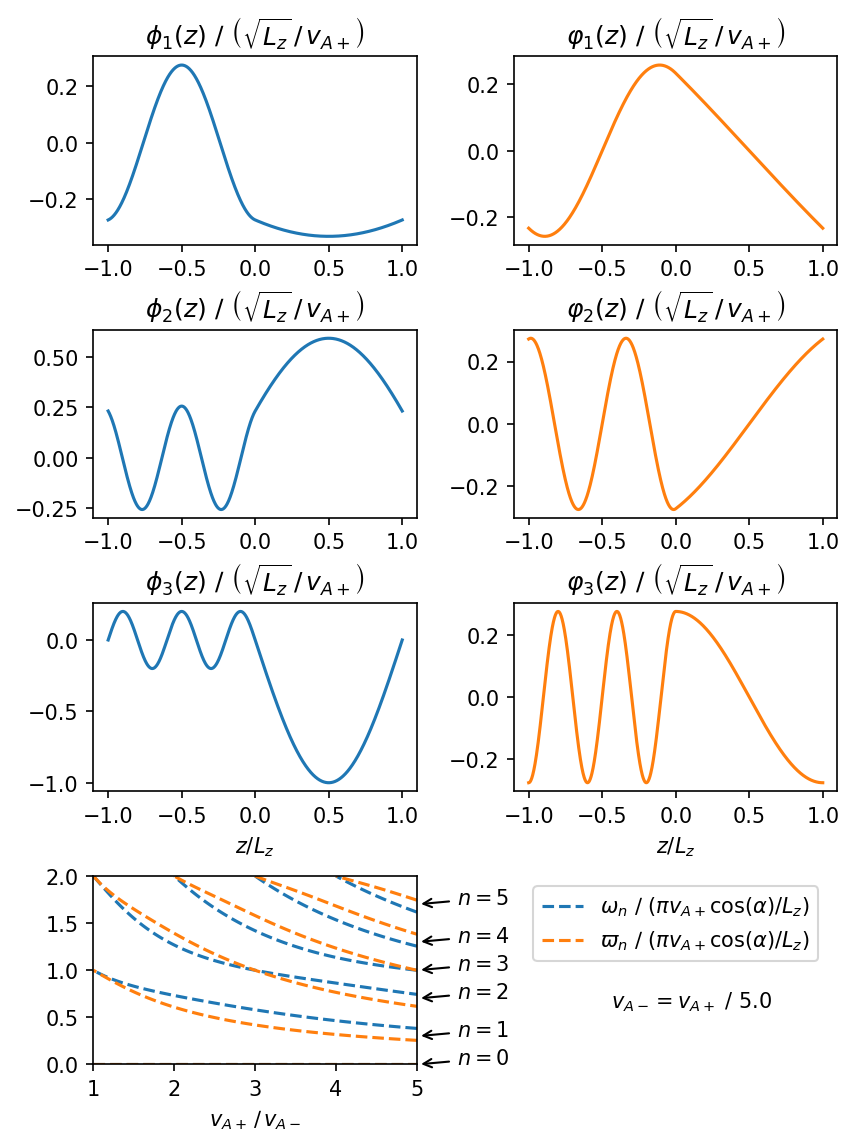
\includegraphics[width=\textwidth,height=0.9\textheight,keepaspectratio]{figures/chapter04/eigenfunctions_and_eigenfrequencies.png}
    \vspace{-10pt}
    \caption{The 1\textsuperscript{st}, 2\textsuperscript{nd} and 3\textsuperscript{rd} rows of this Figure show the 1\textsuperscript{st}, 2\textsuperscript{nd} and 3\textsuperscript{rd} eigenfunctions, $\phi_n(z)$, $\varphi_n(z)$, respectively, where $v_{A-}=v_{A+}/5$. In the bottom-left plot we show the first 5 eigenfrequencies, $\omega_n$, $\varpi_n$ as a function of $v_{A+} / v_{A-}$. \textcolor{red}{Need to remove the normalising constants.} The code we used to make this figure is available on GitHub in the following directory:\newline
    \texttt{$\rightarrow$ Python/Chapter4/eigenfunction\_eigenfrequency\_plots.py}}
    \vspace{-20pt}
    \label{fig:eigenfunctions_and_eigenfrequencies}
\end{figure}

To help visualise the eigenfunctions, we plot the first 3 normalised eigenfunctions (excluding the 0\textsuperscript{th} eigenfunction) in Figure \ref{fig:eigenfunctions_and_eigenfrequencies} for $v_{A-}=v_{A+}/5$. They show that the amplitude of the eigenfunctions in the chromosphere can be as large as the amplitude in the corona, although it never exceeds the coronal amplitudes. The bottom-left of Figure \ref{fig:eigenfunctions_and_eigenfrequencies} shows the first 5 eigenfrequencies as a function of $1/v_{A-}$. They show that decreasing $v_{A-}$ causes $\omega_n$ and $\varpi_n$ to decrease because this lowers the Alfv\'en travel time of the loop. This plot can also be used to check that for $v_{A+}/v_{A-}=m$, where $m$ is an odd integer, a subset of the eigenfrequencies are given by Equation \eqref{eq:eigenfrequencies_for_odd_integer}.

\subsection{Analytic resonant solution}
\label{sec:oblique_field_resonant_absorption_analytic_soln}

\subsubsection{Deriving a PDE for $u_\perp(x,z)$}

Our goal now is to calculate the leading order resonant/singular solution analytically. We will verify our result numerically in the next section. Eliminating $\hat{b}_{||}'$ from Equations \eqref{eq:chap4_ux_eqn_DAE}-\eqref{eq:chap4_u_perp_eqn_DAE} gives
\begin{gather}
    \label{eq:chap_4_ux_eqn_oblique1}
    \qty[\mathcal{L}'+\pdv[2]{}{x}]u_x'=-\pdv{}{x}\nabla_\perp' u_\perp', \\
    \label{eq:chap_4_u_perp_eqn_oblique1}
    [\mathcal{L}'+\nabla_\perp'^2]u_\perp'=-\pdv{}{x}\nabla_\perp' u_x' 
\end{gather}
% We can eliminate $u_\perp'$ with the following procedure. Take the $x$-derivative of Equation \eqref{eq:chap_4_u_perp_eqn_oblique1} and multiply through by $-1$ to give
% \[-\mathcal{L}_x'u_\perp'-[\mathcal{L}'+\nabla_\perp'^2]\pdv{u_\perp'}{x} = \pdv[2]{}{x}\nabla_\perp' u_x'.\]
% Applying $[\mathcal{L}'+\nabla_\perp'^2]\nabla_\perp'$ to both sides and assuming $z\ne-L_z,0,L_z$ gives
% \[-\mathcal{L}_x'\nabla_\perp'[\mathcal{L}'+\nabla_\perp'^2]u_\perp'-[\mathcal{L}'+\nabla_\perp^2]^2\nabla_\perp'\pdv{u_\perp'}{x} = [\mathcal{L}'+\nabla_\perp'^2]\nabla_\perp'^2\pdv[2]{u_x'}{x} .\]
% Eliminating $u_\perp'$ using Equations \eqref{eq:chap_4_ux_eqn_oblique1} and \eqref{eq:chap_4_u_perp_eqn_oblique1} gives
% \[\mathcal{L}_x'\nabla_\perp'^2\pdv{u_x'}{x}+[\mathcal{L}'+\nabla_\perp'^2]^2\qty[\mathcal{L}'+\pdv[2]{}{x}]u_x'=[\mathcal{L}'+\nabla_\perp'^2]\nabla_\perp'^2\pdv[2]{u_x'}{x}.\]
% Rearranging gives
% \begin{equation}
%     \mathcal{L}'[\mathcal{L}'+\nabla_\perp'^2]\pdv[2]{u_x'}{x}+\mathcal{L}_x'\nabla_\perp'^2\pdv{u_x'}{x} + \mathcal{L}'[\mathcal{L}'+\nabla_\perp'^2]^2u_x'=0.
% \end{equation}
We can eliminate $u_x'$ with the following procedure. 
Take the $x$-derivative of the Equation \eqref{eq:chap_4_ux_eqn_oblique1}
\[\mathcal{L}_x'u_x'+\qty[\mathcal{L}'+\pdv[2]{}{x}]\pdv{u_x'}{x}=-\nabla_\perp\pdv[2]{u_\perp'}{x},\]
\[\implies u_x'=-\frac{1}{\mathcal{L}_x'}\qty{\qty[\mathcal{L'}+\pdv[2]{}{x}]\pdv{u_x'}{x}+\nabla_\perp'\pdv[2]{u_\perp'}{x}}.\]
where
\begin{equation}
    \mathcal{L}_x' = \pdv{\mathcal{L}'}{x}=\frac{-2\omega^2}{a(x)v_A^2(x,z)}.
\end{equation}
Substitute this into Equation \eqref{eq:chap_4_ux_eqn_oblique1} to give
\[-\frac{\mathcal{L}'}{\mathcal{L}_x'}\qty{\qty[\mathcal{L}'+\pdv[2]{}{x}]\pdv{u_x'}{x}+\nabla_\perp'\pdv[2]{u_\perp'}{x}}+\pdv[2]{u_x'}{x}=-\nabla_\perp'\pdv{u_\perp'}{x},\]
Applying $-\nabla_\perp'$ to both sides, substituting for $u_x'$ and assuming $z\ne0,-L_z,L_z$ gives
\[-\frac{\mathcal{L}'}{\mathcal{L}_x'}\qty{\qty[\mathcal{L}'+\pdv[2]{}{x}][\mathcal{L}'+\nabla_\perp'^2]u_\perp'-\nabla_\perp'^2\pdv[2]{u_\perp'}{x}}+\pdv{}{x}[\mathcal{L}'+\nabla_\perp'^2]u_\perp'=\nabla_\perp'^2\pdv{u_\perp'}{x}.\]
This can be simplified to give
\begin{equation}
    \label{eq:chap_4_oblique_u_perp_eqn_normal_mode}
     \mathcal{L}'^2\pdv[2]{u_\perp'}{x}+'\mathcal{L}_x'\mathcal{L}'\pdv{u_\perp'}{x}+\mathcal{M}'u_\perp'=0,
\end{equation}
where
\begin{equation}
    \mathcal{M}' = \mathcal{L}'^3+\mathcal{L}'^2\nabla_\perp'^2+\mathcal{L}_{xx}'\mathcal{L}'-\mathcal{L}_x'^2
\end{equation}
From the literature (e.g. \citealt{Thompson1993,Wright1996}) and Section \ref{sec:normal_field_resonant_absorption_with_line_tied_bcs}, we know that resonant absorption can generate singularities in $x$. Equation \eqref{eq:chap_4_oblique_u_perp_eqn_normal_mode} shows that the coefficient of the leading order $x$-derivative goes to zero if $\mathcal{L}'(x,z)=0$. Let
\[x_{res,m} = x_{r,m} + i x_{i,m},\]
be defined as a location which satisfies
\begin{equation}
    \label{eq:x_res_defn}
    \mathcal{L}'(x_{res,m},z)\phi_m(z)=0.
\end{equation}
We postulate that singularities can form at locations, $x_{res,m}$, which are locations where a resonance can occur.

\subsubsection{Deriving an ODE for $u_{\perp m}^{(1)}(x)$}

Our goal now is to convert this PDE into an ODE for $u_{\perp m}^{(1)}(x)$ using the expansion given by Equation \eqref{eq:chap_4_oblique_u_perp_eigenfunction_expansion}. Note that
\[\begin{aligned}
\mathcal{L}'(x,z)\phi_n(z) &= [\omega^2/\hat{v}_A^2(x) - \omega_n^2]\frac{\phi_n(z)}{v_A^2(0,z)} = 0 \\
&= \qty[\mathcal{L}_x'(x_{res,m},z)(x-x_{res,m}) + \frac{1}{2}\mathcal{L}_{xx}'(x_{res,m},z)(x-x_{res,m})^2 + ...]\phi_n(z)\,.
\end{aligned}
\]
Multiplying Equation \eqref{eq:chap_4_oblique_u_perp_eigenfunction_expansion} thorough by $\kappa_m^2(x,z)\phi_mv_{A+}^2/[L_zv_A^2(0,z)]$ where
\begin{equation}
\begin{aligned}
    \kappa_m(x,z) &= (x-x_{res,m})\frac{v_A^2(0,z)}{\omega^2/\hat{v}_A^2(x) - \omega_m^2} \\
    &= (x-x_{res,m})\qty[\mathcal{L}_x'(x_{res,m},z)(x-x_{res,m}) + \frac{1}{2}\mathcal{L}_{xx}'(x_{res,m},z)(x-x_{res,m})^2 + ...]^{-1} \\
    &= \frac{1}{\mathcal{L}_x'(x_{res,m},z)}\qty[1 - \frac{1}{2}\frac{\mathcal{L}_{xx}'(x_{res,m},z)}{\mathcal{L}_x'(x_{res,m},z)}(x-x_{res,m}) + ...], \\
\end{aligned}
\end{equation}
and integrating from $-L_z$ to $L_z$ gives
\begin{equation}
    \label{eq:u_perpm_1_ode1}
    (x-x_{res,m})^2\dv[2]{u_{\perp m}^{(1)}}{x}+(x-x_{res,m})p_m(x)\dv{u_{\perp m}^{(1)}}{x}+q_m(x)u_{\perp m}^{(1)}(x) = f_m(x),
\end{equation}
where
\begin{gather}
    % \begin{aligned}
    % p_m(x) &= \frac{\mathcal{L}_x'v_A^2(0,z)}{\omega^2/\hat{v}_A^2(x)-\omega_m^2}(x-x_{res,m}) \\
    % &= \frac{-2\omega^2/\hat{v}^2_A(x)}{\omega^2/\hat{v}_A^2(x)-\omega_m^2}\frac{x-x_{res,m}}{a(x)},
    % \end{aligned} \\
    p_m(x) = \mathcal{L}_x'(x,z)\kappa_m(x,z), \\
    q_m(x) = \left\langle\mathcal{M}'\phi_m(z), \kappa_m^2(x,z)\phi_m(z)\right\rangle, \\
    \begin{aligned}
    f_m(x) &= -\left\langle\mathcal{M}'u_{\perp m}^{(2)}(x)\varphi_m(z), \kappa_m^2(x,z)\phi_m(z) \right\rangle \\
    &-\sum_{\substack{n=0 \\ n\ne m}}^\infty \left\langle\mathcal{M}'\qty[u_{\perp n}^{(1)}(x)\phi_n(z) + u_{\perp n}^{(2)}(x)\varphi_n(z)],\kappa_m^2(x,z)\phi_m(z)\right\rangle.
    \end{aligned}
\end{gather}

\subsubsection{Complementary function and particular integral}

To solve Equation \eqref{eq:u_perpm_1_ode1} we will first calculate the complementary function by solving the homogeneous equation given by
\begin{equation}
    \label{eq:u_perpm_1_ode_homogenous}
    (x-x_{res,m})^2\dv[2]{u_{\perp m}^{(1)}}{x}+(x-x_{res,m})p_m(x)\dv{u_{\perp m}^{(1)}}{x}+q_m(x)u_{\perp m}^{(1)}(x) = 0.
\end{equation}
We can solve this equation by using the method of Frobenius. We first need to calculate the indicial equation by assuming the solutions are of the form
\[u_{\perp m}^{(1)}(x) = (x-x_{res,m})^\sigma\sum_{n=0}^\infty a_n(x-x_{res,m})^n,\]
to give
\[\sum_{n=0}^\infty a_n[\sigma(\sigma-1)+\sigma p_m(x) + q_m(x)](x-x_{res,m})^{n+\sigma}.\]
Hence, the indicial equation is given by
\begin{equation}
    I(\sigma) = \sigma(\sigma-1) + p_m(x_{res,m})\sigma + q_m(x_{res,m}).
\end{equation}
For non-trivial solution to exist we require $I(\sigma)=0$. Since $p_m(x_{res,m})=-q_m(x_{res,m})=1$ we know that $\sigma =\pm1$. Note that the allowed values of $\sigma$ differ by an integer. Therefore, the general complementary solution for $u_{\perp m}^{(1)}(x)$ is given by a linear combination of
\begin{equation}
    u_{\perp m 1}^{(1)}(x) = \sum_{n=1}^\infty a_n (x-x_{res,m})^n,
\end{equation}
and
\begin{equation}
    u_{\perp m 2}^{(1)}(x) = Cu_{\perp m 1}^{(1)}(x) \ln(x-x_{res,m})+ \sum_{n=-1}^\infty b_n(x-x_{res,m})^n,
\end{equation}
where $a_n$, $b_n$, $C$ are constants.

If we know the power series in $x$ for $f_m(x)$ then we can calculate the particular integral to Equation \eqref{eq:u_perpm_1_ode1} by using the method of undetermined coefficients. Since $f_m(x)$ is proportional to $u_{\perp n}^{(1)}(x)$, $u_{\perp n}^{(2)}(x)$, we know that the leading order term can be at most order $(x-x_{res,m})^{-1}$.

% \subsubsection{Calculating $b_0$}

% Substituting $u_{\perp m 2}^{(1)}(x)$ into Equation \eqref{eq:u_perpm_1_ode_homogenous}, we see that $b_{-1}$ can be arbitrary and from the coefficient of $(x-x_{res,n})^0$ we get
% \[q_m(x_{res,n})b_0 + [q_m'(x_{res,n})-p_m'(x_{res,n})]b_{-1}=0,\]
% where
% % \begin{gather}
% %     p_m'(x_{res,m}) = -\frac{2+a'(x_{res,m})}{2a(x_{res,m})}, \\
% %     \begin{aligned}
% %     q_m'(x_{res,m}) &= -\mathcal{L}_x'(x_{res,m},z)\mathcal{L}_{xx}'(x_{res,m},z)\kappa_m{x_{res,m},z} \\
% %     &=
% %     \end{aligned}
% % \end{gather}
% \begin{gather}
%     \begin{aligned}
%     p_m'(x_{res,m}) &= \dv{}{x}\qty[\mathcal{L}_x'\kappa_m]_{x=x_{res,m}} \\
%     &=  \dv{}{x}\Bigg\{\qty[\mathcal{L}_x'(x_{res,m},z) + \mathcal{L}_{xx}'(x_{res,m},z)(x-x_{res,m})+...] \times\\
%     &\frac{1}{\mathcal{L}_x'(x_{res,m},z)}\qty[1-\frac{1}{2}\frac{\mathcal{L}_{xx}'(x_{res,m},z)}{\mathcal{L}_x'(x_{res,m},z)}(x-x_{res,m})+...]\Bigg\}_{x=x_{res,m}} \\
%     &= \frac{1}{2}\frac{\mathcal{L}_{xx}'(x_{res,m},z)}{\mathcal{L}_x'(x_{res,m},z)}
%     \end{aligned} \\
%     \begin{aligned}
%     q_m'(x_{res,m}) &= \dv{}{x}\qty[(\mathcal{L}_{xx}'\mathcal{L}'-\mathcal{L}_x'^2)\kappa_m^2]_{x=x_{res,m}} \\
%     &=
%     \end{aligned}
% \end{gather}

\subsubsection{Singular solution}

Our goal  now is to calculate a leading order singular solution for $u_x'$, $u_\perp'$ and $\hat{b}_{||}'$ which we can verify numerically.
Assume that $x_{i,m}\ll R$ where $R$ is the radius of convergence of for the power series solution of $u_\perp'(x,z)$ in $x$. We will assume that to leading order $u_{\perp n}^{(1)}=u_{\perp n}^{(2)}=u_{\perp m}^{(2)}=0$ for all $n\ne m$. This ensures that the leading order solution for $u_{\perp m}(x)$ is given by the leading term of the complementary solution. Let $u_\perp'$ be given by
\begin{equation}
    \label{eq:chap_4_oblique_u_perp_final}
    u_\perp'(x,z) = u_0\qty[\frac{\phi_m(z)}{X_{m}} + O(X_m\ln X_m,X_m)],
\end{equation}
where
\begin{equation}
    X_m=\frac{x - x_{res,m}}{x_{i,m}},
\end{equation}
and we choose the boundary conditions such that the terms of order $X_m^0$ equal zero.

% We will assume that we choose 
% We will assume that
% \begin{equation}
%     u_{\perp m}^{(1)}(x) = u_0\qty[X_m +  \hat{u}_{\perp m 0}^{(1)} + O\qty(X_m\ln X_m, X_m)],
% \end{equation}
% and
% \begin{gather}
%     u_{\perp n}^{(1)}(x) = u_0\qty[\hat{u}_{\perp n 0}^{(1)} + O\qty(X_m\ln X_m, X_m)], \\
%     u_{\perp n}^{(2)}(x) = u_0\qty[\hat{u}_{\perp n 0}^{(2)} + O\qty(X_m\ln X_m, X_m)],
% \end{gather}
% for $n\ne m$, where
% \begin{equation}
%     X_m = \frac{x_{i,m}}{x-x_{res,m}},
% \end{equation}
% and we assume that $x_{i,m}<R$, where $R$ is the radius of convergence for the power series solution of $u_\perp$ about $x=x_{res,m}$.

% We assume that $u_\perp'$ is given by Equation \eqref{eq:chap_4_oblique_u_perp_eigenfunction_expansion}. Let $\omega = \omega_r + i \omega_i$, where $\omega_r$ is equal to one of the eigenfrequencies, e.g. $\omega_r = \omega_n$ and $\omega_i \ll \omega_r$. Since the driver frequency, $\omega$, is very close to one of the Alfv\'en wave natural frequencies, $\omega_n$, we expect a resonance to be excited with a singularity at $x=x_{res,n}$, where $x_{res,n}$ satisfies $\mathcal{L}'(x_{res,n},z)\phi_n(z)=0$. Note that
% \[\mathcal{L}'(x_{res},z)\phi_n(z) = [\omega^2/\hat{v}_A^2(x_{res,n}) - \omega_n^2]\frac{\phi_n(z)}{v_A^2(0,z)} = 0,\]
% \[\implies \omega^2= \hat{v}_A^2(x_{res,n}) \omega_n^2.\]
% Let $x_{res,n}=x_{r,n}+ix_{i,n}$, hence,
% \[\omega_r^2 + 2i\omega_r \omega_i \approx \qty(\hat{v}_A^2(x_{r,n})+2ix_{i,n}\frac{\hat{v}_A^2(x_{r,n})}{a(x_{r,n})})\omega_n^2.\]
% Taking the real part gives
% \[\omega_r^2 = \hat{v}_A^2(x_{r,n}) \omega_n^2,\]
% since $\omega_r=\omega_n$, this implies that $x_{r,n}=0$. Taking the imaginary part gives
% \[2\omega_r \omega_i = 2x_{i,n}\frac{\hat{v}_A^2(x_{r,n})}{a(x_{r,n})}\omega_n^2,\]
% hence,
% \begin{equation}
%     x_{i,n} = a(0)\frac{\omega_i}{\omega_n}.
% \end{equation}
% Therefore, 
% \begin{equation}
%     \mathcal{L}'(x_{res},z)\phi_n(z) \approx (x-ix_{i,n})\mathcal{L}_x'(0,z)
% \end{equation}
% gives the leading order Taylor expansion. We are interested in the solution near $x=0$, where $u_{\perp n}^{(1)}(x)$ dominates. Change $x$ to the dimensionless scaled variable 
% \begin{equation}
%     X = \frac{x}{x_{i,n}}.
% \end{equation}
% Substituting $u_{\perp}'(x,z)=u_{\perp n}^{(1)}(x_{i,n}X)\phi_n(z)$ into Equation \eqref{eq:chap_4_oblique_u_perp_eqn_normal_mode} gives
% \begin{equation}
%     (X-i)^2\dv[2]{u_{\perp n}^{(1)}}{X}+(X-i)\dv{u_{\perp n}^{(1)}}{X}- u_{\perp n}^{(1)}= O(x_{i,n}).
% \end{equation}
% Therefore, to leading order, the solution is given by
% \begin{equation}
%     \label{eq:chap_4_oblique_u_perp_final}
%     u_\perp'(x,z) = \frac{u_0 x_{i,n}}{x-ix_{i,n}}\phi_n(z),
% \end{equation}
% where $u_0$ is an arbitrary constant. 

From Equation \eqref{eq:chap_4_u_perp_eqn_oblique1} we know that $u_x$ is given by
\begin{equation}
    \label{eq:chap_4_oblique_ux_final}
    u_x'(x,z) = -u_0\qty[x_{i,m}\ln(X_m)\nabla_\perp'\phi_,(z) + O(X_m,X_m^2\ln X_m)],
\end{equation}
where we impose the boundary condition that terms of order $X_m^0$ equal zero.
From Equation \eqref{eq:chap4_u_perp_eqn_DAE}, we know that to leading order $\hat{b}_{||}'$ satisfies
\begin{equation}
    \label{eq:chap_4_oblique_b_par_final}
    \begin{aligned}
   \nabla_\perp' \hat{b}_{||}'(z) &= u_0\frac{\mathcal{L}_x'(x_{r,m},z)x_{i,m}}{i\omega_r}\phi_m(z) + \frac{O(X_m\ln X_m, X_m)}{L_z} \\
   &= 2iu_0\frac{\omega_r x_{i,m}}{a(x_{r,m})v_A^2(x_{r,m},z)}\phi_m(z) + \frac{O(X_m\ln X_m, X_m)}{L_z},
   \end{aligned}
\end{equation}
assuming $\omega_i\ll\omega_r$
Our goal now is to solve Equation \eqref{eq:chap_4_oblique_b_par_final} for $\hat{b}_{||}'$. For $\sin\alpha=0$, $\hat{b}_{||}'$ is given by
\begin{equation}
    \hat{b}_{||}'(x,z) = \frac{2u_0\omega_r x_{i,m}}{a(x_{r,m})v_A^2(x_{r,m},z)k_\perp}\phi_m(z) + O(X_m\ln X_m, X_m).
\end{equation}
For $\sin\alpha\ne0$, we can calculate $b_{||}'(x,z)$ by using an integrating factor. However, if $k_\perp L_z / \sin\alpha = j\pi$ for $j\in\mathds{Z}$ then $\hat{b}_{||}'(x,z)$ is not uniquely defined by the boundary conditions in $z$. To see this, assume $\hat{b}_{||}(x,z)$ is of the form
\[\hat{b}_{||}'(x,z) = \sum_{n=-\infty}^\infty \hat{b}_{||n}(x)\exp(in\frac{\pi}{L_z}z),\]
This ensures that $\hat{b}_{||}(x,z)$ is periodic in $z$ with period $2L_z$. Substituting this into Equation \eqref{eq:chap_4_oblique_b_par_final}, multiplying by 
$\exp(ij\pi z / L_z) / (2 L_z)$ and integrating from $-L_z$ to $L_z$ gives
\[i\qty(k_\perp - \sin\alpha\, j\frac{\pi}{L_z})\hat{b}_{|| j}(x) = \frac{1}{2L_z}\int_{-L_z}^{L_z}\hat{b}_{||}'(x,z)\exp(ij\frac{\pi}{L_z}z)dz.\]
Hence, if $k_\perp L_z / \sin\alpha = j\pi$ for $j\in\mathds{Z}$ then $\hat{b}_{||j}'(x)$ and consequently $\hat{b}_{||}'(x,z)$ is not uniquely defined by the boundary conditions in $z$. 

% Equation \eqref{eq:chap_4_oblique_b_par_final} can be rearranged to give
% \[\dv{\hat{b}_{||}'}{z} - \frac{ik_\perp}{\sin\alpha}\hat{b}_{||}'(z) = \frac{-2iu_0\omega x_{i,n}\phi_n(z)}{a(0)v_A^2(0,z)\sin\alpha}.\]
% Multiplying through by $\exp(-ik_\perp z/\sin\alpha)$ gives
% \[\dv{}{z}\qty[\exp(-i\frac{k_\perp z}{\sin\alpha})\hat{b}_{||}']=-\frac{2iu_0\omega}{a_0\sin\alpha}\exp(-i\frac{k_\perp z}{\sin\alpha})\frac{\phi_n(z)}{v_A^2(0,z)}.\]
% Integrating in $z$ gives
% \[\hat{b}_{||}'(z) = -\frac{2i\beta_0\omega}{a_0\sin\alpha}\exp(i\frac{k_\perp z}{\sin\alpha})\qty[\int_{-L_z}^z\exp(-i\frac{k_\perp z'}{\sin\alpha})\frac{\phi_k(z')}{v_A^2(0,z')}dz'+C],\ \text{for}\ \sin\alpha\ne0\]
% where $C$ is an arbitrary constant. We require $\hat{b}_{||}'$ to be periodic, i.e. $\hat{b}_{||}'(x,-L_z)=\hat{b}_{||}'(x,L_z)$, therefore,
% \[\exp(-i\frac{k_\perp L_z}{\sin\alpha})C = \exp(i\frac{k_\perp L_z}{\sin\alpha})\qty[\int_{-L_z}^{L_z}\exp(-i\frac{k_\perp z'}{\sin\alpha})\frac{\phi_n(z')}{v_A^2(0,z')}dz'+C].\]
% Solving for $C$ gives
% \begin{equation}
%     \sin(\frac{k_\perp L_z}{\sin\alpha})C = -\frac{1}{2i}\exp(i\frac{k_\perp L_z}{\sin\alpha})\int_{-L_z}^{L_z}\exp(-i\frac{k_\perp z'}{\sin\alpha})\frac{\phi_n(z')}{v_A^2(0,z')}dz'.
% \end{equation}
% Therefore, $C$ is unique if and only if $k_\perp L_z / \sin\alpha \ne n\pi$, where $n\in\mathds{Z}$. If $k_\perp L_z / \sin\alpha = n\pi$ for some integer $n$, then the above equation is automatically satisfied. Therefore, $C$ can have any value which means $\hat{b}_{||}'$ is not uniquely defined by Equation \eqref{eq:chap_4_oblique_b_par_final}.

\subsubsection{Poynting flux}

Finally, we aim to calculate the Poynting flux near the resonant location, $x_{res,n}$. Using Equation \eqref{eq:poynting_flux_linear} the Poynting flux in the $x$-direction is given by
\begin{equation}
\begin{aligned}
    S_x &= \frac{1}{\mu}\Big\{\big[\Re(\vec{b})\vdot\vec{B}_0\big]\Re(\vec{u}) - \big[\Re(\vec{u})\vdot\Re(\vec{b})\big]\vec{B}_0\Big\}\vdot\vec{\hat{x}} \\
    &= \frac{B_0^2}{\mu}\Re(u_x)\Re(\hat{b}_{||}) \\
    &= \frac{B_0^2}{\mu}\qty(\frac{u_x + u_x^*}{2})\qty(\frac{\hat{b}_{||}+\hat{b}_{||}^*}{2}),
\end{aligned}
\end{equation}
where $u_x^*$ denotes the complex conjugate of $u_x$. Therefore, the component which does not average to zero in $y$ is given by
\begin{equation}
    \langle S_x \rangle = \frac{B_0^2}{4\mu}\qty(u_x\hat{b}_{||}^* + u_x^*\hat{b}_{||}).
\end{equation}
Substituting Equation \eqref{eq:chap_4_oblique_ux_final} gives
\begin{equation}
    \label{eq:oblique_field_poy_flux_ana}
    \langle S_x \rangle = -\frac{B_0^2}{4\mu}u_0\qty[x_{i,n}\qty(\ln(X_m)\nabla_\perp'\phi_n\hat{b}_{||}'^* + \ln(X_m^*)\nabla_\perp'^*\phi_n\hat{b}_{||}') + O(X_m, X_m^2\ln X_m)],
    % \begin{aligned}
    % \langle S_x \rangle &= -\frac{B_0^2}{4\mu}u_0\qty[x_{i,n}\qty(\ln(X_m)\nabla_\perp'\phi_n\hat{b}_{||}'^* + \ln(X_m^*)\nabla_\perp'^*\phi_n\hat{b}_{||}') + O(X_m\ln X_m, X_m)], \\
    % &= -\frac{B_0^2}{4\mu}u_0\Big[x_{i,n}\Big(\tan^{-1}(x_{i,m},x-x_{r,m})\nabla_\perp'\phi_n\hat{b}_{||}'^* + \\
    % &\qquad\qquad\qquad\quad\ \tan^{-1}(-x_{i,m},x-x_{r,m})\nabla_\perp'^*\phi_n\hat{b}_{||}'\Big) + O(X_m\ln X_m, X_m)\Big]
    % \end{aligned}
\end{equation}
for $x$ sufficiently close to $x_{res,n}$.
Note that
\[\lim_{x\rightarrow \infty} \ln(X_m) - \lim_{x\rightarrow -\infty} \ln(X_m) = -i\pi\text{sign}(x_{i,m}),\]
\[\lim_{x\rightarrow \infty} \ln(X_m^*) - \lim_{x\rightarrow -\infty} \ln(X_m^*) = i\pi\text{sign}(x_{i,m}),\]
where $\text{sign}(x_{i,m})=x_{i,m}/\abs{x_{i,m}}$.
We define the jump in Poynting flux, $\langle \Delta S_x \rangle$, across $x=x_{r,m}$ as
\begin{equation}
    \label{eq:chap_4_jump_in_poy_flux}
    \langle \Delta S_x \rangle = i\pi u_0x_{i,m}\frac{B_0^2}{4\mu}\, \text{sign}(x_{i,m})\qty(\nabla_\perp'\phi_n \hat{b}_{||}^* - \nabla_\perp'^*\phi_n \hat{b}_{||}).
% \begin{aligned}
%     \label{eq:chap_4_jump_in_poy_flux}
%     \langle \Delta S_x \rangle &= \lim_{x\rightarrow \infty} \langle S_x \rangle - \lim_{x\rightarrow -\infty} \langle S_x \rangle \\
%     &= i\pi u_0x_{i,n}\frac{B_0^2}{4\mu}\, \text{sign}(x_{i,n})\qty(\nabla_\perp'\phi_n \hat{b}_{||}^* - \nabla_\perp'^*\phi_n \hat{b}_{||}),
% \end{aligned}
\end{equation}

\subsection{Numerical solution}
\label{sec:oblique_field_resonant_absorption_numerical_soln}

Our goal now is to verify Equations \eqref{eq:chap_4_oblique_u_perp_final}-\eqref{eq:chap_4_oblique_b_par_final} by solving Equations \eqref{eq:chap4_ux_eqn_DAE}-\eqref{eq:chap4_u_perp_eqn_DAE} numerically. To solve the system numerically, we use Equations \eqref{eq:chap_4_oblique_ux_eigenfunction_expansion}-\eqref{eq:chap_4_oblique_u_perp_eigenfunction_expansion} and convert Equations \eqref{eq:chap4_ux_eqn_DAE}-\eqref{eq:chap4_u_perp_eqn_DAE} from a set of PDEs into a set of ODEs which we then solve as an initial value problem in $x$ using \texttt{solve\_ivp} in \citet{SciPy2020}.

For $z\ne0$, $-L_z$, $L_z$, taking $\nabla_\perp$ of Equation \eqref{eq:chap4_u_perp_eqn_DAE} gives
\begin{equation}
    \label{eq:chap4_nabla_perp_u_perp_eqn_DAE}
    \mathcal{L}'\nabla_\perp' u_\perp' = i\omega \nabla_\perp'^2 \hat{b}_{||}'.
\end{equation}
Let 
\begin{equation}
    \label{eq:chap_4_oblique_nabla_perp_u_perp_eigenfunction_expansion}
    \nabla_\perp'u_\perp'(x,z) = \Delta_{\perp0}^{(1)}(x)\phi_0(z) + \sum_{n=1}^\infty \Delta_{\perp n}^{(1)}(x)\phi_n(z) + \Delta_{\perp n}^{(2)}(x)\varphi_n(z).
\end{equation}
Note that
\begin{gather}
    \mathcal{L}'(x,z)\phi_n(z) = [\omega^2/\hat{v}_A^2(x) - \omega_n^2]\frac{\phi_n(z)}{v_A^2(0,z)}, \\
    \mathcal{L}'(x,z)\varphi_n(z) = [\omega^2/\hat{v}_A^2(x) - \varpi_n^2]\frac{\varphi_n(z)}{v_A^2(0,z)}.
\end{gather}
Substituting Equations \eqref{eq:chap_4_oblique_ux_eigenfunction_expansion}, \eqref{eq:chap_4_oblique_b_par_eigenfunction_expansion}, \eqref{eq:chap_4_oblique_nabla_perp_u_perp_eigenfunction_expansion} into \eqref{eq:chap4_ux_eqn_DAE}, \eqref{eq:chap4_b_par_eqn_DAE}, \eqref{eq:chap4_nabla_perp_u_perp_eqn_DAE}, gives
\begin{gather}
    % \sum_{n=0}^\infty \dv{u_{xn}^{(1)}}{x}\phi_n + \dv{u_{xn}^{(2)}}{x}\varphi_n = -\sum_{n=0}^\infty i\omega[b_{||n}^{(1)}\phi_n(z)+b_{||n}^{(2)}\varphi_n] + \nabla_\perp'[u_{\perp n}^{(1)}\phi_n + u_{\perp n}^{(2)}\varphi_n], \\
    \begin{aligned}
    \sum_{n=0}^\infty \dv{u_{xn}^{(1)}}{x}\phi_n + \dv{u_{xn}^{(2)}}{x}\varphi_n = -\sum_{n=0}^\infty& i\omega[b_{||n}^{(1)}\phi_n(z)+b_{||n}^{(2)}\varphi_n] + \\
    &\Delta_{\perp n}^{(1)}\phi_n + \Delta_{\perp n}^{(2)}\varphi_n,
    \end{aligned} \\
    \begin{aligned}
    \sum_{n=0}^\infty \dv{\hat{b}_{||n}^{(1)}}{x}\phi_n + \dv{b_{||n}^{(2)}}{x}\varphi_n = -\frac{i}{\omega}\sum_{n=0}^\infty&u_{xn}^{(1)}[\omega^2/\hat{v}_A^2(x) - \omega_n^2]\frac{\phi_n(z)}{v_A^2(x,z)} + \\ &u_{xn}^{(2)}[\omega^2/\hat{v}_A^2(x) - \varpi_n^2]\frac{\varphi_n(z)}{v_A^2(x,z)},
    \end{aligned} \\
    % \begin{aligned}
    % i\omega\nabla_\perp'\sum_{n=0}^\infty b_{||n}^{(1)}\phi_n+b_{||n}^{(2)}\varphi_n=\sum_{n=0}^\infty& u_{\perp n}^{(1)}[\omega^2/\hat{v}_A^2(x) - \omega_n^2]\frac{\phi_n(z)}{v_A^2(0,z)}+\\
    % &u_{\perp n}^{(2)}[\omega^2/\hat{v}_A^2(x) - \varpi_n^2]\frac{\varphi_n(z)}{v_A^2(0,z)},
    % \end{aligned}
    \begin{aligned}
    i\omega\nabla_\perp'^2\sum_{n=0}^\infty b_{||n}^{(1)}\phi_n+b_{||n}^{(2)}\varphi_n=\sum_{n=0}^\infty& \Delta_{\perp n}^{(1)}[\omega^2/\hat{v}_A^2(x) - \omega_n^2]\frac{\phi_n(z)}{v_A^2(0,z)}+\\
    &\Delta_{\perp n}^{(2)}[\omega^2/\hat{v}_A^2(x) - \varpi_n^2]\frac{\varphi_n(z)}{v_A^2(0,z)},
    \end{aligned}
\end{gather}
where $u_{x0}^{(2)}=b_{||0}^{(2)}=u_{\perp0}^{(2)}=0$. Taking the inner product of the above equations with $\phi_m$ and $\varphi_m$ gives
\begin{gather}
    % \dv{u_{xm}^{(1)}}{x} = -i\omega b_{||m}^{(1)} - \sum_{n=0}^\infty u_{\perp n}^{(1)}\big\langle \nabla_\perp' \phi_n, \phi_m \big\rangle+u_{\perp n}^{(2)}\big\langle \nabla_\perp' \varphi_n, \phi_m \big\rangle, \\
    % \dv{u_{xm}^{(2)}}{x} = -i\omega b_{||m}^{(2)} - \sum_{n=0}^\infty u_{\perp n}^{(1)}\big\langle \nabla_\perp' \phi_n, \varphi_m \big\rangle+u_{\perp n}^{(2)}\big\langle \nabla_\perp' \varphi_n, \varphi_m \big\rangle, \\
    \label{eq:oblique_field_ux1_numerical}
    \dv{u_{xm}^{(1)}}{x} = -[i\omega b_{||m}^{(1)} + \Delta_{\perp m}^{(1)}], \\
    \dv{u_{xm}^{(2)}}{x} = -[i\omega b_{||m}^{(2)} + \Delta_{\perp m}^{(2)}], \\
    \dv{b_{||m}^{(1)}}{x} = -\frac{i}{\omega}\sum_{n=0}^\infty u_{xn}^{(1)}[\omega^2/\hat{v}_A^2(x)-\omega_n^2]\left\langle\frac{\phi_n(z)}{v_A^2(0,z)},\phi_m(z)\right\rangle, \\
    \dv{b_{||m}^{(2)}}{x} = -\frac{i}{\omega}\sum_{n=0}^\infty u_{xn}^{(2)}[\omega^2/\hat{v}_A^2(x)-\varpi_n^2]\left\langle\frac{\varphi_n(z)}{v_A^2(0,z)},\varphi_m(z)\right\rangle, \\
    \begin{aligned}
    \Delta_{\perp m}^{(1)} = \frac{i\omega}{\omega^2/\hat{v}_A^2-\omega_m^2}\sum_{n=0}^\infty &b_{||n}^{(1)}\big\langle v_A^2(0,z) \nabla_\perp'^2\phi_n,\phi_m\big\rangle + \\
    &b_{||n}^{(2)}\big\langle v_A^2(0,z) \nabla_\perp'^2\varphi_n,\phi_m\big\rangle,
    \end{aligned} \\
    \label{eq:oblique_field_Delta_perp2_numerical}
    \begin{aligned}
    \Delta_{\perp m}^{(2)} = \frac{i\omega}{\omega^2/\hat{v}_A^2-\varpi_m^2}\sum_{n=0}^\infty & b_{||n}^{(1)}\big\langle v_A^2(0,z) \nabla_\perp'^2\phi_n,\varphi_m\big\rangle+\\
    &b_{||n}^{(2)}\big\langle v_A^2(0,z) \nabla_\perp'^2\varphi_n,\varphi_m\big\rangle.
    \end{aligned}
\end{gather}
This is a set of ODEs which we can solve as an initial value problem in $x$ using \texttt{solve\_ivp} in \citet{SciPy2020}. However, for numerical reasons only a finite terms can be calculated. Therefore, we truncate the summations after a finite number of terms / harmonics, $N_h$.

The Alfv\'en speed $x$-dependence is given by
\begin{equation}
    \hat{v}_A(x)=1+\frac{x}{a_0}.
\end{equation}
where $a_0=a(0)$ is a constant which controls the Alfv\'en speed length scale in $x$. From Equation \eqref{eq:x_res_defn}, we can calculate $x_{res,m}$ locations using
\begin{equation}
    \hat{v}_A(x_{res,m}) = \frac{\omega}{\omega_m}.
\end{equation}
This implies that
\begin{gather}
    x_{r,m} = a_0\qty(\frac{\omega_r}{\omega_m}-1), \\
    x_{i,m} = a_0\frac{\omega_i}{\omega_m}.
\end{gather}
We set $v_{A-} = v_{A+} / 21$ and $\omega_r = \omega_{11}$. Using Equation \eqref{eq:eigenfrequencies_for_odd_integer} we know that
\begin{equation}
    \omega_{11} = \pi\frac{v_{A+}}{L_z}\cos\alpha.
\end{equation}
Hence, $x_{r,11}=0$ and $x_{i,11} = a_0\omega_i/\omega_{11}$.

The boundary conditions in $x$ are
\begin{gather}
    \label{eq:ux_x_min_bc_oblique}
    u_x'(x_{min},z) = -u_0x_{i,11}\ln(X_{11})\nabla_\perp'\phi_{11}(z), \\
    \label{eq:b_par_x_min_bc_oblique}
    \nabla_\perp' \hat{b}_{||}'(x_{min},z)=2iu_0\frac{\omega x_{i,11}}{a_0v_A^2(0,z)}\phi_{11}(z),
\end{gather}
where
\begin{equation}
    X_{11} = \frac{x_{i,11}}{x-ix_{i,11}},
\end{equation}
$k_\perp L_z / \sin\alpha \ne n\pi$ for $n\in\mathds{Z}$ to ensure $\hat{b}_{||}'(x_{min},z)$ is uniquely determined by Equation \eqref{eq:b_par_x_min_bc_oblique}.
To calculate $u_{xn}^{(1)}(x_{min})$, $u_{xn}^{(2)}(x_{min})$, $b_{||n}^{(1)}(x_{min})$, $b_{||n}^{(2)}(x_{min})$, for $n=0$, 1, 2, ..., $N_h$ we take the inner product of $u_x'(x_{min},z)$ and $\hat{b}_{||}'(x_{min},z)$ with $\phi_n$ and $\varphi_n$.

\begin{figure}
    \centering
    \vspace{-20pt}
    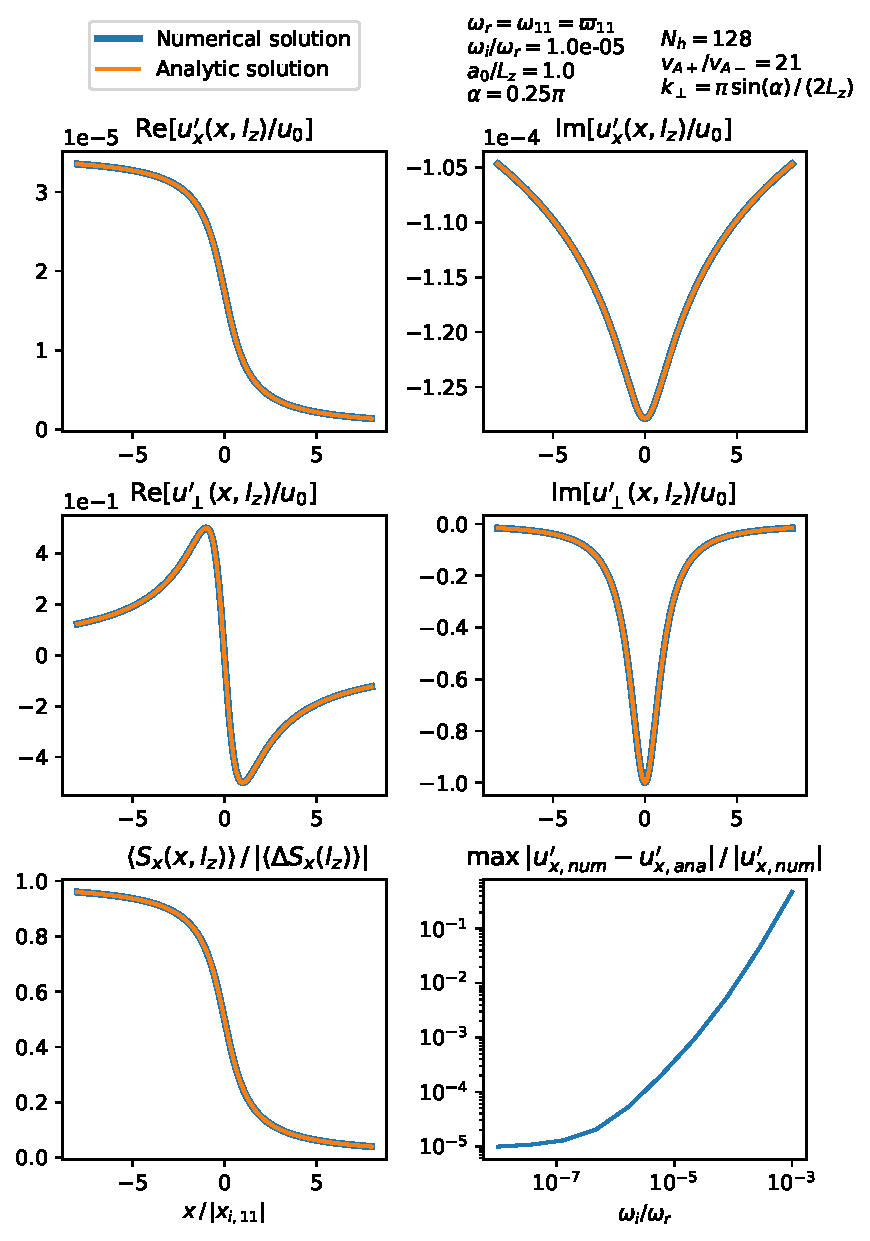
\includegraphics[width=\textwidth,height=0.8\textheight,keepaspectratio]{figures/chapter04/oblique_field_spectral_method_along_x.pdf}
    \vspace{-10pt}
    \caption{This figure shows plots of the real and imaginary parts of $u_x'$ (top row), $u_\perp'$ (middle row) and $\langle S_x' \rangle$ (bottom left) as a function of $x$ at $z=l_z$. We calculated the blue curves numerically and the orange curves plot Equations \eqref{eq:chap_4_oblique_u_perp_final}, \eqref{eq:chap_4_oblique_ux_final} and \eqref{eq:oblique_field_poy_flux_ana}. The bottom right plot shows the relative error between the numerical and analytic solutions for $u_x$ as a function of $\omega_i / \omega_r$. The velocity curves are normalised by $u_0$ which gives the amplitude of $u_\perp$ at $x=0$. The Poynting flux is normalised by $\abs{\langle \Delta S_x' \rangle}$ at $z=l_z$ (see Equation \eqref{eq:chap_4_jump_in_poy_flux}). \textcolor{red}{Need to change log term for $u_x$.}The code used to make this figure is available on GitHub in the following directory:\newline
    \texttt{$\rightarrow$ Python/Chapter4/spectral\_code/line\_along\_x.py}}
    \label{fig:oblique_field_spectral_method_along_x}
    \vspace{-20pt}
\end{figure}

\begin{figure}
    \centering
    \vspace{-20pt}
    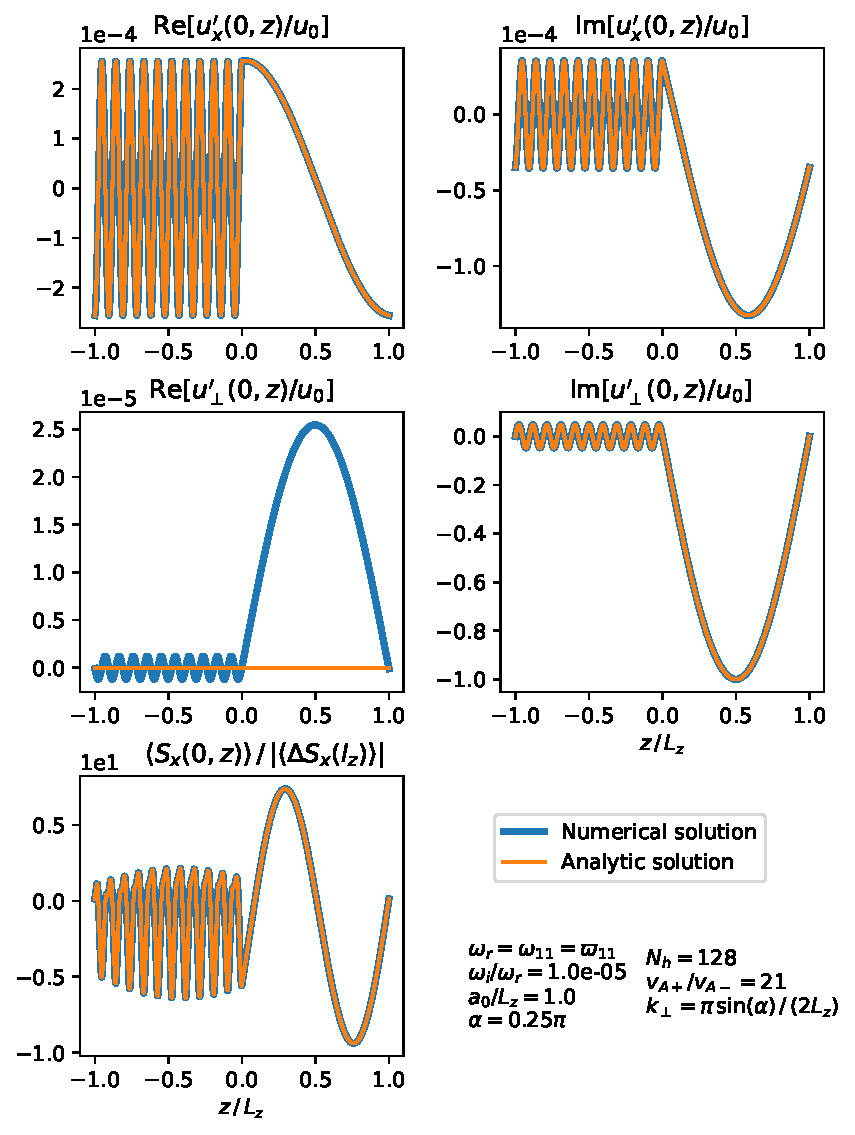
\includegraphics[width=\textwidth,height=0.9\textheight,keepaspectratio]{figures/chapter04/oblique_field_spectral_method_along_z.pdf}
    \vspace{-10pt}
    \caption{This figure is similar to Figure \ref{fig:oblique_field_spectral_method_along_x} except it plots the variables as function of $z$ at $x=0$ instead. The code used to make this figure is available on GitHub in the following directory:\newline
    \texttt{$\rightarrow$ Python/Chapter4/spectral\_code/line\_along\_z.py}}
    \label{fig:oblique_field_spectral_method_along_z}
    \vspace{-20pt}
\end{figure}

To check that the numerical solutions agree with the analytic solutions given by Equations \eqref{eq:chap_4_oblique_u_perp_final}, \eqref{eq:chap_4_oblique_ux_final} and \eqref{eq:oblique_field_poy_flux_ana} and to help visualise the solutions, we plot the solutions in Figure \ref{fig:oblique_field_spectral_method_along_x} and \ref{fig:oblique_field_spectral_method_along_z}. They show that the analytic and numerical solutions do agree provided $\omega_i/\omega_r$ is small enough. The bottom right of the Figure \ref{fig:oblique_field_spectral_method_along_x} shows the maximum relative error between the numerical and analytic solutions for $u_x$, which is given by
\begin{equation}
    \text{max relative $u_x'$ error} = \max_{\substack{-8|x_{i,11}|\le x\le 8|x_{i,11}| \\ -L_z\le z \le L_z}}\abs{\frac{u_{x,num}'-u_{x,ana}'}{u_{x,num}'}},
\end{equation}
where $u_{x,num}'$ denotes the $u_x'$ solution which was calculated numerically and $u_{x,ana}'$ was calculated analytically using Equation \eqref{eq:chap_4_oblique_ux_final}. The bottom right of the Figure \ref{fig:oblique_field_spectral_method_along_x} shows that decreasing $\omega_i/\omega_r$ causes the error to decrease. This plot appears to be converging to a non-zero value and this is because the numerical solution only uses a finite number of harmonics $N_h$. Increasing $N_h$ acts to reduce the error further. Figure \ref{fig:oblique_field_spectral_method_along_z} shows that although the amplitude of $u_\perp$ may decrease significantly in the chromosphere, this is not necessarily true for $u_x$. Equation \eqref{eq:oblique_field_uniform_in_x_ux10-} also shows that $u_x$ in the chromosphere will not necessarily go to zero, even if $v_{A-}\rightarrow0$. This suggests that imposing line-tied ($\vec{u}=0$) boundary conditions at the edge of the corona will lead to the generation of unphysical structures. The usual justification for imposing line-tied boundary conditions is that the chromosphere is significantly denser than the corona and so it acts like a solid wall. Here, $v_{A+}/v_{A-}=21$ and yet $u_x$ is showing no signs of going to zero in the chromosphere. Although $u_x$ does not go to zero, the kinetic energy and magnetic energy is dominated by $u_\perp$ and $b_\perp$, therefore, the kinetic and magnetic energy is approximately uniformly distributed along $z$.

\section{Discussion and conclusions}
\label{sec:chap_4_conclusions}

The primary aim of this chapter is to test if line-tied boundary conditions cause unphysically large boundary layers/evanescent fast waves to form in resonant absorption experiments. To test this, Section \ref{sec:oblique_field_uniform_density_profile_with_line_tied_bcs} calculated the solutions with line-tied boundary conditions imposed and Section \ref{sec:oblique_field_piecewise_constant_density_profile} calculated the solutions with the chromosphere included in the model instead. We compared results from both sections and found that the boundary layers only appear in the leading order solution for $u_x$ in the model with line-tied boundary conditions, they are absent if the chromosphere is included.
This shows that imposing line-tied boundary condition causes the model to overestimate significantly the amplitude of the evanescent fast waves/boundary layers. Note that Sections \ref{sec:oblique_field_uniform_density_profile_with_line_tied_bcs} and \ref{sec:oblique_field_piecewise_constant_density_profile} used a background Alfv\'en speed which did not depend on $x$ so resonant absorption could not occur. However, we simulated the conditions near a singularity in a resonant absorption experiment by imposing very short length scales in $x$. To help verify the conclusions made from Section \ref{sec:oblique_field_uniform_density_profile_with_line_tied_bcs} and \ref{sec:oblique_field_piecewise_constant_density_profile} we used an Alfv\'en speed which depended on $x$ in Section \ref{sec:oblique_field_resonant_absorption}. This enabled resonant absorption to occur and we confirmed that near the singularity the boundary layers are absent in the solution for $u_x$ and $u_\perp$ to leading order. We believe line-tied boundary conditions are useful for their simplicity and convenience, provided their flaws and limitations are understood.

Section \ref{sec:chap_4_energy_equations} showed that oscillations in the $x$ and $\vec{\hat{B}}_0$ directions couple to the oscillations in the $\perp$ due to gradients in the magnetic pressure perturbation, $B_0b_{||}/(2\mu)$. Resonant absorption occurs where the mode conversion is one-way from fast wave perturbations to Alfv\'en waves. 

In Section \ref{sec:normal_field_resonant_absorption_with_line_tied_bcs} our goal was to introduce resonant absorption by using a model which was a simple as possible whilst complex enough to show some of its key properties. For simplicity, we chose the background magnetic field to be at right-angles to the $z=\text{constant}$ plane, i.e. $\alpha=0$ and the background Alfv\'en speed to be a function of just $x$. We calculated the normal mode solutions and derived a single ODE which $u_y$ satisfies, see Equation \eqref{eq:chap_4_uy_ode}. To solve the ODE we used method of Frobenius and showed that the solution can become singular at resonant locations $x_{res,n}$ where $\mathcal{L}_n(x_{res,n})=0$, i.e. at locations where the Alfv\'en wave equation is satisfied. This shows that resonant absorption occurs at locations where the frequency of the driver equals the natural Alfv\'en frequency of a field line. We calculated the leading order approximations of the singular solutions and verified these numerically via a graphical approach in Figure \ref{fig:normal_mode_along_x_alpha=0}.

In Section \ref{sec:oblique_field_uniform_density_profile_with_line_tied_bcs} we used a uniform background Alfv\'en speed and imposed line-tied boundary conditions at $z=0$. We imposed an incident Alfv\'en wave from $z>0$ and calculated the unique solution which ensures $u_x=u_\perp=0$ at $z=0$. After that, we calculated asymptotic expansions for the solution, see Equations \eqref{eq:chap_4_oblique_ux1}-\eqref{eq:chap_4_oblique_b_par3} for $k_x\rightarrow\infty$. We solve for the large $k_x$ limit as this simulates the singularities which form in resonant absorption experiments. Equations \eqref{eq:chap_4_oblique_ux1}-\eqref{eq:chap_4_oblique_ux3} show that $u_x$ contains an evanescent fast wave/boundary layer term to leading order. This is in agreement with similar results found in, for example, \citet{Halberstadt1993,Halberstadt1995,Arregui2003}. Note that the fast wave terms go to zero if $\alpha=0$, i.e. if the background magnetic field is perpendicular to the transition region.

Section \ref{sec:oblique_field_piecewise_constant_density_profile} used a similar model to Section \ref{sec:oblique_field_uniform_density_profile_with_line_tied_bcs} except the Alfv\'en speed was piecewise constant in $z$ instead of uniform. We imposed an incident Alfv\'en wave from $z>0$ and calculated the unique solution which ensures continuity of $u_x$, $u_\perp$, $\pdv*{u_x}{z}$, $\pdv*{u_\perp}{z}$ at $z=0$. After that, we calculated asymptotic expansions for the solution, see Equations \eqref{eq:oblique_field_uniform_in_x_ux10-}-\eqref{eq:oblique_field_uniform_in_x_b_par30+} for $k_x\rightarrow\infty$. They show that fast wave terms are negligible in $u_x$ and $u_\perp$ to leading order. Compare this with Section \ref{sec:oblique_field_uniform_density_profile_with_line_tied_bcs} which showed that the solution for $u_x$ contains a boundary layer term to leading order. Therefore, imposing line-tied boundary conditions can cause the model to overestimate significantly the boundary layers to leading order and we believe we are the first authors to demonstrate this. For the asymptotic series to be valid, we showed that Equation \eqref{eq:chap_4_kx_condition} needs to be satisfied. Hence, for finite $k_x$, if $v_{A-}\rightarrow0$, then the boundary layer terms can be of equal order to the Alfv\'en wave terms in $u_\perp$. However, in a resonant absorption experiment, near the singularity, $k_x\rightarrow \infty$ causing Equation \eqref{eq:chap_4_kx_condition} to be satisfied for any non-zero $v_{A-}$.

Finally, section \ref{sec:normal_field_resonant_absorption_with_line_tied_bcs} aimed to check that $u_x$ and $u_\perp$ contain no boundary layer terms to leading order in resonant absorption experiments. The Alfv\'en speed was piecewise constant in $z$ and dependent on $x$. We imposed periodic boundary conditions for convenience and to ensure the solution is unique. These boundary conditions model a loop which goes through the corona, into the chromosphere, back into the corona and so on. In Section \ref{sec:oblique_field_resonant_absorption_analytic_soln} we calculated the leading order singular solutions near a resonant location analytically. Section \ref{sec:oblique_field_resonant_absorption_numerical_soln} verified the analytic solutions using eigenfunctions to convert the PDEs into a set of ODEs which we solved numerically. Figures \ref{fig:oblique_field_spectral_method_along_x} and \ref{fig:oblique_field_spectral_method_along_z} plot the analytic and numerical solutions side-by-side and show that they agree. We verified that the boundary layers terms are absent in the leading order solution for $u_x$ and $u_\perp$ near the singularity and this confirms that imposing line-tied boundary conditions causes the model to overestimate significantly the amplitude of the boundary layers. However, in Section \ref{sec:oblique_field_uniform_density_profile_with_line_tied_bcs} we showed as $k_x\rightarrow\infty$ the amplitude of the boundary layers does not increase. This suggests that the boundary layers have a limited effect on the rate at which the resonant absorption occurs. Moreover, since the boundary layers are evanescent, they cannot directly transport energy away.

\textcolor{red}{I could add an appendix which calculates the reflection coefficient as a function of $k_x$ and $v_{A-}$ in the piecewise constant domain. This is interesting as it shows how energy may be able to leak into the corona more easily than a naive calculation with just Alfv\'en waves might give.}

\textcolor{red}{I could add an appendix which calculates solution for the case where an incident fast wave is used instead of an incident Alfv\'en wave.}

 
\chapter{Conclusions and future work}
\label{chap:conclusions_and_future_work}
This thesis used mathematical models to develop our understanding of MHD waves in the solar corona.
We chose our models to be complex enough to allow the phenomena we are interested in to be studied and simple enough to be easily understood. We calculated analytic solutions and then verified many of these results numerically by comparing them side-by-side using graphs. The work presented here may play a role in solving the coronal heating problem and developing coronal seismology. 

Chapter \ref{chap:ideal_footpoint_driven_alfven_waves} introduced some of the key concepts relevant to the rest of this thesis. We modelled linear ideal Alfv\'en waves which we injected into the corona by using a footpoint driver. The waves were modelled as perturbations on a uniform background magnetic field and Alfv\'en speed. To begin with, we used a sinusoidal driver in a closed loop and found that the form of the solution was highly dependent on the driver frequency. If the driver frequency equalled one of the natural Alfv\'en frequencies of the loop, then resonance occurred. This meant that the energy grew quadratically with time. If the driver frequency was not equal to a natural frequency, then the energy oscillated about a finite value at the beating frequency (which goes to zero as the driver frequency tends towards natural frequencies). We showed that a white and red noise force driver causes the energy to grow linearly with time on average. A white noise driver is a random driver which excites all frequencies with equal force, and a red noise driver has a power spectrum which goes as $f^{-2}$, where $f$ denotes frequency. In Section \ref{sec:noisy_force} we give a more precise definitions. Observational evidence (see Figure \ref{fig:power_spectrum_morton}) suggests the power spectrum slope for waves in the corona lies somewhere in between $f^{-2}$ and $f^0$. We also considered the case where the waves were partially confined in a leaky loop where a fraction $R<1$ of the incident wave amplitude reflects at the boundary. We used a sinusoidal driver and found leakage prevents the system's energy from growing to infinity, and the system converges towards a steady-state. At steady-state, the waves' amplitude is fixed, and the system oscillates at the driver frequency. Note that a system will also converge towards a steady-state if resistivity or viscosity is included in the model.

Chapter \ref{chap:resistive_phase_mixed_alfven_waves} our goal was to answer whether the dissipation of phase-mixed Alfv\'en waves plays an essential or negligible role in coronal heating? To achieve this goal, we introduced a term called the damping rate per unit of wave energy which we denote $\gamma$. We estimated that for phase mixing to be a viable heating mechanism then our phase mixing model needs to have a $\gamma$ of about $10^{-1}\si{.s^{-1}}$. We are careful to ensure any simplifications we make act to increase $\gamma$, which means our calculation for $\gamma$ is an upper bound. For example, we assume the system is at steady-state which acts to increase $\gamma$, in \citet{Arregui2015} they argue that Alfv\'en waves may not have time to reach steady-state due to thermodynamic changes in the loop. We first introduced phase mixing in an open-loop and calculated the analytic solution using the method of multiple scales. Neighbouring field lines had different natural frequencies, which meant steep gradients formed perpendicular to the velocity and magnetic fields. After that, we modelled a closed-loop and extended our solution for the open-loop using a method of images approach to calculate the analytic solution. We included leakage into the model and found that this acts to reduce $\gamma$. This chapter's results suggest that the dissipation of the gradients produced by phase mixing plays a negligible role in coronal heating. However, it is possible that phase mixing plays a less direct role; for example, it could trigger the Kelvin-Helmholtz and tearing mode instabilities which cause a turbulent cascade. In this case, the dissipation will occur primarily due to gradients parallel to the velocity and magnetic fields because the $\vec{W}^{(0)}$ component of the viscosity tensor will dominate. Note that the gradients formed by phase mixing are perpendicular to the velocity field and magnetic field.

In the resonant absorption literature, authors typically assume the background magnetic field is perpendicular to the transition region. \citet{Halberstadt1993,Halberstadt1995,Arregui2003} use line-tied boundary conditions in their resonant absorption models to show that if the background magnetic field is oblique to the transition region then steep boundary layers / evanescent fast waves can form. The goal in Chapter \ref{chap:resonant_absorption_in_an_oblique_field} was to check that these boundary layers are physical and not a result of approximating the steep jump in density from the corona to the chromosphere with line-tied boundary conditions. To test this, we first introduced resonant absorption in a model where the background field is normal to the transition region and the Alfv\'en speed was purely a function of $x$ to show some of the key properties of resonant absorption. We showed resonant absorption occurs where the frequency of the incoming fast waves equals the natural Alfv\'en frequency of a resonant field line resulting in the formation of singularities at discrete $x$-coordinates. At the singularities, the mode conversion from fast waves to Alfv\'en waves is one-way and is caused by gradients in the magnetic pressure. After that, we modified the model to let the background Alfv\'en speed be uniform in $x$ and piecewise constant in $z$, where $z>0$ models the corona and $z<0$ corresponds to the chromosphere. This meant resonant absorption could not occur. However, we derived dispersion relations and simulated the singularities which would form in a resonant absorption experiment by letting $k_x\rightarrow \infty$. We used an asymptotic expansion to express the solutions in a simpler form for $k_x\rightarrow \infty$. If line-tied boundary conditions are used then $u_x$ to leading order contains a steep evanescent fast wave/boundary layer term to leading order. However, if the chromosphere is included in the model then the steep boundary layers do not appear in the leading order expansion for $u_x$. This suggests that imposing line-tied boundary conditions can cause the model to significantly overestimate the amplitude of the boundary layers. Finally, we extended the model to let the Alfv\'en speed have an $x$-dependence. By using an eigenfunction approach we showed that near singularity / resonant location the boundary layers are not present to leading order. This helps to confirm that line-tied boundary conditions can cause significant overestimation of the size of the boundary layers. However, line-tied boundary conditions can still be useful in future models for their simplicity, provided their limitations are understood. In the future, we would like to compare resonant absorption experiments where line-tied boundary conditions and where the chromosphere is included in the model to precisely quantify the effects of imposing line-tied boundary conditions in a resonant absorption experiment. Also, we would like to extend our results from the Cartesian coordinate system to a cylindrical coordinate system as this can more easily be applied to coronal loops.

This thesis focused on improving our understanding of MHD waves and pushing the boundaries of our current knowledge. We hope that results from the work presented here lead to developments in coronal seismology. In the future, we aim to apply contemporary MHD wave theory to observational data to infer approximate values for difficult to measure quantities, e.g. the magnetic field strength and density. Calculating the values of quantities in the corona could lead to significant developments in explaining the observed dynamics and may present us with new puzzles to solve. With ever-improving computational power and observational instruments, coronal seismology is becoming an increasingly important and relevant area of research. For coronal seismology to become more widely used, we need to develop more user-friendly code and software to automate much of the process. We hope to create software and code that enables users to estimate quantities using coronal seismology quickly. Ideally, the code and software would be easy to use such that the user does not need extensive knowledge of MHD wave theory to estimate the desired quantities. 

Another suggestion for future work is to investigate if the viscous dissipation of fast waves plays a significant role in the quiet sun. In \citet{Withbroe1977,Parker1991} they suggest that the waves need to dissipate over a length scale of 1 or 2 solar radii to heat the corona. In Appendix \ref{adx:coronal_heating_by_viscous_fast_waves}, we use a simple toy model to show that the fast waves can dissipate over short enough length-scales. However, we make many simplifications and so a more extensive analysis is required. 

It has been a privilege to have had this opportunity to contribute towards solar physics research. We hope that the readers found this thesis interesting and useful for developing their understanding of solar/plasma physics. Acquiring a better knowledge of solar/plasma physics at a theoretical level may play a key role in solving problems such as the coronal heating problem which could reveal new and exciting problems which need to be solved. Developments in coronal heating could lead to results in other areas such as nuclear fusion due to our improved understanding of plasma physics.  Finally, it could be relevant for space weather prediction,  which is increasingly important with our ever-increasing dependence on orbital satellites.

\appendix
\chapter{Coronal heating by viscous fast waves}
\label{adx:coronal_heating_by_viscous_fast_waves}
In this appendix, we expand upon a proposed topic for further research mentioned in Chapter \ref{chap:conclusions_and_future_work}. Namely, the possibility that the viscous dissipation of fast waves plays a major role in coronal heating. We will present a simple toy model to show our proposal's plausibility and then discuss how to investigate this rigorously in the future.

\section{Model and assumptions}

In this section, we will describe the model we will use. Our domain is designed to approximate the quiet sun conditions near the equator. We model perturbations on a static background equilibrium and make the same assumptions as those described by Equation \eqref{eq:linear_assumotion_v}-\eqref{eq:linear_assumotion_rho}.The plasma is modelled as cold, i.e. $\beta=0$, which means the magnetic pressure force is negligible. We assume the Lorentz force dominates and neglect the gravitational force. Our background quantities are assumed to be uniform with the background magnetic field pointing south to north and approximately tangential to the solar surface at the equator,
\begin{equation}
    \vec{B}_0 = B_0\vec{\hat{z}},
\end{equation}
The $\vec{\hat{x}}$ direction points radially outwards from the solar surface.

We model the linearised momentum equation as
\begin{equation}
    \pdv{\vec{u}}{t}=v_A^2\qty[\pdv{\vec{\hat{b}}}{z}-\grad \hat{b}_z] + \frac{1}{\rho}\div{\vec{\pi}_0},
\end{equation}
and the linearised induction equations as
\begin{equation}
    \pdv{\vec{\hat{b}}}{t}=\pdv{\vec{u}}{z} - \div{\vec{u}}\,\vec{\hat{z}},
\end{equation}
where $\vec{\pi}_0$ denotes the linearised viscosity tensor (see Equation \ref{eq:braginskii_viscous_stress_tensor}) and
\begin{equation}
    \vec{\hat{b}} = \frac{\vec{b}}{B_0}.
\end{equation}
We assume $\omega_{ci}/\nu_i\ll1$ and neglect the $\vec{W}^{(1)}$, $\vec{W}^{(2)}$, $\vec{W}^{(3)}$, $\vec{W}^{(4)}$ terms. \citet{Mocanu2008} shows that the linearised viscosity tensor is given by
\begin{equation}
\begin{aligned}
    \vec{\pi}_0 &= \eta_0\qty(\vec{\hat{B}}_0 \otimes \vec{\hat{B}}_0 - \frac{1}{3}\vec{I})Q \\
    % &= \eta_0\qty(\vec{\hat{z}} \otimes \vec{\hat{z}} - \frac{1}{3}\vec{I})Q \\
    &=\frac{\eta_0}{3}\begin{pmatrix}
    -1 & 0  & 0 \\
    0  & -1 & 0 \\
    0  & 0  & 2  \\
    \end{pmatrix} Q,
\end{aligned} 
\end{equation}
where $\eta_0$ is given by Equation \eqref{eq:braginskii_eta_0} and 
\begin{gather}
    \vec{\hat{B}}_0 = \frac{\vec{B}_0}{B_0}, \\
    Q = 3\vec{\hat{B}}_0\vdot\grad(\vec{\hat{B}}_0\vdot\vec{u}) - \div{\vec{u}}
\end{gather}
We will assume our variables are of the form
\begin{equation}
    \label{eq:apdx_exp_form}
    f(x,t) = f_0\exp[i(k_x x + \omega t)],
\end{equation}
where $\omega\in \mathds{R}^+$ and $k_x\in \mathds{C}$. This simulates waves, propagating/decaying radially outwards/inwards from the solar surface at the equator. Enforcing $\pdv*{}{y}=\pdv*{}{z}=0$ causes
\[\pdv{}{t}\vec{u}\vdot\vec{\hat{y}}=\pdv{}{t}\vec{u}\vdot\vec{\hat{z}}=\pdv{}{t}\vec{\hat{b}}\vdot\vec{\hat{z}}=\pdv{}{t}\vec{\hat{b}}\vdot\vec{\hat{y}}=0\] 
and we let
\begin{gather}
    \vec{u} = u_x \vec{\hat{x}}, \\
    \vec{\hat{b}} = \hat{b}_z \vec{\hat{z}}.
\end{gather}
Hence,
\begin{gather}
    Q = -\pdv{u_x}{x}, \\
    \label{eq:ux_eqn1}
    \pdv{u_x}{t} = -v_A^2\pdv{\hat{b}_z}{x} + \nu_0\pdv[2]{u_x}{x}, \\
    \label{eq:bz_eqn1}
    \pdv{\hat{b}_z}{t} = -\pdv{u_x}{x}.
\end{gather}

We model the system as weakly viscous and assume that
\begin{equation}
\begin{aligned}
    \epsilon &= \frac{\nu_0 \omega}{v_A^2} \\
    &\approx 1.13\times10^{-1}\qty(\frac{\ln\Lambda}{20})^{-1}\qty(\frac{T}{3\times 10^6\si{.K}})^{5/2}\qty(\frac{\rho}{10^{-13}\si{.kg.m^{-3}}})^{-1} \\
    & \qquad\qquad\qquad\qty(\frac{\omega}{\pi\times10^{-2}\si{.s^{-1}}})\qty(\frac{v_A}{4\times10^5\si{.m.s^{-1}}})^{-2} \\
    &\ll 1.
\end{aligned}
\end{equation}

\section{Damping length}

In \citet{Withbroe1977,Parker1991} they suggest that the waves need to decay on a length scale of 1-2$R_\odot$ to play a significant role in coronal heating, where $R_\odot$ denotes the solar radius. This section aims to to derive a dispersion relation for the waves in our model to calculate a damping length. Taking the time derivative of \eqref{eq:ux_eqn1} to eliminate $\hat{b}_z$ gives
\begin{equation}
    \pdv[2]{u_x}{t} = v_A^2\pdv[2]{u_x}{x} + \nu_0\pdv{}{t}\pdv[2]{u_x}{x}.
\end{equation}
Dividing through by $v_A^2$ and assuming $u_x$ is of the form given by Equation \eqref{eq:apdx_exp_form} gives
\begin{equation}
    \frac{\omega^2}{v_A^2} = (1+i\epsilon)k_x^2.
\end{equation}
Using the binomial expansion gives
\begin{equation}
    k_x^2 = \frac{\omega^2}{v_A^2}\qty[1 -i\epsilon + O(\epsilon^2)].
\end{equation}
We assume $k_x$ is given by the negative root as the waves propagate away from the solar surface in the positive $x$-direction. Hence,
\begin{equation}
    k_x = -\frac{\omega^2}{v_A^2}\qty[1 -\frac{1}{2}i\epsilon + O(\epsilon^2)].
\end{equation}
The decay length-scale is given by
\begin{equation}
    \label{eq:apdx_decay_length}
    \begin{aligned}
    L_d &= \frac{2\pi}{\Im(k_x)} \\
    &\approx4\pi\frac{1}{\epsilon}\frac{v_A^2}{\omega^2} \\
    &= 4\pi\qty(\frac{1}{\nu_0})\frac{v_A^3}{\omega^2} \\
    &= 4\pi\qty(\frac{3}{2.21}\times10^{16}\ln\Lambda\, T^{-5/2}\rho)\frac{v_A^3}{\omega^2}\\
    &\approx 1.42\times10^9\qty(\frac{\ln \Lambda}{20})\qty(\frac{T}{3\times10^6\si{.K}})^{-5/2}\qty(\frac{\rho}{10^{-13}\si{.kg.m^{-3}}})\qty(\frac{v_A}{4\times10^5\si{.m.s^{-1}}})^3 \\
    &\qquad\qquad\qquad\qty(\frac{\omega}{\pi\times10^{-2}\si{.s^{-1}}})^{-2}\si{.m},
    \end{aligned}
\end{equation}
Equation \eqref{eq:apdx_decay_length} suggests that for typical coronal values, it is possible that fast waves could decay on a length-scale about 2 solar radii, $R_\odot\approx 7\times10^8\si{.m}$. Our values for the density and Alfv\'en speed come from mean observed values and were taken from Table 1 in \citet{Morton2016}. Figure \ref{fig:power_spectrum_morton} shows that we chose a high frequency (where $\omega= 2\pi f$) and we discuss this further in the next section.

\section{Discussion}

We have shown that our model can dissipate fast waves on a length-scale of about 2 solar radii, and this suggests that this mechanism could play a significant role in coronal heating. However, we made many simplifications in our analysis, and it is unclear if relaxing these assumptions will increase or decrease the damping length. For example, we modelled the quantities as uniform and linear. This meant waves could not reflect and prevents reflection-driven turbulence \citep{Hollweg1986a,vanBallegooijen2011,Shoda2019}. Authors typically study Alfv\'en wave turbulence, but we think it could be interesting to investigate fast wave turbulence as these are compressible and therefore dissipate via viscosity more easily. We used a high frequency in \eqref{eq:apdx_decay_length} to account for the fact that waves may be able to cascade to higher frequencies due to turbulence. Including a more complex field can lead to several effects such as fast wave refraction towards null points \citep{McLaughlin2006,McLaughlin2011,McLaughlin2016}, the triggering of reconnection \citep{McLaughlin2009} and enhanced phase mixing \citep{Similon1989,Howson2020a}. We modelled the fast waves as propagating perpendicular to the field, in reality a component will propagate parallel and this could decrease the heating. Therefore, we would expect less heating at coronal holes where the field is approximately normal to the solar surface. In summary, the results provided here suggest further study could be fruitful. However, a more extensive analysis is needed to determine if fast waves' viscous dissipation plays a significant role in coronal heating.

\bibliographystyle{chicago}
\bibliography{references}

\end{document}